\documentclass[12pt, twoside,a4paper,toc=bibliography]{scrbook}
\usepackage{doc}
\usepackage{a4wide}
\usepackage{makeidx}
\usepackage[tight,footnotesize]{subfigure}
\usepackage{amsmath}
\usepackage{amsfonts}
\usepackage{multirow}
\usepackage{booktabs}
\newtheorem{theorem}{Theorem}
\newtheorem{problem}{Problem}
\newtheorem{definition}{Definition}
\usepackage{graphicx}
\graphicspath{{./figs/}}
%\usepackage{algorithmic}
\usepackage{listings}
\usepackage[utf8]{inputenc}
\usepackage[noend]{algpseudocode}
\usepackage{hyperref}
\hypersetup{
colorlinks,
citecolor=black,
filecolor=black,
linkcolor=black,
urlcolor=black
}

% tikz
%\usepackage{tikz}
%\usetikzlibrary{patterns,shapes,calc,matrix,plotmarks}
%\RequirePackage{ifthen}
% pgf
%\usepackage{pgfplots}

\hyphenation{
	MATLAB
}

\DeclareMathOperator*{\argmin}{arg\,min}
\DeclareMathOperator*{\argmax}{arg\,max}

\usepackage[table]{xcolor}
\newcommand{\figref}[1]{Figure~\protect\ref{#1}}
\newcommand{\secref}[1]{Section~\protect\ref{#1}}
\newcommand{\chapref}[1]{Chapter~\protect\ref{#1}}
\newcommand{\defref}[1]{Definition~\protect\ref{#1}}
\newcommand{\coderef}[1]{Algorithm~\protect\ref{#1}}
\newcommand{\appref}[1]{Appendix~\protect\ref{#1}}



\usepackage{color}
\definecolor{lightgray}{rgb}{.9,.9,.9}
\definecolor{darkgray}{rgb}{.4,.4,.4}
\definecolor{purple}{rgb}{0.65, 0.12, 0.82}
\renewcommand{\ttdefault}{pcr}
\lstdefinelanguage{JavaScript}{
keywords={typeof, new, true, false, catch, function, return, null, catch, switch, var, if, while, do, else, case, break,for,with},
basicstyle=\ttfamily,
keywordstyle=\bfseries,
ndkeywords={class, export, boolean, throw, implements, import},
ndkeywordstyle=\color{darkgray}\bfseries,
identifierstyle=\color{black},
sensitive=false,
comment=[l]{//},
morecomment=[s]{/*}{*/},
commentstyle=\color{purple}\ttfamily,
stringstyle=\color{red}\ttfamily,
morestring=[b]',
morestring=[b]"
}

\lstset{
language=JavaScript,
backgroundcolor=\color{lightgray},
extendedchars=true,
basicstyle=\footnotesize\ttfamily,
showstringspaces=false,
showspaces=false,
numbers=left,
numberstyle=\footnotesize,
numbersep=9pt,
tabsize=2,
breaklines=true,
showtabs=false,
captionpos=b
keywords={with},
}
\renewcommand{\lstlistingname}{Algorithm}

\newcommand{\nreq}{L}
\newcommand{\req}{M}
\newcommand{\setR}{\ensuremath{\mathbb{R}}}
\newcommand{\col}{\ensuremath{c}}
\newcommand{\row}{\ensuremath{r}}
\newcommand{\field}[1]{\mathbb{#1}}
\newcommand{\R}{\ensuremath{\field{R}}}
\newcommand{\todo}[1]{\textbf{#1}}
\newcommand{\nnz}[1]{\ensuremath{\operatorname{nz}(#1)}}
% Define the name of the two minimization problems
\newcommand{\MinStaBic}{\textsc{Minimum Star Bicoloring}}
\newcommand{\MinUniCom}{\textsc{Minimum Unidirectional Compression}}
\newcommand{\MinBidCom}{\textsc{Minimum Bidirectional Compression}}

\newcommand{\MinRStaBic}{\textsc{Minimum Restricted Star Bicoloring}}
\newcommand{\MinRUniCom}{\textsc{Minimum Partial Unidirectional Compression}}
\newcommand{\MinRBidCom}{\textsc{Minimum Partial Bidirectional Compression}}

\begin{document}
\pagenumbering{roman}
\begin{titlepage}
\centering

\includegraphics[width=0.3\linewidth]{logo}
\par
\vspace{1cm}
{\Large\textbf{Combining partial Jacobian computation and preconditioning:
New heuristics, educational modules, and applications}\par}
\vspace{1cm}
{\Large Mohammad Ali Rostami\par}
\vspace{2cm}
{\large Reviewers:\par}
\vspace{0.6cm}
{\Large Prof. Martin B{\"u}cker\par}
{\Large Faculty of Mathematics and Computer Science\\Friedrich Schiller University Jena, Germany\par}
\vspace{1cm}
{\Large Prof. Trond Steihaug\par}
{\Large Faculty of Computer Science\\University of Bergen, Norway\par}
\vspace{1cm}
{\Large \today}
\end{titlepage}
\chapter*{Abstract}
Solving problems originating from real-world applications is often based on the solution of a
system of linear equations whose coefficient matrix is a large sparse Jacobian matrix. Hence, there is
research to exploit the sparsity structure and to decrease the amount of storage. In contrast to full
Jacobian computation in which all nonzero elements are to be determined, partial Jacobian
computation is looking at a subset of these elements. Partial Jacobian computation can therefore
be faster and more efficient than full Jacobian computation. Since Jacobian matrix-vector products
are needed in iterative solvers, these types of linear systems can be efficiently solved using
automatic differentiation. Determining these nonzero elements in full or partial Jacobian
computations by automatic differentiation techniques can be modeled as graph coloring in the
language of graph theory.
%
On the other hand, preconditioning techniques are used to improve the convergence of iterative
solvers and typically need access to all nonzero elements of the Jacobian matrix. So, a sparsification
is applied to the Jacobian matrix before computing the preconditioner. The nonzero elements
obtained from the sparsification are considered as the required elements in a restricted coloring.
Lülfesmann (PhD thesis, RWTH Aachen University, 2012) introduced a procedure that selects a
subset of the remaining nonrequired elements. The approach then adds this subset to the
sparsified matrix such that neither fill-in is created nor an increase in the number of colors happens.
This thesis consists of two parts. In the first part, we look at different ways to optimize the process of
selecting these nonrequired elements. We introduce three new coloring heuristics and compare
them with each other as well as with existing approaches. Also, we look at a particular case in which
we consider only the diagonal elements as required elements. For this case, we generalize a
previous result  and introduce a new coloring heuristic. To evaluate our proposed heuristics in
practice, we apply them to a problem from geoscience. Finally, we describe our new software
package implementing these new heuristics. In the second part of this thesis, we introduce  a
collection of interactive educational modules to teach not only graph coloring, but also other
concepts from combinatorial scientific computing in the classroom. These modules are designed to
involve the students more thoroughly in the process of learning. At the end, we explain the design
of this collection and outline its implementation.

\chapter*{Zusammenfassung}
Die Lösung von realistischen Anwendungsproblemen basiert oft auf der Lösung von linearen
Glei\-chungs\-systemen, deren Koeffizientenmatrizen  große dünnbesetze Jacobi-Matrizen sind.
Deshalb gibt es eine Fülle von Forschungsarbeiten mit dem Ziel, die Struktur dieser Matrizen zur
Reduktion von Rechenzeit und Speicher auszunutzen. Im Gegensatz zu der voll\-ständigen
Berechnung von Jacobi-Matrizen, in der alle Nicht\-null\-elemente be\-stimmt werden müssen,
wird in einer partiellen Berechnung lediglich eine Teilmenge aller Nichtnullelemente be\-stimmt.
Die partielle Be\-rechnung kann daher im Vergleich zu einer vollständigen Berechnung zu
schnelleren und effizienteren Verfahren führen. Da Jacobi-Matrix-Vektor-Produkte in iterativen
Lösern benötigt werden, lassen sich diese Typen von linearen Systemen mit Techniken des
automatischen Differenzierens effizient lösen. Die Be\-stimmung von Nicht\-null\-elemente durch
vollständige oder partielle Berechnungen von Jacobi-Matrizen kann in der Sprache der
Graphen\-theorie als Problem einer Graphen\-färbung modelliert werden.
%
Auf der anderen Seite werden Vor\-konditions\-techniken verwendet, um die Konvergenz von
iterativen Lösern zu verbessern. Solche Vor\-konditions\-techniken greifen meist auf alle
Nichtnullelemente der Jacobi-Matrix zu. Daher kann es vorteilhaft sein, eine Ausdünnung auf die
Jacobi-Matrix anzuwenden, bevor die Vor\-kon\-ditio\-nie\-rung berechnet wird. Die nach der
Ausdünnung verbleibenden Nicht\-null\-elemente werden als benötigte Elemente bezeichnet und
in einer eingeschränkten Färbung verwendet. Lülfesmann (Dissertation, RWTH Aachen, 2012) hat
ein Verfahren eingeführt, das eine Teilmenge der nichtbenötigten Elemente auswählt und zu der
ausgedünnten Jacobi-Matrix hinzufügt, so dass weder Füllelemente noch eine Erhöhung der Anzahl
der Farben erfolgt. Die nun vorliegende Dissertation besteht aus zwei Teilen. Im ersten Teil
be\-trachten wir verschiedene Möglichkeiten, den Prozess der Auswahl dieser nichtbenötigten
Elemente zu optimieren. Wir stellen drei neue Färbungsheuristiken vor und vergleichen sie sowohl
untereinander als auch mit bisherigen Ansätzen. Wir be\-trachten auch einen Spezialfall, in dem als
benötigte Elemente  nur die Diagonalelemente zu be\-stimmen sind. Wir verallgemeinern dabei ein
vorheriges Ergebnis und führen eine neue Färbungsheuristik ein. Um unsere vorgeschlagenen
Heuristiken in der Praxis zu evaluieren, wenden wir sie auf eine Problemstellung aus den
Geo\-wissen\-schaften an. Schließlich be\-trachten wir unser neues Softwarepaket, das die neuen
Heuristiken implementiert. Im zweiten Teil dieser Arbeit stellen wir eine Sammlung von interaktiven
Lehrmodulen vor, die nicht nur Graphenfärbung sondern auch andere Konzepte aus dem
kombinatorischen wissen\-schaftlichen Rechnen im Klassenzimmer illustrieren. Diese Module
wurden ent\-wickelt, um die Studierenden noch gründlicher in den Prozess des Lernens zu
involvieren. Schließlich erläutern wir den Ent\-wurf dieser Sammlung von Lehrmodulen und
beschreiben deren Implementierung.


\chapter*{Acknowledgments}
\noindent This project would not have been possible without the support of many people. I must
express my first gratitude towards my supervisor \textit{Prof.\ Dr.\ Martin B\"ucker} for his
continuous support during my research, patience, immense knowledge, and attention to details. I
should confess that I can not imagine a better and friendlier supervisor. \textit{Prof.\ Dr.\ Trond
Steihaug} was a good listener to my ideas that we discussed at the Oxford conference on
algortihmic differentiation. I like to thank him for accepting to review my thesis. Besides, I would like
to thank \textit{Michael Lülfesmann} for his comments on my work. Finally, I wish to thank my wife
\textit{Masoumeh Seydi} and my best friend \textit{Azin Azadi} for encouraging me throughout all
my studies at university.

\tableofcontents
\chapter{Introduction}
\pagenumbering{arabic}
In scientific computing, it is common to solve a given problem by using methods from combinatorial mathematics.
In particular, graphs are ubiquitous in numerical linear algebra if the underlying matrices are sparse.
This thesis consists of two parts.
In the first part, we discuss new coloring heuristics for the partial Jacobian computation.
In the second part, we introduce a set of interactive educational modules teaching these graph problems in classroom.

This thesis is concerned with
the solution of linear equations whose coefficient matrices are sparse, large, and nonsingular.
Furthermore, it is assumed throughout this thesis that the coefficient matrix is a
Jacobian matrix of some mathematical function.
This Jacobian matrix is computed by Automatic Differentiation (AD)~\cite{Griewank2008EDP,Rall1981ADT} without truncation error.
AD computes a product of a Jacobian and another matrix which is called the seed matrix.
A careful choice of the seed matrix will reduce the computational effort as well as
the storage. Different choices can be formulated as different graph problems.

These systems of linear equations are solved using iterative methods which are in practice
accelerated by preconditioning techniques. Most preconditioning techniques need access to all
nonzero elements of the Jacobian matrix which can lead to performance problems when standard
techniques of AD are employed. Therefore, we consider an alternative approach that first applies a
sparsification operator to the Jacobian matrix and then uses standard preconditioning techniques
for the sparsified matrix. This process becomes complete by adding more nonzero elements to the
sparsified matrix without producing more fill-in elements and without increasing efforts to set up
the resulting sparsified matrix. We introduce new heuristics targeting the careful choice of these
extra nonzero elements.

Our work is based on the idea of exploiting the sparsity pattern of a matrix in favor of reducing the
computational efforts. The assumption here is that the sparsity pattern is known a~priori, for
example, from the formulation of a physical problem. Curtis, Powell, and Reid~\cite{Curtis1974117}
were first to study the determination of a sparse Jacobian matrix based on the sparsity exploitation.
Coleman and Mor{\'e}~\cite{Coleman1983EoS} transformed this sparse matrix problem into the
problem of vertex coloring in graph theory. The idea is to formulate the compression of the
columns (similarly for rows) such that all the nonzero elements of the Jacobian matrix are
determined. This is called unidirectional compression. Later, a bidirectional compression is
introduced and analyzed in~\cite{Coleman1996SaE} and~\cite{hs:csj} which can result in larger
savings in computation and storage. Several other graph models are studied further in Hossain and
Steihaug~\cite{hs:gmei} like the pattern graph which keeps the structure of the matrix explicitly.
Also, a recent graph formulation is to group together rows into blocks and partition the resulting
column segments in~\cite{optimal_diret_determination}. On the other hand, rather than computing
all nonzero elements, some other problems from scientific computing target the computation of
only a proper subset of the nonzero elements. These problems are studied under the term of
partial Jacobian computation. Gebremedhin, Manne, and Pothen~\cite{Gebremedhin05whatcolor}
introduced the rules of the partial Jacobian computation and its corresponding graph problems.
Several examples in the partial Jacobian computation are studied later in \cite{CalotoiuMaster} and
\cite{LulfesmannMaster}.

Lülfesmann~\cite{Lulfesmann2012Fap} introduced for the first time the idea of combining partial
Jacobian computation and ILU preconditioning. This idea defines a sparsification operator $\rho$
which is applied to the Jacobian matrix before the ILU preconditioner is computed. The nonzero
elements selected by $\rho$ are called required elements. The remaining elements are called
nonrequired elements. Lülfesmann~\cite{Lulfesmann2012Fap} computes the seed matrix for
automatic differentiation by considering a graph coloring restricted to these required elements.
Then, a subset of nonrequired elements is added to the set of required elements such that the
number of colors does not increase and no extra fill-in elements are generated in the ILU
preconditioning. These elements are called the additionally required elements. In this thesis, we
extend this idea further as follows. First, we define new coloring heuristics (both for distance-$2$
coloring and star bicoloring) to increase the number of additionally required elements without
having a high increase in the number of colors. Then, we apply these new heuristics to an example
from geoscience. Later, we generalize a previous result from Lülfesmann~\cite{Lulfesmann2012Fap}
for the coloring restricted to diagonal elements. Finally, we introduce a software package to
implement these new heuristics.

In the second part of this thesis, we summarize our previous publications
\cite{2013:05,2014:01,2014:02,2014:09,2015:3,cscpaper} as well as discuss some new features to teach
the coloring heuristics in classroom. In this part, we develop a collection of educational modules for
teaching purposes. Each module illustrates side by side the matrix and graph view of a problem in
scientific computing and its equivalent combinatorial problem, respectively. The student can
interactively follow the steps of the algorithms in this module. We first outline the overall design of
this collection. Then, we discuss the graph coloring module as well as the other available modules.
We explain the new unpublished feature in which an animation of the algorithm is visualized.
Finally, we explain the implementation details of this collection.

This dissertation is structured as follows. First, we discuss the known graph models from scientific
computing in~\chapref{prel}. Then, \chapref{package} discusses our new coloring heuristics.
\chapref{explain} introduces our interactive educational modules. Finally, the conclusion and future
work are presented in \chapref{conc}.

\chapter{Known graph models from scientific computing}
\label{prel}
In this chapter, we briefly discuss known graph formulations and
models needed in this thesis. In each section of this chapter,
we provide some references which explain further these concepts in details.
We look at the ideas to determine the nonzeros of sparse Jacobian matrices in
\secref{s.det.nonzero}.
We look at definitions of combining ILU preconditioning and
partial Jacobian computation in \secref{s.precond}.

%===================================================================================================
\section{Determining nonzeros of sparse Jacobian matrices}
\label{s.det.nonzero}
%===================================================================================================
There are many references on exploiting the sparsity pattern of Jacobian matrices
to improve the performance of automatic differentiation.
Here, we look at full and partial Jacobian computation in~\secref{s.full.jac} and \secref{s.part.jac}.
%===================================================================================================
\subsection{Full Jacobian computation}
\label{s.full.jac}
%===================================================================================================
Assume a program computes a function $f(x) : \setR^n \rightarrow \setR^m$
at the computational cost $t$.
Techniques of automatic differentiation (AD)~\cite{Griewank2008EDP,Rall1981ADT} generate
computer programs capable of evaluating the $m \times n$ Jacobian matrix $J$.
The forward mode of automatic differentiation generates a program automatically
which computes the product of the Jacobian matrix with a given seed matrix $V$,
i.e., $JV$. There is a reverse mode of automatic differentiation which computes the product $WJ$
where $W$ is another seed matrix.
These techniques of automatic differentiation compute the matrix-matrix products $JV$ and $WJ$
without assembling the Jacobian $J$.

Suppose the matrix $V$ has $\col$ columns and the matrix $W$ has $\row$ rows.
The computational costs of these products using the forward and reverse modes
is then given by $\col t$ and $\row t$, respectively.
In general, the Jacobian $J$ is computed choosing either $c=n$ and $V$ as the identity of
order~$n$ in the forward mode or $r = m$ and $W$ as the identity of order $m$ in the
reverse mode. However, if $J$ is sparse and its sparsity pattern is known, the number of
columns of~$V$ in the forward mode or the number of rows of~$W$ in the reverse mode can
be reduced to $\col < n$ or $\row < m$ such that all nonzero entries of $J$ still appear
in the product $JV$ or $WJ$. This way, the computational cost is decreased using either
the forward mode with an appropriate linear combination of the columns of~$J$ or the reverse
mode with a suitable linear combination of the rows of~$J$; see the
survey~\cite{Gebremedhin05whatcolor}.
Later in this chapter, we formulate problems to compute the
minimum values for $\col$ and $\row$ and the corresponding combinatorial problem.
%===================================================================================================
\subsubsection{Scientific computing problem}
\label{ss.problem.full}
%===================================================================================================
Here, we find a seed matrix in which
the corresponding number of rows and columns is smaller than the actual Jacobian matrix which is called compression.
A unidirectional compression is a compression in either rows or columns in contrast to
a bidirectional compression in which both rows and columns are compressed at the same time.
The key idea behind this \emph{unidirectional compression} is now illustrated for the
forward mode. First, we present a definition as follows.
\begin{definition}[Structural Orthogonality]
\label{d:struct_orth}
Let $J=[c_1, c_2, \dots, c_n]$ denote the $m\times n$ Jacobian matrix
in which $c_i \in \setR^m$ is the $i$th
column. Two columns $c_i$ and $c_j$ are
called \emph{structurally orthogonal} if they do not have any nonzero element in a same
row. Two columns are called \emph{structurally non-orthogonal} if there is at least one
row in which both columns, $c_i$ and $c_j$, have a nonzero element.
Analogously, two rows are
\emph{structurally orthogonal} if they do not have any nonzero element in a same column.
\end{definition}
We can compute a linear combination of a group of structurally orthogonal columns of the Jacobian matrix
such that this linear combination contains all elements of these columns.
The definition of the structurally orthogonal columns can be similarly adapted to rows.
It follows that the number of structurally orthogonal groups
represents the computational cost either for columns or rows.
\figref{f.mat-ex-for-orth} (Left) and \figref{f.mat-ex-for-orth} (Middle) show two examples
of matrices which can be compressed efficiently by columns and by rows, respectively.
\begin{figure}
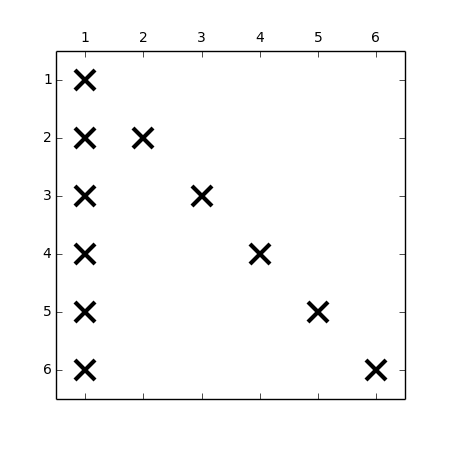
\includegraphics[width=0.3\linewidth]{diag-col}
\hfill
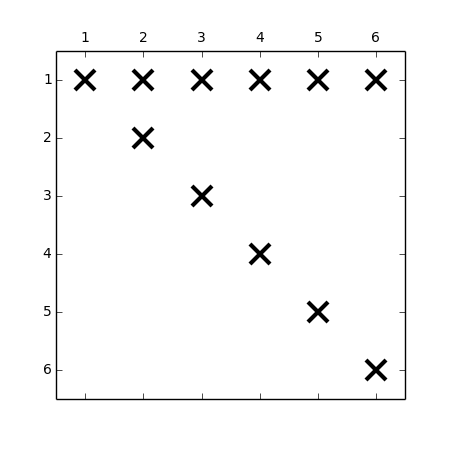
\includegraphics[width=0.3\linewidth]{diagrow}
\hfill
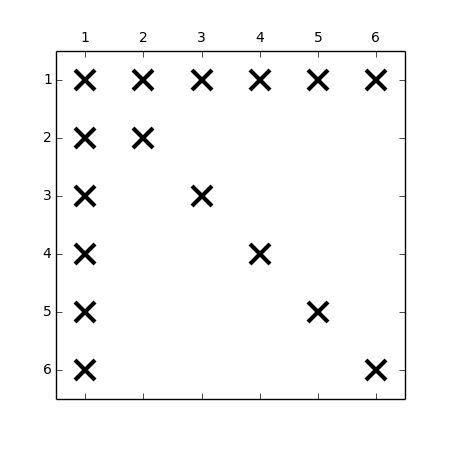
\includegraphics[width=0.3\linewidth]{arrow}
\caption{
(Left) An example of a matrix compressed efficiently by columns.
(Middle) An example of a matrix compressed efficiently by rows.
(Right) An example of a matrix which cannot be compressed efficiently neither by columns nor by rows.
}
\label{f.mat-ex-for-orth}
\end{figure}
Now, consider the matrix in \figref{f.mat-ex-for-orth} (Right) that has neither structurally orthogonal columns nor structurally orthogonal rows.
Therefore, there is no unidirectional compression of the
matrix, neither by columns nor rows.
However, the technique of bidirectional compression,
which compresses both columns and rows at the same time,
will reduce the computational cost for that example.
This technique uses both forward and reverse modes of automatic differentiation.

For general sparsity patterns,
it is not straightforward to figure out how to linearly combine columns and rows such that
the computational cost is minimized. Hence, we introduce the combinatorial
optimization problems~\ref{p.seed.uni} and ~\ref{p.seed.bid}
for unidirectional and bidirectional compression to determine
the nonzero elements of large Jacobian matrices efficiently.

\begin{problem}[\MinUniCom]
\label{p.seed.uni} Let $J$ be a sparse ${m\times n}$ Jacobian matrix with a known sparsity
pattern. Find a binary seed matrix $V$ of dimension $n\times \col$
whose number of columns is minimized
such that all nonzero elements of $J$ also appear in
the matrix-matrix product $JV$.
\end{problem}
The corresponding compression problem for minimizing the number of rows in the matrix-matrix
product $W.J$ is straightforward and omitted here.

\begin{problem}[\MinBidCom]
\label{p.seed.bid} Let $J$ be a sparse ${m\times n}$ Jacobian matrix with known sparsity
pattern. Find a pair of binary seed matrices $V$ of dimension $n\times \col$ and $W$~of
dimension $\row \times m$ in which the number of columns of $V$ and the number of rows of $W$ sum up to a minimal value, $\col + \row$, such that all nonzero elements of $J$ also appear in
the pair of matrix-matrix products $JV$ and $WJ$.
\end{problem}

%==========================================================================================
\subsubsection{Combinatorial model}
\label{s.modeling.full}
%==========================================================================================
We reformulate the scientific computing problems which
we have discussed in \secref{ss.problem.full}.
The new formulation is an equivalent problem defined on a
carefully chosen graph model. The survey \cite{Gebremedhin05whatcolor}
discusses different methods
to exploit the sparsity involved in derivative computations.
We first look at a simple graph model for the unidirectional compression.
%
\begin{definition}[Column Intersection Graph]
\label{d:cig}
The column intersection graph $G = (V,E)$ associated with an $n \times n$ Jacobian matrix $J$
consists of a set of vertices $V=\{v_1, v_2, \dots, v_n\}$ whose vertex $v_i$ represents
the $i$th column $J(:,i)$. Furthermore, there is an edge $(v_i,v_j)$ in the set of edges
$E$ if and only if the columns $J(:,i)$ and $J(:,j)$ represented by $v_i$ and $v_j$
are structurally non-orthogonal.
\end{definition}

As we have a graph model associated with our Jacobian matrix in \defref{d:cig},
the grouping of columns can be encoded in the following well-known graph coloring problem.
%
\begin{definition}[Coloring]
A coloring of $G=(V,E)$ is a mapping $\Phi : V \to \{1, \dots, p\}$ with the property
$\Phi(v_i)\neq \Phi(v_j)$ if $(v_i,v_j) \in E$.
\end{definition}
%
Coleman and Mor\'{e} \cite{Coleman1983EoS} then showed that Problem~\ref{p.seed.uni}, which
asks for a seed matrix with a minimal number of columns, is equivalent to the following
coloring problem.

\begin{problem}[Minimum Coloring]
\label{p:mincol}
Find a coloring $\Phi$ of the column intersection graph $G$
associated with a sparse Jacobian $J$
with a minimal number of colors.
\end{problem}

Although, this model is convincing for the unidirectional compression,
the bidirectional compression can not be an instance of this model.
A bidirectional compression needs the information of both rows and columns. Therefore, a bipartite graph model is defined for this purpose as in~\cite{Coleman1996SaE,cv:ecs,hs:csj}.

\begin{definition}[Bipartite Graph Model]
\label{d.bip.graph}
In the bipartite graph model, the vertex set $V=V_c\cup V_r$
is decomposed into a set of vertices~$V_c$ representing columns of $J$ and another set of
vertices~$V_r$ representing rows. The set of edges~$E$ is used to represent the nonzero
elements and it is defined as follows. An edge $(c_i , r_j) \in E$ connects a column
vertex $c_i \in V_c$ and a row vertex $r_j \in V_r$ if there is a nonzero element in $J$
at the position represented by $c_i$ and $r_j$. The graph is bipartite indicating that
all edges connect vertices from one set~$V_c$ to the other set $V_r$. That is, there is
no edge connecting vertices within the set $V_c$ or within $V_r$. Moreover, two vertices
that are connected by a path of length two, are called \emph{distance-$2$ neighbors}.
\end{definition}

The coloring problem in the column-intersection graph can also be represented in
this bipartite graph model. This equivalent coloring is done only in the set of
column vertices. Also, \emph{distance-$2$ neighbors} should be considered instead of
edges.

The overall idea behind transforming Problem \ref{p.seed.bid}, \MinBidCom, into an equivalent
problem using the bipartite graph model is as follows. The grouping of the columns and
rows is expressed by representing each group by a color. Vertices that belong to the same
group of columns/rows are assigned the same color. Formally, this is represented by a
coloring of a bipartite graph. Such a coloring is a mapping
$$
\Phi:V_c \cup V_r \to \{0,1,\dots ,p\}
$$
that assigns to each vertex a color represented by an integer.
The coloring~$\Phi$ also involves a ``neutral'' color
representing the following ``don't color'' situation. A vertex $v \in V_c \cup V_r$ that is not
used in the grouping of columns/rows is assigned the neutral color $\Phi(v)=0$. More
precisely, if $\Phi(v)=0$ for a column vertex $v$ then every nonzero represented by an
incident edge of $v$ is determined by a linear combination of rows. Similarly, a nonzero
entry represented by an edge that is incident to a neutrally-colored row vertex is
determined by a linear combination of columns.

To represent the process of finding seed matrices using the bipartite graph model, it is
necessary to consider the underlying properties, which are as follows:
\begin{enumerate}
\item The computational cost roughly consists of the number of groups of structurally orthogonal columns and
rows. Since the overall cost is the sum of the costs associated with the forward mode
and the reverse mode, the (non-neutral) colors for the forward mode and the
(non-neutral) colors for the reverse mode need to be different.

\item It may happen that some nonzero
elements may be computed twice, by the forward mode in $JV$ and by the reverse mode
in $WJ$. Therefore, an edge representing such a nonzero element connects two
vertices with two different non-neutral colors. In general, since the
\MinBidCom~problem asks for computing \emph{all} nonzero elements, at least one vertex of
every edge has to be colored with a non-neutral color.

\item Suppose two columns are structurally non-orthogonal and have a nonzero element in a
same row. If this row is not handled by the reverse mode, these two columns need to
be in different column groups. The same argument holds for corresponding situations
with row groups.

\item Consider three nonzero elements in the matrix positions $(i,k)$, $(i,\ell)$, and
$(j,k)$. Suppose that the nonzero at $(i,k)$ is computed by the reverse mode
assigning some (non-neutral) color to the row vertex $r_i$. Then, if $(j,k)$ is
also computed via the reverse mode, a second (non-neutral) color is needed for
$r_j$. Now, if $(i,\ell)$ is already determined by the reverse mode for the row $i$ the
column vertex $c_\ell$ is assigned the neutral color. However, if $(i,\ell)$ is
computed by the forward mode, a third (non-neutral) color is needed for $c_\ell$. A
similar argument holds if $(i,k)$ is computed by the forward mode.
\end{enumerate}

Based on these considerations, the following definition captures these properties.

\begin{definition}[Star Bicoloring]\label{d.coloring}
Given a bipartite graph $G=(V_c\cup V_r, E)$, then a mapping $\Phi:V_c \cup V_r \to
\{0,1,\dots ,p\}$ is a star bicoloring of $G$ if the following conditions are satisfied:
\begin{enumerate}
\item Vertices in $V_c$ and $V_r$ receive disjoint colors, except for the neutral color~$0$. That
is, for every $c_i \in V_c$ and $r_j \in V_r$, either $\Phi(c_i) \neq \Phi(r_j)$ or
$\Phi(c_i)=\Phi(r_j)=0$.

\item At least one vertex of every edge receives a non-neutral color. That is, for every
$(c_i,r_j)\in E$, the conditions $\Phi(c_i)\neq 0$ or $\Phi(r_j)\neq 0$ hold.

\item For every path $(u,v,w)$ with $\Phi(v) = 0$, the condition $\Phi(u)\neq \Phi(w)$ is
satisfied.
\item Every path of length three with four vertices uses at least three colors
(possibly including the neutral color).
\end{enumerate}
\end{definition}

Using the bipartite graph model and the definition of a star bicoloring, the problem
\MinBidCom\ is equivalent to the following graph problem.

\begin{problem}[\MinStaBic]
\label{p.coloring} Given the bipartite graph $G=(V_r\cup V_c, E)$ associated with a sparse Jacobian
matrix~$J$, find a star bicoloring of $G$ with a minimal number of non-neutral colors.
\end{problem}

A unidirectional compression is a special case of a bidirectional compression. More precisely, a
unidirectional compression with respect to columns corresponds to a star bicoloring in which all
the vertices in $V_c$ are colored with a non-neutral color and all row vertices are colored with
the neutral color. This way, the coloring constraint of a star bicoloring reduces to the coloring of
distance-$2$ neighbors in the bipartite graph using different (non-neutral) colors. This distance-2
coloring in the bipartite graph model is then equivalent to a coloring in the undirected graph
model in which all neighbors are colored differently. Finally, a discussion of the computational
complexity of Problem~\ref{p.coloring} including recent new results is given in~\cite{jj:cjr}.

%To illustrate the tricky transformation from \MinBidCom\ to \MinStaBic, we design a new
%educational module explained in Section~\ref{s.bidirectional}.
%%%%%%%%%%%%%%%%%%%%%%%%%%%%%%%%%%%%%%%%%%%%%%%%%%%%%%%%%%%%%%%%%%%%%%%%%%%%%%%%%%%%%%%%%%%%%%%%%%%%%%%%%
\subsection{Partial Jacobian computation}
\label{s.part.jac}
%%%%%%%%%%%%%%%%%%%%%%%%%%%%%%%%%%%%%%%%%%%%%%%%%%%%%%%%%%%%%%%%%%%%%%%%%%%%%%%%%%%%%%%%%%%%%%%%%%%%%%%%%
Gebremedhin et al.~\cite{Gebremedhin05whatcolor} introduced the concept of partial Jacobian computation
in which only a subset of the nonzero Jacobian entities, the required elements, are to be determined.
L{\"u}lfesmann~\cite{Lulfesmann2012Fap} studied this area in more details and
introduced some heuristics for partial computation.
%%%%%%%%%%%%%%%%%%%%%%%%%%%%%%%%%%%%%%%%%%%%%%%%%%%%%%%%%%%%%%%%%%%%%%%%%%%%%%%%%%%%%%%%%%%%%%%%%%%%%%%%%
\subsubsection{Scientific computing problem}
\label{ss.problem.part}
%%%%%%%%%%%%%%%%%%%%%%%%%%%%%%%%%%%%%%%%%%%%%%%%%%%%%%%%%%%%%%%%%%%%%%%%%%%%%%%%%%%%%%%%%%%%%%%%%%%%%%%%%
Let $R$ be the set representing required elements.
The definition of
\emph{structural orthogonality} is adapted for partial Jacobian computation as follows.
\begin{definition}[Partially Structural Orthogonality]\label{d.part.str.orth}
Two columns $c_i$ and $c_j$ are partially structurally orthogonal with respect to $R$
if and only if they do not have a nonzero element in a same row where at least
one of these nonzero elements is required.
\end{definition}

The corresponding combinatorial optimization problem for the unidirectional and bidirectional
compression restricted to the required elements
can be formulated as follows.
\begin{problem}[\MinRUniCom]
\label{p.seed.runi} Let $J$ represents a sparse ${m\times n}$ Jacobian matrix with known sparsity
pattern and $R$ be a subset of the nonzero elements of $J$.
Find a binary seed matrix $V$ of dimension $n\times \col$
whose number of columns is minimized such that all nonzero elements of $R$ also appear in
the matrix-matrix product $JV$.
\end{problem}

\begin{problem}[\MinRBidCom]
\label{p.seed.rbid} Let $J$ represents a sparse ${m\times n}$ Jacobian matrix with known sparsity
pattern and $R$ be a subset of the nonzero elements of $J$.
Find a pair of binary seed matrices $V$ of dimension $n\times \col$ and $W$~of
dimension $\row \times m$ in which the number of columns of $V$ and the number of rows of $W$ sum up
to a minimal value, $\col + \row$, such that all nonzero elements of $R$ also appear in
the pair of matrix-matrix products $JV$ and $WJ$.
\end{problem}

Now, we discuss an equivalent graph-theoretical formulation of this problem.

\subsubsection{Combinatorial model}
Based on \cite{Gebremedhin05whatcolor,Lulfesmann2012Fap}, the definitions
of full Jacobian coloring are adapted for the restricted colorings as follows.
\begin{definition}[Restricted distance-$2$ coloring]\label{d.coloring.d2}
Given a bipartite graph $G=(V_c\cup V_r, E)$ and a subset of required edges
$E_R\subseteq E$, then a mapping $\Phi:V_c \to
\{0,1,\dots ,p\}$ is a distance-$2$ coloring
of $G$ restricted to $E_R$
if all column vertices incident to at least one required edge $e\in E_R$
gets a nonzero color and
for every path $(c_k,r_i,c_j)$ with $c_k, c_j\in V_c$, $r_i\in V_r$, and $(r_i,c_j)\in E_R$,
$\Phi(c_k) \neq \Phi(c_j)$.
\end{definition}
\begin{definition}[Restricted star bicoloring]\label{d.coloring.bicol}
Given a bipartite graph $G=(V_c\cup V_r, E)$ and a subset of required edges
$E_R\subseteq E$, then a mapping $\Phi:V_c \cup V_r \to
\{0,1,\dots ,p\}$ is a star bicoloring of $G$ restricted to $E_R$
if the following conditions are satisfied:
\begin{enumerate}
\item Vertices in $V_c$ and $V_r$ receive disjoint colors, except for the neutral color~$0$. That
is, for every $c_i \in V_c$ and $r_j \in V_r$, either $\Phi(c_i) \neq \Phi(r_j)$ or
$\Phi(c_i)=\Phi(r_j)=0$.

\item At least one end point of an edge in $E_R$ receives a nonzero color.
\item For every edge $(r_i,c_j)\in E_R$, $r_i, r_l\in V_r$, and
$c_j, c_k\in V_c$,
\begin{itemize}
\item if $\Phi (r_i) = 0$, then for every path $(c_k,r_i,c_j)$, $\Phi (c_k)\neq \Phi (c_j)$
\item if $\Phi (c_j) = 0$, then for every path $(r_i,c_j,r_l)$, $\Phi (r_i)\neq \Phi (r_l)$
\item if $\Phi (r_i) \neq 0$ and $\Phi (c_j) \neq 0$, then for every path $(c_k,r_i,c_j,r_l)$,
$\Phi (c_k)\neq \Phi (c_j)$ or $\Phi (r_i)\neq \Phi (r_l)$
\end{itemize}
\end{enumerate}
\end{definition}

Now, the optimization problems are formulated as follows.

\begin{problem}[Minimum Restricted Distance-$2$ Coloring]
\label{p.restricted.d2} Given the bipartite graph $G=(V_r\cup V_c, E)$
associated with a sparse Jacobian
matrix~$J$ and a set of required edges $E_R$,
find a distance-$2$ coloring of $G$ restricted to $E_R$
with a minimal number of non-neutral colors.
\end{problem}

\begin{problem}[Minimum Restricted Star Bicoloring]
\label{p.restricted.star} Given the bipartite graph $G=(V_r\cup V_c, E)$
associated with a sparse Jacobian
matrix~$J$ and a set of required edges $E_R$,
find a star bicoloring of $G$ restricted to $E_R$
with a minimal number of non-neutral colors.
\end{problem}


%%%%%%%%%%%%%%%%%%%%%%%%%%%%%%%%%%%%%%%%%%%%%%%%%%%%%%%%%%%%%%%%%%%%%%%%%%%%%%%%%%%%%%%%%%%%%
\section{Combining partial Jacobian computation and ILU}
\label{s.precond}
%%%%%%%%%%%%%%%%%%%%%%%%%%%%%%%%%%%%%%%%%%%%%%%%%%%%%%%%%%%%%%%%%%%%%%%%%%%%%%%%%%%%%%%%%%%%%
Given a large sparse nonsingular $n\times n$ Jacobian matrix $J$,
we are considering the solution to the following system of linear equations,
$$
J x = b,
$$
in which $x$ and $b$ are $n\times 1$ vectors.
Iterative solvers are considered to be among the effective solution techniques~\cite{ilu2003}.
%These solvers are matrix-free which makes AD as a suitable method of differentiation.

Iterative techniques are typically used in combination with
the preconditioning techniques~\cite{precond1,ilu2003}.
Rather than solving the previous system,
we can solve the preconditioned system
\begin{equation}
\label{e:precond}
M^{-1} J x= M^{-1} b,
\end{equation}
where the $n \times n$ matrix $M$ serves as a preconditioner that approximates
the coefficient matrix,
$$M \approx J.$$

Some preconditioning techniques like ILU preconditioning can generate a preconditioner
which has nonzero at some places in which the Jacobian matrix $J$ has zero elements.
These nonzero elements are called fill-in.
%It is well known \cite{ros:gra} that reordering has an effect on the number and positions of
%the fill-in elements. We are interested in a particular permutation matrix $P$ such that
%reordering the Jacobian matrix with $P$ is of the following form,
%$$
%P^T J P =
%\begin{bmatrix}
%A_1 & 0   & \cdots & 0 & B_1^T \\
%0   & A_2 & \cdots & 0  & B_2^T \\
%\vdots& \vdots & \ddots & 0 & \vdots \\
%0   &   0 & \cdots & A_p & B_p^T \\
%B_1 & B_2 & \cdots & B_p& C
%\end{bmatrix} .
%$$
%This approach, the so-called nested dissection ordering, is first
%introduced George~\cite{nested_diss1}. An extensive discussion
%can be found in \cite{ilu_ordering4}.

%%%%%%%%%%%%%%%%%%%%%%%%%%%%%%%%%%%%%%%%%%%%%%%%%%%%%%%%%%%%%%%%%%%%%%%%%%%%%%%%%%%%%%%%%%%%%
\subsection{Scientific computing problem}
\label{ss.problem.precond}
%%%%%%%%%%%%%%%%%%%%%%%%%%%%%%%%%%%%%%%%%%%%%%%%%%%%%%%%%%%%%%%%%%%%%%%%%%%%%%%%%%%%%%%%%%%%%
Today, there is no general and established
strategy on how to combine automatic differentiation with preconditioning. The reason is
that standard preconditioning techniques typically need access to individual nonzero
elements of the coefficient matrix whereas automatic differentiation gives efficient
access to a different level of granularity, namely rows or columns.
%In \cite{Lulfesmann2012Fap}, a novel strategy is explained.
%We discuss this method briefly here.

Common approaches to constructing the preconditioner $M$ are based on accessing individual
nonzero entries $J(i,j)$ of the Jacobian. For instance, diagonal scaling consists of the
diagonal matrix $M$ whose diagonal entries $M(i,i)$ are equal to $J(i,i)$ for all
$i=1,2,\dots, n$. Another option is to compute a decomposition of the form
$$M = LU$$
where $L$ is a unit lower triangular matrix and $U$ is an upper triangular matrix
resulting from performing Gaussian elimination on $J$ and dropping out nonzero elements
that would be generated by this process in certain predetermined positions. Similar to
diagonal scaling, this incomplete LU factorization (ILU) needs access to individual
nonzero entries of $J$ or segments of rows/columns of $J$. In general, accessing an
individual nonzero entry via automatic differentiation is as efficient as accessing a
complete column or row. In practice, an access to some individual nonzero entry is
therefore prohibitively expensive regarding computing time.
%\begin{figure}%
%\centering
%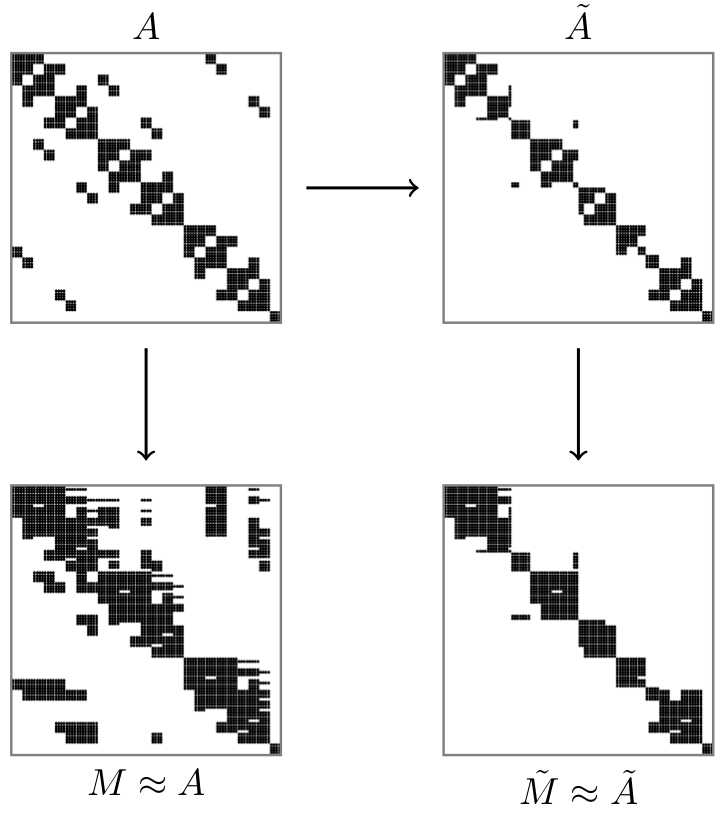
\includegraphics[width=0.5\linewidth]{combine_ad_ilu2.png}
%\caption{Determine the preconditioner~$M$ with access to all nonzero elements of Jacobian matrix~$A$. New approach: Determine the preconditioner~$\tilde M$ with access to a subset of $A$ using the sparsification operator~$\rho$. Based on Figure 4.1 from Lülfesmann~\cite{Lulfesmann2012Fap}.}%
%\label{f:luelfesmann-sparsify}%
%\end{figure}

Lülfesmann~\cite{Lulfesmann2012Fap} introduced a new approach in which the required elements of the Jacobian matrix $J$
are given in the form of the nonzero elements within $k\times k$ blocks on the main diagonal.
Then, the preconditioner is built based on these selected nonzero required elements instead of
the whole Jacobian matrix.
Building a preconditioner based on a subset of the nonzero elements is explained in~\cite{Cullum2006}.
We call these required elements \textit{initially} required elements represented by $R_i$
since they are an initial set for the further process.
Now, the coloring problem can be solved
restricted to the set of initially required nonzero elements $R_i$.

The result of a coloring algorithm groups columns and rows together.
In this process, the required elements of $J$ are always computed.
The remaining nonzero elements of $J$, which are called the nonrequired elements,
are divided into two sets of
elements: the elements which are computed and the ones which would be
eliminated. We can think of these computed nonrequired nonzero elements as byproducts
of the coloring and computing the matrix-matrix products $JV$ and $WJ$.
Since the number of colors does not change,
the idea is to add these extra byproducts also to $R_i$.
So, we call these byproduct elements the \textit{potentially}
required elements $R_p$ which are specified by
$$
R_p \subset \operatorname{pat}(J) - R_i \quad\text{so that}\quad |\Phi(R_i)| = |\Phi(R_i\cup R_p)|,
$$
where $\operatorname{pat}(J)$ represents the nonzero pattern of the Jacobian matrix $J$.

As we have discussed, an ILU preconditioner applied to $R_i$ can produce fill-in.
%Different methods can be employed to compute the preconditioner.
A subset $R_a$ of potentially required elements,
which is called the set of \textit{additionally} required elements,
is selected such that no new fill-in is generated.
These elements can be added to the
initially required elements for further computation.
The additionally required elements are formulated as follows.
$$
R_a \subset R_p \quad\text{so that}\quad SILU(R_i) \cup R_a = SILU(R_i\cup R_a),
$$
in which $SILU$ means the symbolic ILU factorization.

Now, we formulate two optimization problems in this thesis as follows.
\begin{problem}[Maximum Potentially Required Elements]
\label{p:max_pot}
%
Let $J$ be a sparse $m\times n$ Jacobian matrix with known sparsity pattern and
$R_i$ is a set of required elements.
Find a set of potentially required elements $R_p$ with maximal cardinality.
\end{problem}

\begin{problem}[Maximum Additionally Required Elements]
\label{p:max_add}
%
Let $J$ be a sparse $m\times n$ Jacobian matrix with known sparsity pattern and
$R_i$ is a set of required elements.
Find a set of additionally required elements $R_a$ with maximal cardinality.
\end{problem}
The overall approach applied to a specific problem from aerodynamics is detailed in
~\cite{cscpaper}.


\subsection{Combinatorial model}
\label{ss.comb.precond}
The bipartite graph model presented in~\defref{d.bip.graph} is
a suitable model to find new algorithms for the initially, potentially,
and additionally required elements.
Recall that each edge in the bipartite graph model is related to a nonzero element in
the matrix.
Then, given a bipartite matrix $G = (V,E)$,
three subsets $E_i, E_p, E_a\subset E$
are considered for the initially, potentially,
and additionally required elements, respectively.
Given the $k\times k$ block on the diagonal as required elements $R_i$ and the Jacobian matrix $J$,
here is a list of steps in the computation of additionally required elements
and the corresponding algorithm on the bipartite graph model.
More details can be found in~\cite{Lulfesmann2012Fap}.
\begin{itemize}
\item choose the initially required elements $R_i$.
\item setup the bipartite graph $G$ from the Jacobian matrix $J$ and the subset $E_i\subset E$ representing $R_i$.
\item compute the coloring $\Phi(E_i)$ of the bipartite graph $G$ restricted to $E_i$.
\item find the set of potentially required elements $E_p\subset E - E_i$ such that $|\Phi(E_i)| = |\Phi(E_i \cup E_p)|$.
\item find the set of additionally required elements $E_a\subset E_p$ such that $SILU(R_i) \cup R_a
    = SILU(R_i \cup R_a)$.
\end{itemize}
\coderef{code.pot.d2} and \coderef{code.pot.sb} show the algorithms to compute the
potentially required elements for the distance-$2$ coloring and star bicoloring, respectively.
In these algorithms, $N_1$ means the distance-$1$ neighbors (edges).
Given a bipartite graph $G$, the required edges $E_i$, and a distance-$2$ coloring $\Phi$,
\coderef{code.pot.d2} computes a set of potentially required elements. This algorithm
iterates over nonrequired edges ($E - E_i$) and checks if such an edge can be added to the
set of potentially required elements. Similarly, \coderef{code.pot.sb} computes
the potentially required elements when the given coloring $\phi$ is a star bicoloring.
\begin{figure}
\begin{lstlisting}[caption=Find potentially required elements for
distance-$2$ coloring (based on the algorithm 4.2 from~\cite{Lulfesmann2012Fap}).,label=code.pot.d2,mathescape]
function pot_d2_coloring($G=(V_r\cup V_c,E)$,$E_i\subseteq E$,$\phi$)
  $E_p=\emptyset$
  for $(r_i,c_j)\in E-E_i$ with $\Phi(c_j)\neq 0$
    for $c_k\in N_1(r_i,G)$ with $j\neq k$ and $(r_i,c_k)\notin E_i$
      if $\Phi(c_j) = \Phi(c_k)$
        continue with next edge $(r_i,c_j)\in E-E_i$
    $E_p = E_p \cup \{(r_i,c_j)\}$
  return $E_p$
\end{lstlisting}
\end{figure}
\begin{figure}
\begin{lstlisting}[caption=Find potentially required elements for star bicoloring (based on Algorithm 4.3 from ~\cite{Lulfesmann2012Fap}).,label=code.pot.sb,mathescape]
function pot_star_bicoloring($G=(V_r\cup V_c,E)$,$E_i\subseteq E$,$\phi$)
  $E_p = \emptyset$
  for $(r_i,c_j)\in E-E_i$ with $\Phi(r_i)\neq 0$ or $\Phi(c_j)\neq 0$
    if $\Phi(r_i) = 0$
      for $c_k\in N_1(r_i,G)$ with $j\neq k$ and $(r_i,c_k)\notin E_i$
        if $\Phi(c_j)=\Phi(c_k)$
          continue with the next edge $(r_i,c_j)\in E - E_i$

    if $\Phi(c_j) = 0$
      for $r_l\in N_1(c_j,G)$ with $j\neq l$ and $(r_l,c_j)\notin E_i$
        if $\Phi(r_i)=\Phi(r_l)$
          continue with the next edge $(r_i,c_j)\in E - E_i$

    if $\Phi(r_i) \neq 0$ and $\Phi(c_j) \neq 0$
      for $c_k\in N_1(r_i,G)$ with $i\neq k$
        for $r_l\in N_1(c_j,G)$ with $j\neq l$
          if $\Phi(c_j)=\Phi(c_k)$ and $\Phi(r_i)=\Phi(r_l)$
            continue with the next edge $(r_i,c_j)\in E - E_i$

    $E_p = E_p \cup \{(r_i,c_j)\}$
  return $E_p$
\end{lstlisting}
\end{figure}

To compute the additionally required elements, a formulation of ILU preconditioning
in the language of graphs is needed.
Hysom and Pothen~\cite{precond-pothen} introduced a graph model for the incomplete
LU factorization in which the matrix is the adjacency matrix of this graph.
It should be considered that the graph would be directed if the matrix is not symmetric.
The concept of \textit{fill path} is defined to characterize the fill-in in ILU preconditioning,
\begin{definition}[Fill path]\label{d.fill.path}
A fill path is a path $(v_i,...,v_k,...,v_j)$ with
$k<\min(i,j)$. It means the index of all the inner nodes in a given ordering of vertices
is smaller than the indices of the vertices $v_i$ and $v_j$.
\end{definition}
It follows that a matrix element $(i,j)$ is a fill-in if and only if there is a fill path between
$v_i$ and $v_j$.
In addition to the concept of fill path, another concept of fill level $l$ is needed to
formulate the level-based incomplete LU factorization~\cite{precond-pothen}.
This parameter is used to filter the generated fill-in.
This parameter is the length of the fill path.
In the level-based incomplete LU factorization, the generated fill-in is allowed
to be considered only up to the level $l$.
We fix this level parameter to $2$ throughout this thesis.

\begin{figure}
\begin{lstlisting}[caption=Find additionally required elements (based on Algorithm 4.5 from ~\cite{Lulfesmann2012Fap}).,
label=code.add,mathescape]
function add($G=(V_r\cup V_c,E)$,$E_i\subseteq E$,$E_p$,$E_F$)
  $E_a = \emptyset$
  do
    for $(r_i,c_j)\in E_p$
      if $i > j$
        for $c_l\in N_1(r_j,G[E_i\cup (E_F\cup E_a)])$ with $l > j$
          if $(r_i,c_l)\notin E_i\cup (E_F\cup E_a)$
            continue with next edge $(r_i,c_j)\in E_p$
      else if $i \leq j$
        for $r_k\in N_1(c_i,G[E_i\cup (E_F\cup E_a)])$ with $k > i$
          if $(r_k,c_j)\notin E_i\cup (E_F\cup E_a)$
            continue with next edge $(r_i,c_j)\in E_p$
      $E_a = E_a \cup \{(r_i,c_j)\}$
      $E_p = E_p - \{(r_i,c_j)\}$
  while $|E_a|$ is increased in the last iteration
  return $E_a$
\end{lstlisting}
\end{figure}
Lülfesmann~\cite{Lulfesmann2012Fap} adapted a
corresponding bipartite graph model for ILU preconditioning.
The concept of fill path is also redefined for the bipartite graph model
in which a path is replaced by a distance-$2$ path.
\begin{definition}[Fill path in bipartite graph]\label{d.fill.path.bipartite}
A path $(r_i,c_k,r_k,c_l,r_l,...,c_j)$ in the bipartite graph model starting
from a row vertex is a fill path
if and only if all vertices between $r_i$ and $c_j$ have a lower index than $i$
and $j$.
\end{definition}
Again, it follows that
there is a fill-in $(i,j)$ in the matrix if and only if there is a
fill path between $r_i$ and $c_j$ in the corresponding bipartite graph.

Based on the bipartite graph models for coloring and the ILU preconditioning,
Lülfesmann~\cite{Lulfesmann2012Fap} proposed two algorithms to compute the additionally required elements: conservative and sophisticated.
We consider the sophisticated algorithm shown in \coderef{code.add}
to compute the additionally required elements
throughout this thesis. This algorithm looks at each potentially required edge.
If it is possible that a fill path generated by adding this edge,
the edge is not considered for the set of additionally required edges.
In this sophisticated approach, the algorithm iterates once again over
all potentially required elements. This process is repeated until
no new additionally required edges are found.

%%%%%%%%%%%%%%%%%%%%%%%%%%%%%%%%%%%%%%%%%%%%%%%%%%%%%%%%%%%%%%%%%%%%%%%%%%%%%%%%%%%%%%%%%%%%%%%%%%%%%%%%%%%%%%%%%%%%%%%%%%%%%%%%
%%%% PRECONDITIONING AND COLORING
%%%%%%%%%%%%%%%%%%%%%%%%%%%%%%%%%%%%%%%%%%%%%%%%%%%%%%%%%%%%%%%%%%%%%%%%%%%%%%%%%%%%%%%%%%%%%%%%%%%%%%%%%%%%%%%%%%%%%%%%%%%%%%%%
\chapter{New coloring heuristics}
\label{package}
Karp~\cite{karp:1972} proves that the graph coloring problem is NP-complete for general graphs.
Hence, various coloring heuristics are studied throughout the years with a polynomial complexity.
Greedy coloring is a widely used heuristic which has a low computational complexity
and computes a \textit{reasonable} coloring (see~\cite{spaa14}).
The greedy coloring algorithm for the restricted distance-$2$ coloring
is given in \coderef{code.greedy} which is adapted from Lülfesmann~\cite{Lulfesmann2012Fap}.
The computed coloring $\Phi:V_c\to\{1,2,...,p\}$ on the vertex set $V_c=\{1,2,...,n\}$
is restricted to the initially required edges $E_i$.
All arrays in all algorithms, like $forbiddenColors$,
implemented in this thesis start with the index $0$.
The assignment $forbiddenColors[c]=v$ means the vertex $v$ can not be colored
by the color $c$. Since this algorithm does not consider the color $0$,
the element $forbiddenColors[0]$ is ignored in line 7 of \coderef{code.greedy}.

In this algorithm, the function $N_2(v,E_i)$ finds all distance-$2$ neighbors
of $v$ restricted to the set of initially required edges $E_i$.
More clearly, the function $N_2(v,E_i)$ computes
all vertices on all paths of length $2$ from the vertex $v$
such that at least one edge of such a path is in the set $E_i$,
$$
N_2(v,E_i)=\{ z\in V: \text{ there is a path } (v,w,z) \text{ with } (v,w)\in E_i
\text{ or } (w,z)\in E_i \text{ or both.}\}
$$
To color a vertex $v$ we iterate over all its distance-$2$ neighbors in $N_2(v,E_i)$ which are
already colored. Remember that these assigned colors can not be used to color the vertex $v$.
After collecting all these forbidden colors, we assign to $v$ the color with the smallest index different from
these forbidden colors.
It follows that the computational complexity of this algorithm is $\mathcal{O}(n \Delta^2)$ in which $n$
and $\Delta$ are the number of vertices and the maximum vertex degree, respectively.
Recall from the last chapter that the Jacobian matrices are sparse. Therefore, $n$ is large and $\Delta$ and $\Delta^2$
are relatively small.

\begin{figure}
\begin{lstlisting}[caption=The greedy algorithm for
the distance-$2$ coloring restricted to the edge set $E_i$
for columns.,label=code.greedy,mathescape]
function d2_color($G=(V_r\cup V_c,E)$,$E_i\subseteq E$)
  $\Phi\leftarrow [0\ldots 0]$
  $forbiddenColors\leftarrow [0\ldots 0]$
  for $v\in V_c$ with $\exists r\in V_r: (v,r) \in E_i$
    for $n\in N_2(v,E_i)$ with $\Phi(n) \neq 0$
        $forbiddenColors[\Phi(n)] = v$
    $\Phi(v) = \min \{ a>0:forbiddenColors[a]\neq v\}$
  return $\Phi$
\end{lstlisting}
\end{figure}

In this algorithm, vertices are colored one at a time.
Therefore, the vertex ordering plays a major role in the greedy algorithm.
Hence, there are many publications on how to choose
a suitable ordering for a serial or parallel version of
coloring~\cite{ordering1,ordering2}.
Various orderings are studied for coloring heuristics
throughout the years. Here are some orderings for coloring which are applied before doing the coloring:
the largest-first ordering (LFO)~\cite{LFO}, the incidence-degree ordering (IDO)~\cite{IDO},
the saturation-degree ordering (SDO)~\cite{ordering2}, and the smallest-last ordering (SLO)~\cite{ordering1}.

This chapter is structured as follows.
We modify the greedy algorithm in \secref{s.max.pot.req}
such that the number of potentially and additionally required elements are increased.
Later, we discuss a better heuristic for
the special case of coloring restricted to a diagonal in~\secref{s.part.color.diag}.
%We sketch the first ideas toward a new heuristic based on the exact coloring in small
%subgraphs in~\secref{s.exact}.
Finally, we introduce our computational package \textit{PreCol}
in~\secref{s.extend} that computes the
unidirectional and bidirectional restricted colorings with different algorithms
as well as the ILU preconditioning.

Throughout this chapter, the numerical experiments are carried out using
the matrices in Table~\ref{florida.mats} from the Florida sparse matrix collection~\cite{florida.matrices}.
\begin{table}
\centering
\begin{tabular}{|c|c|c|c|}
\hline
Matrix & Size & Nonzeros & Symmetric\\\hline
\textit{steam1.mtx} & $240\times 240$ & $2248$ & false\\\hline
\textit{steam2.mtx} & $600\times 600$ & $5660$ & false\\\hline
\textit{685\_bus.mtx} & $685\times 685$ & $3249$ & true\\\hline
\textit{nos3.mtx} & $960\times 960$ & $15844$ & true\\\hline
\textit{ex7.mtx} & $1633\times 1633$ & $46626$ & false\\\hline
\textit{ex33.mtx} & $1733\times 1733$ & $22189$ & true\\\hline
\textit{orani678.mtx} & $2529\times 2529$ & $90158$ & false\\\hline
\textit{cavity16.mtx} & $4562\times 4562$ & $137887$ & false\\\hline
\textit{crystm01.mtx} & $4875\times 4875$ & $105339$ & true\\\hline
\textit{rajat01.mtx} & $6833\times 6833$ & $43250$ & false\\\hline
\textit{gyro\_m.mtx} & $17361\times 17361$ & $340431$ & true\\\hline
\textit{ford2.mtx} & $100196\times 100196$ & $544688$ & true\\\hline
\textit{cage3.mtx} & $5\times 5$ & $19$ & false\\\hline
\textit{cage4.mtx} & $9\times 9$ & $49$ & false\\\hline
\textit{cage5.mtx} & $37\times 37$ & $233$ & false\\\hline
\textit{cage6.mtx} & $93\times 93$ & $785$ & false\\\hline
\textit{cage7.mtx} & $340\times 340$ & $3084$ & false\\\hline
\textit{cage8.mtx} & $1015\times 1015$ & $11003$ & false\\\hline
\textit{cage9.mtx} & $3534\times 3534$ & $41594$ & false\\\hline
\textit{cage10.mtx} & $11397\times 11397$ & $150645$ & false\\\hline
\textit{cage12.mtx} & $130228\times 130228$ & $2032536$ & false\\\hline
\end{tabular}
\caption{
Throughout this chapter, the numerical experiments are carried out using
these matrices from the Florida sparse matrix collection.}
\label{florida.mats}
\end{table}

%%%%%%%%%%%%%%%%%%%%%%%%%%%%%%%%%%%%%%%%%%%%%%%%%%%%%%%%%%%%%%%%%%%%%%%%%%%%%
\section{Maximizing the set of additionally required elements}
\label{s.max.pot.req}
%%%%%%%%%%%%%%%%%%%%%%%%%%%%%%%%%%%%%%%%%%%%%%%%%%%%%%%%%%%%%%%%%%%%%%%%%%%%%
Here, our focus is to solve the optimization Problems~\ref{p:max_pot} and~\ref{p:max_add}.
As we have discussed, there are nonrequired nonzero elements
which are also computed as a by-product of the computation of required elements.
The nonrequired elements have a major effect on
the determination of potentially required elements
and additionally required elements.
The following example illustrates that
a modified coloring can increase the number of nonrequired elements
which are determined.
\newcolumntype{r}{>{\columncolor{red!60}}c}
\newcolumntype{b}{>{\columncolor{blue!60}}c}
\begin{equation}
\left(\begin{array}{rrb}
* & * & *\\
0 & r & r \\
* & 0 & *
\end{array}\right)
\qquad
\left(\begin{array}{rbr}
* & * & *\\
0 & r & r \\
* & 0 & *
\end{array}\right)
\label{twocolorings}
\end{equation}
Here, the symbol $r$ stands for a required element,
the symbol \textit{$*$} stands for other nonzero elements (the nonrequired elements),
and the number $0$ denotes a zero element.

If the first and second columns get the same color as given in the left matrix,
we will get the nonzero at position $(3,1)$ as a by-product.
However, there are certain degrees of freedom. In
this example, one could also assign the same color to columns $1$ and
$3$ as illustrated in the right matrix
in which no nonzero element in the last row will be computed
as a by-product. This idea leads to the problem of maximizing
the number of nonrequired nonzero elements that are computed as a by-product.
Here, we introduce a new heuristic which increases the number of determined nonrequired elements
while the number of colors remains almost the same.

\subsection{Restricted distance-$2$ coloring}
Our goal here is to increase the number of potentially and additionally required elements.
Given a bipartite graph $G=(V_c\cup V_r,E)$ and a vertex $v\in V_c$,
we define a function $\nreq_v:S\subseteq V_c\rightarrow \mathbb{N}$.
The function $\nreq_v(w)$ computes the number of nonrequired elements
that are actually determined by
the linear combination of the columns corresponding to the vertices $v$ and $w$.
We call these elements the determined nonrequired elements.
\begin{figure}
\begin{lstlisting}[caption=New coloring heuristic for distance-$2$ coloring
considering the nonrequired elements.,label=code.new.d2.nreq,mathescape]
function d2_color_nreq($G=(V_r\cup V_c,E)$,$E_i\subseteq E$)
  $\Phi\leftarrow [0\ldots 0]$
  $forbiddenColors\leftarrow [0\ldots 0]$
  for $v\in V_c$ with $\exists r\in V_r: (v,r) \in E_i$ and $\Phi(v)=0$
    for $n\in N_2(v,E_i)$ with $\Phi(n) \neq 0$
      $forbiddenColors[\Phi(n)] = v$
    $\Phi(v) = \min \{ a>0:forbiddenColors[a]\neq v\}$

    $I_v=\{z\in V_c: z\neq v\text{ and }z\notin N_2(v) \text{ and } \Phi(z) = 0 \}$
    if $I_v\neq\emptyset$
      $maxs = \argmax_{x\in I_v} \nreq_v (x)$
      $\Phi(maxs[0]) = \Phi(v)$
  return $\Phi$
\end{lstlisting}
\end{figure}
Here, we focus on the unidirectional compression for columns represented by $V_c$.
However, an analogous discussion holds for the unidirectional compression for rows.

We modify the greedy algorithm  presented in \coderef{code.greedy} as follows.
%Our approach in this new coloring algorithm is based on finding independent sets.
%In a general graph $G=(V,E)$, a subset of the vertices $I\subseteq V$ is
%called an independent set~\cite{bondy2008graph}
%if there is no edge between any of its vertices,
%$$\forall u,v\in I: (u,v)\notin E.$$
%In the bipartite graph model of \defref{d.bip.graph},
%we need to change the definition of an independent set using the distance-$2$ neighbors as follows.
%$$\forall u,v\in I: u\notin N_2(v).$$
%Also, we represent an independent set containing the vertex $v$ by $I_v$.
%This set represents the vertices that can have the same colors as the vertex $v$.
%Here, we use this adapted definition for simplicity.
%Other definitions are possible using $N_2(v,E_i)$ which
%may result in a more efficient heuristic.
For this new heuristic, we define two operators.
Given a function $f:A\rightarrow B$ and a subset $S\subseteq A$
the operators $\argmax$ and $\argmin$ are defined as,
\begin{equation*}
\begin{split}
\argmax_{x\in S} f(x) &= \{ x \mid \forall y\in S: f(y) \leq f(x)\}, \\
\argmin_{x\in S} f(x) &= \{ x \mid \forall y\in S: f(y) \geq f(x)\}.
\end{split}
\end{equation*}

\coderef{code.new.d2.nreq} shows this new heuristic.
In this algorithm, we iterate over all uncolored vertices.
First, we color the vertex $v$ with a color different form
its distance-$2$ neighbors restricted to $E_i$ like the previous greedy coloring.
Note, however, that there is an additional condition which
ensures that the vertex $v$ has not been previously colored.
After the coloring of $v$, \coderef{code.new.d2.nreq} finds the set $I_v$
representing the uncolored vertices that can have the same color as the vertex $v$.
Additionally, we compute $\nreq_v(x)$ for each vertex $x\in I_v$
and color a vertex $w\neq x$ with the same color as $v$
if $w$ leads to the maximum value of $\nreq_v(w)$.
The time complexity of this new heuristic is estimated as follows.
The outer loop at most consists of $n$ vertices.
For a vertex $v$, the complexity of coloring in line 5 to 7 is $\mathcal{O}(\Delta^2)$ as
in \coderef{code.greedy}. The set $I_v$ is computed in $\mathcal{O}(n)$.
Since the computation of $\nreq_v(w)$ is $\mathcal{O}(n)$, the computation of
the set $maxs$ is $\mathcal{O}(n^2)$. Thus, the general complexity is given by $\mathcal{O}(n^3)$.

Although we color a vertex $v$ and another vertex $u\in I_v$ in each iteration
it does not always mean that the coloring is valid. Consider the Jacobian and
its bipartite graph model in \figref{twocolorings2} where the required edges are the bold edges in the graph.
%\begin{equation}
%\left(\begin{array}{cccc}
%r & 0 & 0 & 0  \\
%0 & 0 & r & 0 \\
%0 & * & * & 0 \\
%0 & r & 0 & r \\
%\end{array}\right)
%\label{twocolorings2}
%\end{equation}
\begin{figure}
\centering
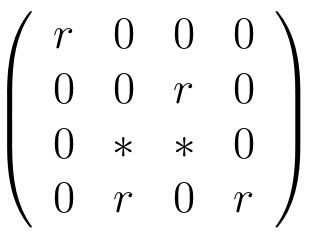
\includegraphics[width=0.25\linewidth]{example_matrix}
\qquad
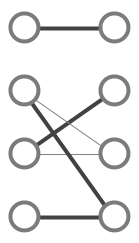
\includegraphics[width=0.12\linewidth]{example_bipartite}
\caption{An example of a Jacobian and its bipartite graph model
in which \coderef{code.new.d2.nreq} does not generate a valid coloring.}
\label{twocolorings2}
\end{figure}

Here, we assume that the outer loop is executed in a natural ordering corresponding to iterate over
the columns of the Jacobian from left to right.
After the first vertex $v_1$ corresponding to the first column is given some color,
the set $I_v$ consists of the columns $2$, $3$, and $4$. Since all these three columns
can be compressed with the first column, the function $\nreq_{v_1}(x)$ is given by the number of
nonrequired elements in a column corresponding to $x$. Thus, the values of $\nreq_{v_1}(x)$
for the columns $2$, $3$, and $4$ are $1$, $1$, $0$, correspondingly.
Therefore, the first and the second column are colored identically.
In the next iteration of the outer loop, the third column is then colored with the same color as the first
column since the vertex $v_3$ corresponding to the third column does not have any distance-$2$ neighbors
restricted to $E_i$. Thus, the array $forbiddenColors$ is not changed in this iteration.
So, the colors of first three columns are the same.
Now, the set $I_{v_3}$ contains the vertex $v_4$ corresponding to the
fourth column since the others are already colored. Therefore, the fourth column gets the color of
the third column. However, this is not a valid coloring since the fourth and second columns can not be compressed.
\begin{figure}
\begin{lstlisting}[
label=consistency,caption=A function which checks the validation of the coloring.,mathescape]
function is_valid($G=(V_r\cup V_c,E)$,$E_i\subseteq E$)
    for $v \in V_c$ and $n \in N_2(v,E_i)$
      if $\Phi(n) = \Phi(v)$
        return false
  return true
\end{lstlisting}
\end{figure}
Considering this problem, we check if the coloring is valid at the end of the algorithm
by the function given in \coderef{consistency}.
An observation is that the coloring is valid for all the matrices that are mentioned in this
thesis.

Table~\ref{mats.pot.add.gr.vs.nreq} presents the number of potentially
and additionally required elements computed
by \coderef{code.greedy} and \coderef{code.new.d2.nreq}
and for different orderings for coloring.
Table~\ref{mats.pot.add.gr.vs.nreq} (Top), (Middle), and (Bottom) are
the results for the natural ordering, the LFO ordering, and the SLO ordering, respectively.
The size of the diagonal blocks is fixed to $10$.
In these tables, the numbers of both potentially and additionally required elements
tend to increase in the new proposed \coderef{code.new.d2.nreq} regardless of the ordering.
An observation is that, for the matrix $pesa.mtx$ with the ordering LFO,
the number of potentially required elements decreases
while the number of additionally required elements increases. Also,
both the numbers of potentially and additionally required elements
decrease in \coderef{code.new.d2.nreq} for \textit{ex7.mtx} and for all orderings.

\begin{table}
\centering
\begin{tabular}{|c|c|c|c|c|}
\hline
Matrix (NAT) & \multicolumn{2}{c|}{$|R_p|$} & \multicolumn{2}{c|}{$|R_a|$}\\\hline
{} & \coderef{code.greedy} & \coderef{code.new.d2.nreq} & \coderef{code.greedy} & \coderef{code.new.d2.nreq}\\\hline
\textit{steam1.mtx} & $64$ & $786$ & $64$ & $630$ \\\hline
\textit{steam2.mtx} & $240$ & $1880$ & $240$ & $1400$ \\\hline
\textit{nos3.mtx} & $1638$ & $6756$ & $1106$ & $4296$ \\\hline
\textit{crystm01.mtx} & $17822$ & $47556$ & $10388$ & $28318$ \\\hline
\textit{ex7.mtx} & $38554$ & $34954$ & $29174$ & $25054$ \\\hline
\textit{ex33.mtx} & $7408$ & $8934$ & $4920$ & $5572$ \\\hline
\textit{coater1.mtx} & $11722$ & $11558$ & $7684$ & $7448$ \\\hline
\textit{pesa.mtx} & $36972$ & $41154$ & $31010$ & $33094$ \\\hline
\end{tabular}
\vspace*{1cm}\newline
\begin{tabular}{|c|c|c|c|c|}
\hline
Matrix (LFO) & \multicolumn{2}{c|}{$|R_p|$} & \multicolumn{2}{c|}{$|R_a|$}\\\hline
{} & \coderef{code.greedy} & \coderef{code.new.d2.nreq} & \coderef{code.greedy} & \coderef{code.new.d2.nreq}\\\hline
\textit{steam1.mtx} & $64$ & $1048$ & $64$ & $666$ \\\hline
\textit{steam2.mtx} & $240$ & $2624$ & $240$ & $1248$ \\\hline
\textit{nos3.mtx} & $1880$ & $6882$ & $1246$ & $4442$ \\\hline
\textit{crystm01.mtx} & $20326$ & $36634$ & $12256$ & $21194$ \\\hline
\textit{ex7.mtx} & $37080$ & $33426$ & $28904$ & $24060$ \\\hline
\textit{ex33.mtx} & $10574$ & $10564$ & $7170$ & $6888$ \\\hline
\textit{coater1.mtx} & $11312$ & $11512$ & $7410$ & $7536$ \\\hline
\textit{pesa.mtx} & $42490$ & $41676$ & $31790$ & $31884$ \\\hline
\end{tabular}
\vspace*{1cm}\newline
\begin{tabular}{|c|c|c|c|c|}
\hline
Matrix (SLO) & \multicolumn{2}{c|}{$|R_p|$} & \multicolumn{2}{c|}{$|R_a|$}\\\hline
{} & \coderef{code.greedy} & \coderef{code.new.d2.nreq} & \coderef{code.greedy} & \coderef{code.new.d2.nreq}\\\hline
\textit{steam1.mtx} & $64$ & $1294$ & $64$ & $754$ \\\hline
\textit{steam2.mtx} & $240$ & $3192$ & $240$ & $1912$ \\\hline
\textit{nos3.mtx} & $1682$ & $6772$ & $1132$ & $4382$ \\\hline
\textit{crystm01.mtx} & $24478$ & $45166$ & $14252$ & $26782$ \\\hline
\textit{ex7.mtx} & $36486$ & $34448$ & $27044$ & $24164$ \\\hline
\textit{ex33.mtx} & $8024$ & $10754$ & $5186$ & $7138$ \\\hline
\textit{coater1.mtx} & $10476$ & $11702$ & $7004$ & $7878$ \\\hline
\textit{pesa.mtx} & $39606$ & $44624$ & $29034$ & $34044$ \\\hline
\end{tabular}
\caption{The comparison between the number of potentially and additionally required
elements computed with \coderef{code.greedy} and \coderef{code.new.d2.nreq}.
The block size is fixed to $10$. The orderings for coloring are (Top) the natural ordering,
(Middle) LFO, and (Bottom) SLO.}
\label{mats.pot.add.gr.vs.nreq}
\end{table}


Now, we compare the results by changing the block size varying from $1$ to $70$.
We compute \coderef{code.greedy} and \coderef{code.new.d2.nreq} for the matrices \textit{ex33}
and \textit{crystm01} with the three different orderings: the natural ordering, the LFO ordering,
and the SLO ordering. Additionally, we compute the number of colors in each case too.
All figures are illustrated in \appref{app.compare.alg31.alg32}.
An observation is that the behavior of the figures of the potentially required elements and
the additionally required elements is similar. Hence, we consider only the additionally
required elements for $ex33$ now.
The number of additionally required elements computed by \coderef{code.new.d2.nreq} with the ordering SLO
is overall larger than \coderef{code.greedy} (see \figref{ex33_alg31_alg32_bls_slo_add}).
The number of colors remains almost the same for the both colorings
(see \figref{ex33_alg31_alg32_bls_slo_cols}).
Here, \coderef{code.new.d2.nreq} leads to a larger number of colors compared to \coderef{code.greedy}.
However, there are also orderings where \coderef{code.new.d2.nreq} is not superior for all block sizes in terms of
the number of additionally required elements.
For example, \figref{ex33_alg31_alg32_bls_nat_add} shows the number of additionally required elements
for the natural ordering.
Here, \coderef{code.new.d2.nreq} tends to perform better for smaller block sizes up to around $40$.
However, for larger block sizes, \coderef{code.greedy} tends to produce slightly more additionally required elements.
(see \figref{ex33_alg31_alg32_bls_nat_cols}).
%The number of colors in~\figref{bls_cols_ex33_without_alpha} for the greedy coloring
%is the minimum value between different orderings \textit{LFO}, \textit{SLO}, and \textit{IDO}.

\begin{figure}
\centering
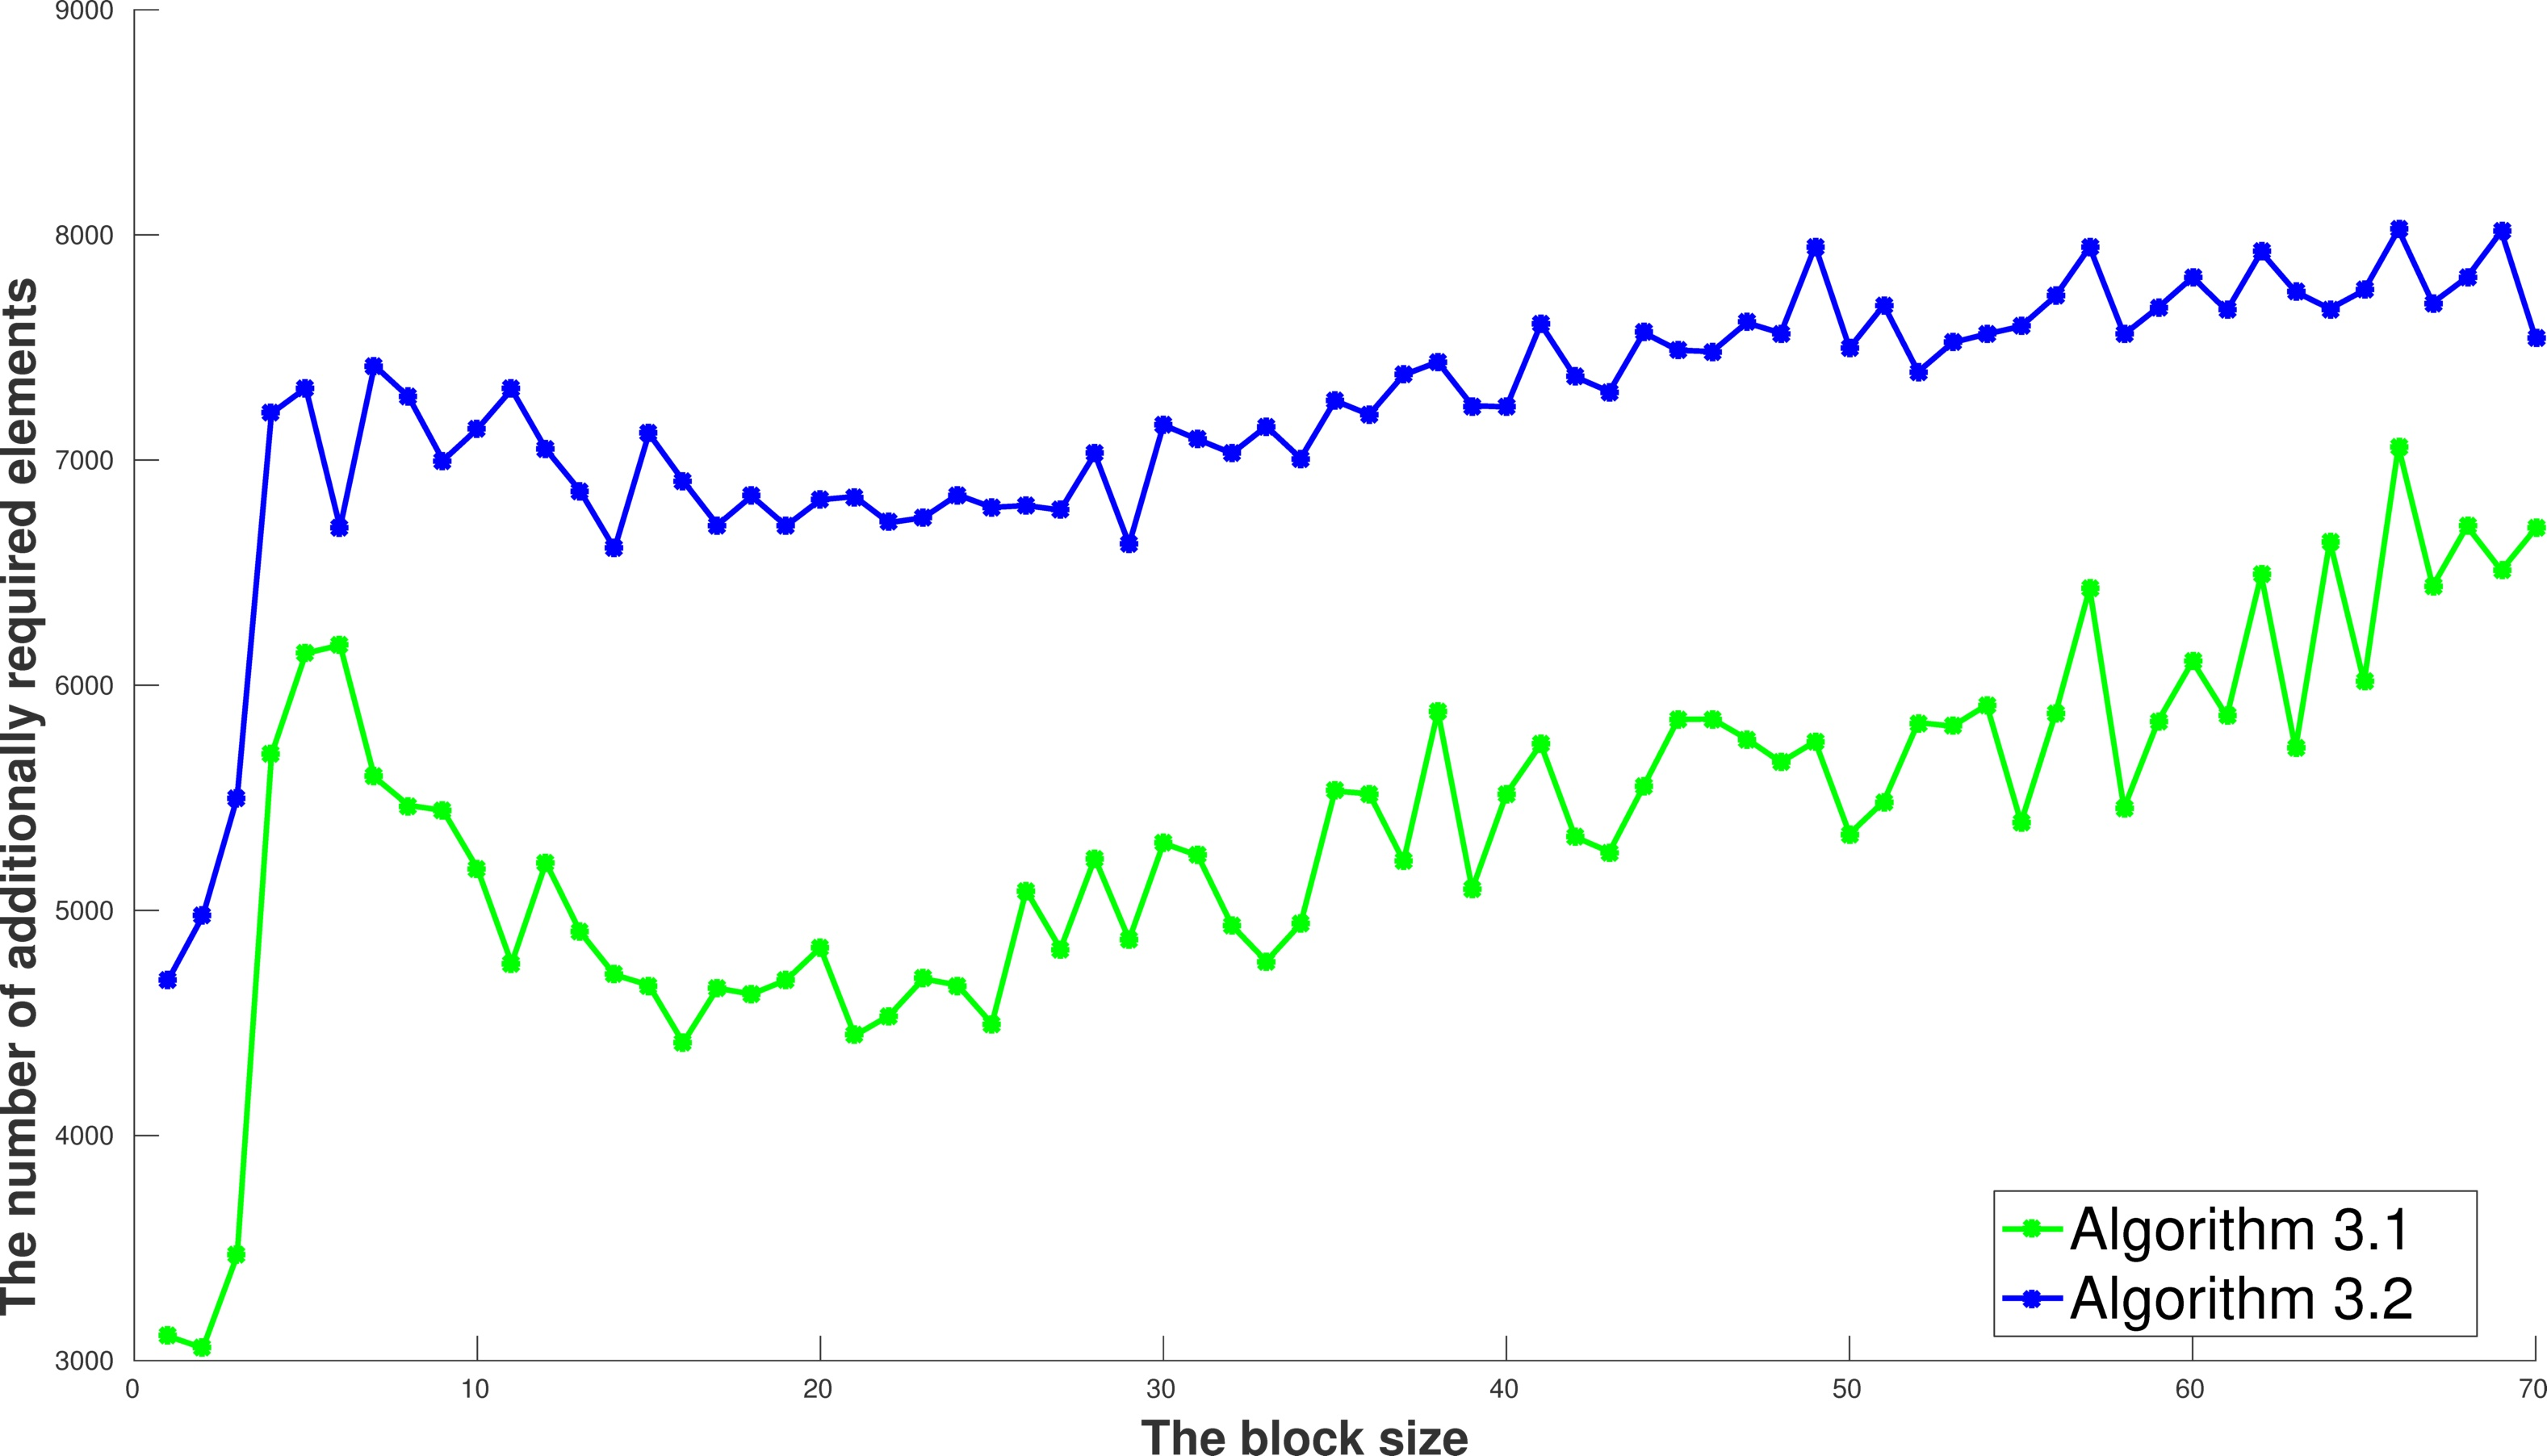
\includegraphics[width=0.9\linewidth]{ex33_alg31_alg32_bls_slo_add}
\caption{
The number of additionally required elements computed by
\coderef{code.new.d2.nreq} with the SLO ordering
compared with \coderef{code.greedy}.
The computation is carried out on the matrix \textit{ex33}. }
\label{ex33_alg31_alg32_bls_slo_add}
\end{figure}

\begin{figure}
\centering
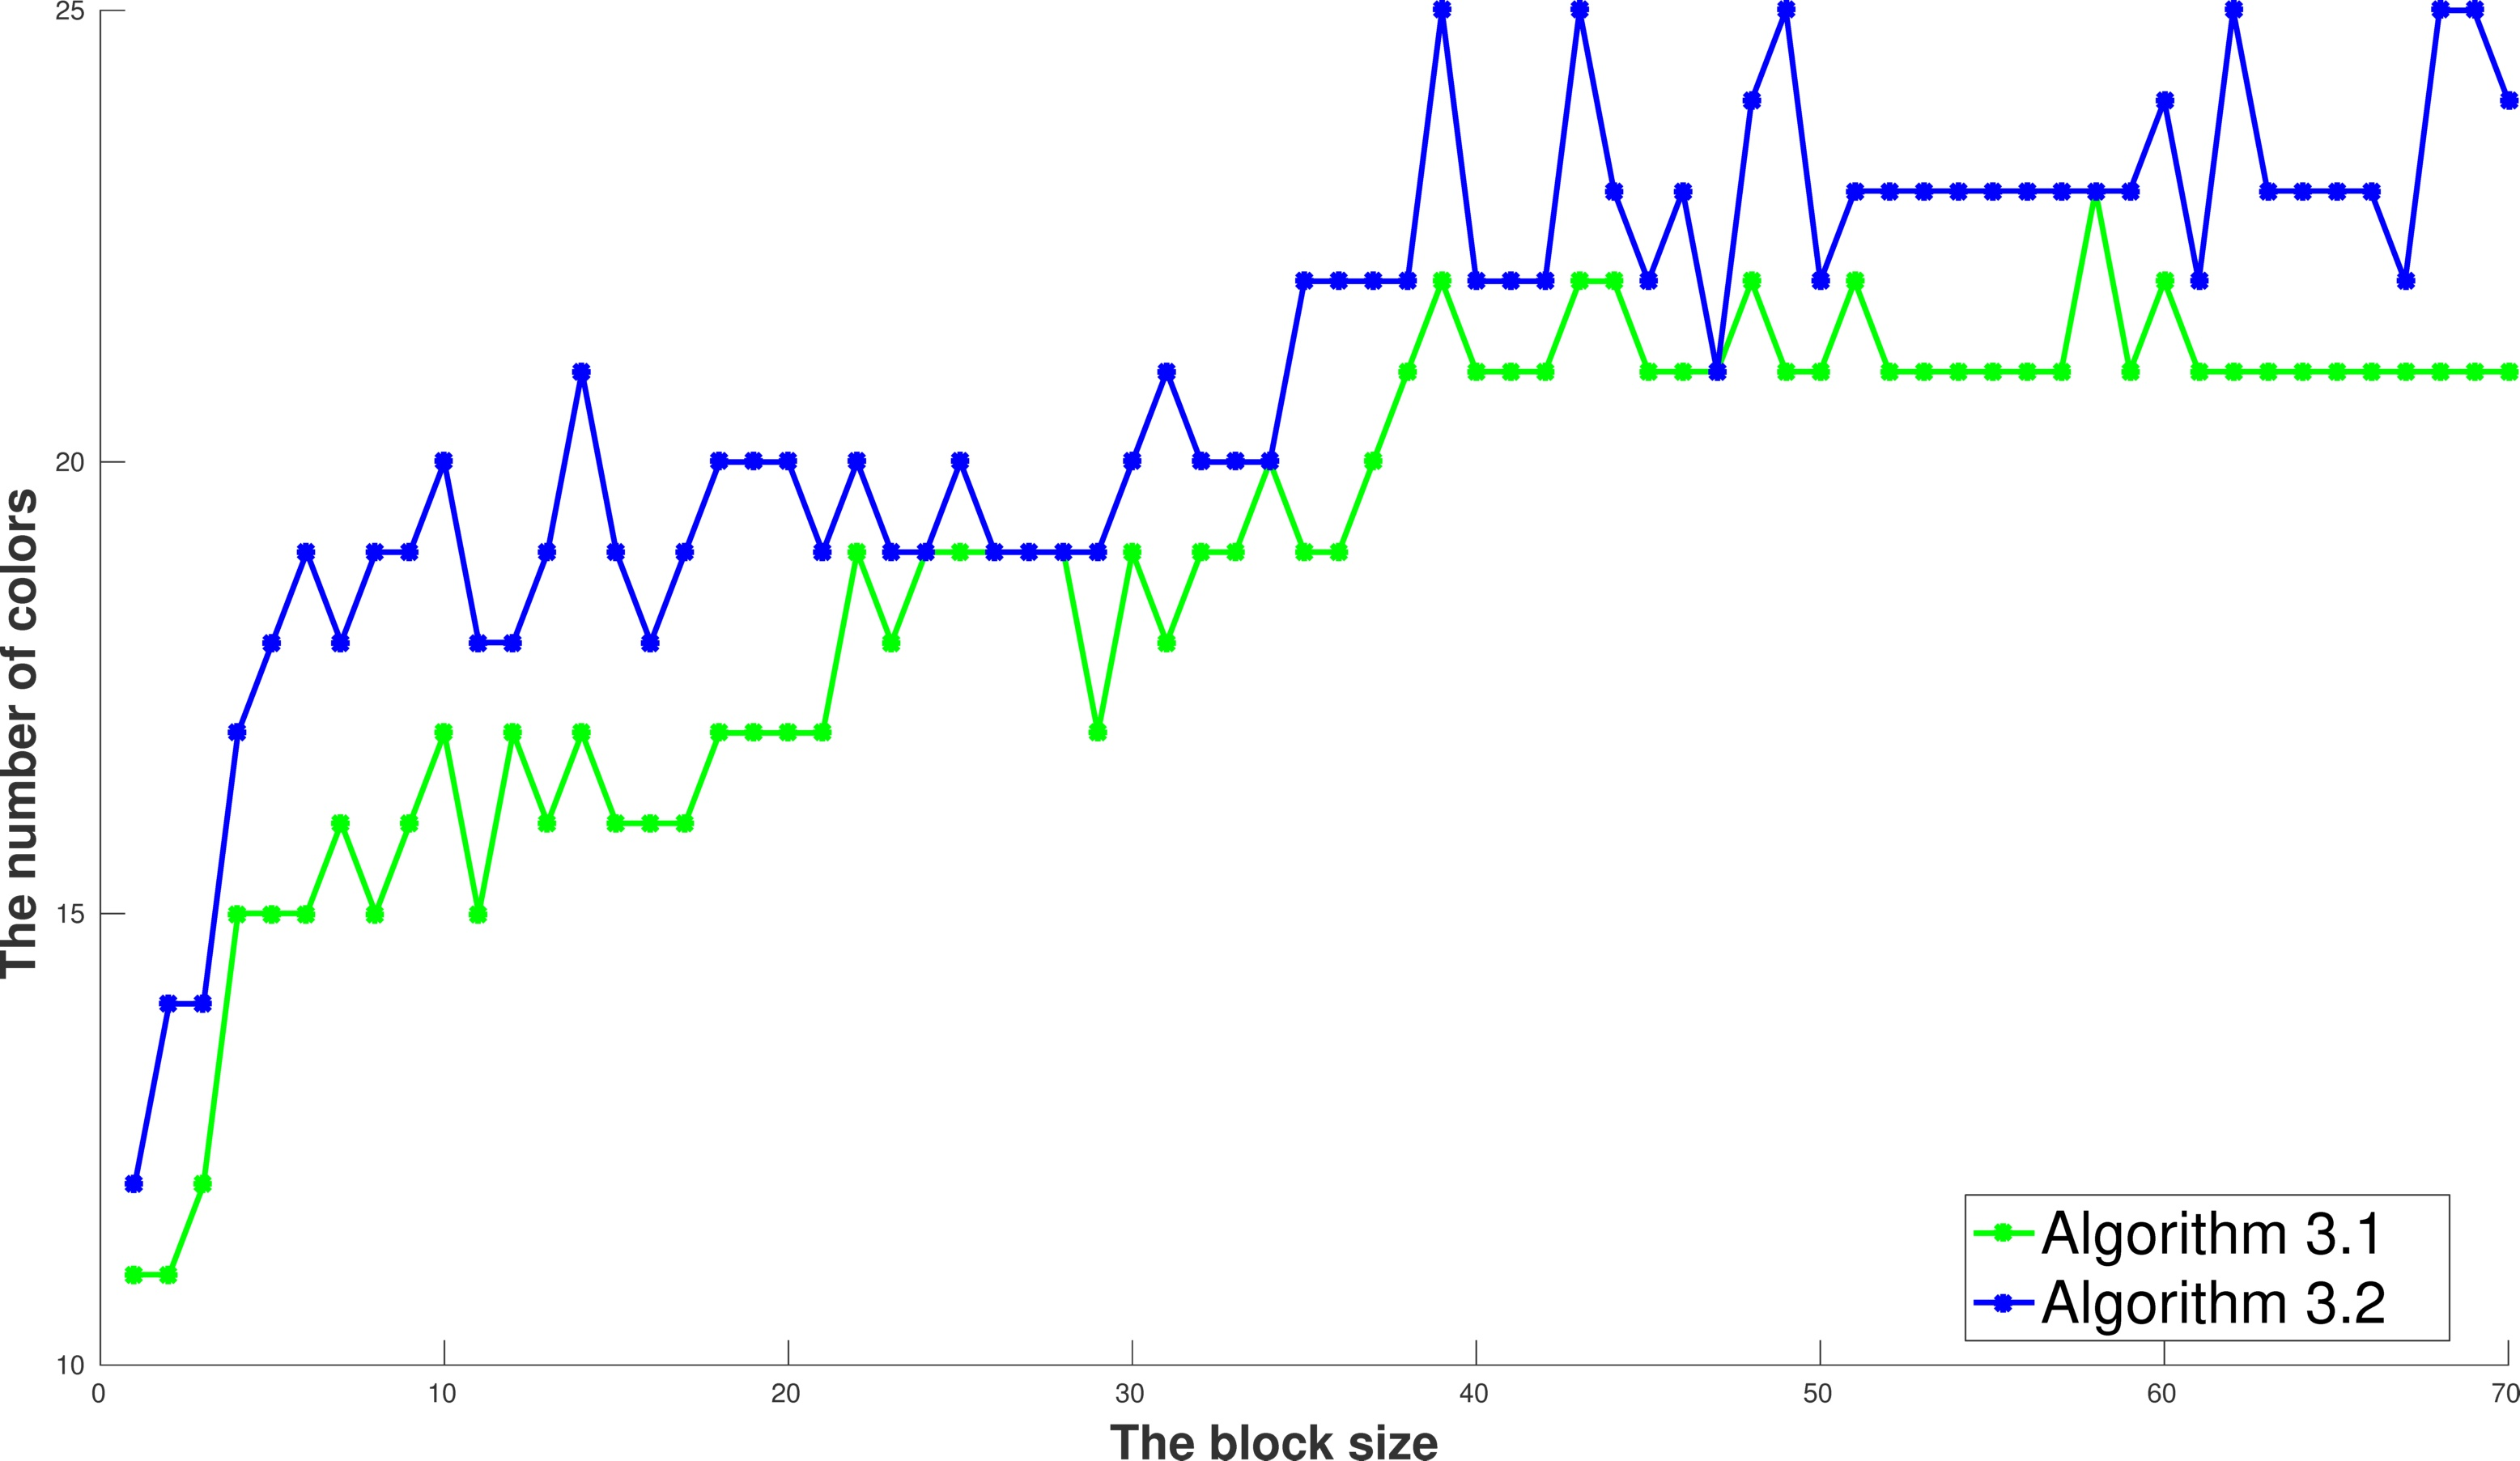
\includegraphics[width=0.9\linewidth]{ex33_alg31_alg32_bls_slo_cols}
\caption{The number of colors computed by \coderef{code.new.d2.nreq} with the SLO ordering
compared with \coderef{code.greedy}.
The computation is carried out on the matrix \textit{ex33}.}
\label{ex33_alg31_alg32_bls_slo_cols}
\end{figure}

\begin{figure}
\centering
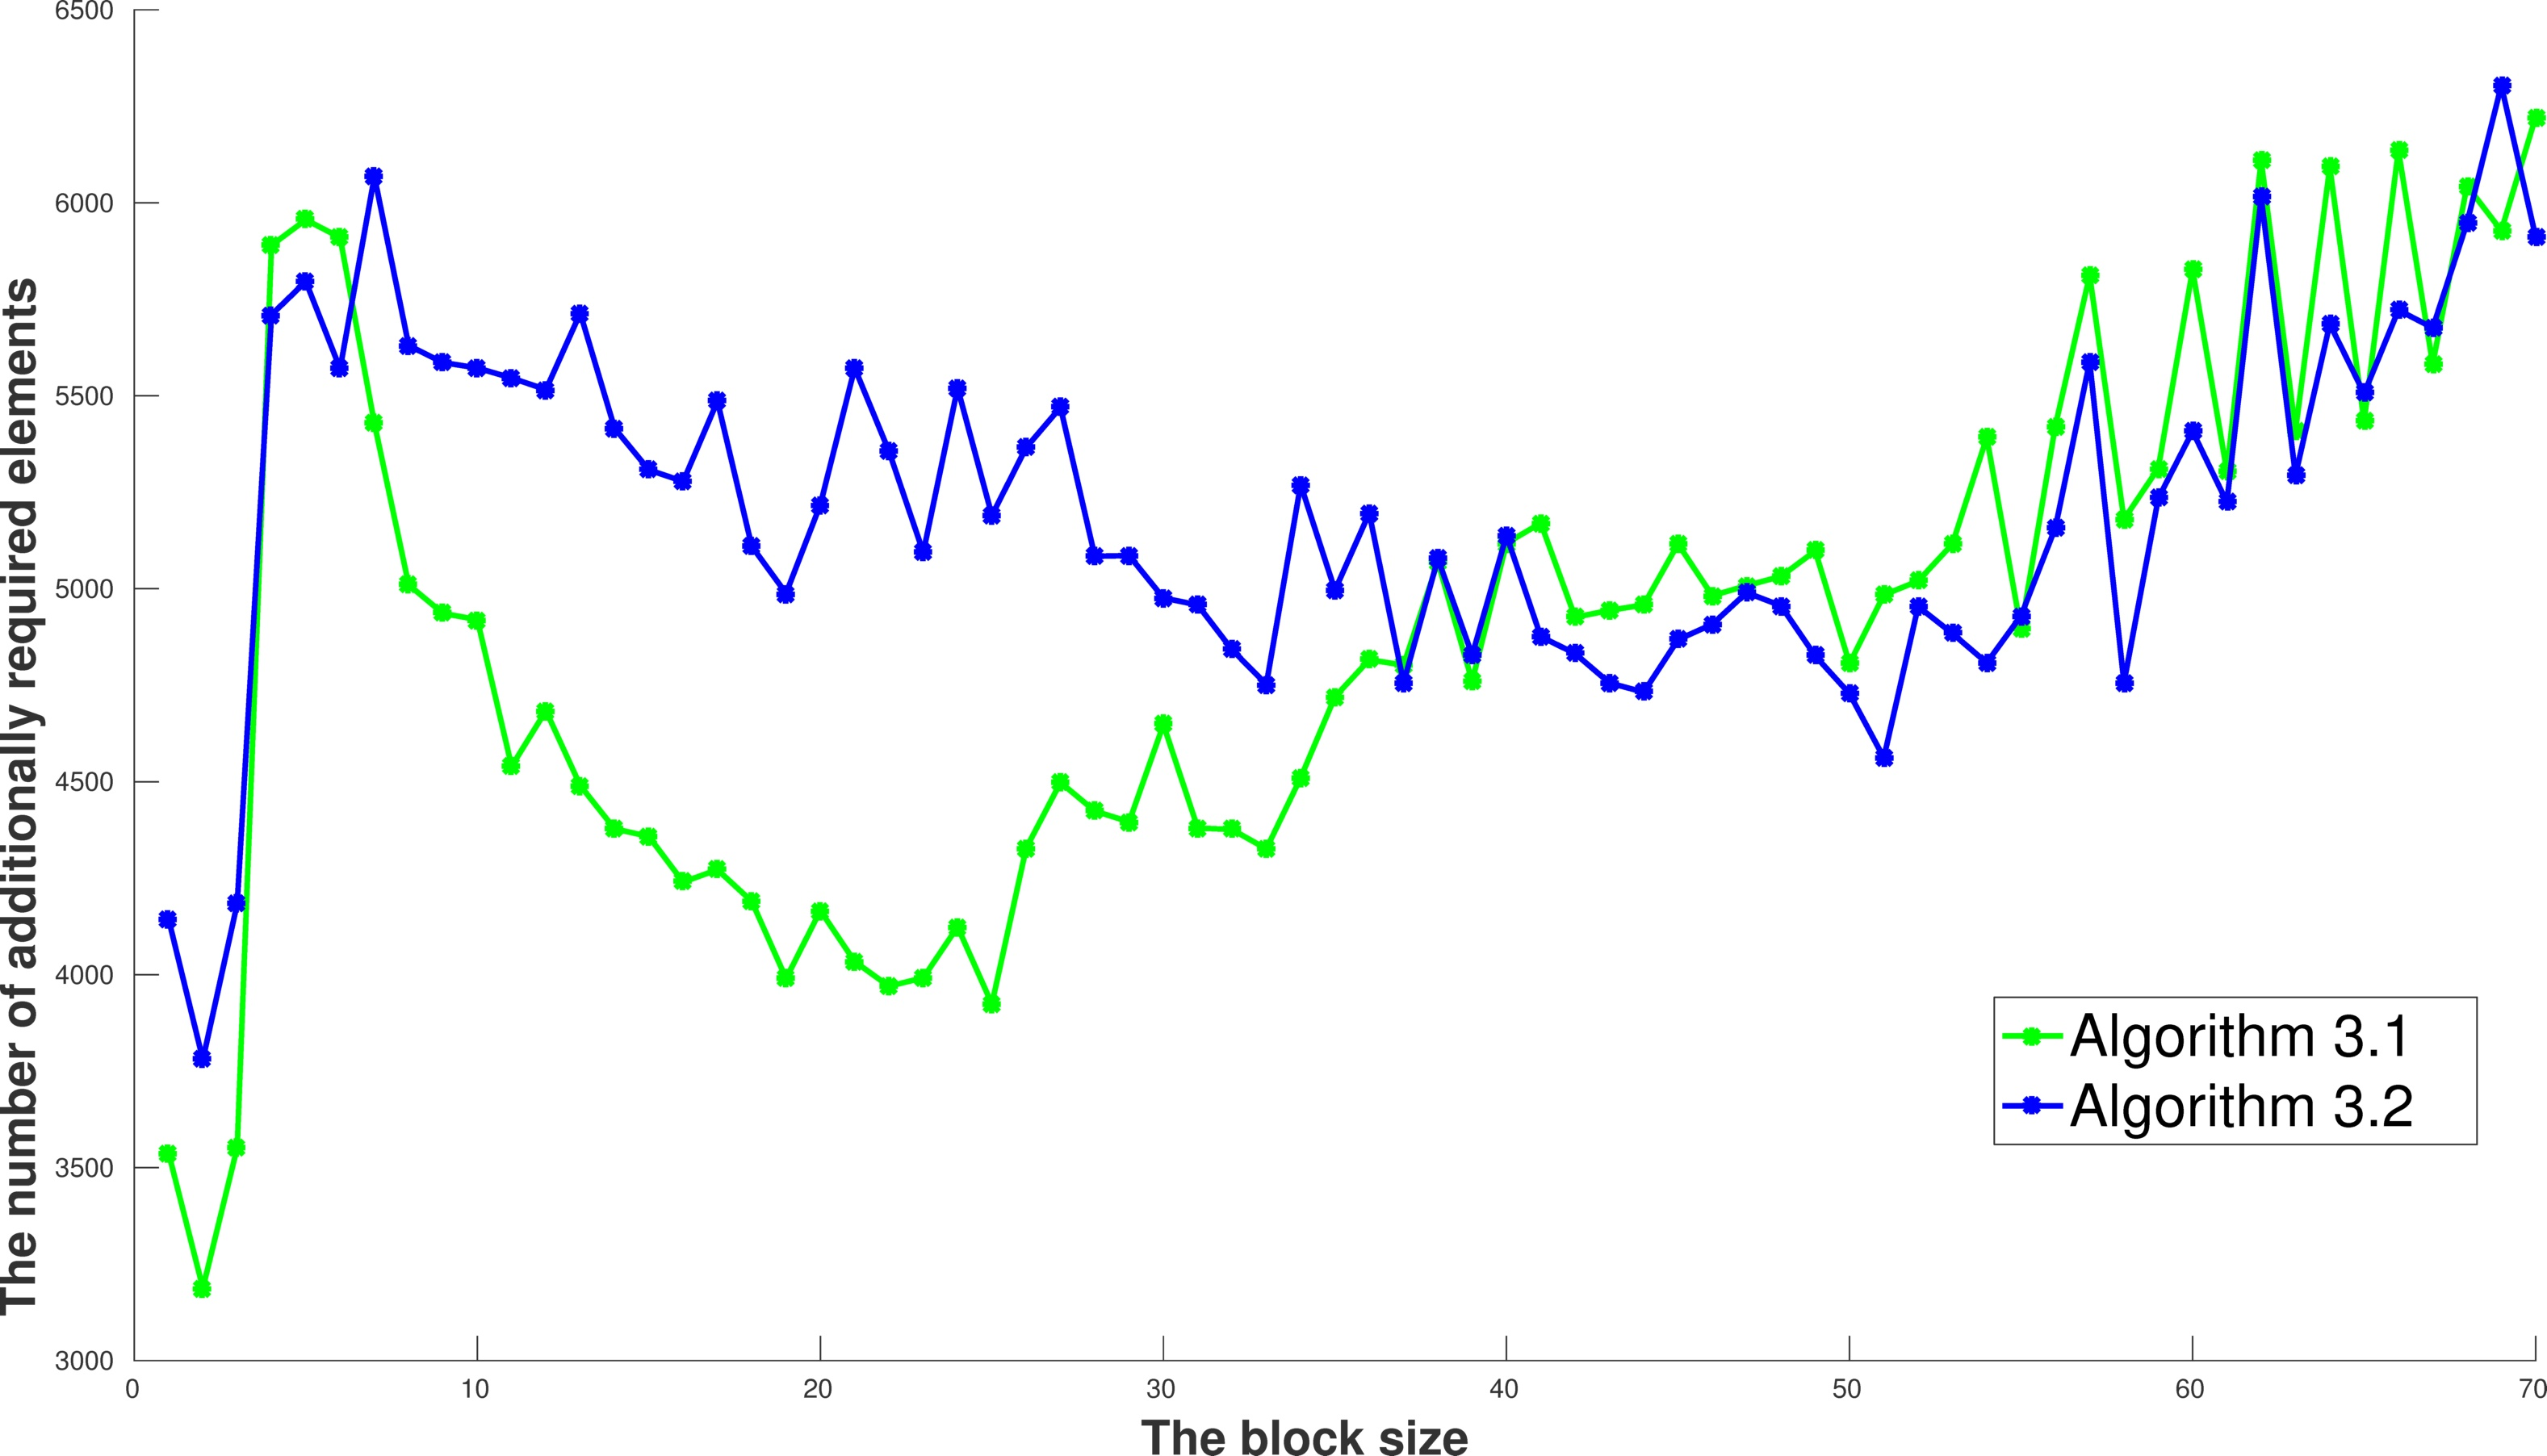
\includegraphics[width=0.9\linewidth]{ex33_alg31_alg32_bls_nat_add}
\caption{The number of additionally required elements computed by
\coderef{code.new.d2.nreq} with the natural ordering
compared with \coderef{code.greedy}.
The computation is carried out on the matrix \textit{ex33}. }
\label{ex33_alg31_alg32_bls_nat_add}
\end{figure}

\begin{figure}
\centering
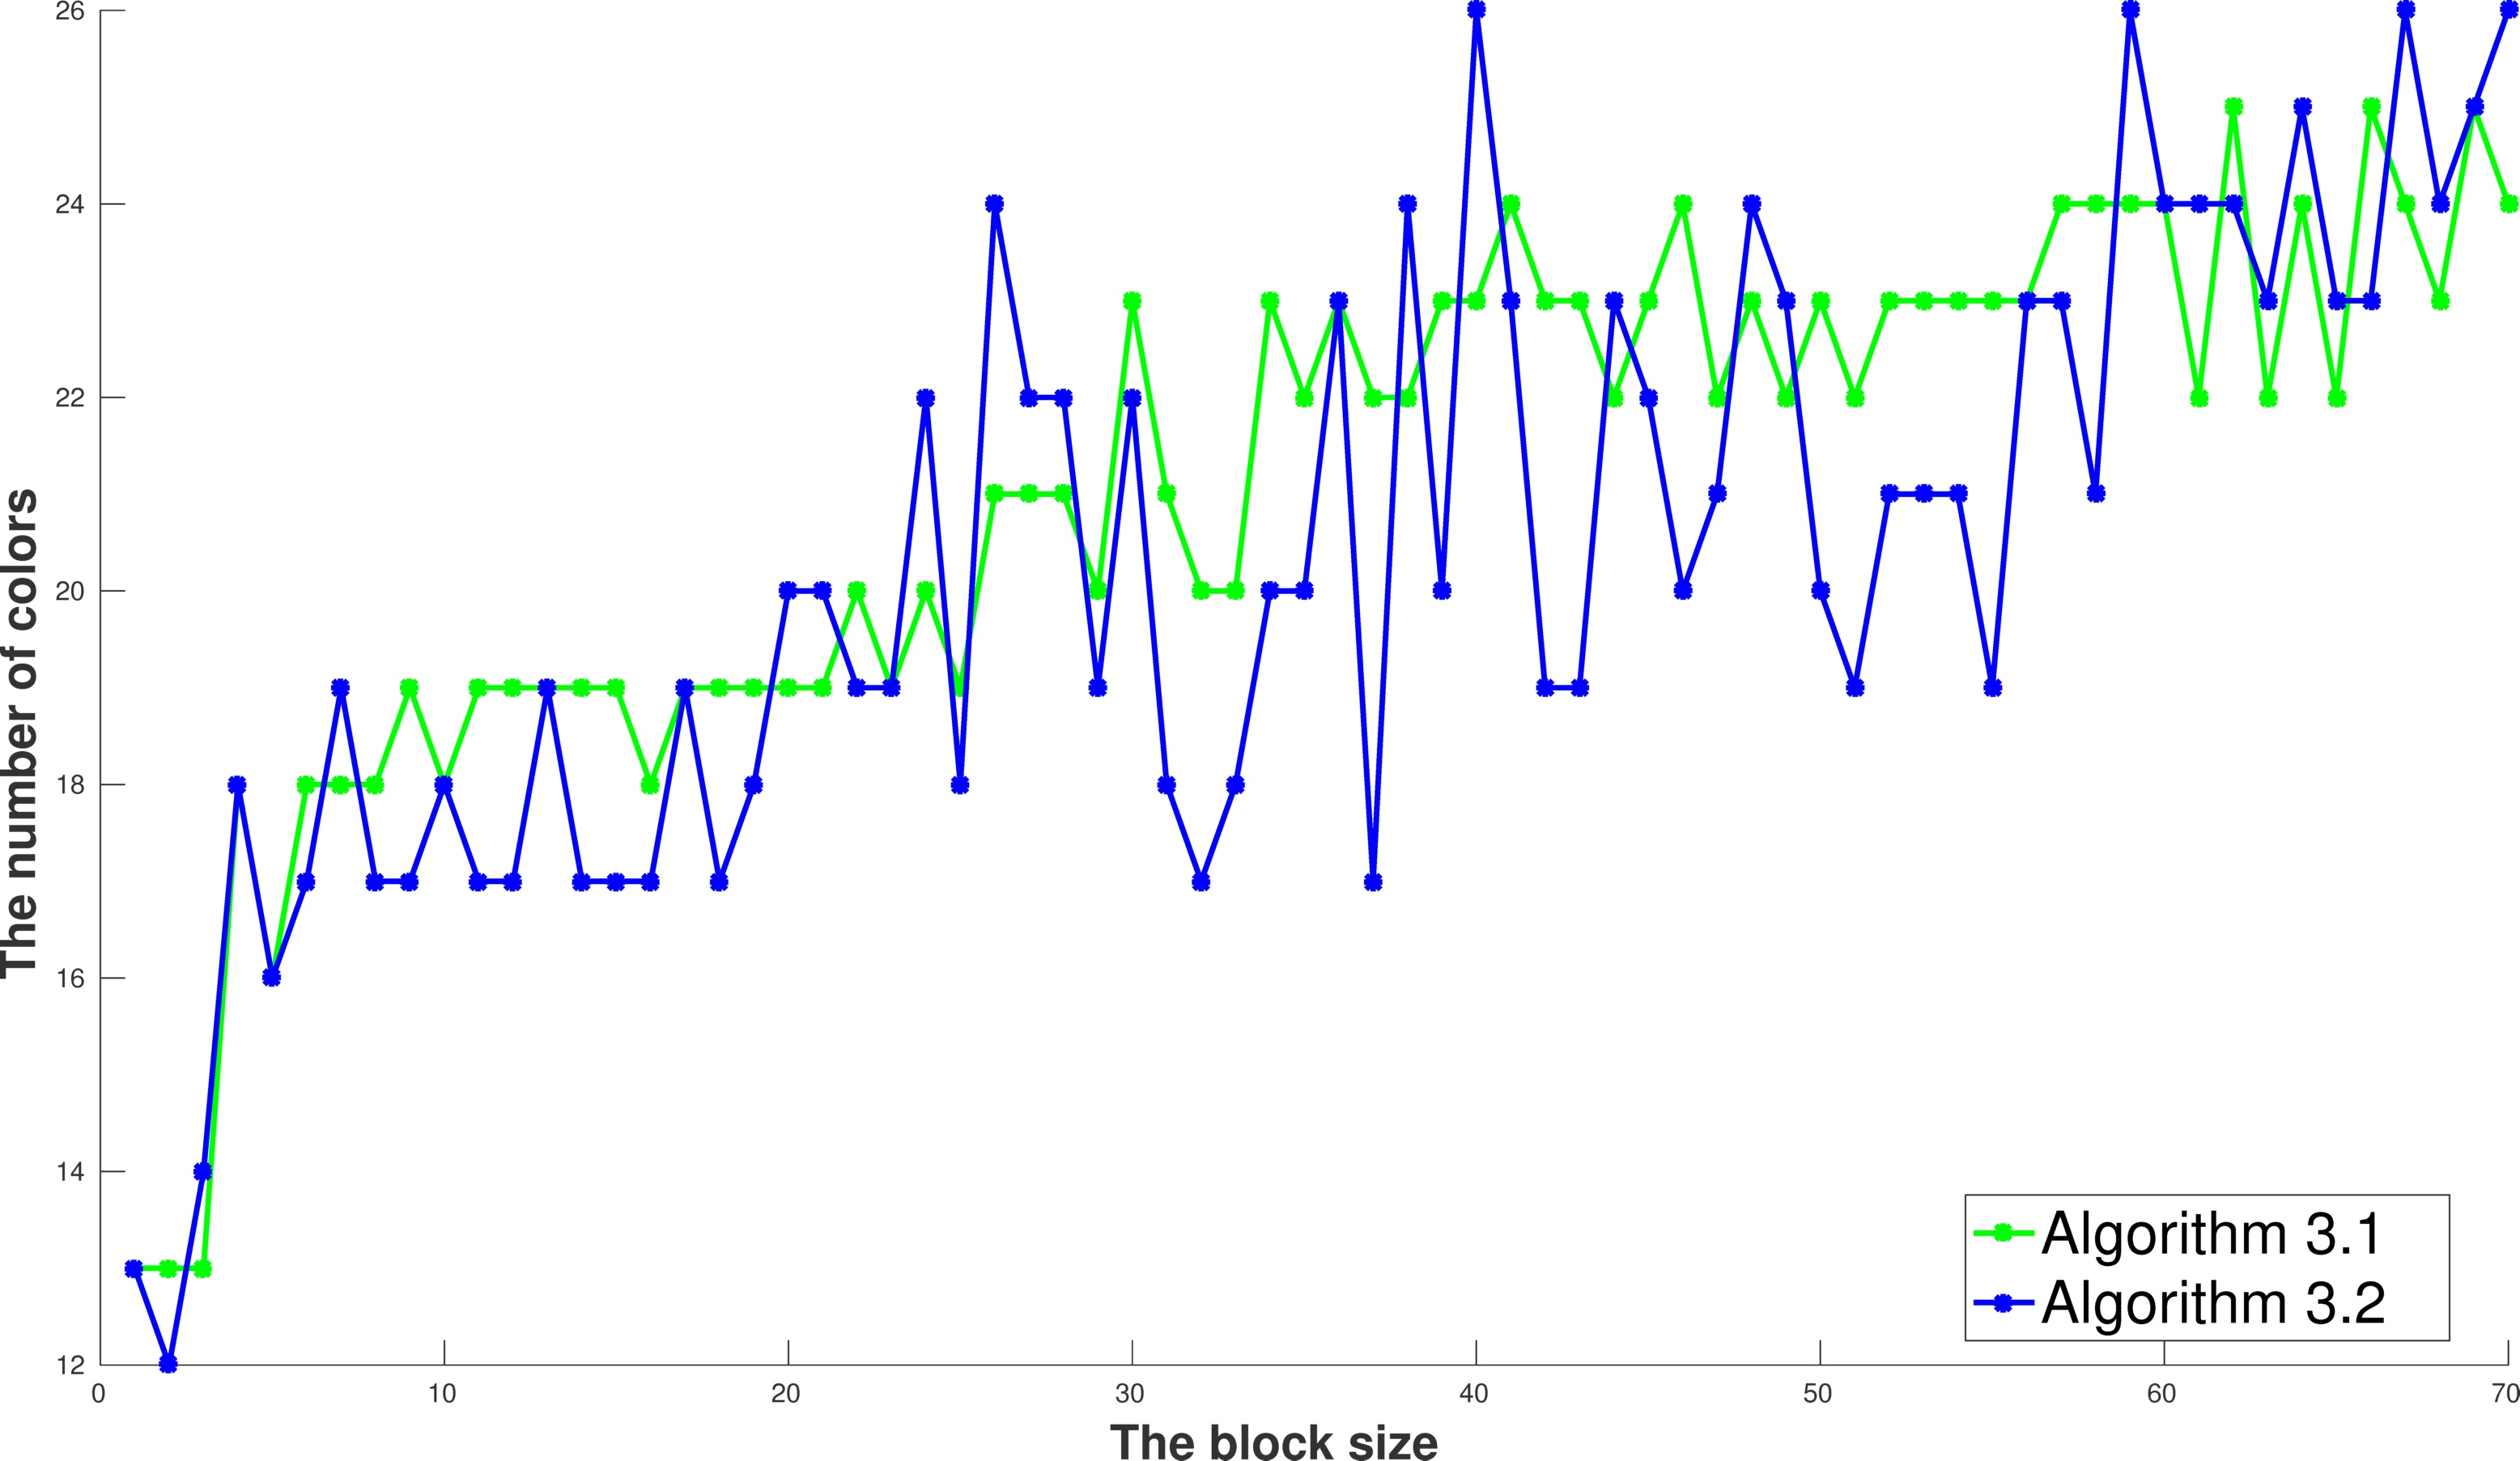
\includegraphics[width=0.9\linewidth]{ex33_alg31_alg32_bls_nat_cols}
\caption{The number of colors computed by \coderef{code.new.d2.nreq} with the natural ordering
compared with \coderef{code.greedy}.
The computation is carried out on the matrix \textit{ex33}. }
\label{ex33_alg31_alg32_bls_nat_cols}
\end{figure}

\begin{figure}
\begin{lstlisting}[
caption=A modification of \coderef{code.new.d2.nreq}.,
label=code.new.impr1,mathescape]
function d2_color_nreq_modified($G=(V_r\cup V_c,E)$,$E_i\subseteq E$)
  $\Phi\leftarrow [0\ldots 0]$
  $forbiddenColors\leftarrow [0\ldots 0]$
  for $v\in V_c$ with $\exists r\in V_r: (v,r) \in E_i$ and $\Phi(v)=0$
    for $n\in N_2(v,E_i)$ with $\Phi(n) \neq 0$
      $forbiddenColors[\Phi(n)] = v$
    $\Phi(v) = \min \{ a>0:forbiddenColors[a]\neq v\}$

    $I_v=\{z\in V_c: z\neq v\text{ and }z\notin N_2(v) \text{ and } \Phi(z) = 0 \}$
    if $I_v\neq\emptyset$
      $maxs = \argmax_{x\in I_v} \nreq_v (x)$
      $mins = \argmin_{x\in maxs} \req (x)$
      $\Phi(mins[0]) = \Phi(v)$
  return $\Phi$
\end{lstlisting}
\end{figure}

\begin{figure}
\centering
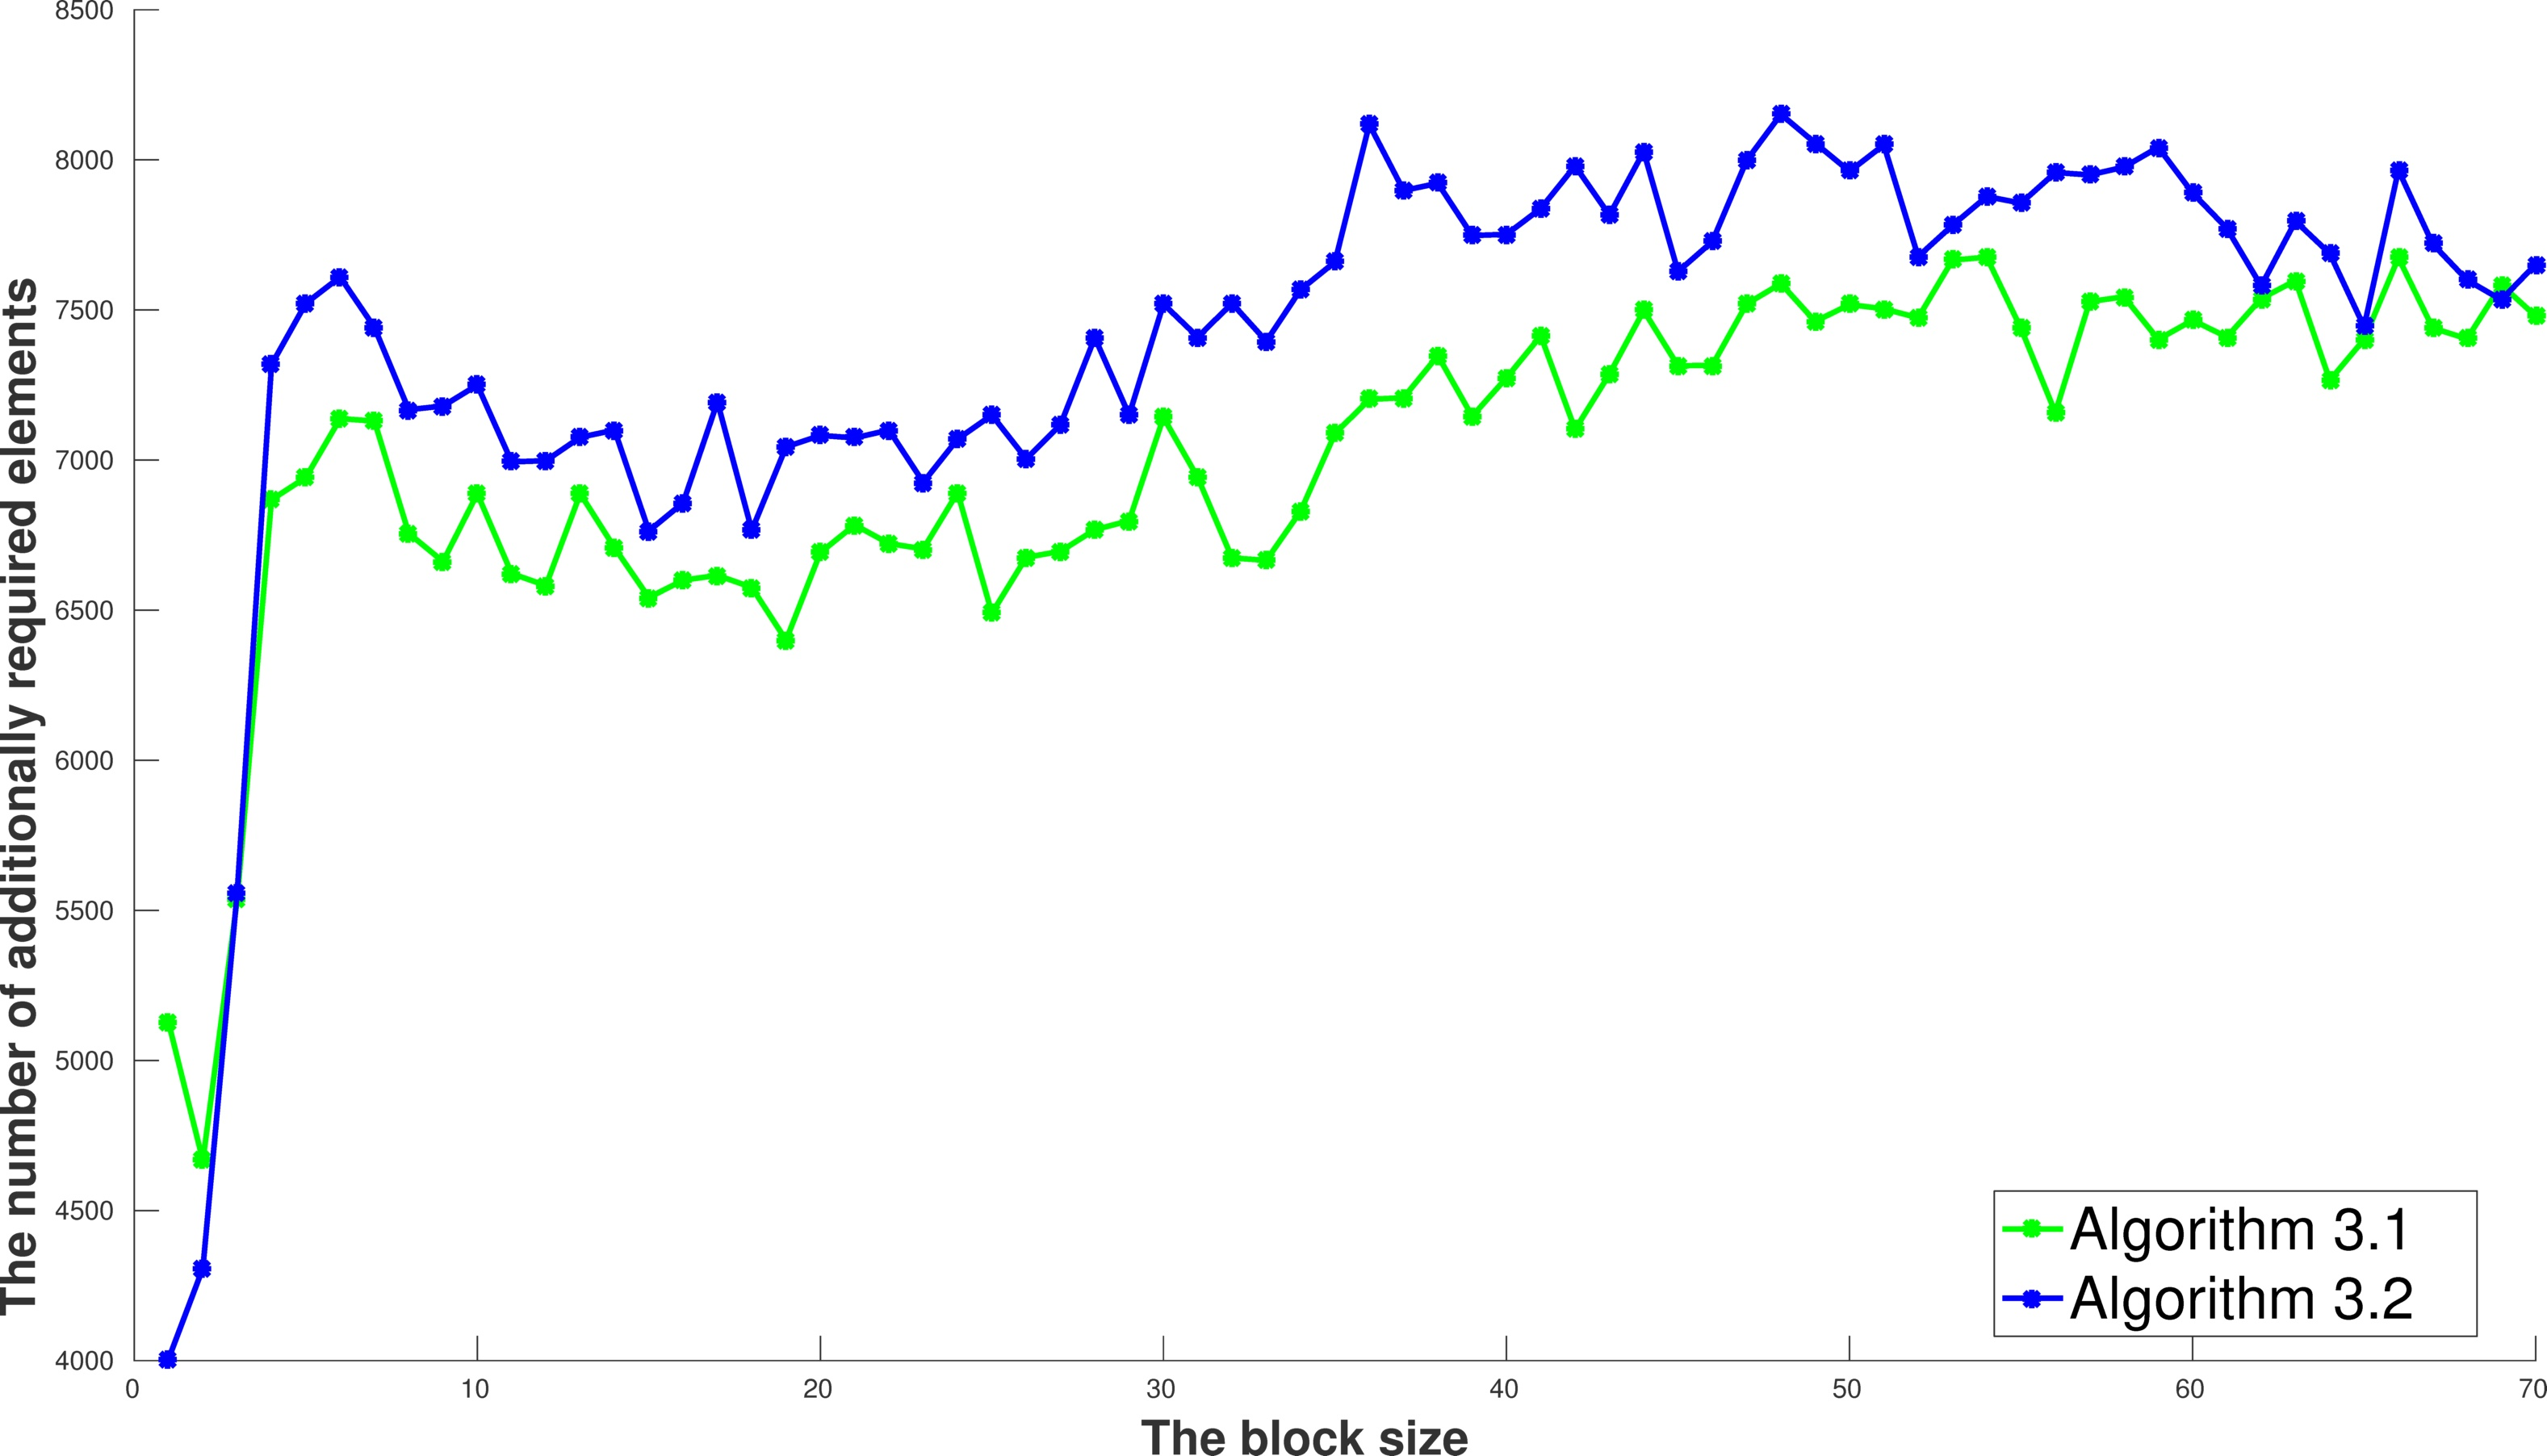
\includegraphics[width=0.9\linewidth]{ex33_alg32_alg34_bls_lfo_add}
\caption{The number of additionally
required elements is increased comparing \coderef{code.new.d2.nreq}
and \coderef{code.new.impr1} when the ordering for the coloring is the LFO ordering.
The computation is carried out on the matrix \textit{ex33}. }
\label{ex33_alg32_alg34_bls_lfo_add}
\end{figure}

Now, we modify \coderef{code.new.d2.nreq} further to select a vertex with the minimum number of
required elements among the computed set of vertices with the maximum number of determined nonrequired elements.
This idea facilitates gathering of more nonrequired elements in the same column since
more zero elements remain. These elements might offer more options for increasing the number of determined
nonrequired elements.
Let the function $\req: V_c\rightarrow \mathbb{N}$ compute the number of required edges adjacent to a vertex.
A new algorithm is proposed in \coderef{code.new.impr1} which applies this idea.
The only new difference of this algorithm to \coderef{code.new.d2.nreq}
is to compute the operator $\argmin$ for the
function $\req$. This computation has the same complexity as the computation of $\argmax$.
It means the time complexity is still as before.
\figref{ex33_alg32_alg34_bls_lfo_add} shows how the number of additionally
required elements is increased comparing
\coderef{code.new.d2.nreq} and \coderef{code.new.impr1} when the ordering for the coloring
is the LFO ordering. However, this is not the same for all matrices.
\appref{app.compare.alg32.alg34} shows the results for different matrices
and different orderings for the block size fixed to $10$.
Except the matrix \textit{ex7},
a general observation is that the numbers of additionally and potentially required elements
are decreased when the number of colors is decreased.
This brings us to the next topic of balancing the number of colors
and the number of additionally required elements.

\subsubsection{Balancing the number of colors}
Here, we modify \coderef{code.new.d2.nreq} and \coderef{code.new.impr1} again
to have a control over the balance between the number of
colors and the number of additionally required elements.
It means we define a balance variable $\alpha \in \mathbb{N}$ such that increasing this variable
would decrease both the number of colors and additionally required elements and vice versa.
\coderef{code.new.impr2} presents the new algorithm.
Rather than adding a single vertex as in \coderef{code.new.impr1},
the idea is to add more vertices representing columns
with the minimum number of required elements
and the maximum number of determined nonrequired elements.
This is implemented by coloring all elements of $mins$ with indices from $0$ to $\alpha-1$ .
%If the variable $\alpha=0$, we would have the same algorithm as \coderef{code.new.impr1}.
\begin{figure}
\begin{lstlisting}[
caption=New coloring heuristic with a controller to balance
the number of colors and the number of additionally required elements.,
label=code.new.impr2,mathescape]
function d2_color_nreq_balance($G=(V_r\cup V_c,E)$,$E_i\subseteq E$,$\alpha$)
  $\Phi\leftarrow [0\ldots 0]$
  $forbiddenColors\leftarrow [0\ldots 0]$
  for $v\in V_c$ with $\exists r\in V_r: (v,r) \in E_i$ and $\Phi(v)=0$
    for $n\in N_2(v,E_i)$ with $\Phi(n) \neq 0$
      $forbiddenColors[\Phi(n)] = v$
    $\Phi(v) = min \{ a>0:forbiddenColors[a]\neq v\}$

    $I_v=\{z\in V_c: z\neq v\text{ and }z\notin N_2(v) \text{ and } \Phi(z) = 0 \}$
    if $I_v\neq\emptyset$
      $maxs = \argmax_{x\in I_v} \nreq_v (x)$
      $mins = \argmin_{x\in maxs} \req(x)$
      for $i\in\{0,1,...,\min (\alpha - 1, size(mins)-1)\}$
        $\Phi(mins[i]) = \Phi(v)$
  return $\Phi$
\end{lstlisting}
\end{figure}

\figref{ex33_alg31_alg32_alg34_alg35_bls_lfo_cols}
shows the comparison between the number of colors computed by
the three presented algorithms: \coderef{code.new.d2.nreq},
\coderef{code.new.impr1}, and~\coderef{code.new.impr2}.
All these algorithms are computed with the LFO ordering.
We selected this ordering for this computation
since this ordering gives the best results.
The variable $\alpha$ for \coderef{code.new.impr2} is equal to $10$.
The block size varies also from $1$ to $70$.
It is clear from this figure that \coderef{code.new.impr2} tends to generate the
smallest number of colors particularly in the middle block sizes when $\alpha=10$.
However, as illustrated in \figref{ex33_alg31_alg32_alg34_alg35_bls_lfo_adds},
it does not perform well in the case of additionally required elements.

\begin{figure}
\centering
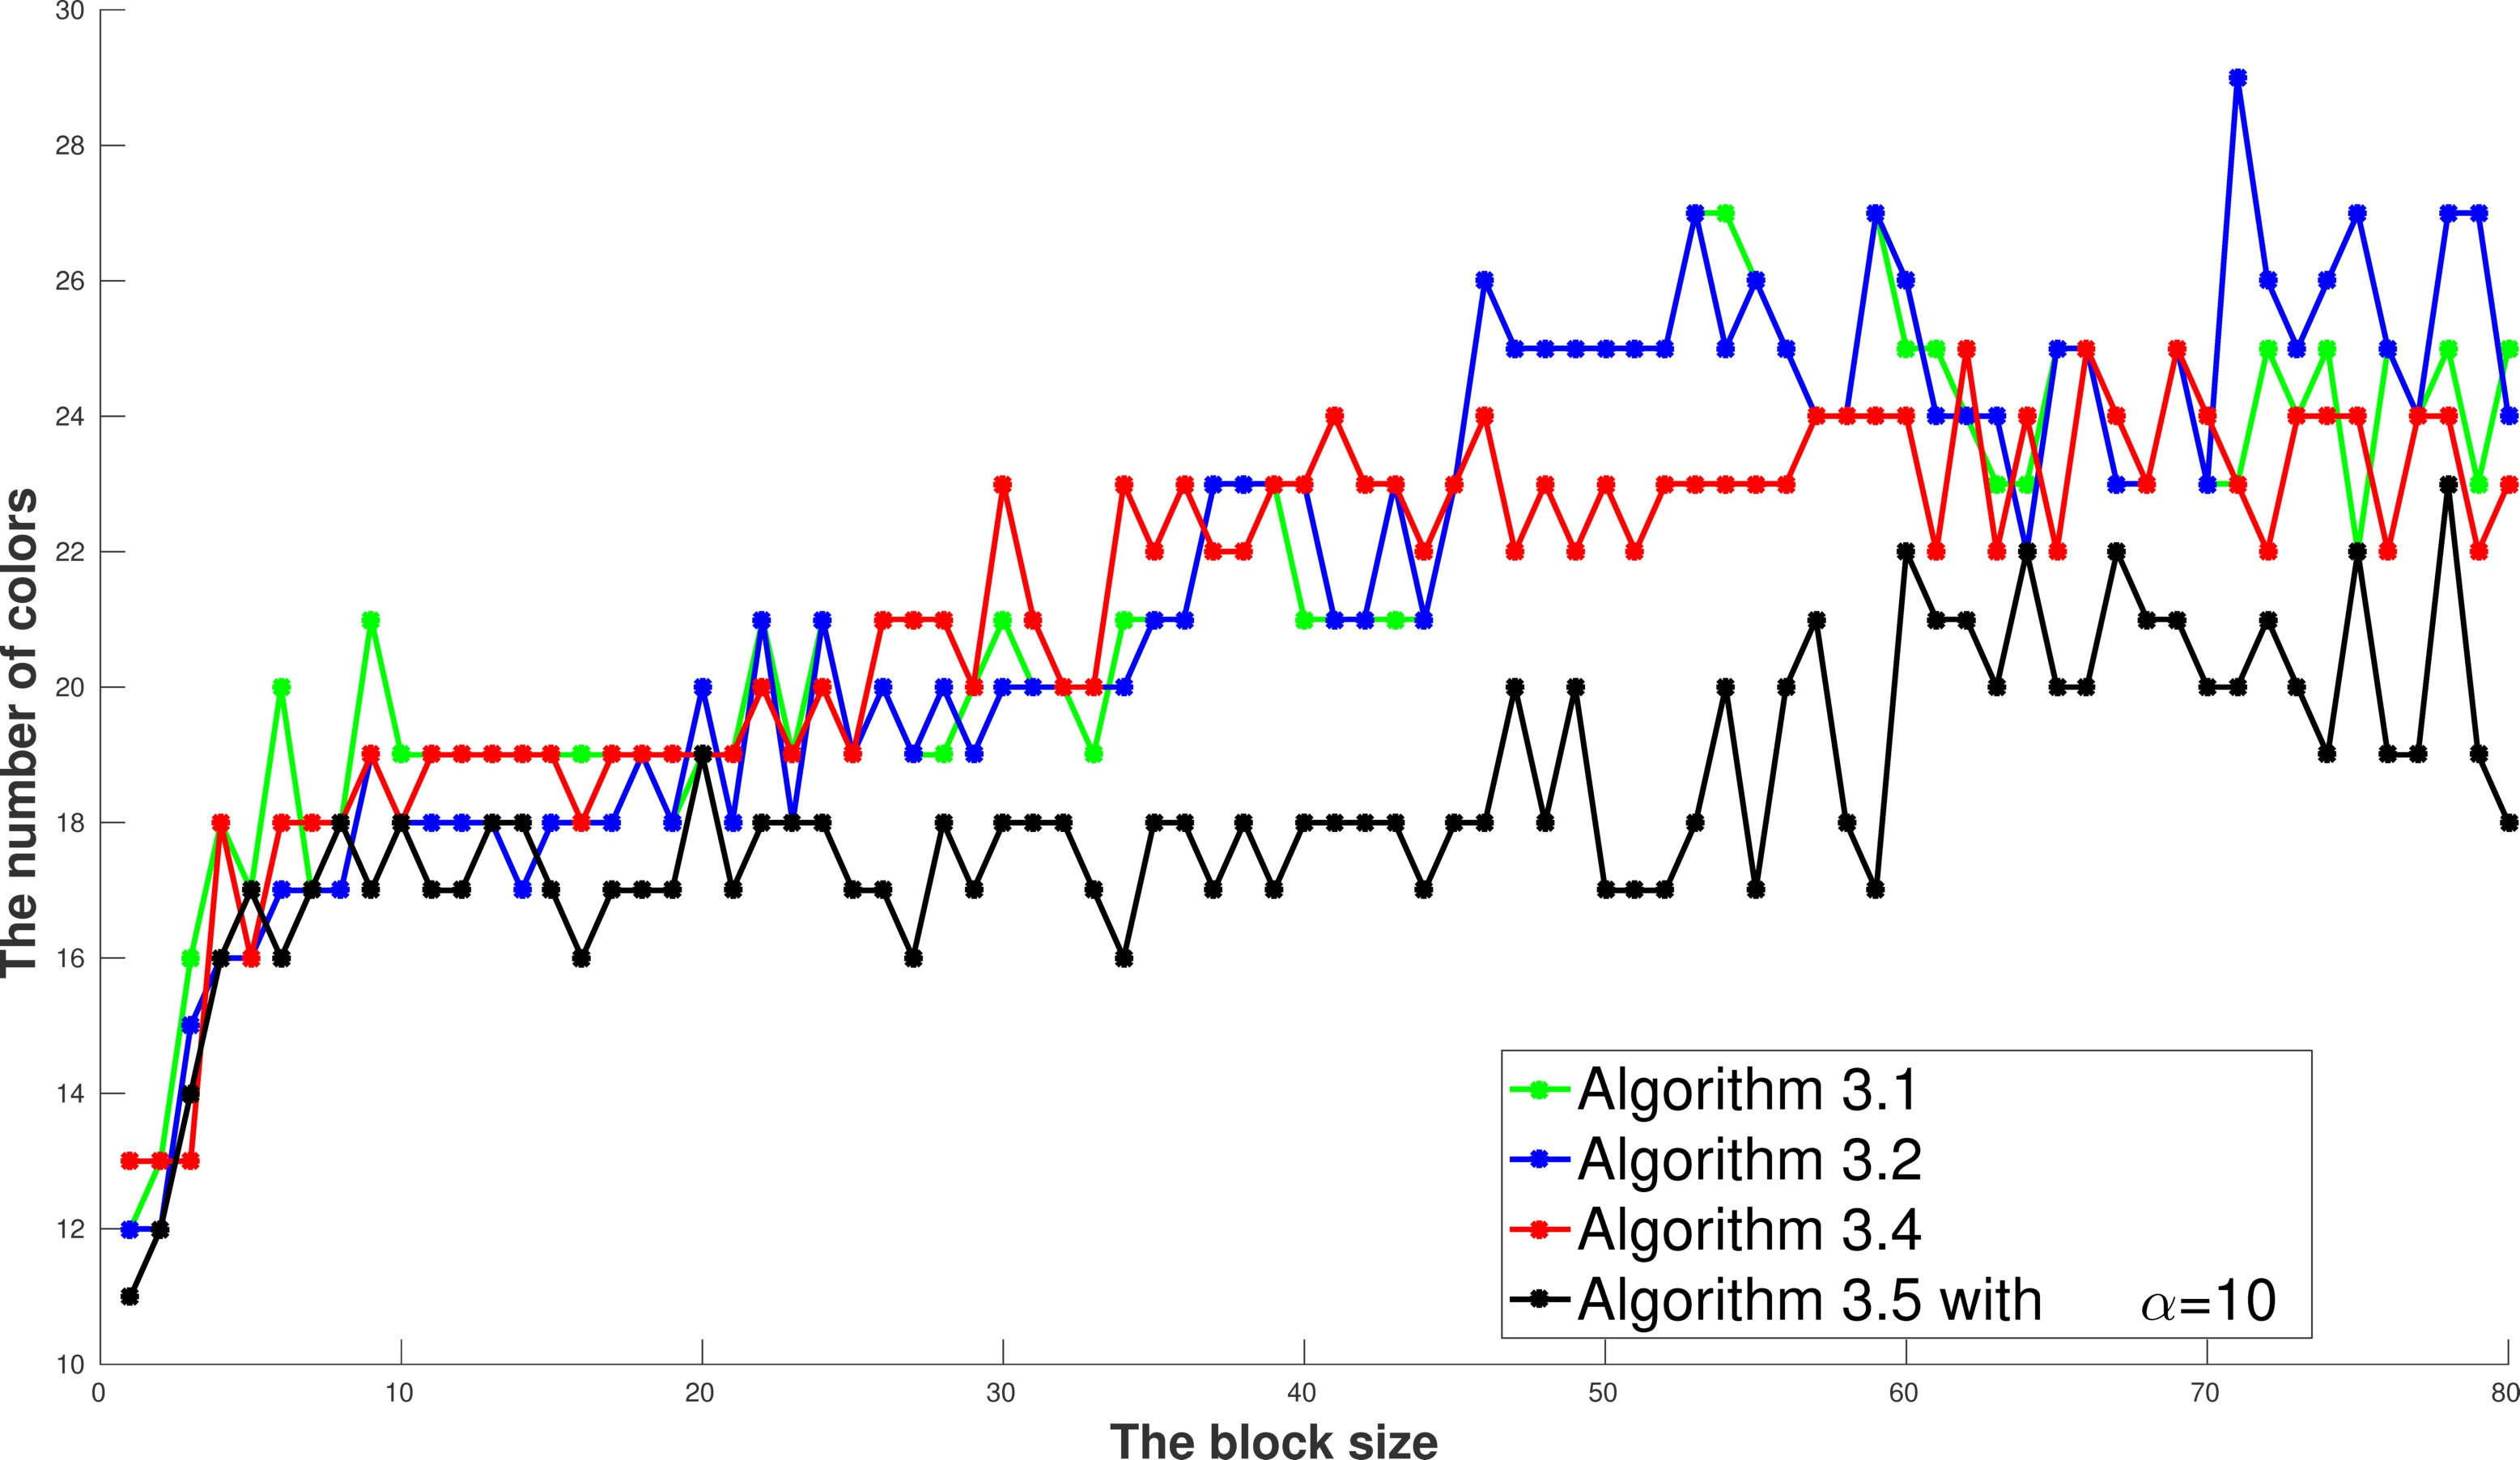
\includegraphics[width=0.9\linewidth]{ex33_alg31_alg32_alg34_alg35_bls_lfo_cols}
\caption{
The comparison of the number of colors in \coderef{code.new.d2.nreq},
\coderef{code.new.impr1}, and~\coderef{code.new.impr2}.
The computation is carried out on the matrix \textit{ex33} and with the LFO ordering.}
\label{ex33_alg31_alg32_alg34_alg35_bls_lfo_cols}
\end{figure}

\begin{figure}
\centering
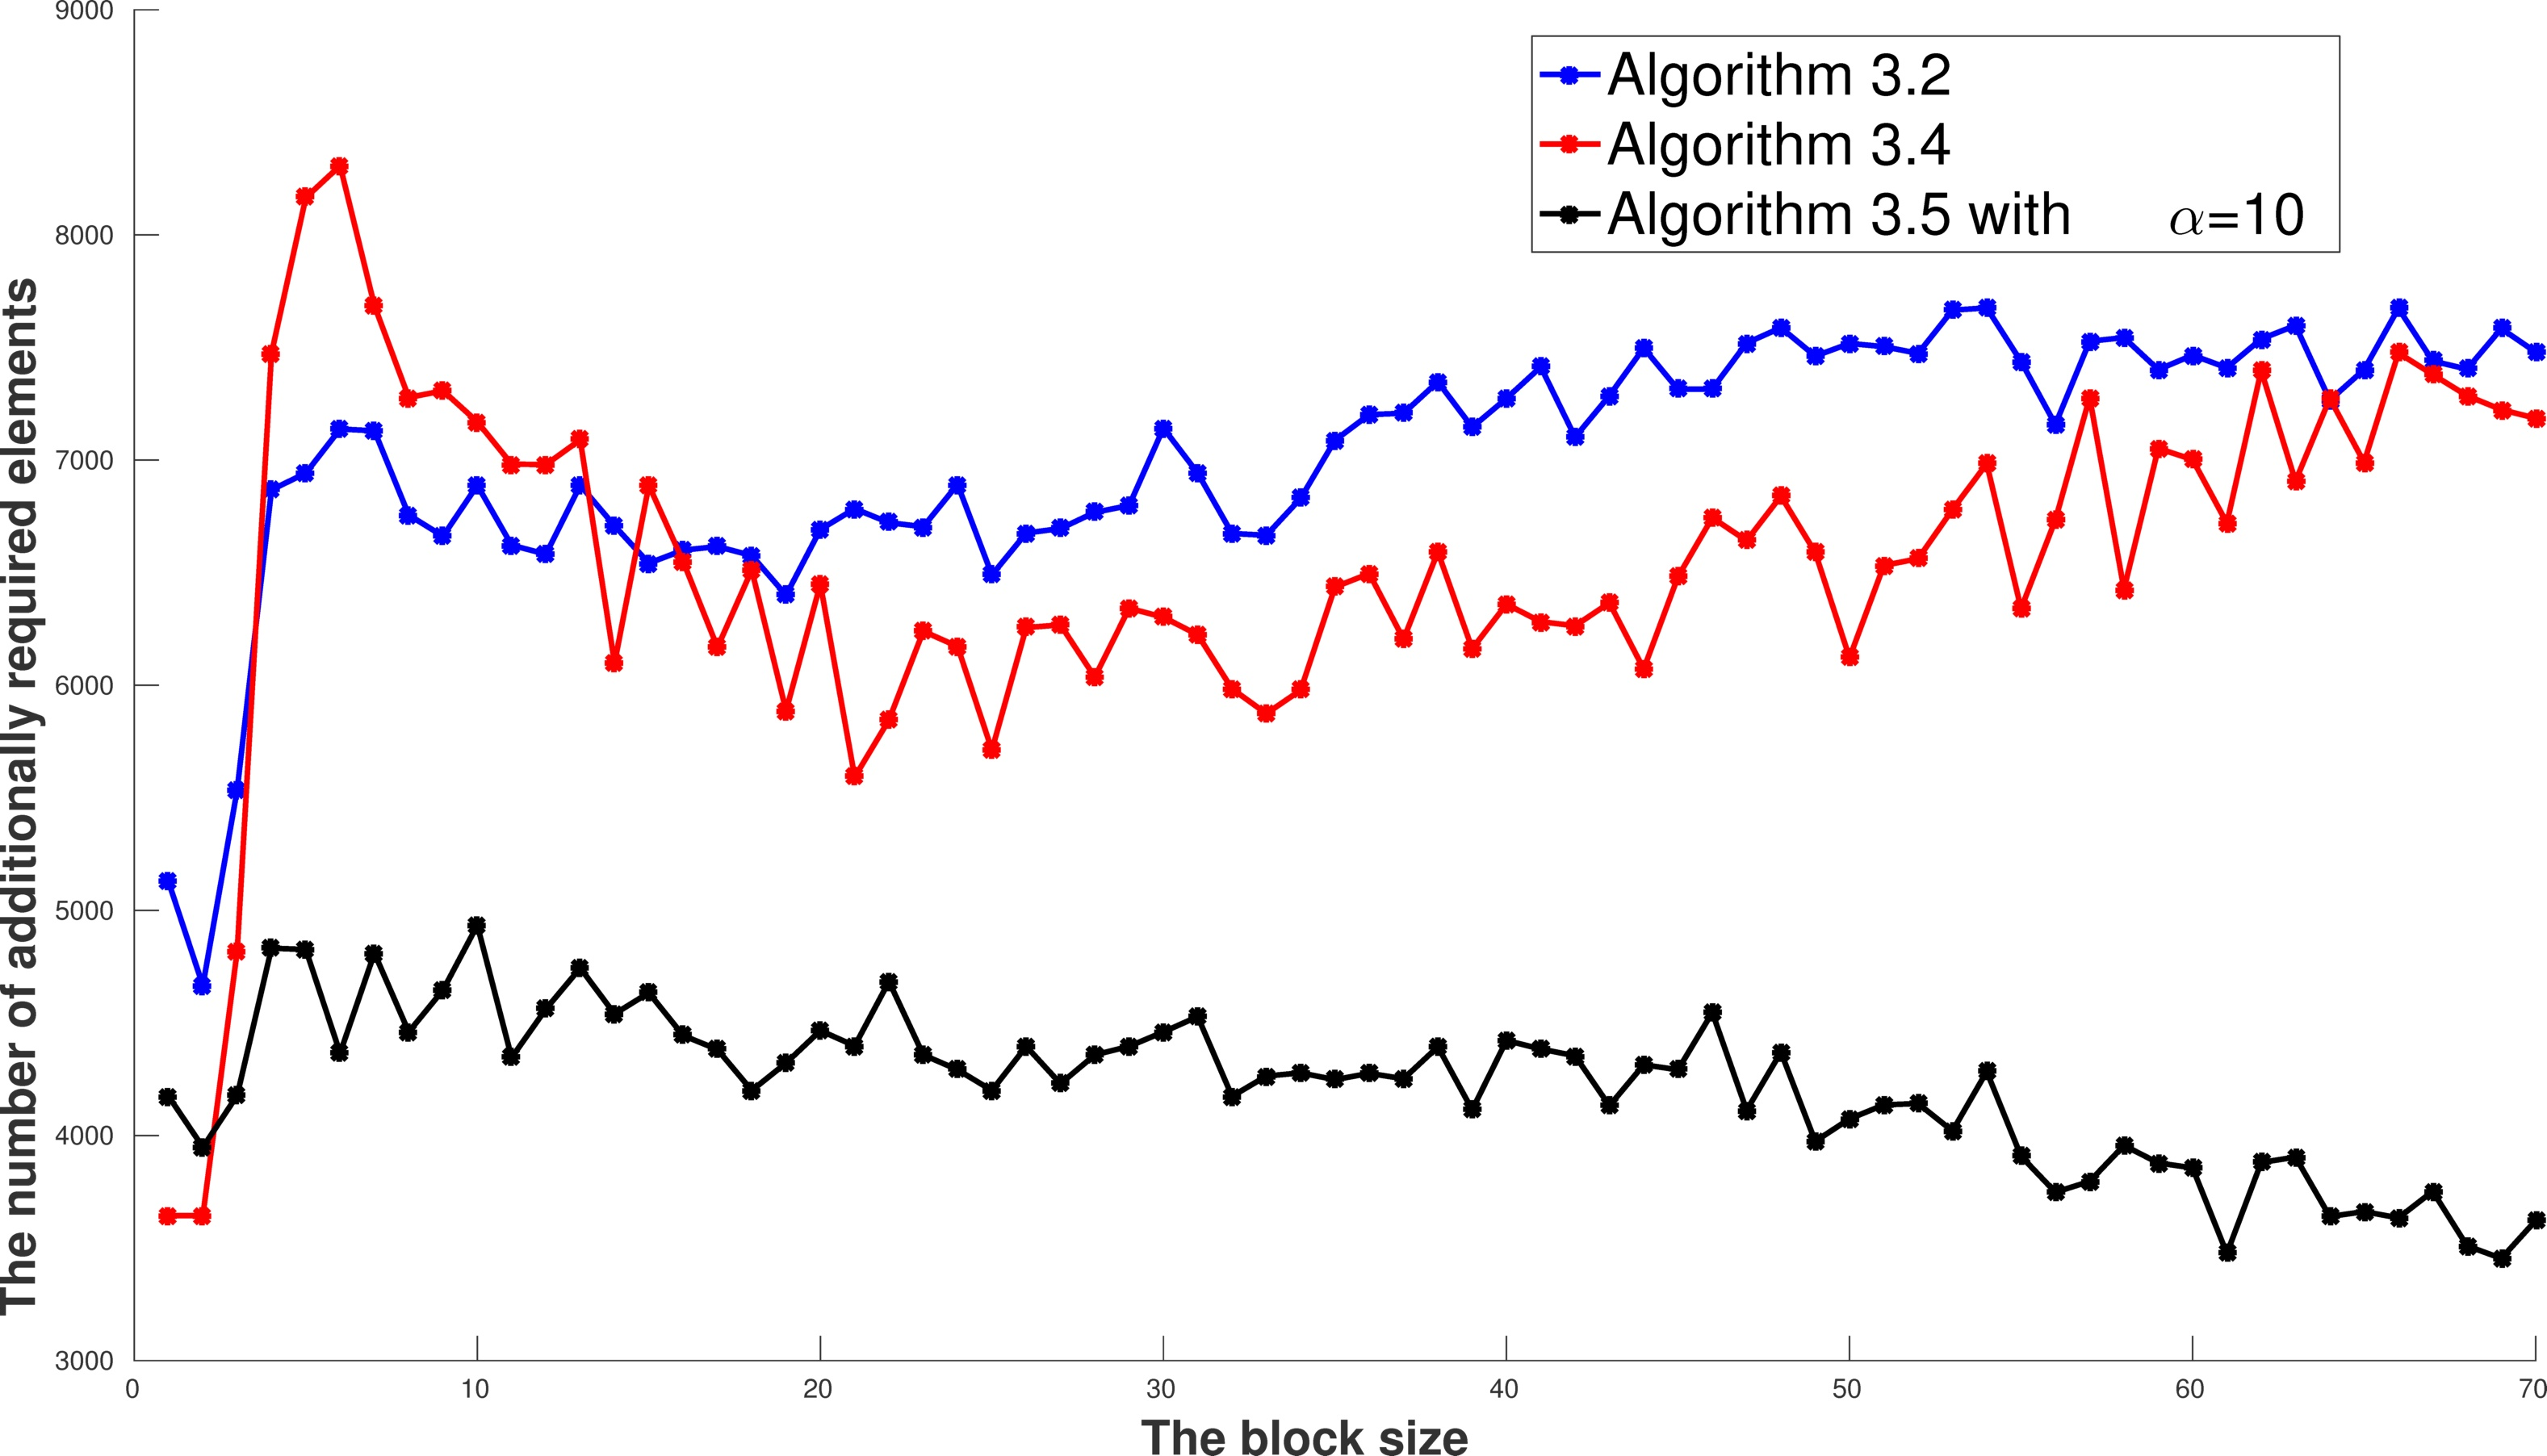
\includegraphics[width=0.9\linewidth]{ex33_alg31_alg32_alg34_alg35_bls_lfo_adds}
\caption{
The comparison of the number of additionally required elements in \coderef{code.new.d2.nreq},
\coderef{code.new.impr1}, and~\coderef{code.new.impr2}.
The computation is carried out on the matrix \textit{ex33} and with the LFO ordering.}
\label{ex33_alg31_alg32_alg34_alg35_bls_lfo_adds}
\end{figure}

Table~\ref{different.alpha} compares the number of additionally required elements and
the number of colors using \coderef{code.new.impr2} with different $\alpha$.
Three tables at the top, middle, and the bottom of Table~\ref{different.alpha}
are for the natural ordering, the LFO ordering, and the SLO ordering, respectively.
Regardless of the ordering and except for certain cases,
the number of colors tends to decrease when $\alpha$ grows.
Indeed, the number of colors is reduced in most of the cases. In some cases like
the matrix \textit{steam2.mtx} with the LFO ordering, we need $6$ fewer colors comparing
the coloring with $\alpha=0$ and $\alpha=10$.

On the other hand, except for certain cases,
the number of additionally required elements decreases
when $\alpha$ increases in the coloring.
However, in this table,
the coloring with $\alpha=6$ can be a suitable choice in most of the cases
since the number of additionally required elements is relatively high
while the number of colors is mainly small.
More figures can be found in \appref{app.compare.alg35.alphas} comparing these values
based on the varying block sizes.

\begin{table}
\centering
\begin{tabular}{|c|c|c|c|c|c|c|}
\hline
Matrix (NAT) & \multicolumn{6}{c|}{\coderef{code.new.impr2}} \\\hline
{} & \multicolumn{3}{c|}{$|R_{a}|$} & \multicolumn{3}{c|}{$|\Phi|$}\\\hline
{}     & $\alpha=0$ & $\alpha=6$ & $\alpha=10$ & $\alpha=0$& $\alpha=6$&$\alpha=10$ \\\hline
\textit{steam1.mtx} & $566$ & $440$ & $370$ & $10$ & $9$ & $8$ \\\hline
\textit{steam2.mtx} & $1512$ & $944$ & $1032$ & $13$ & $10$ & $9$ \\\hline
\textit{nos3.mtx} & $3416$ & $2778$ & $2348$ & $20$ & $18$ & $17$ \\\hline
\textit{ex7.mtx} & $23958$ & $22656$ & $21180$ & $55$ & $49$ & $46$ \\\hline
\textit{ex33.mtx} & $5992$ & $5616$ & $5262$ & $19$ & $18$ & $18$ \\\hline
\textit{crystm01.mtx} & $28348$ & $28466$ & $28516$ & $22$ & $24$ & $24$ \\\hline
\textit{coater1.mtx} & $7896$ & $7562$ & $7538$ & $30$ & $26$ & $25$ \\\hline
\end{tabular}
\vspace*{1cm}\newline
\begin{tabular}{|c|c|c|c|c|c|c|}
\hline
Matrix (LFO) & \multicolumn{6}{c|}{\coderef{code.new.impr2}} \\\hline
{} & \multicolumn{3}{c|}{$|R_{a}|$} & \multicolumn{3}{c|}{$|\Phi|$}\\\hline
{} & $\alpha=0$ & $\alpha=6$ & $\alpha=10$ & $\alpha=0$& $\alpha=6$&$\alpha=10$ \\\hline
\textit{steam1.mtx} & $518$ & $456$ & $330$ & $12$ & $10$ & $10$ \\\hline
\textit{steam2.mtx} & $1280$ & $660$ & $564$ & $17$ & $13$ & $11$ \\\hline
\textit{nos3.mtx} & $3646$ & $2360$ & $2190$ & $20$ & $19$ & $19$ \\\hline
\textit{ex7.mtx} & $22532$ & $21444$ & $21576$ & $49$ & $48$ & $47$ \\\hline
\textit{ex33.mtx} & $5968$ & $5222$ & $4934$ & $16$ & $17$ & $16$ \\\hline
\textit{crystm01.mtx} & $21168$ & $21918$ & $21210$ & $18$ & $18$ & $18$ \\\hline
\textit{coater1.mtx} & $7210$ & $7168$ & $6998$ & $23$ & $23$ & $23$ \\\hline
\end{tabular}
\vspace*{1cm}\newline
\begin{tabular}{|c|c|c|c|c|c|c|}
\hline
Matrix (SLO) & \multicolumn{6}{c|}{\coderef{code.new.impr2}} \\\hline
{} & \multicolumn{3}{c|}{$|R_{a}|$} & \multicolumn{3}{c|}{$|\Phi|$}\\\hline
{} & $\alpha=0$ & $\alpha=6$ & $\alpha=10$ & $\alpha=0$& $\alpha=6$&$\alpha=10$ \\\hline
\textit{steam1.mtx} & $748$ & $476$ & $390$ & $14$ & $13$ & $13$ \\\hline
\textit{steam2.mtx} & $1816$ & $1024$ & $980$ & $17$ & $12$ & $11$ \\\hline
\textit{nos3.mtx} & $3998$ & $2620$ & $1978$ & $20$ & $18$ & $17$ \\\hline
\textit{ex7.mtx} & $23598$ & $22362$ & $22098$ & $52$ & $50$ & $49$ \\\hline
\textit{ex33.mtx} & $6174$ & $5752$ & $4902$ & $19$ & $18$ & $17$ \\\hline
\textit{crystm01.mtx} & $27432$ & $26478$ & $27782$ & $22$ & $22$ & $22$ \\\hline
\textit{coater1.mtx} & $7668$ & $7624$ & $7570$ & $25$ & $26$ & $24$ \\\hline
\end{tabular}
\caption{The comparison of the additionally required elements and the number of colors
in the computation of \coderef{code.new.impr2} with the different value of $\alpha$.
The orderings for coloring are (Top) the natural ordering,
(Middle) LFO, and (Bottom) SLO.}
\label{different.alpha}
\end{table}

%%%%%%%%%%%%%%%%%%%%%%%%%%%%%%%%%%%%%%%%%%%%%%%%%%%%%%%%%%%%%%%%%%%%%%%%%%%%
\clearpage
\subsubsection{Parallelization}
\label{s.parallel}
%%%%%%%%%%%%%%%%%%%%%%%%%%%%%%%%%%%%%%%%%%%%%%%%%%%%%%%%%%%%%%%%%%%%%%%%%%%%
For a faster computation, we parallelize the proposed heuristics by OpenMP.
There is much literature to parallelize coloring algorithms.
For example, {\c{C}}ataly{\"{u}}rek~\cite{cataly2012} introduced an OpenMP parallelized
greedy coloring which computes the same number of colors as the serial version.
However, there are two points in each iteration of the algorithm in which the threads
need to be synchronized.
Here, our focus is on another algorithm from Rokos et al.~\cite{Rokos2015}
which presents an algorithm in which only a single point of synchronization is needed.
In this algorithm, the number of colors changes with the number of parallel threads
but it remains near to the number of colors in the serial version.
We adapt this parallelization to \coderef{code.greedy} and \coderef{code.new.impr2} for the bipartite graph model.
These algorithms first color the vertices
greedily with a parallel loop and then correct the false coloring which can happen.

We color the bipartite graph associated with the matrix \textit{Cavity16}
from the sparse matrix collection of the university of Florida.
The timing results are all from the computations carried on an Intel Core i5 with 8 GB RAM with hyperthreading.
This means that the number of available parallel threads is doubled by hyperthreading resulting in $4$ threads.
Table~\ref{omp.res} shows the results of these computations.
Here, we change the number of threads from $1$ to $5$ shown in the first column.
The second column shows the computation time in milliseconds. The third column
is also the number of colors which changes based on the number of threads.
Here, the time decreases by increasing the number of threads up to $4$.
Then it decreases as we have only $4$ available threads.
Also, the number of colors changes slightly by increasing the number of threads.

\begin{figure}
\begin{tabular}{|c|c|c|}
\hline
Threads & Time & Colors \\\hline
1 & 42.8745 & 47 \\\hline
2 & 33.9665 & 47 \\\hline
3 & 25.2741 & 48 \\\hline
4 & 20.6863 & 48 \\\hline
5 & 21.4943 & 47 \\\hline
\end{tabular}\hfill
\begin{tabular}{|c|c|c|}
\hline
Threads & Time & Colors \\\hline
1 & 96.795 & 48 \\\hline
2 & 75.744 & 47 \\\hline
3 & 55.605 & 49 \\\hline
4 & 49.335 & 49 \\\hline
5 & 49.360 & 47 \\\hline
\end{tabular}
\caption{
(Left) The results of computation of OpenMP-parallelized \coderef{code.greedy}.
(Right) The results of computation of OpenMP-parallelized \coderef{code.new.impr2}.
}
\label{omp.res}
\end{figure}


%%%%%%%%%%%%%%%%%%%%%%%%%%%%%%%%%%%%%%%%%%%%%%%%%%%%%%%%%%%%%%%%%%%%%%%%%%%%%%%%%%%%%%%%%
\clearpage
\subsection{Restricted star bicoloring}
\label{s.heuristic.starbicoloring}
%%%%%%%%%%%%%%%%%%%%%%%%%%%%%%%%%%%%%%%%%%%%%%%%%%%%%%%%%%%%%%%%%%%%%%%%%%%%%%%%%%%%%%%%%%
Here, we search for a modified version of star bicoloring
which increases the number of potentially and additionally required elements without
a high increase in the number of colors.
We can apply the ideas from \coderef{code.new.impr1} and \coderef{code.new.impr2}.
However, we should not expect to have a high increase in the number of additionally required elements
that is equal to the sum of the increases in the column compression and row compression.

In \cite{Gebremedhin05whatcolor}, there is an algorithm called \textit{star bicoloring scheme}.
Lülfesmann~\cite{LulfesmannMaster} implemented and evaluated this algorithm.
This algorithm closely follows the definition of the star bicoloring.
Complete direct cover bicoloring~\cite{hs:csj}
is another algorithm which is introduced for bicoloring.
According to Calotoiu~\cite{CalotoiuMaster}, this algorithm does not perform
better than the star bicoloring scheme.
Also, Calotoiu~\cite{CalotoiuMaster} introduces two other algorithms the integrated star bicoloring
and total ordering star bicoloring which perform better than
the star bicoloring scheme for certain matrices and not much worse for other matrices.

We consider the implementation of star bicoloring in \coderef{orig.star.bicoloring} based on
the algorithm from Lülfesmann~\cite{Lulfesmann2012Fap}.
Here, the notation $G[S]$ means a graph $G$ induced by the edge set $S$.
Also, the notation $\Delta(V,G)$ represents the maximum degree of the vertices from $V$ in the graph $G$.
In this algorithm, the function \textit{next\_vertex} selects first which vertex should be processed in the next step.
Should it be from the column vertices or the row vertices?
This selection is based on the value of a weightening factor $\rho$ (to be explained below)
and a vertex with the maximum degree in each step.
After this selection, the conditions of the star bicoloring are analyzed in the next lines of this algorithm.
Two final loops of the algorithm are just post processing steps. The first one makes the colors distinct for the column and
row vertices. And the second one colors the uncolored vertices with the color $0$.
\begin{figure}
\begin{lstlisting}[
caption=Algorithm 3.5 from Lülfesmann~\cite{Lulfesmann2012Fap} for star bicoloring.,label=orig.star.bicoloring,mathescape]
function star_bicoloring($G=(V_r\cup V_c,E)$,$E_i\subseteq E$,$\rho$,next_vertex)
  $\Phi\leftarrow [-1\ldots -1]$
  $forbiddenColors\leftarrow [0\ldots 0]$
  $E_i^{'} = E_i$

  while $E_i^{'}\neq\emptyset$
    $v$=next_vertex($G$,$E_i^{'}$,$\rho$)
    $E_i^{'} = E_i^{'} - \{(v,w)\in E_i^{'}:w\in N_1(v,G[E_i^{'}])\}$
    for $w\in N_1(v,G)$
      if $\Phi(w) \leq 0$
        for $x\in N_1(w,G)$ with $\Phi(x) > 0$
          if $(v,w) \in E_i$ or $(w,x) \in E_i$
            $forbiddenColors[\Phi (x)]=v$
      else
        for $x\in N_1(w,G[E_i])$ with $\Phi(x) > 0$
        for $y\in N_1(x,G)$ with $\Phi(y) > 0$ and $y\neq w$
          if $\Phi(w) = \Phi(y)$
            $forbiddenColors[\Phi (x)] = v$

    $\Phi(v) = \min(\{j>0: forbiddenColors[j] \neq v\})$
  for $v_c\in V_c$ with $\Phi(v_c) > 0$
    $\Phi (v_c) = \Phi (v_c) + \max(\{\Phi (v_r): v_r \in V_r\})$
  for $v\in V_r\cup V_c$ with $\Phi(v)= -1$
    $\Phi (v) = 0$

  return $\Phi$

function next_vertex($G=(V_r\cup V_c,E)$,$E_i^{'}$,$\rho$)
  if($\Delta(V_r,G[E_i^{'}]) > \rho \Delta(V_c,G[E_i^{'}])$
    $v$ = $v_r\in V_r$ with maximum degree in $G[E_i^{'}]$
  else
    $v$ = $v_c\in V_c$ with maximum degree in $G[E_i^{'}]$
  return $v$
\end{lstlisting}

\begin{lstlisting}[
caption= Our new heuristic for star bicoloring considering the determined nonrequired elements.,
label=new.star.bicoloring,mathescape]
function star_bicoloring_nreq($G=(V_r\cup V_c,E)$,$E_i\subseteq E$,$\rho$)
  NonReq = false
  star_bicoloring($G$,$E_i$,$\rho$,next_vertex_nreq)

function next_vertex_nreq($G=(V_r\cup V_c,E)$,$E_i^{'}$,$\rho$)
  $v$ = next_vertex($G$,$E_i^{'}$,$\rho$)
  if NonReq = false
    NonReq = true
  else
    $I_v=\{z\in V_c: z\neq v\text{ and }z\notin N_2(v) \text{ and } \Phi(z) = 0 \}$
    if $I_v\neq\emptyset$
      $maxs = \argmax_{x\in I_v} \nreq_v (x)$
      $mins = \argmin_{x\in maxs} \req(x)$
      $v=mins[0]$
    NonReq = false
  return $v$
\end{lstlisting}
\end{figure}

Before introducing our new heuristic,
we first do computations to find the influence of $\rho$ on the
number of additionally required elements.
The value of $\rho$ is a weightening factor which
is a balance between columns or row vertices. A higher value of $\rho$
makes the compression mostly in the column vertices and
a smaller value of $\rho$ makes the compression mostly in rows.
There are some discussion on how to choose the value of $\rho$ in
\cite{Gebremedhin05whatcolor}. Also,
Lülfesmann~\cite{Lulfesmann2012Fap,LulfesmannMaster} did some computation for some specific $\rho$.
However, the goal in the previous literature is to minimize the number of colors.
As the \figref{rho_value_685_bus} and \figref{rho_value_orani678} show,
the value of $\rho$ has a direct influence on
the number of additionally required elements.
The interesting observation is that a tiny change
in the value of $\rho$ can dramatically change the
results. For example, changing the value of $\rho$ from
$0.3$ to $0.4$ in \figref{rho_value_orani678} would result
in a big change in the number of additionally required elements.

\begin{figure}
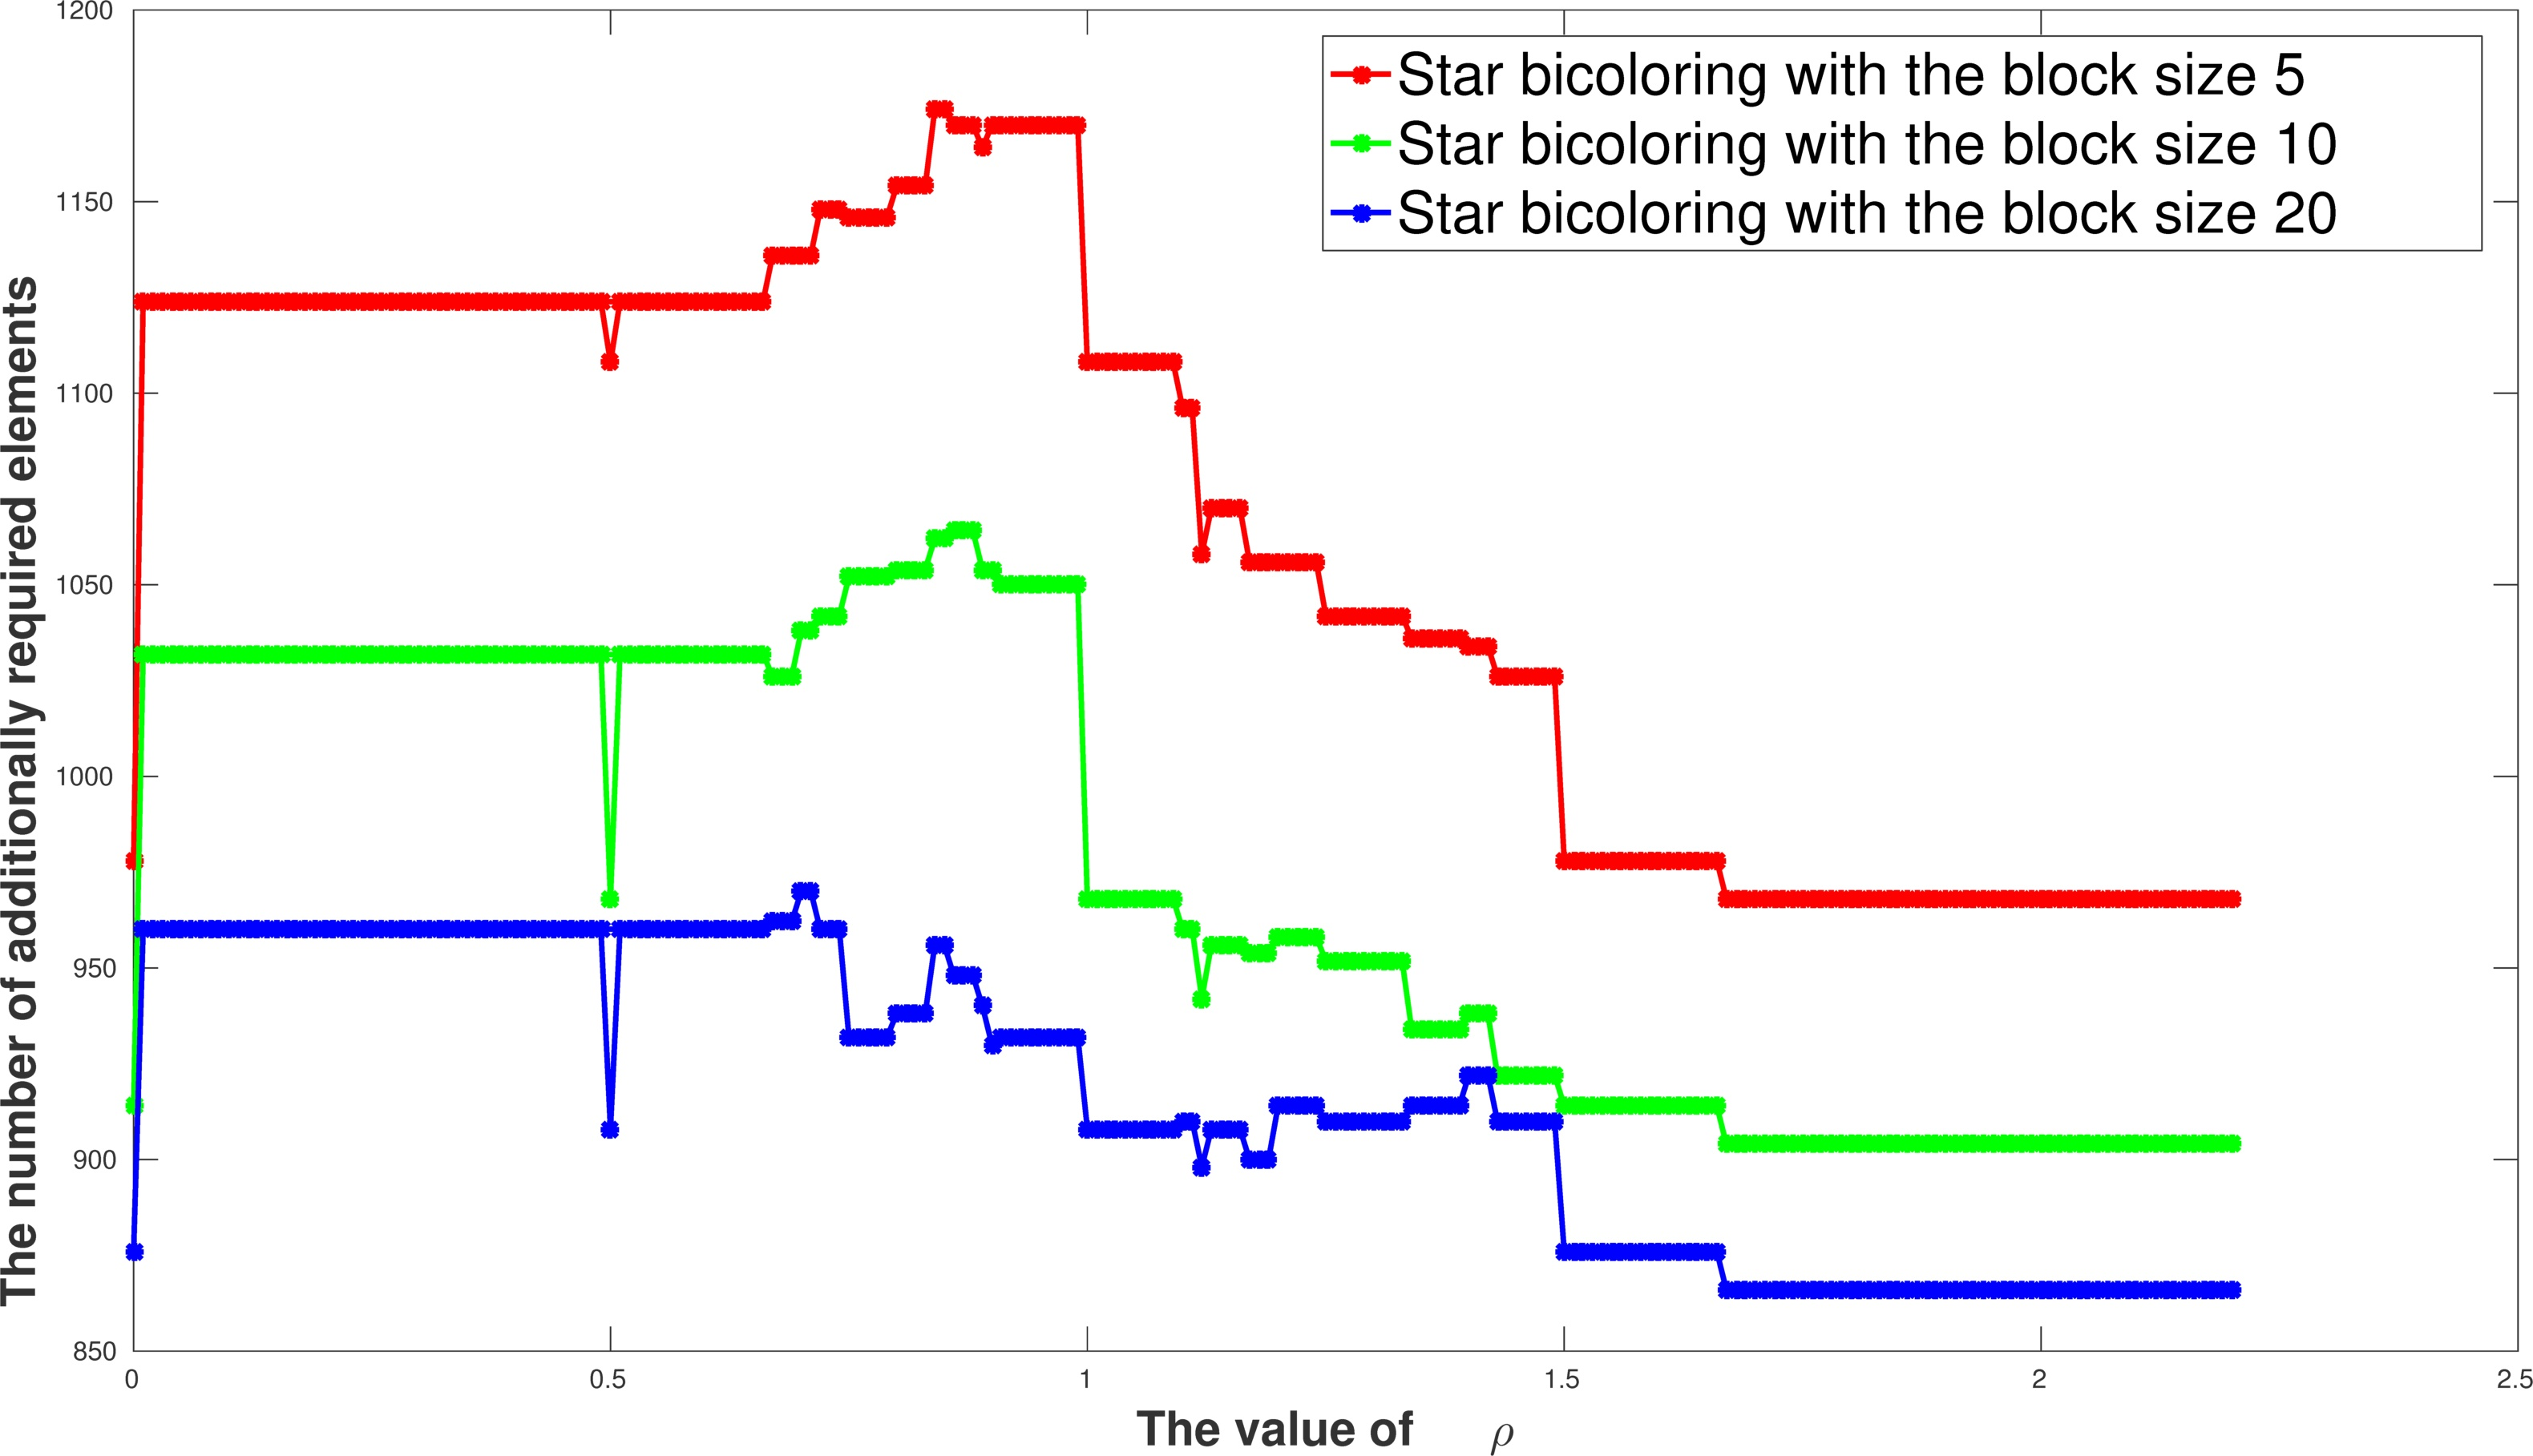
\includegraphics[width=0.9\linewidth]{rho_value_685_bus}
\caption{The influence of $\rho$ is computed on the additionally required elements
for the matrix \textit{685\_bus} with the LFO ordering.}
\label{rho_value_685_bus}
\end{figure}

\begin{figure}
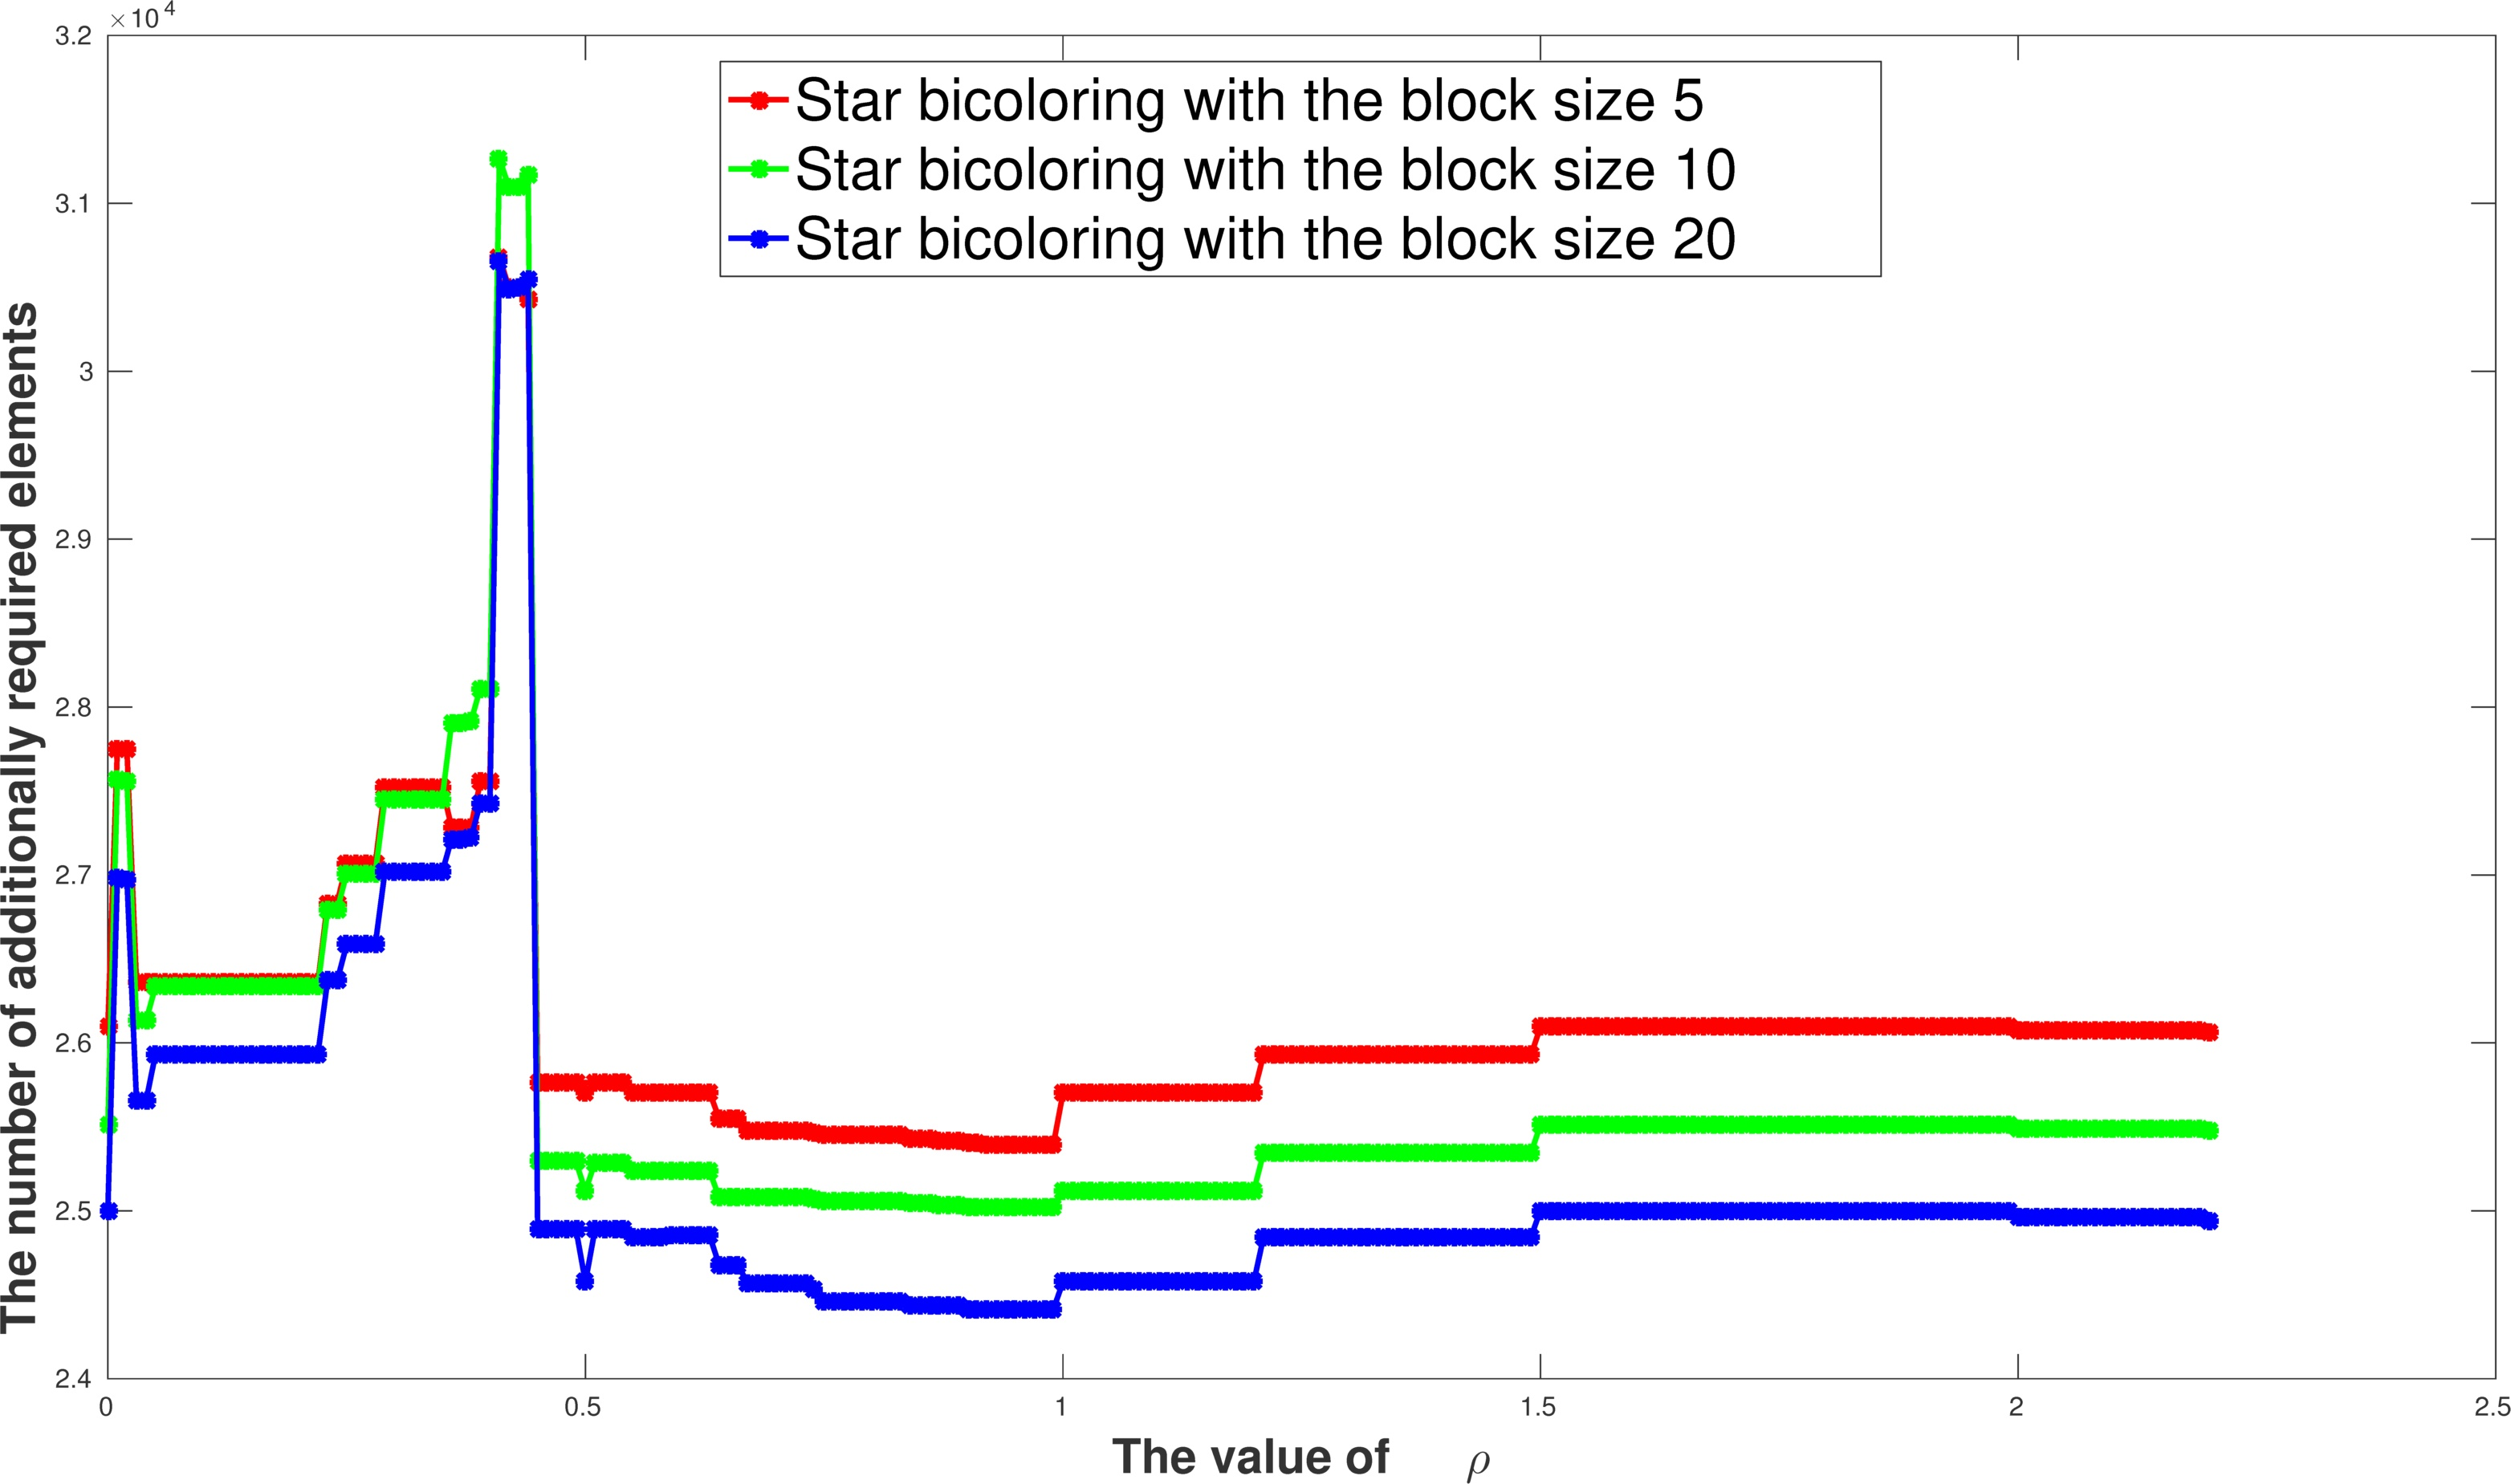
\includegraphics[width=0.9\linewidth]{rho_value_orani678}
\caption{The influence of $\rho$ is computed on the additionally required elements
for the matrix \textit{orani678} with the LFO ordering.}
\label{rho_value_orani678}
\end{figure}

Now, we introduce our new heuristic  which is a modification of the function \textit{next\_vertex}
of \coderef{orig.star.bicoloring}. The other parts of \coderef{orig.star.bicoloring} remain the same as
in our new heuristic.
\coderef{new.star.bicoloring} shows the new function \textit{next\_vertex\_nreq} which should be called
instead of \textit{next\_vertex} to get the next vertex in each step.
The global variable $NonReq$ switches between two modes in the new function \textit{next\_vertex\_nreq}.
The first mode $NonReq=false$ selects the vertex
based on the variable $\rho$ like \coderef{orig.star.bicoloring}.
The second mode $NonReq=true$ selects
the next vertex with the maximum number of determined nonrequired elements
and the minimum number of required elements.
Consider that $v$ is always computed in the first line of the function \textit{next\_vertex\_nreq}
but it will be modified later when $NonReq$ is equal to $true$.

Table~\ref{mats.pot.add.gr.vs.nreq.star} shows the numbers of potentially and additionally required elements
computed with \coderef{orig.star.bicoloring} and \coderef{new.star.bicoloring}.
Except for the matrix \textit{coater01} with the natural ordering,
we have an overall increase in both potentially and additionally required elements using \coderef{new.star.bicoloring}.
Also, \figref{crystm01_alg36_bls_nat_adds} and \figref{crystm01_alg36_bls_nat_cols} represent the computation of
\coderef{orig.star.bicoloring} and \coderef{new.star.bicoloring} while the size of blocks is changing from $1$ to $70$.
Again, an overall increase in the number of additionally required elements is achieved while the number of colors
does not increase dramatically.

\begin{table}
\centering
\begin{tabular}{|c|c|c|c|c|}
\hline
Matrix (NAT) & \multicolumn{2}{c|}{$|R_p|$} & \multicolumn{2}{c|}{$|R_a|$}\\\hline
{} & \coderef{orig.star.bicoloring} & \coderef{new.star.bicoloring} & \coderef{orig.star.bicoloring} & \coderef{new.star.bicoloring}\\\hline
\textit{steam1.mtx} & $64$ & $590$ & $64$ & $454$ \\\hline
\textit{steam2.mtx} & $240$ & $2352$ & $240$ & $1648$ \\\hline
\textit{nos3.mtx} & $4590$ & $4614$ & $2986$ & $3050$ \\\hline
\textit{ex7.mtx} & $35690$ & $36486$ & $28028$ & $28796$ \\\hline
\textit{ex33.mtx} & $9282$ & $11180$ & $6220$ & $7510$ \\\hline
\textit{crystm01.mtx} & $19262$ & $22716$ & $11472$ & $13978$ \\\hline
\textit{coater1.mtx} & $14402$ & $14442$ & $8296$ & $8262$ \\\hline
\textit{pesa.mtx} & $40572$ & $41460$ & $32728$ & $33956$ \\\hline
\end{tabular}
\vspace*{1cm}\newline
\begin{tabular}{|c|c|c|c|c|}
\hline
Matrix (LFO) & \multicolumn{2}{c|}{$|R_p|$} & \multicolumn{2}{c|}{$|R_a|$}\\\hline
{} & \coderef{orig.star.bicoloring} & \coderef{new.star.bicoloring} & \coderef{orig.star.bicoloring} & \coderef{new.star.bicoloring}\\\hline
\textit{steam1.mtx} & $64$ & $802$ & $64$ & $466$ \\\hline
\textit{steam2.mtx} & $240$ & $2352$ & $240$ & $944$ \\\hline
\textit{nos3.mtx} & $4824$ & $5166$ & $3152$ & $3444$ \\\hline
\textit{ex7.mtx} & $36794$ & $37012$ & $28670$ & $28942$ \\\hline
\textit{ex33.mtx} & $11070$ & $11426$ & $7380$ & $7708$ \\\hline
\textit{crystm01.mtx} & $21420$ & $22714$ & $13012$ & $13992$ \\\hline
\textit{coater1.mtx} & $14422$ & $14496$ & $8204$ & $8350$ \\\hline
\textit{pesa.mtx} & $42758$ & $42904$ & $32272$ & $34266$ \\\hline
\end{tabular}
\vspace*{1cm}\newline
\begin{tabular}{|c|c|c|c|c|}
\hline
Matrix (SLO) & \multicolumn{2}{c|}{$|R_p|$} & \multicolumn{2}{c|}{$|R_a|$}\\\hline
{} & \coderef{orig.star.bicoloring} & \coderef{new.star.bicoloring} & \coderef{orig.star.bicoloring} & \coderef{new.star.bicoloring}\\\hline
\textit{steam1.mtx} & $64$ & $824$ & $64$ & $616$ \\\hline
\textit{steam2.mtx} & $240$ & $2320$ & $240$ & $1616$ \\\hline
\textit{nos3.mtx} & $4314$ & $4760$ & $2784$ & $3102$ \\\hline
\textit{ex7.mtx} & $35690$ & $36450$ & $27814$ & $28568$ \\\hline
\textit{ex33.mtx} & $9728$ & $10978$ & $6468$ & $7296$ \\\hline
\textit{crystm01.mtx} & $24222$ & $27226$ & $14562$ & $16590$ \\\hline
\textit{coater1.mtx} & $14532$ & $14634$ & $8194$ & $8412$ \\\hline
\textit{pesa.mtx} & $41128$ & $42112$ & $31114$ & $33744$ \\\hline
\end{tabular}
\caption{The comparison between the number of potentially and additionally required
elements computed with \coderef{orig.star.bicoloring} and \coderef{new.star.bicoloring}.
The block size is fixed to $10$. The orderings for coloring are (Top) the natural ordering,
(Middle) LFO, and (Bottom) SLO.}
\label{mats.pot.add.gr.vs.nreq.star}
\end{table}


\begin{figure}
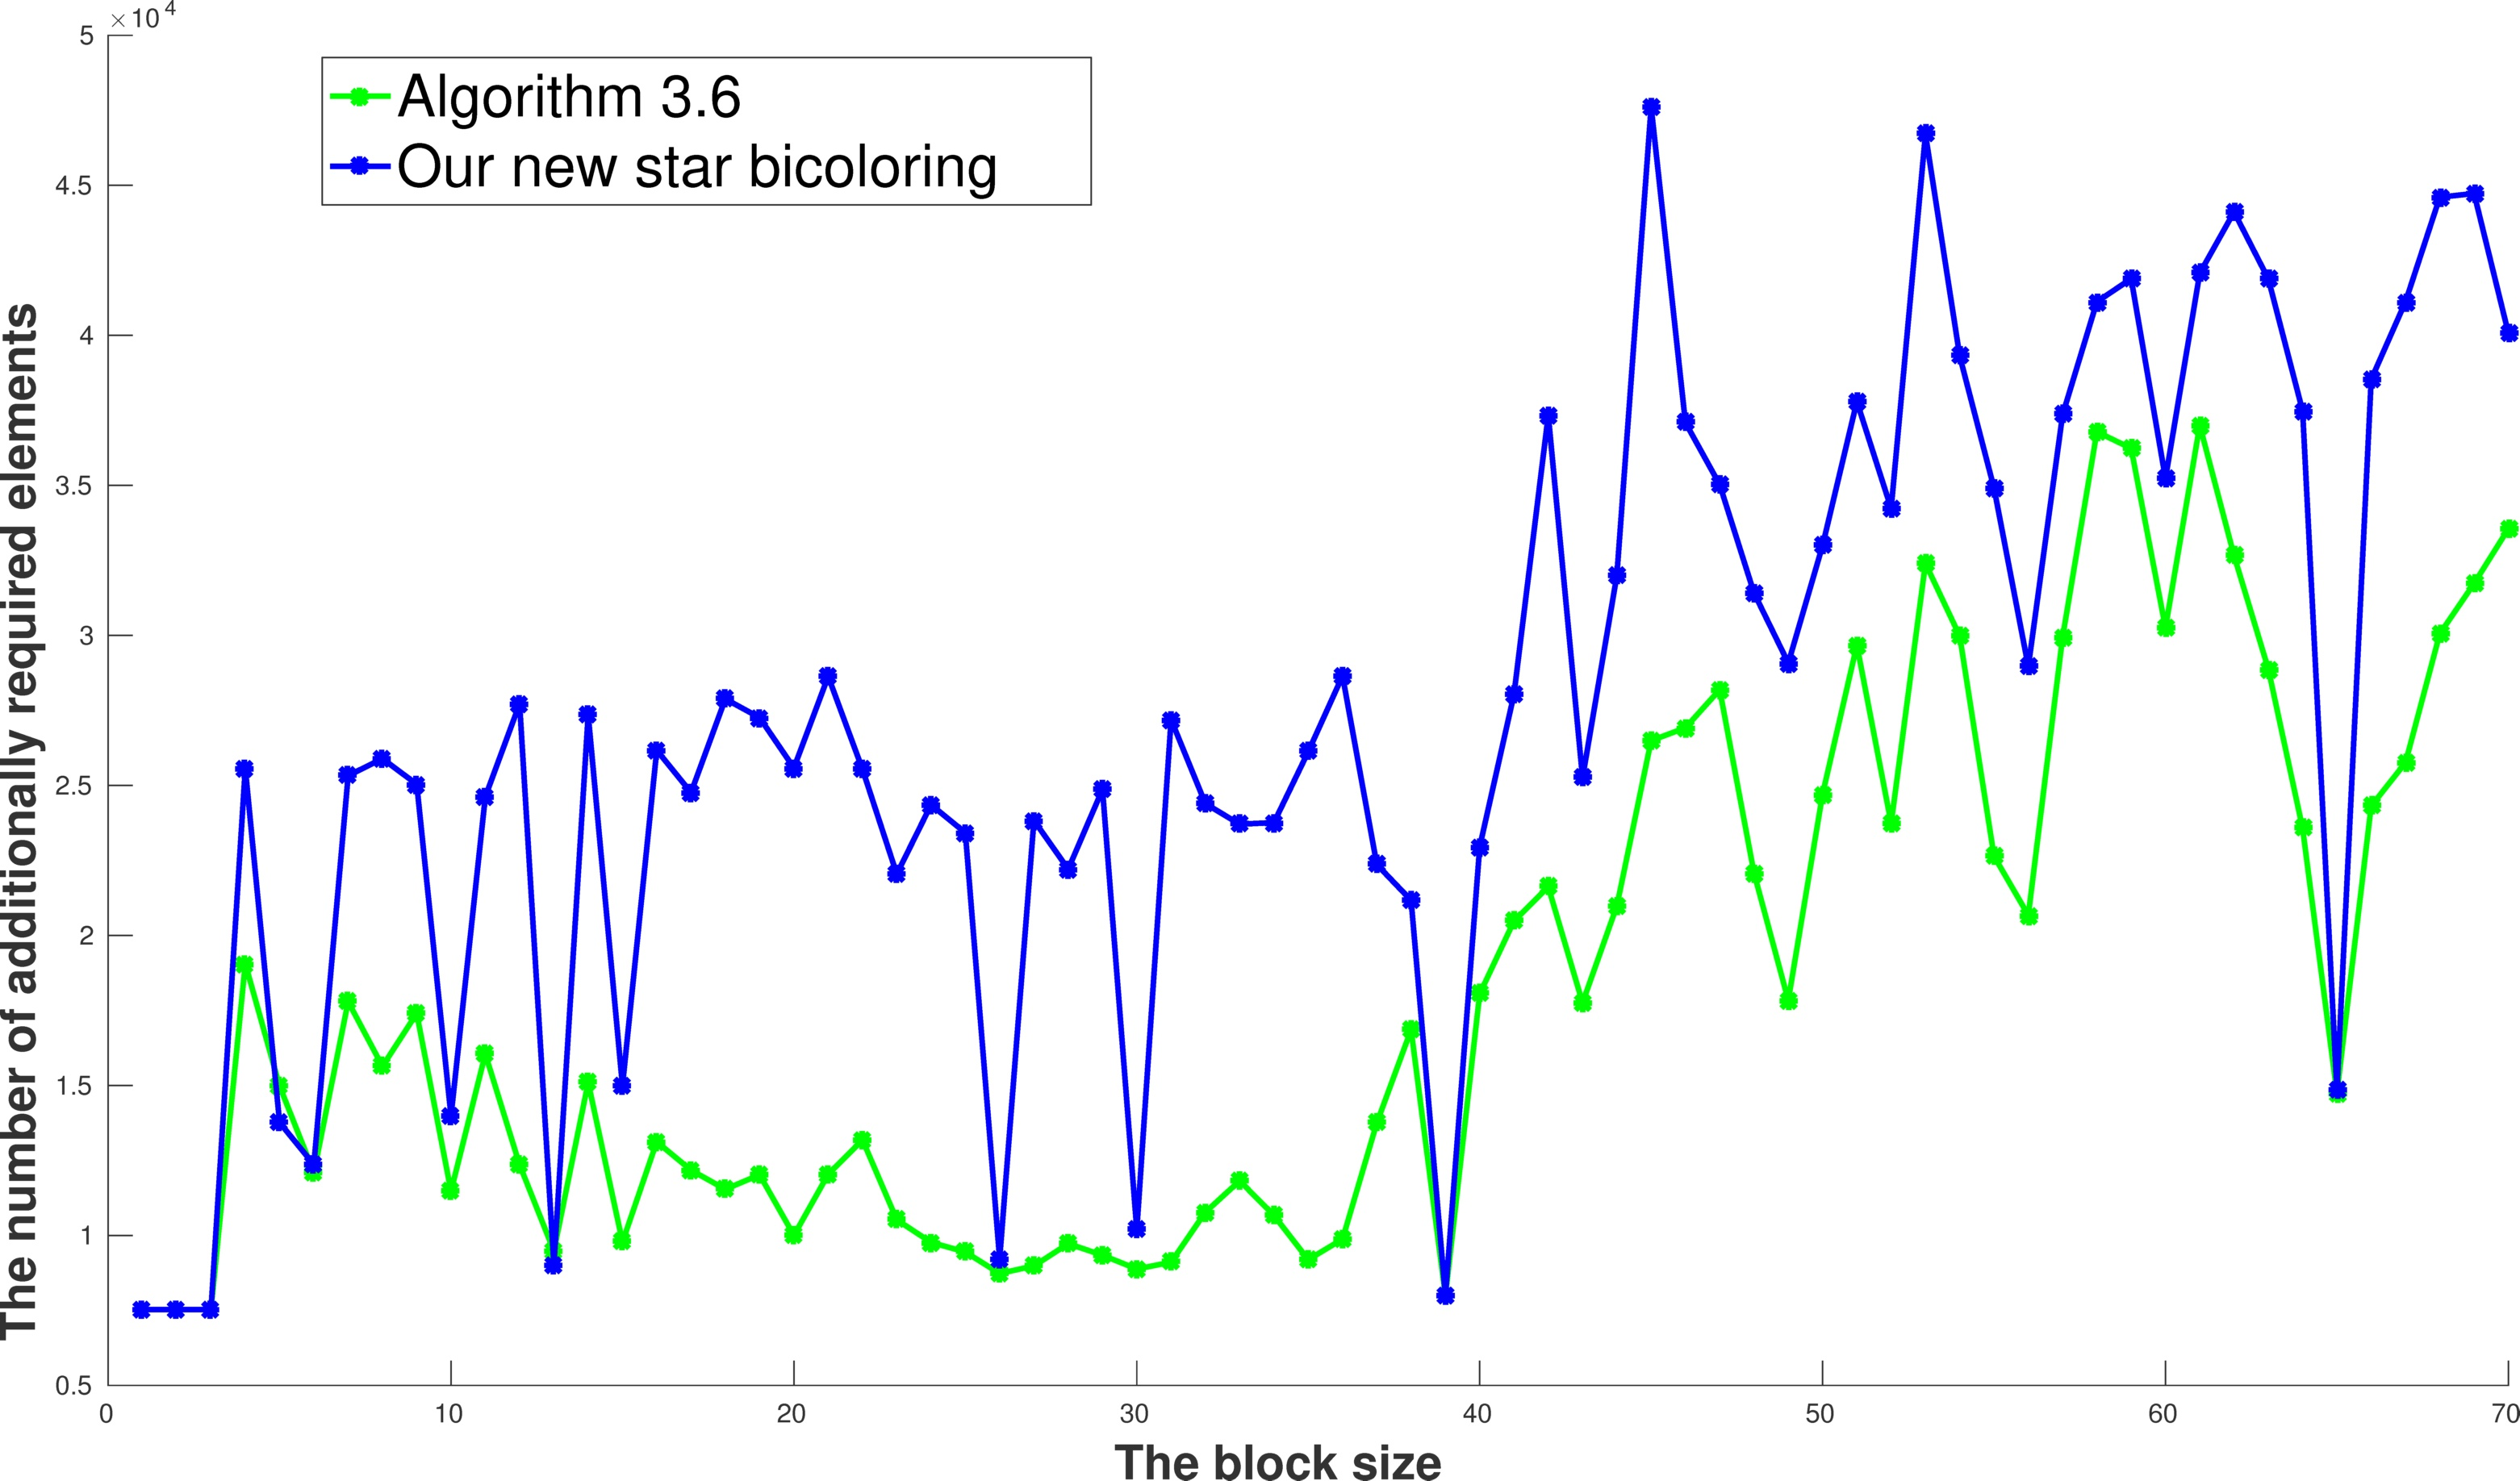
\includegraphics[width=0.9\linewidth]{crystm01_alg36_bls_nat_adds}
\caption{The number of additionally required elements computed with
\coderef{new.star.bicoloring} compared with \coderef{orig.star.bicoloring}.
The nonsymmetric matrix \textit{$crystm01$} with the natural ordering is used here.}
\label{crystm01_alg36_bls_nat_adds}

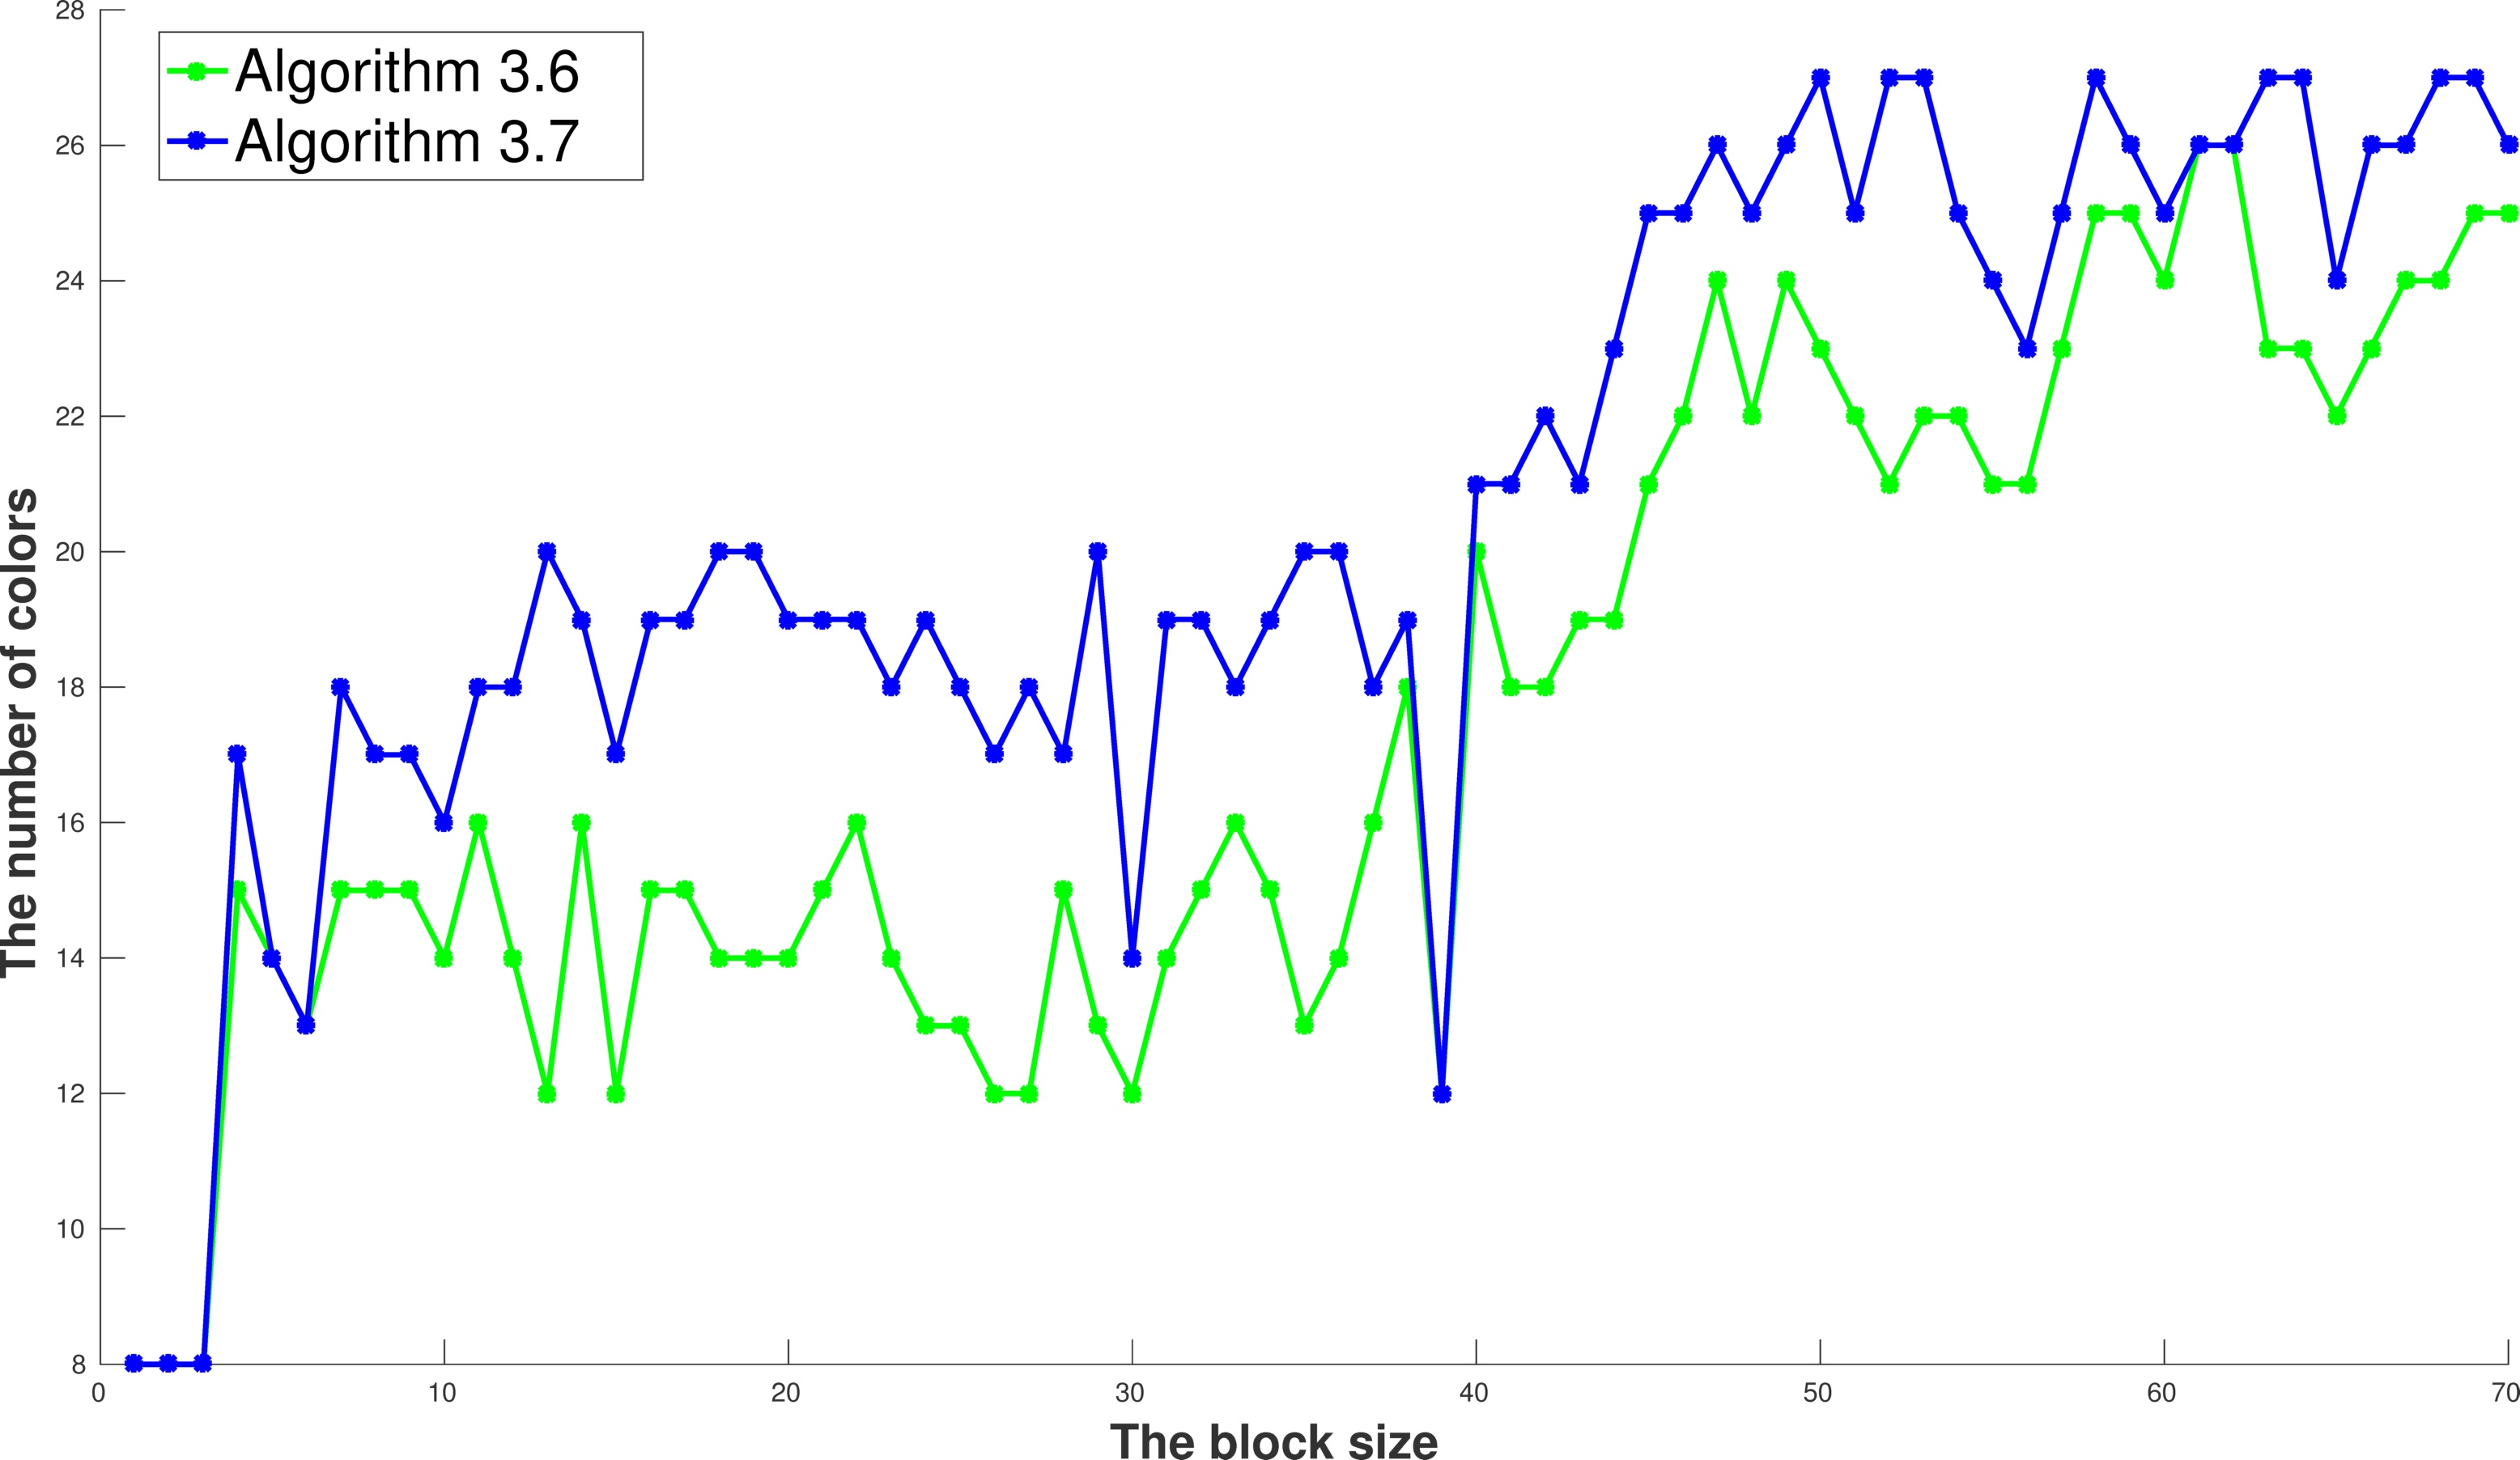
\includegraphics[width=0.9\linewidth]{crystm01_alg36_bls_nat_cols}
\caption{The number of colors computed with
\coderef{new.star.bicoloring} compared with \coderef{orig.star.bicoloring}.
The nonsymmetric matrix \textit{$crystm01$} with the natural ordering is used here.}
\label{crystm01_alg36_bls_nat_cols}
\end{figure}


%\begin{figure}
%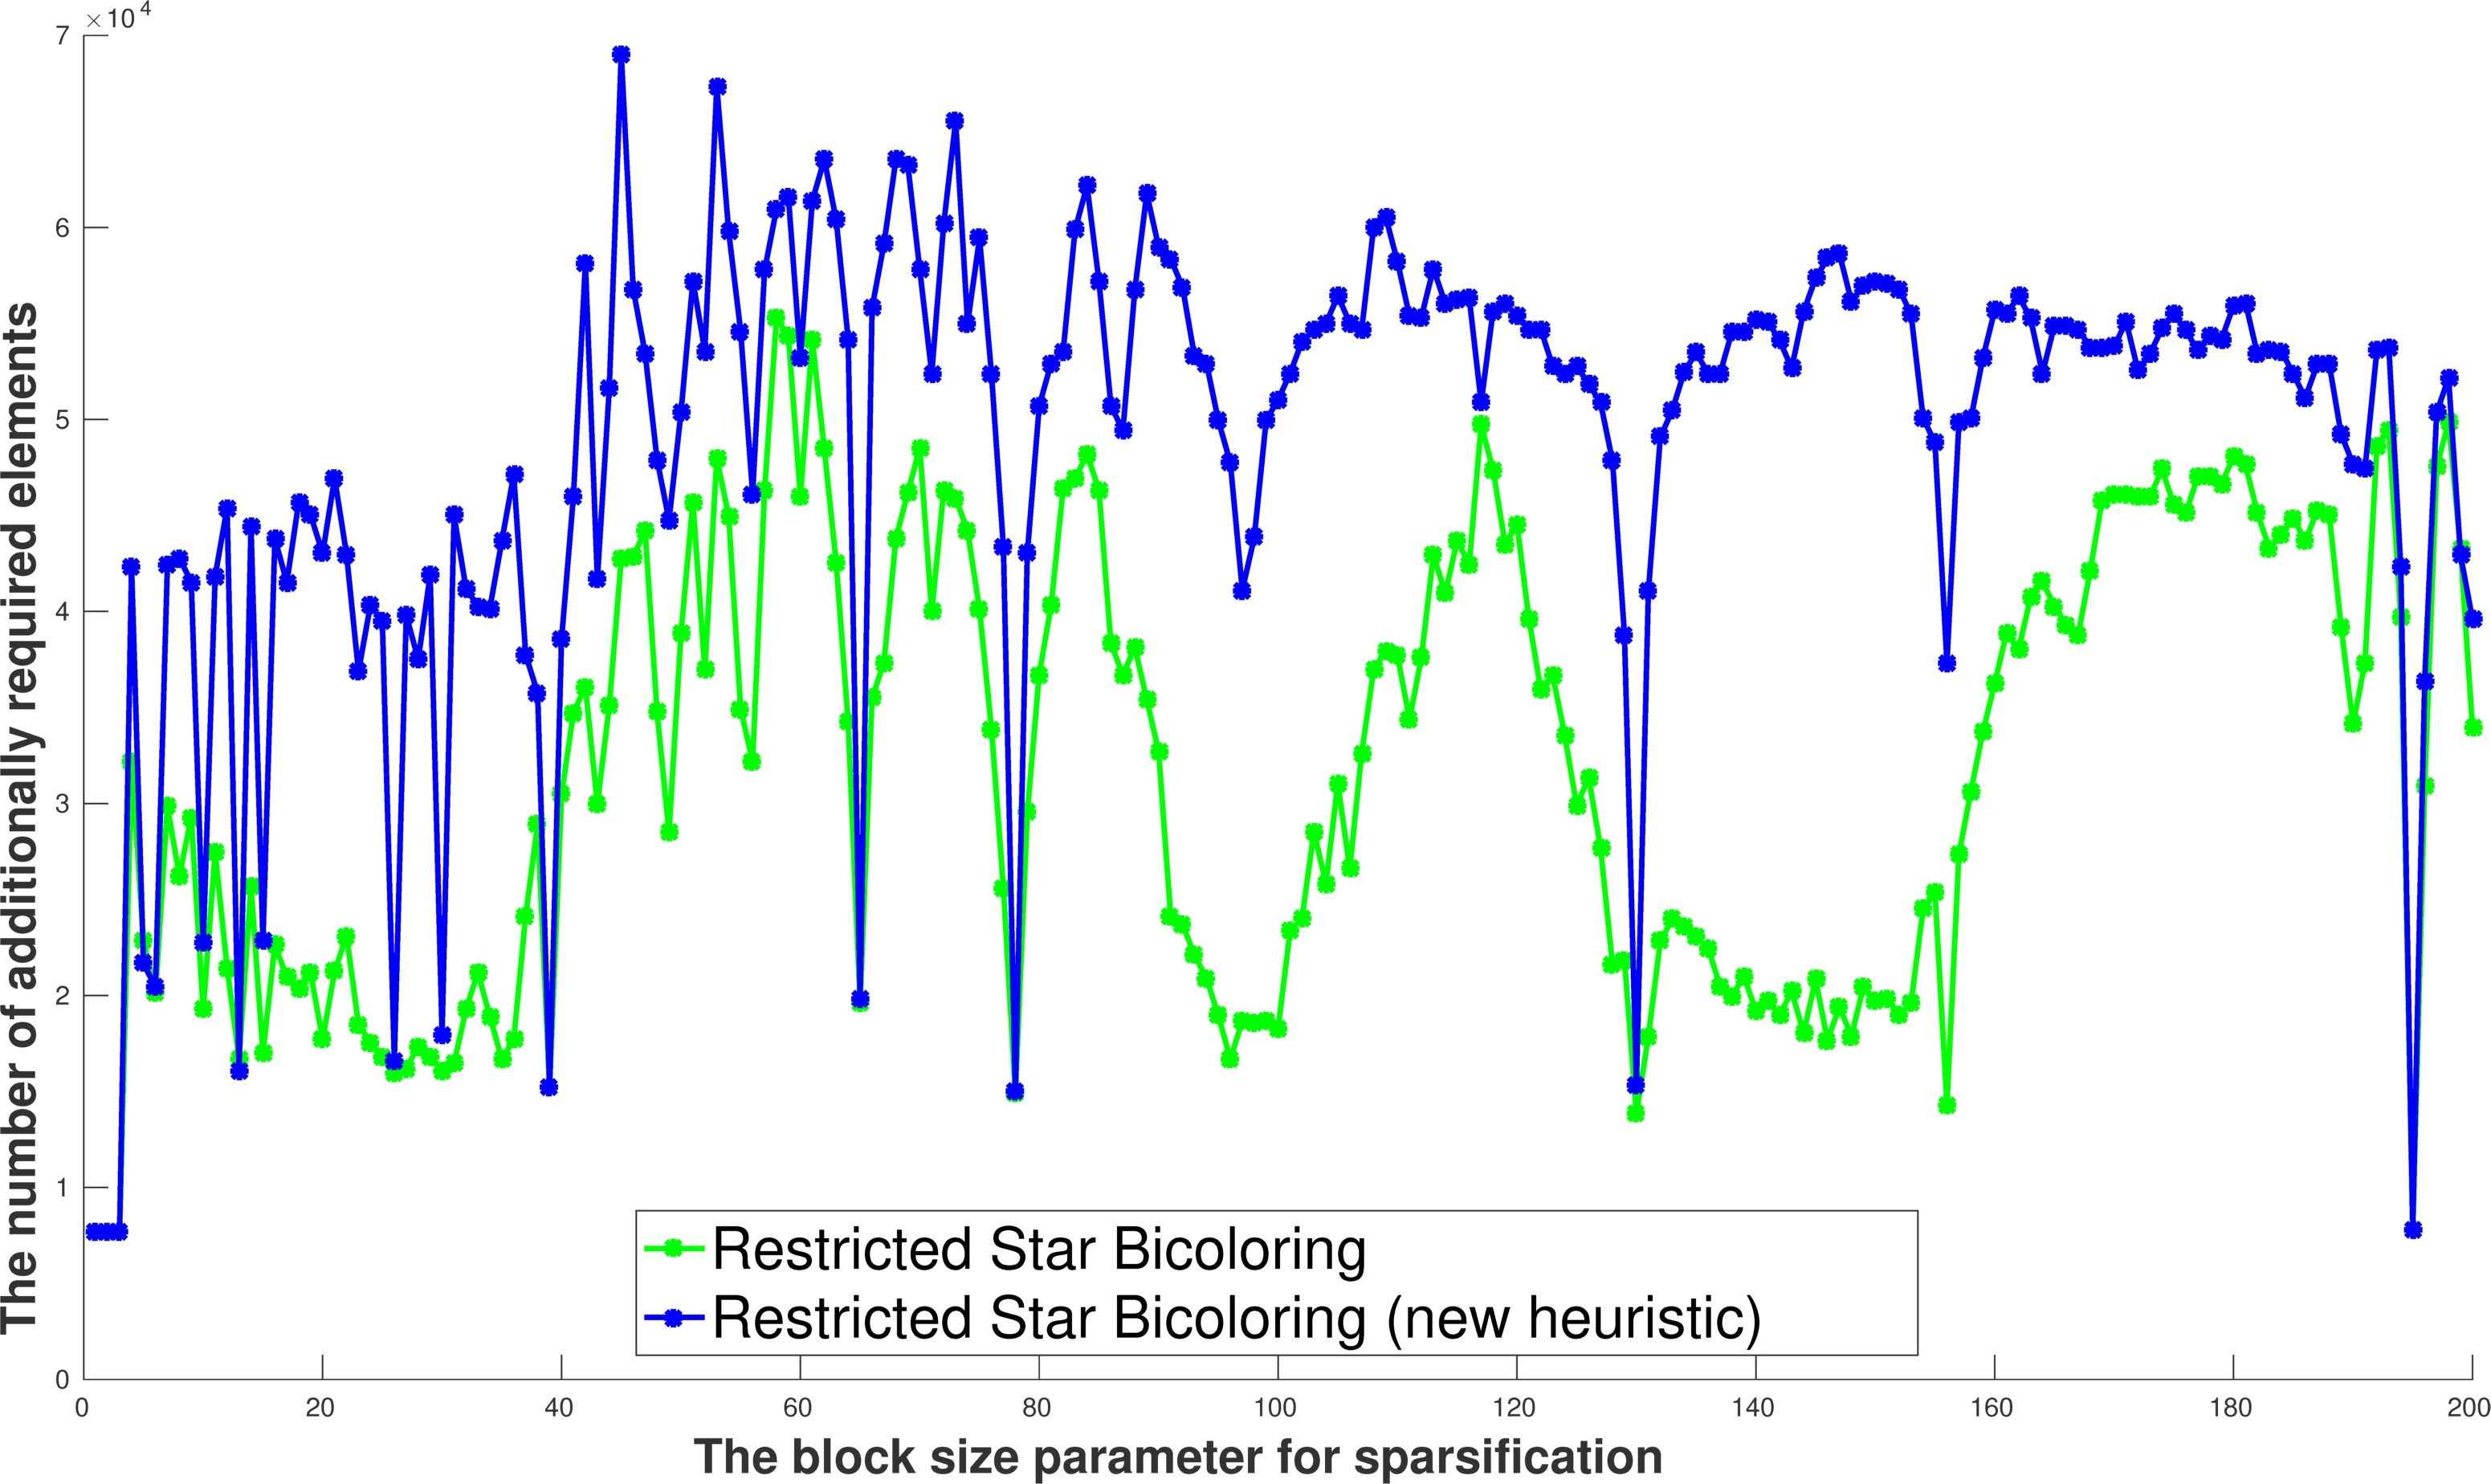
\includegraphics[width=\linewidth]{bls_adds_crystm01_old_star_vs_new}
%\caption{The number of additionally required elements computed with
%the new star bicoloring compared with the older implementation.
%The nonsymmetric matrix \textit{$crystm01$} is used here.}
%\label{bls_adds_crystm01_old_star_vs_new}
%\end{figure}

%\begin{figure}
%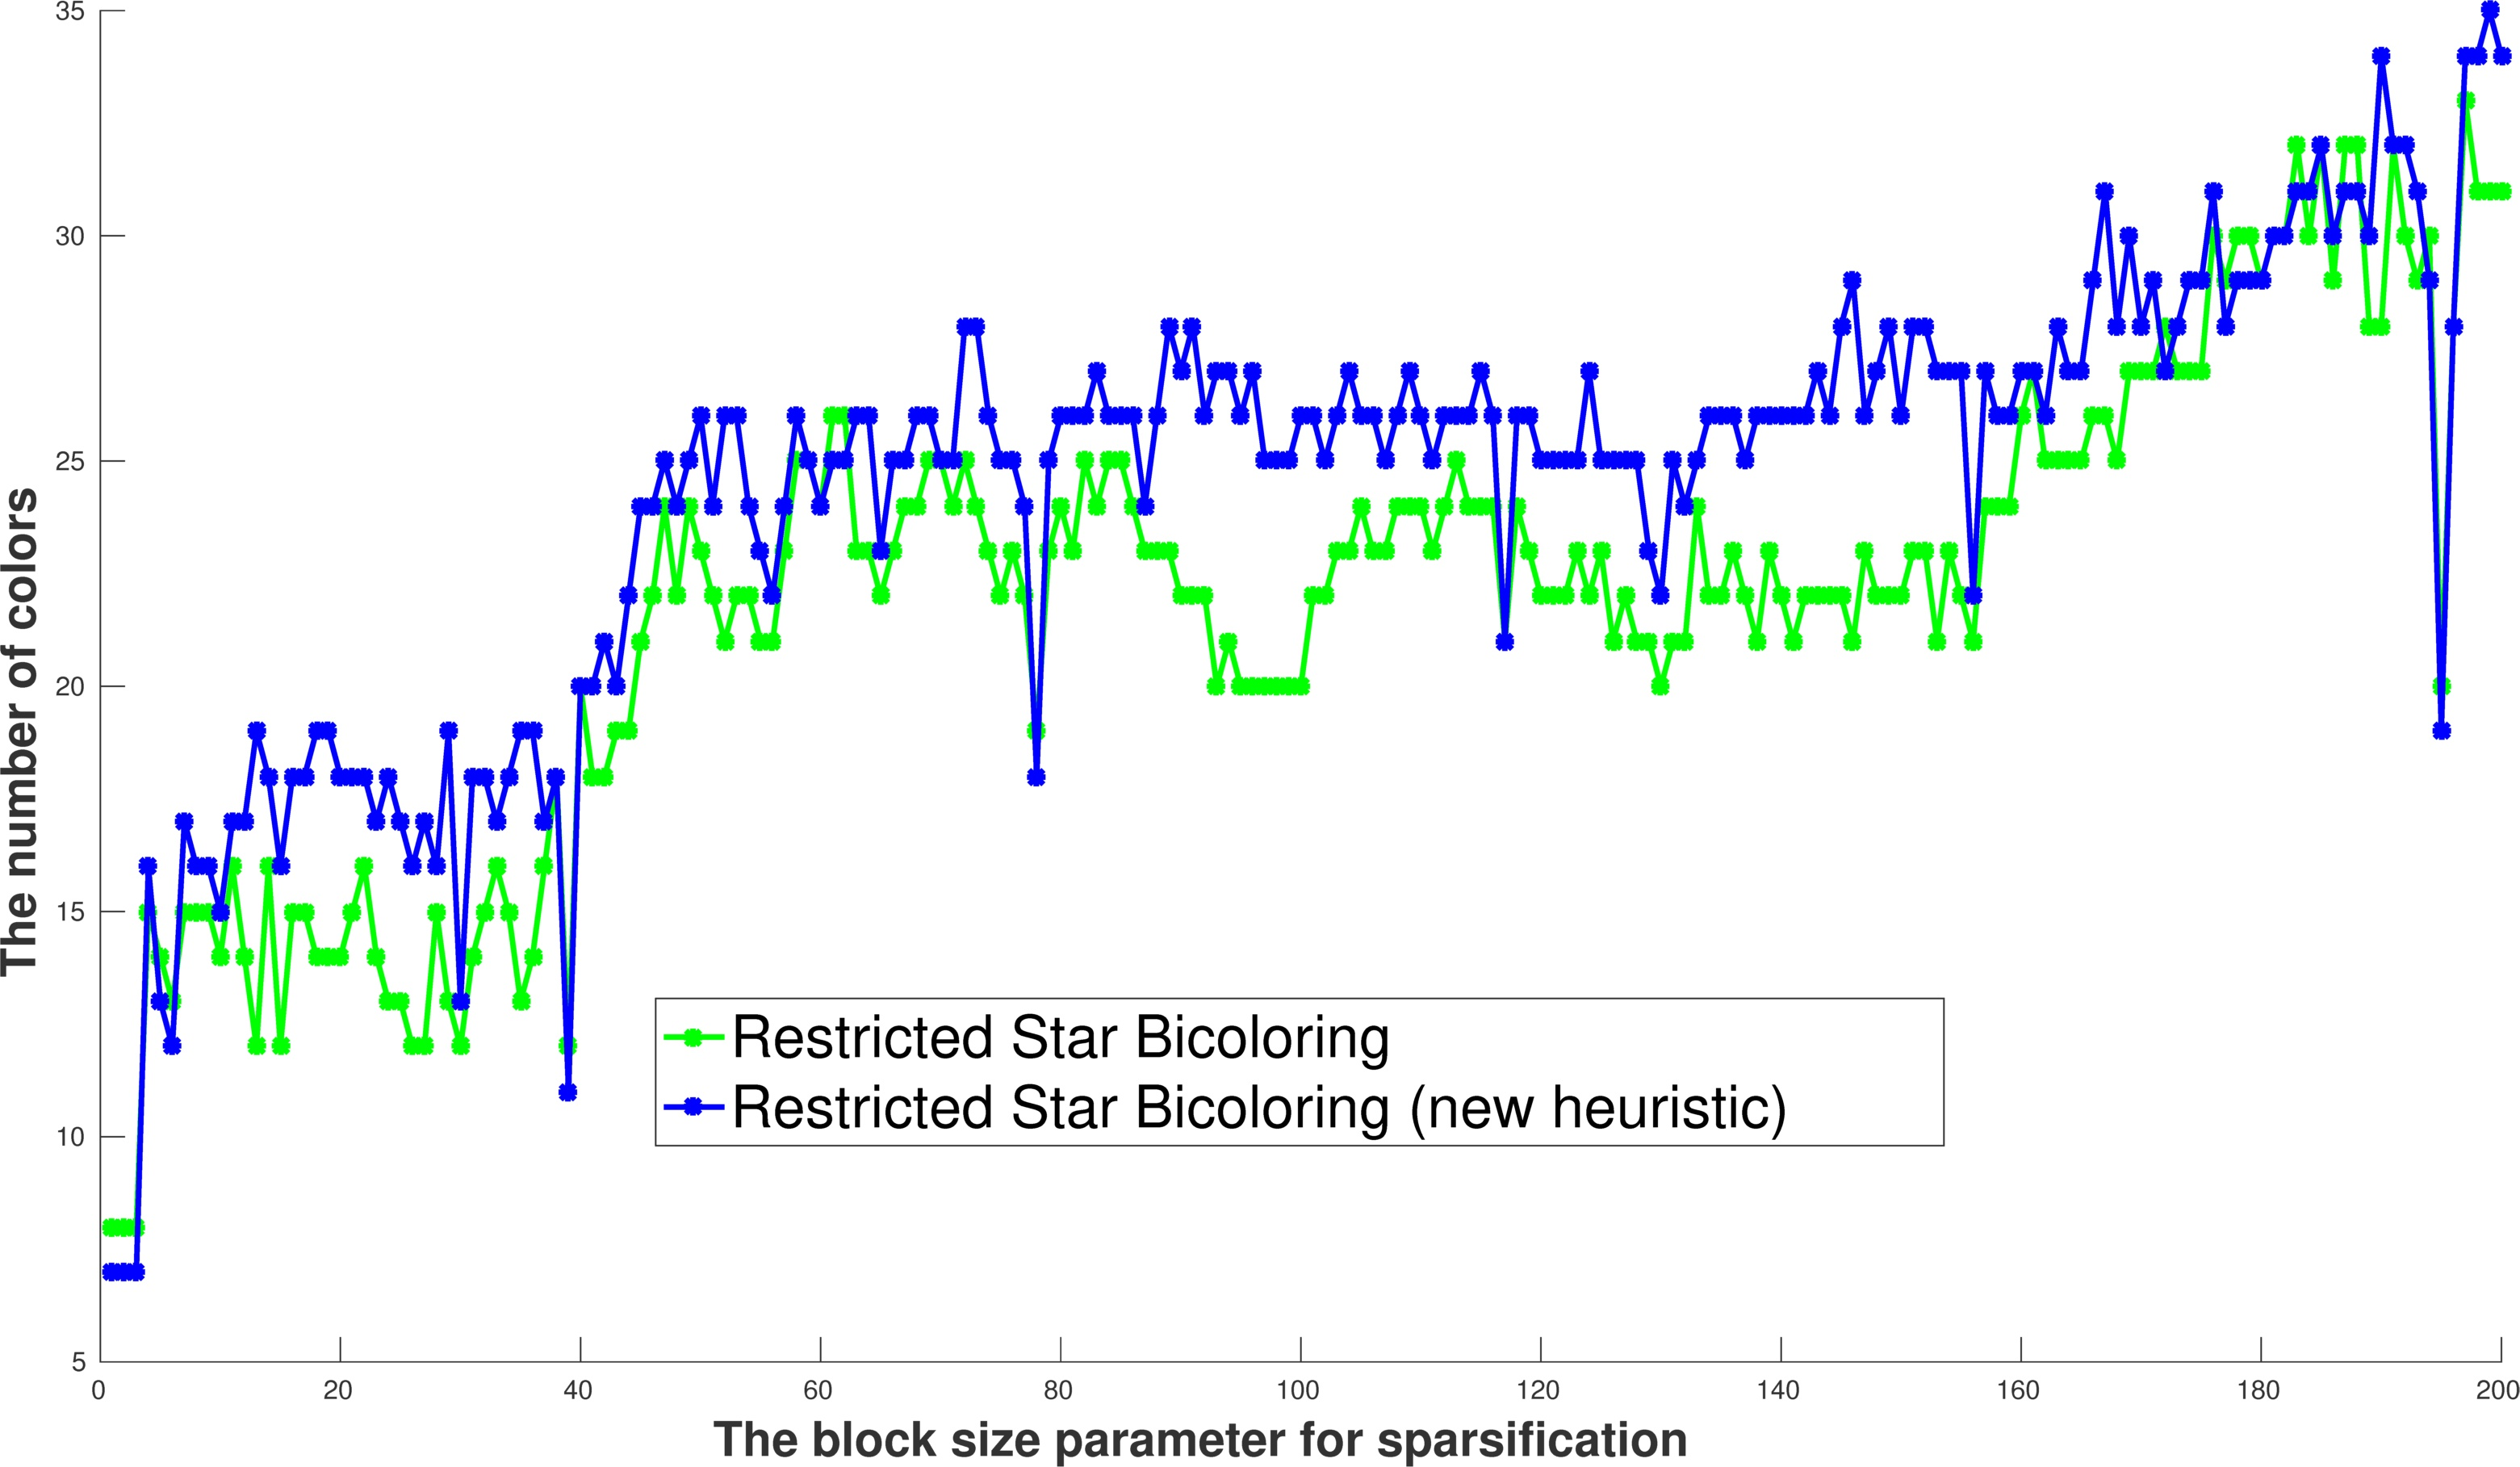
\includegraphics[width=\linewidth]{bls_cols_crystm01_old_star_vs_new}
%\caption{The number of additionally required elements computed with
%the new star bicoloring compared with the older implementation.
%The nonsymmetric matrix \textit{$crystm01$} is used here.}
%\label{bls_cols_crystm01_old_star_vs_new}
%\end{figure}

%\cite{mpi_greedy_coloring}

%%%%%%%%%%%%%%%%%%%%%%%%%%%%%%%%%%%%%%%%%%%%%%%%%%%%%%%%%%%%%%%%%%%%%%%%%%%%%%%%%%%%%%%%%%%%%%
\clearpage
\section{Application in geoscience}
\label{s.application}
%%%%%%%%%%%%%%%%%%%%%%%%%%%%%%%%%%%%%%%%%%%%%%%%%%%%%%%%%%%%%%%%%%%%%%%%%%%%%%%%%%%%%%%%%%%%%%
Here, we apply our new heuristics to a carbon sequestration example from geoscience.
The geophysics group of RWTH Aachen simulates the injection of CO\textsubscript{2}
in a reservoir by a two-phase flow model in porous media. These two phases are a wetting
and non-wetting phase like water and gas. A 2D two-phase flow can be formulated as
a system of coupled nonlinear partial differential equations in which the boundary conditions
are Dirichlet and Neumann. Integrating the time with the implicit Euler method
based on~\cite{Busing2014UEJ,Lulfesmann2012Fap} results in the following system of nonlinear equations,
$$F(u)=0 \, \text{ with } \, u = \binom{p_w}{S_n} \in \R^{2MN} \, \text{ and } \, F = \binom{F_1}{F_2} \in \R^{2MN},$$
where the variable $p_w \in \R^{MN}$ is the pressure for the wetting phase and $S_n \in \R^{MN}$ is the non-wetting saturation. The Newton's method solves this system of equations.
Hence, the $2MN \times 2MN$ Jacobian matrix
$$
A =
\left({\begin{array}{l|l}
	\displaystyle \frac{\partial F_1}{\partial p_w} & \displaystyle \frac{\partial F_1}{\partial S_n} \\[1em]
	\hline
	\displaystyle \frac{\partial F_2}{\partial p_w} \rule[-7.5pt]{0pt}{30pt} & \displaystyle \frac{\partial F_2}{\partial S_n} \\
 \end{array}} \right).
$$
is determined with an AD-transformed version of the original function $F$. The AD tool \mbox{ADiMat}~\cite{Bischof2002CST,Willkomm2014ANU} is used for this transformation.

This Jacobian matrix is divided into four quadrants: the derivative $\partial F_1 / \partial p_w$ in the top left quadrant, $\partial F_1 / \partial S_n$ in the top right, $\partial F_2 / \partial p_w$ in the bottom left, and $\partial F_2 / \partial S_n$ in the bottom right. Arising from a particular discretization,
the sparsity patterns of the $462 \times 462$ Jacobian matrix $A$
with $3,236$ nonzeros is depicted in \figref{f:geophysik_J_matrices}.
The discretization uses different stencils resulting in different sparsity patterns of quadrants.
The Jacobian matrix
$$
A =
\left({\begin{array}{l|l}
	\text{five-point stencil} & \text{two-point stencil} \\[0.25em]
	\hline
	\text{five-point stencil} \rule[-7.5pt]{0pt}{21pt} & \text{five-point stencil} \\
 \end{array}} \right)
\quad.
$$
is based on the five-point stencil
in the north west, south east, and south west quadrant.
In the north east, the two-point stencil~$\{(m,n), (m,n-1)\}$ with the center~$(m,n)$ is used.
More details are found in \cite{Lulfesmann2012Fap}.

\begin{figure}%
	\footnotesize
	\centering
         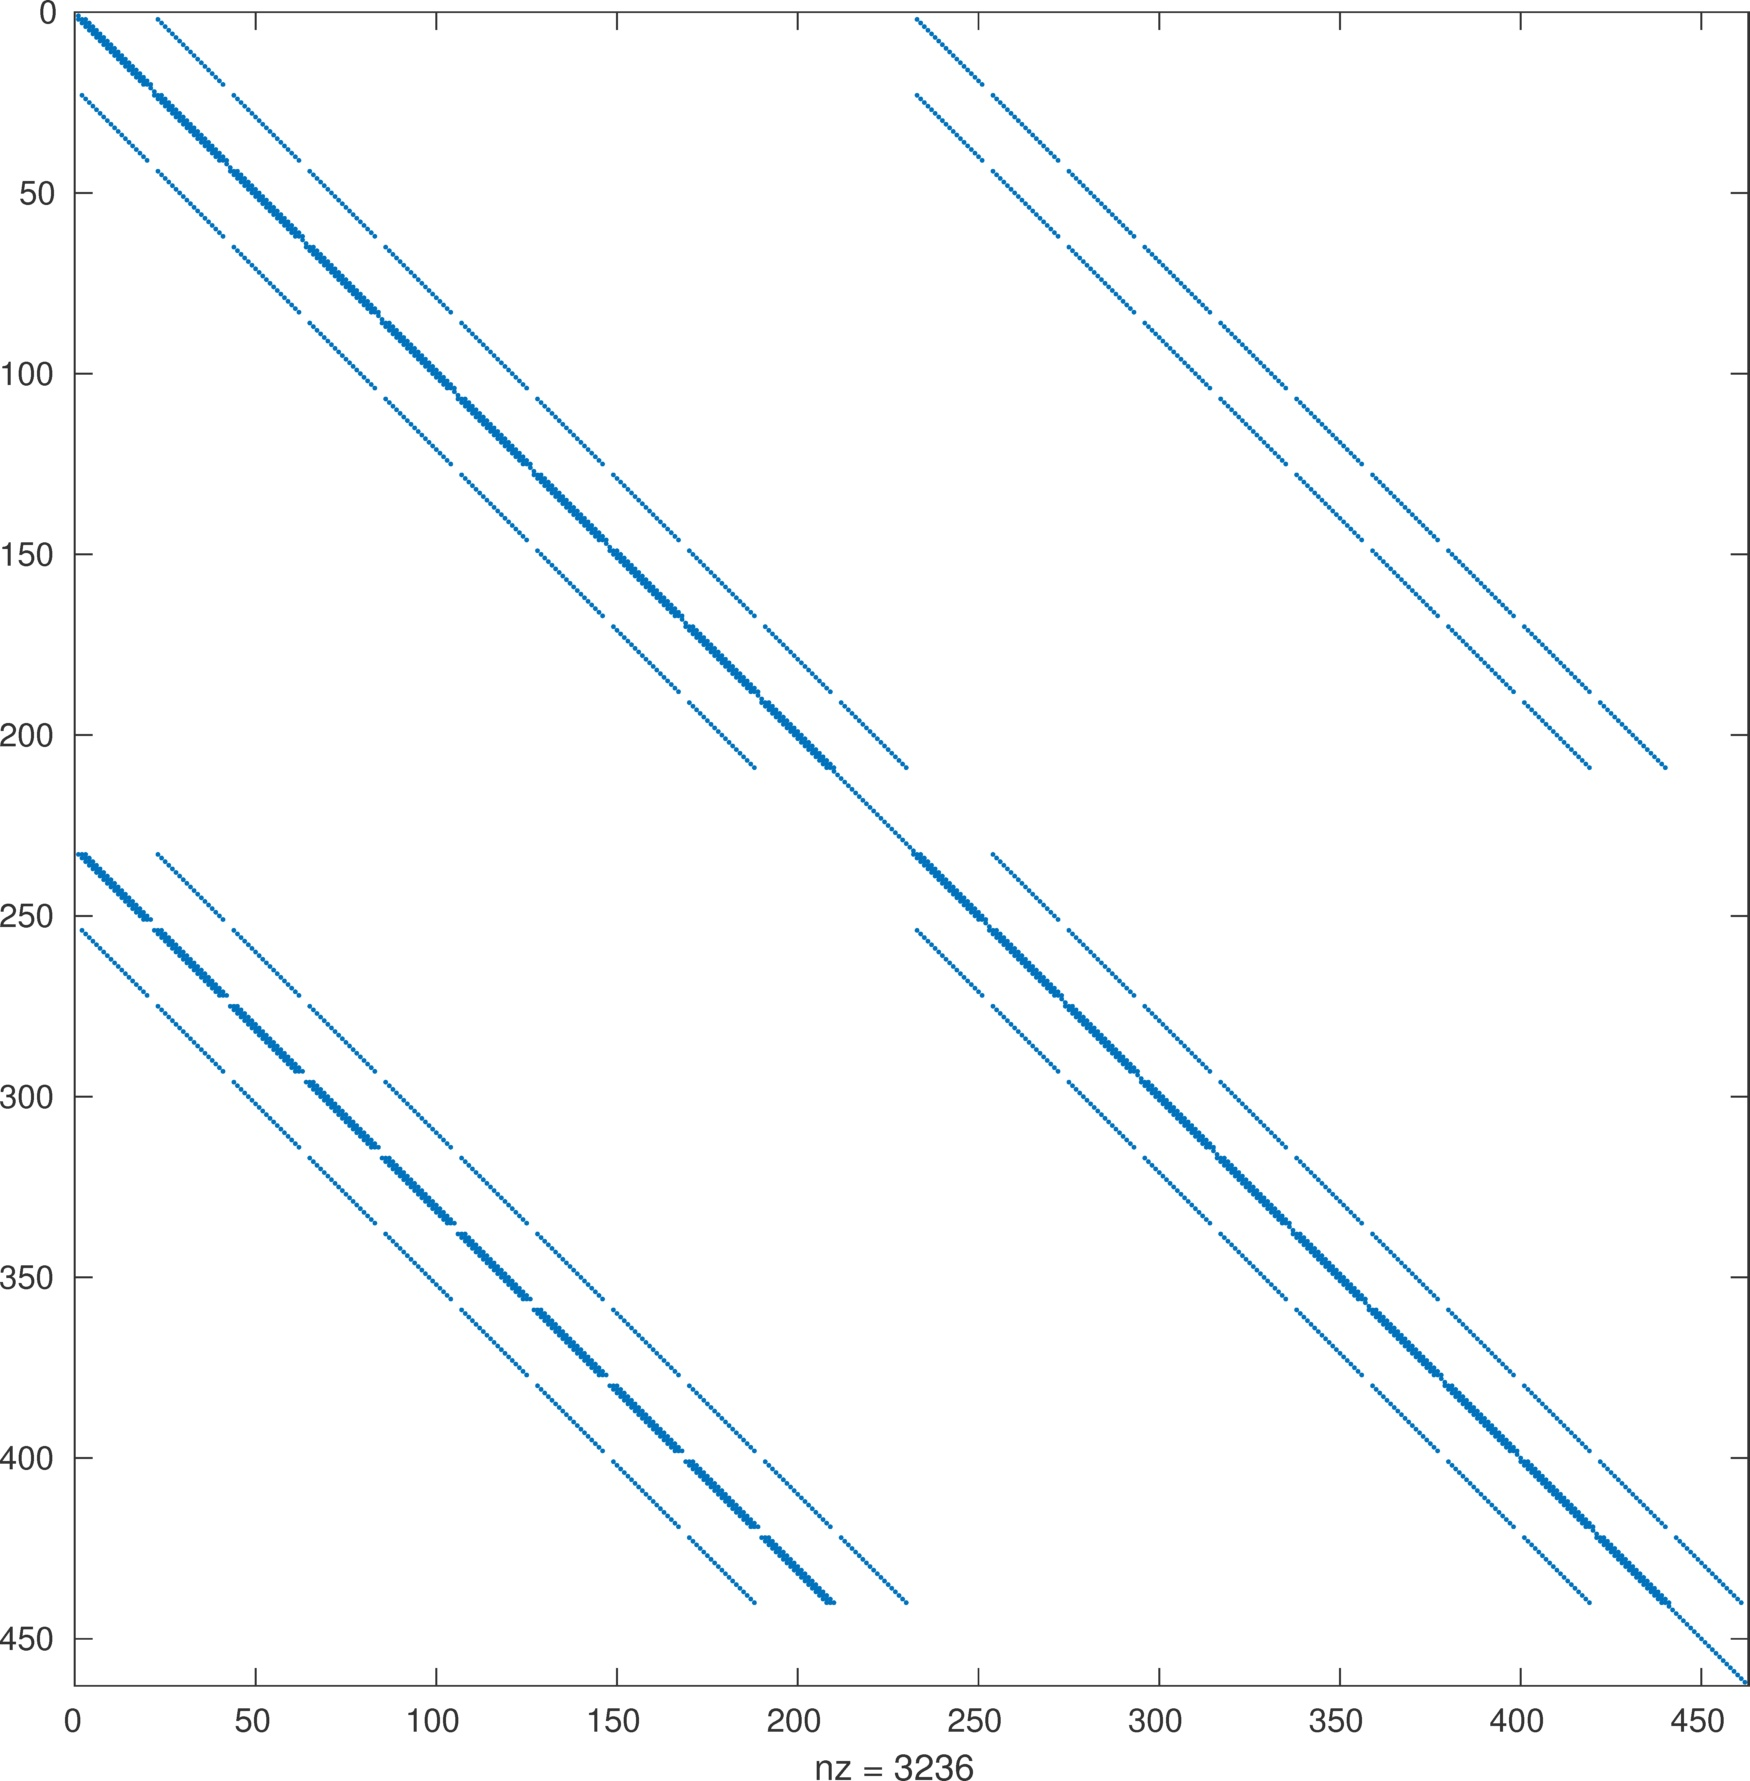
\includegraphics[width=0.6\linewidth]{co2_jac}
\caption{Sparsity pattern of Jacobian matrix~$A$.}%
\label{f:geophysik_J_matrices}
\end{figure}

We solve the resulting systems of linear equations with the
coefficient matrix $A$ in MATLAB using the BICGSTAB iterative solver.
The right-hand side is the sum of all columns.
We compute the ILU($2$) preconditioning on a set of selected elements $S$
instead of the whole Jacobian matrix.
We compare the convergence histories of the BICGSTAB solver
on the four different methods of preconditioning:
without preconditioning,
preconditioning with $S=R_i$,
preconditioning with $S=R_i + R_a$ in which
the set $R_a$ is computed based on the greedy coloring in\coderef{code.greedy},
and preconditioning with $S=R_i + R_a$ in which
the set $R_a$ is computed based on the our proposed modified greedy coloring in \coderef{code.new.impr2}.

We do this comparison for four block sizes $5$,$10$,$15$, and $20$ in
\figref{f.convergence_greedy_new2} and \figref{f.convergence_greedy_new3}.
In all of these block sizes, the preconditisoning computed based
on the new coloring converges in smaller numbers of matrix-vector products.
However, it does not mean that a bigger block size results always in a better convergence
as you can compare the figures for the blocksizes $10$ and $20$.

Table~\ref{bls.greedy.new.carbon} shows the results of the computation of \coderef{code.greedy} and
\coderef{code.new.impr2} for the different block sizes and for the Jacobian $A$.
The number of potentially and additionally required elements once more increases in all block sizes
while the number of colors tends to be the same.

\begin{figure}
\centering
%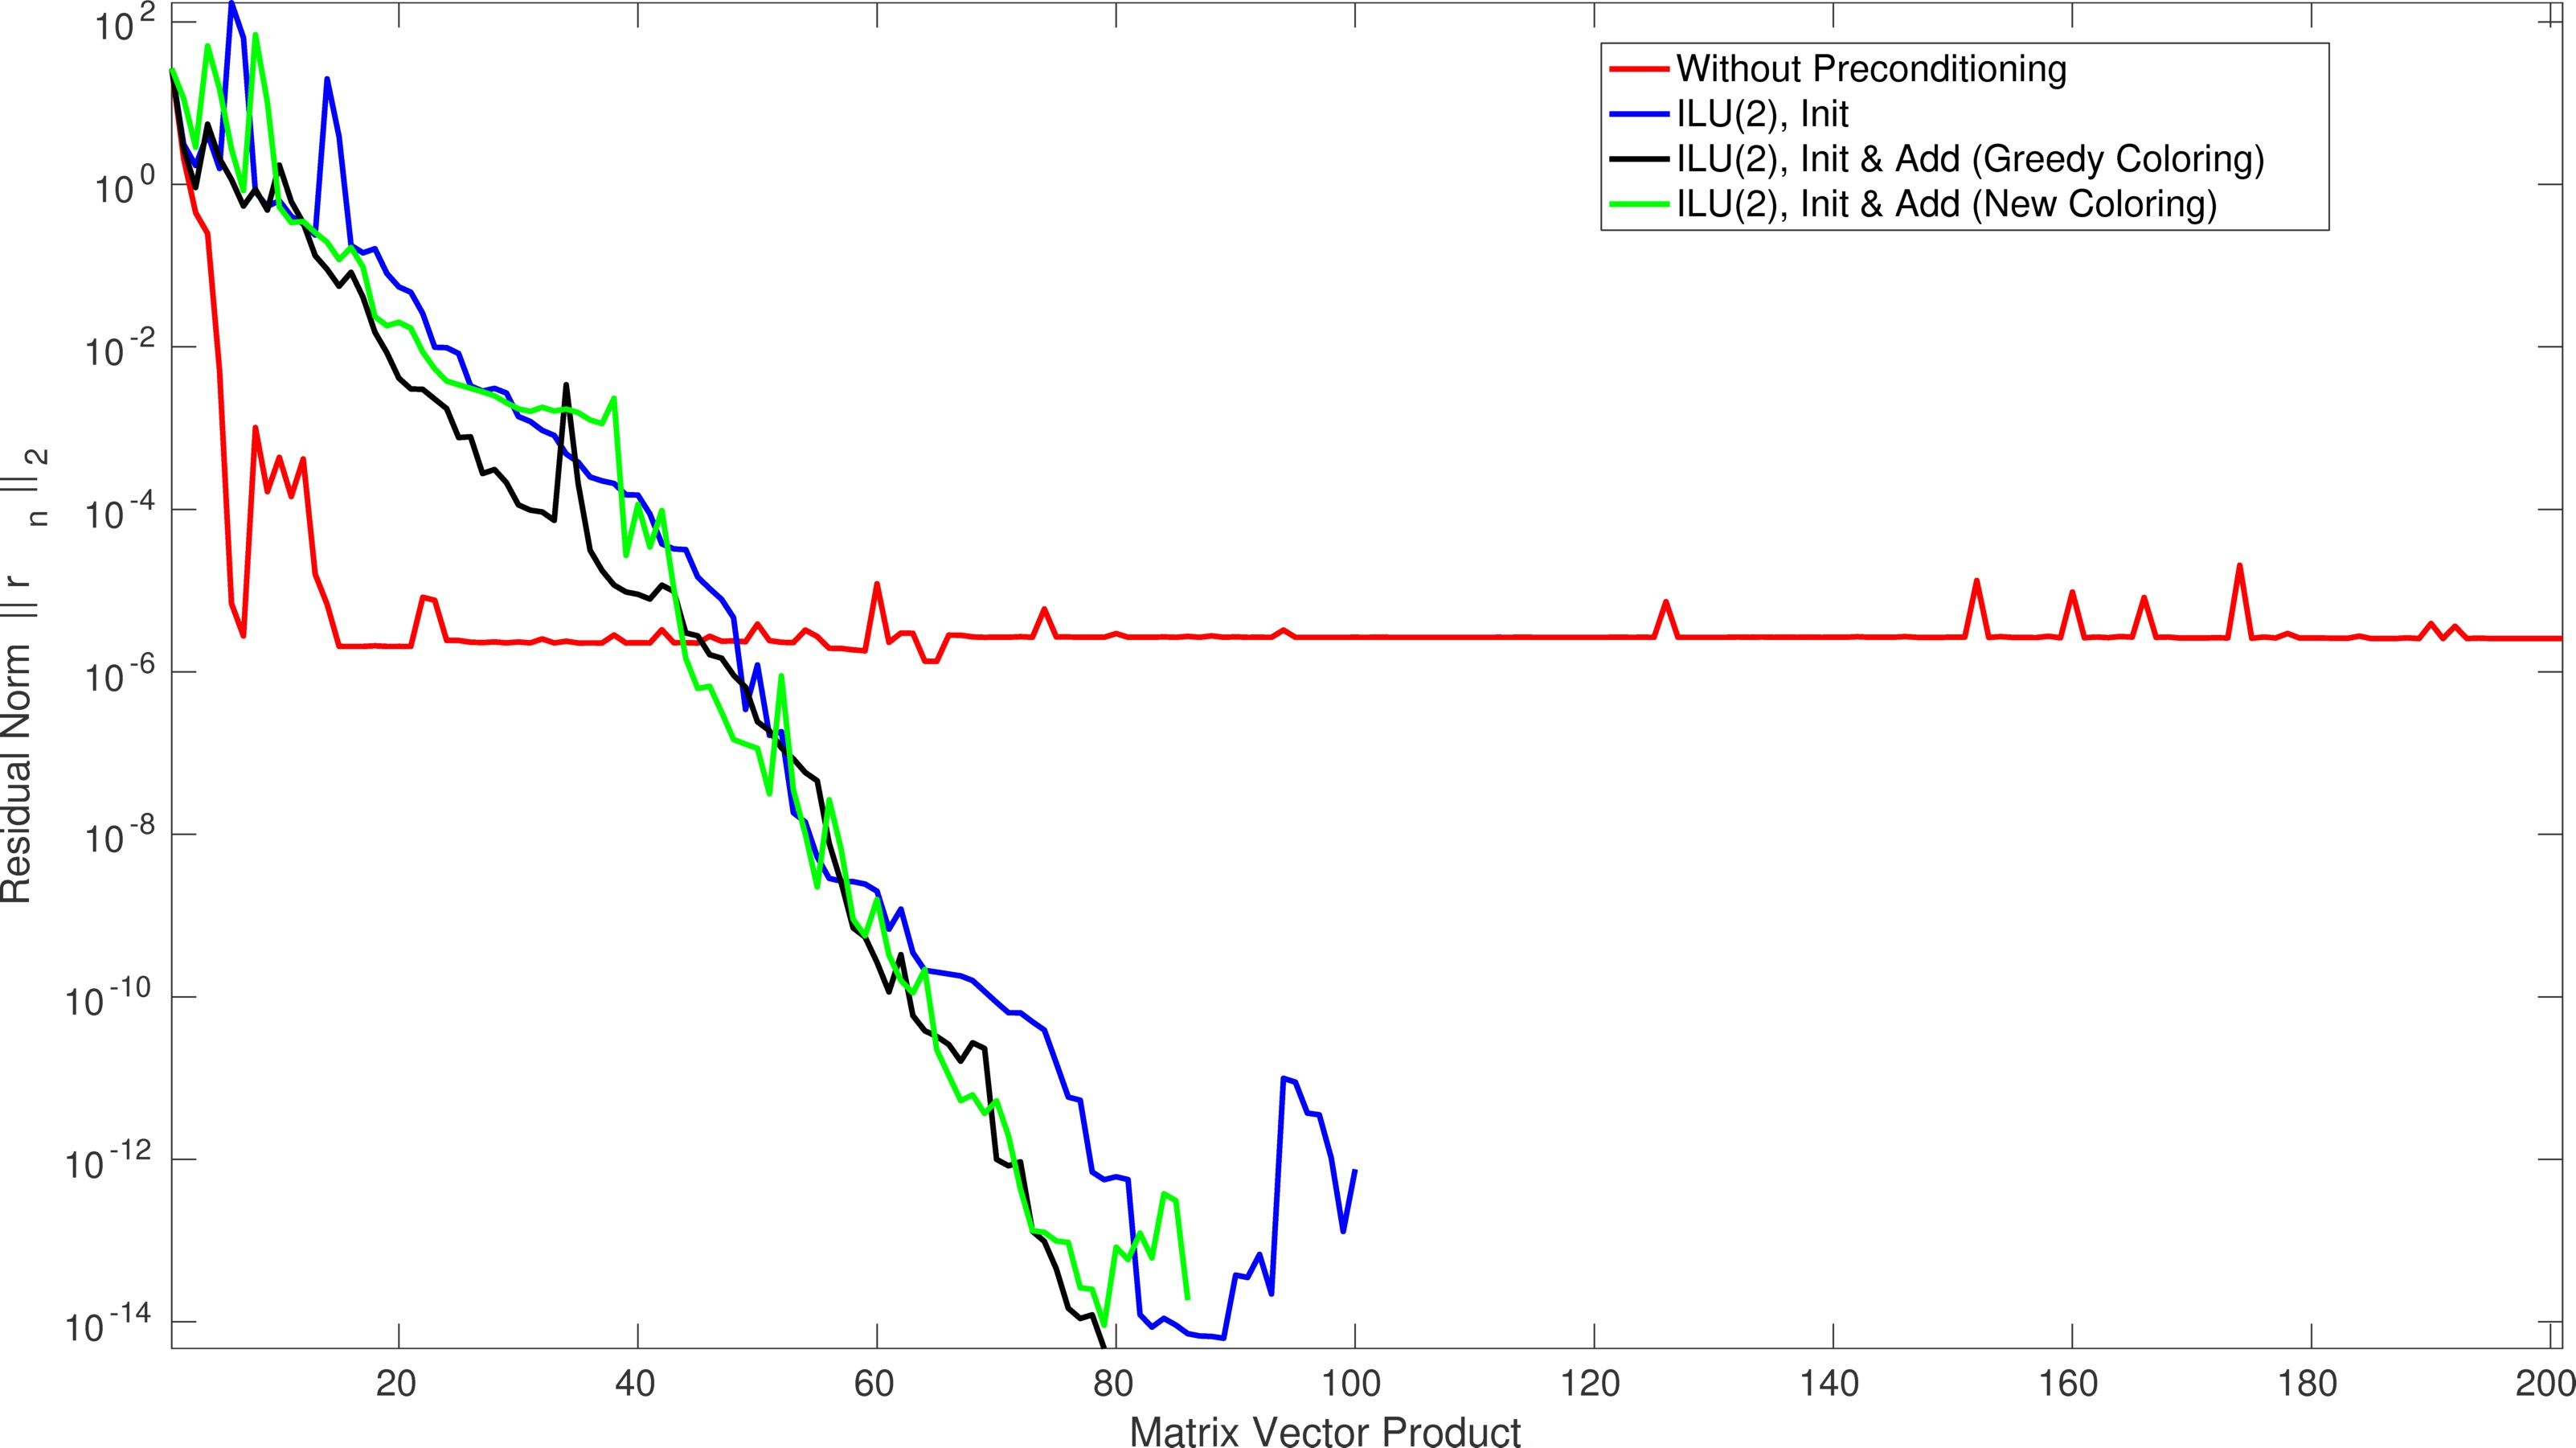
\includegraphics[width=0.8\linewidth]{jac_convergence_greedy_new_bl2.jpg}
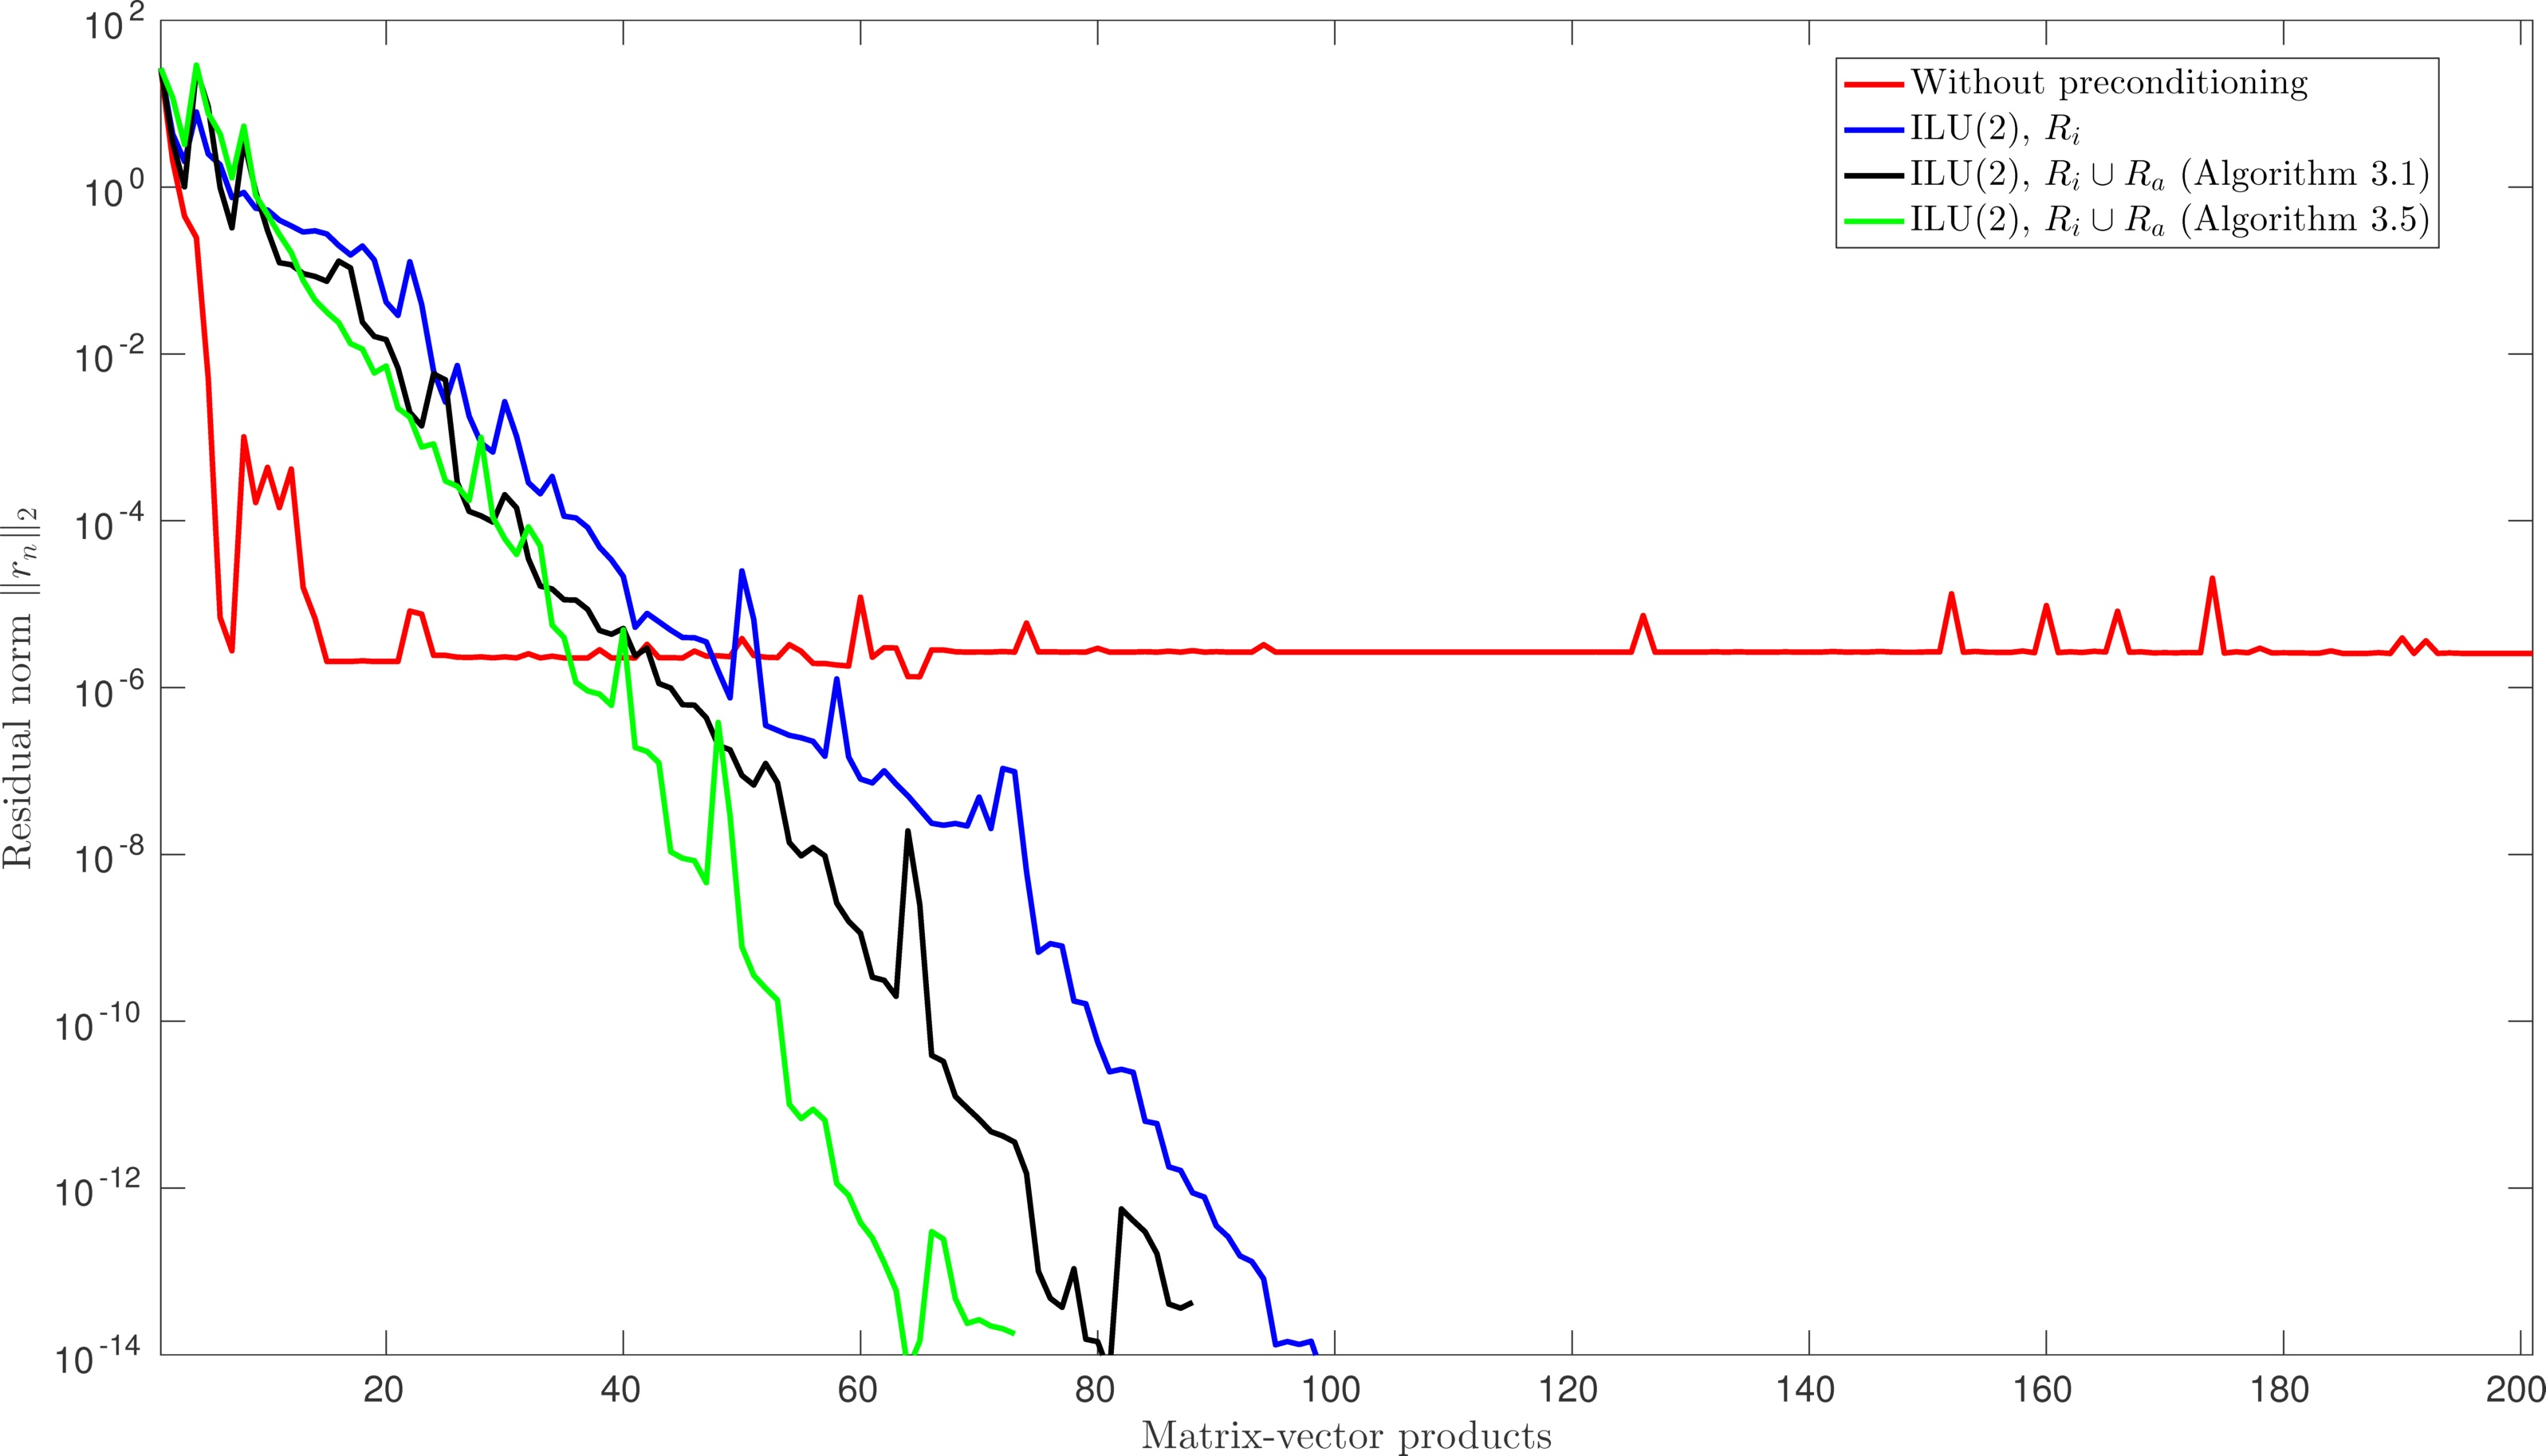
\includegraphics[width=\linewidth]{jac_convergence_greedy_new_5.jpg}
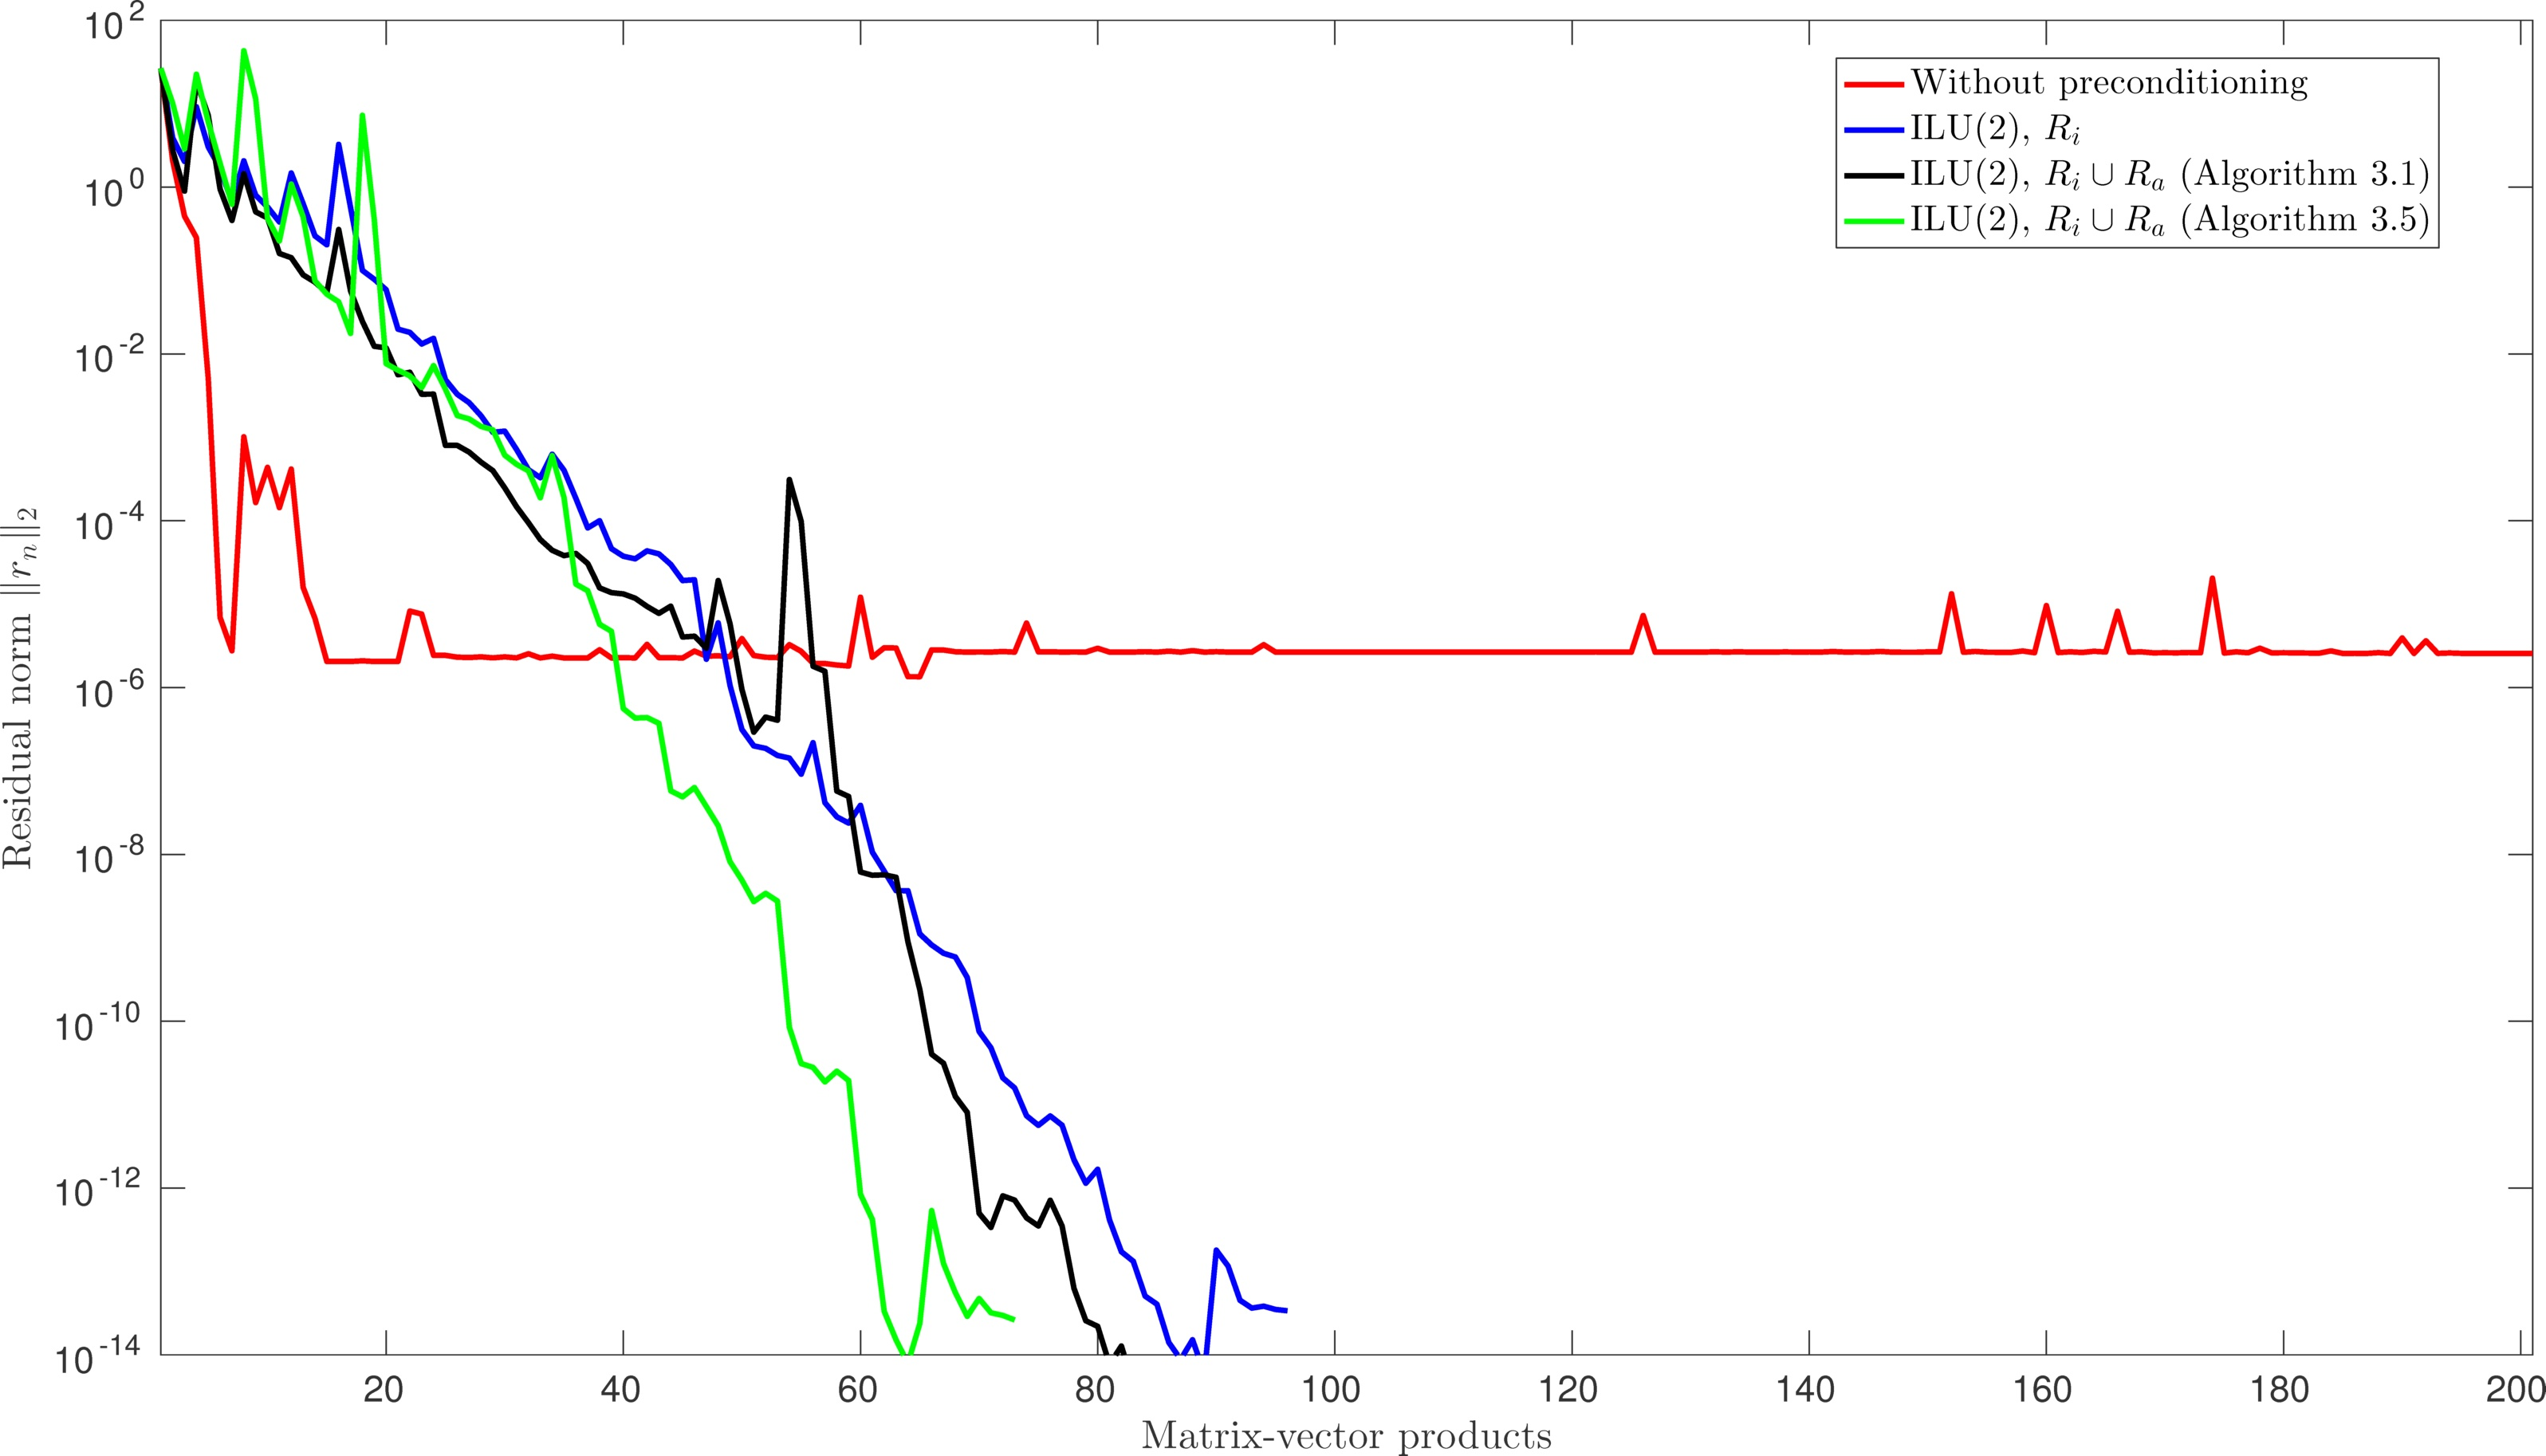
\includegraphics[width=\linewidth]{jac_convergence_greedy_new_10.jpg}
\caption{
The history of the residual norms is visualized based on
the number of matrix-vector products comparing four different methods:
without preconditioning (red color),
preconditioning with $S=R_i$ (blue color),
preconditioning with $S=R_i + R_a$ in which
the set $R_a$ is computed based on the greedy coloring (black color),
and preconditioning with $S=R_i + R_a$ in which
the set $R_a$ is computed based on \coderef{code.new.impr2} (green color).
The level parameter of the ILU preconditioning is $2$.
(Top) The block size is $5$.
(Bottom) The block size is $10$.
}
\label{f.convergence_greedy_new2}
\end{figure}

\begin{figure}
\centering
%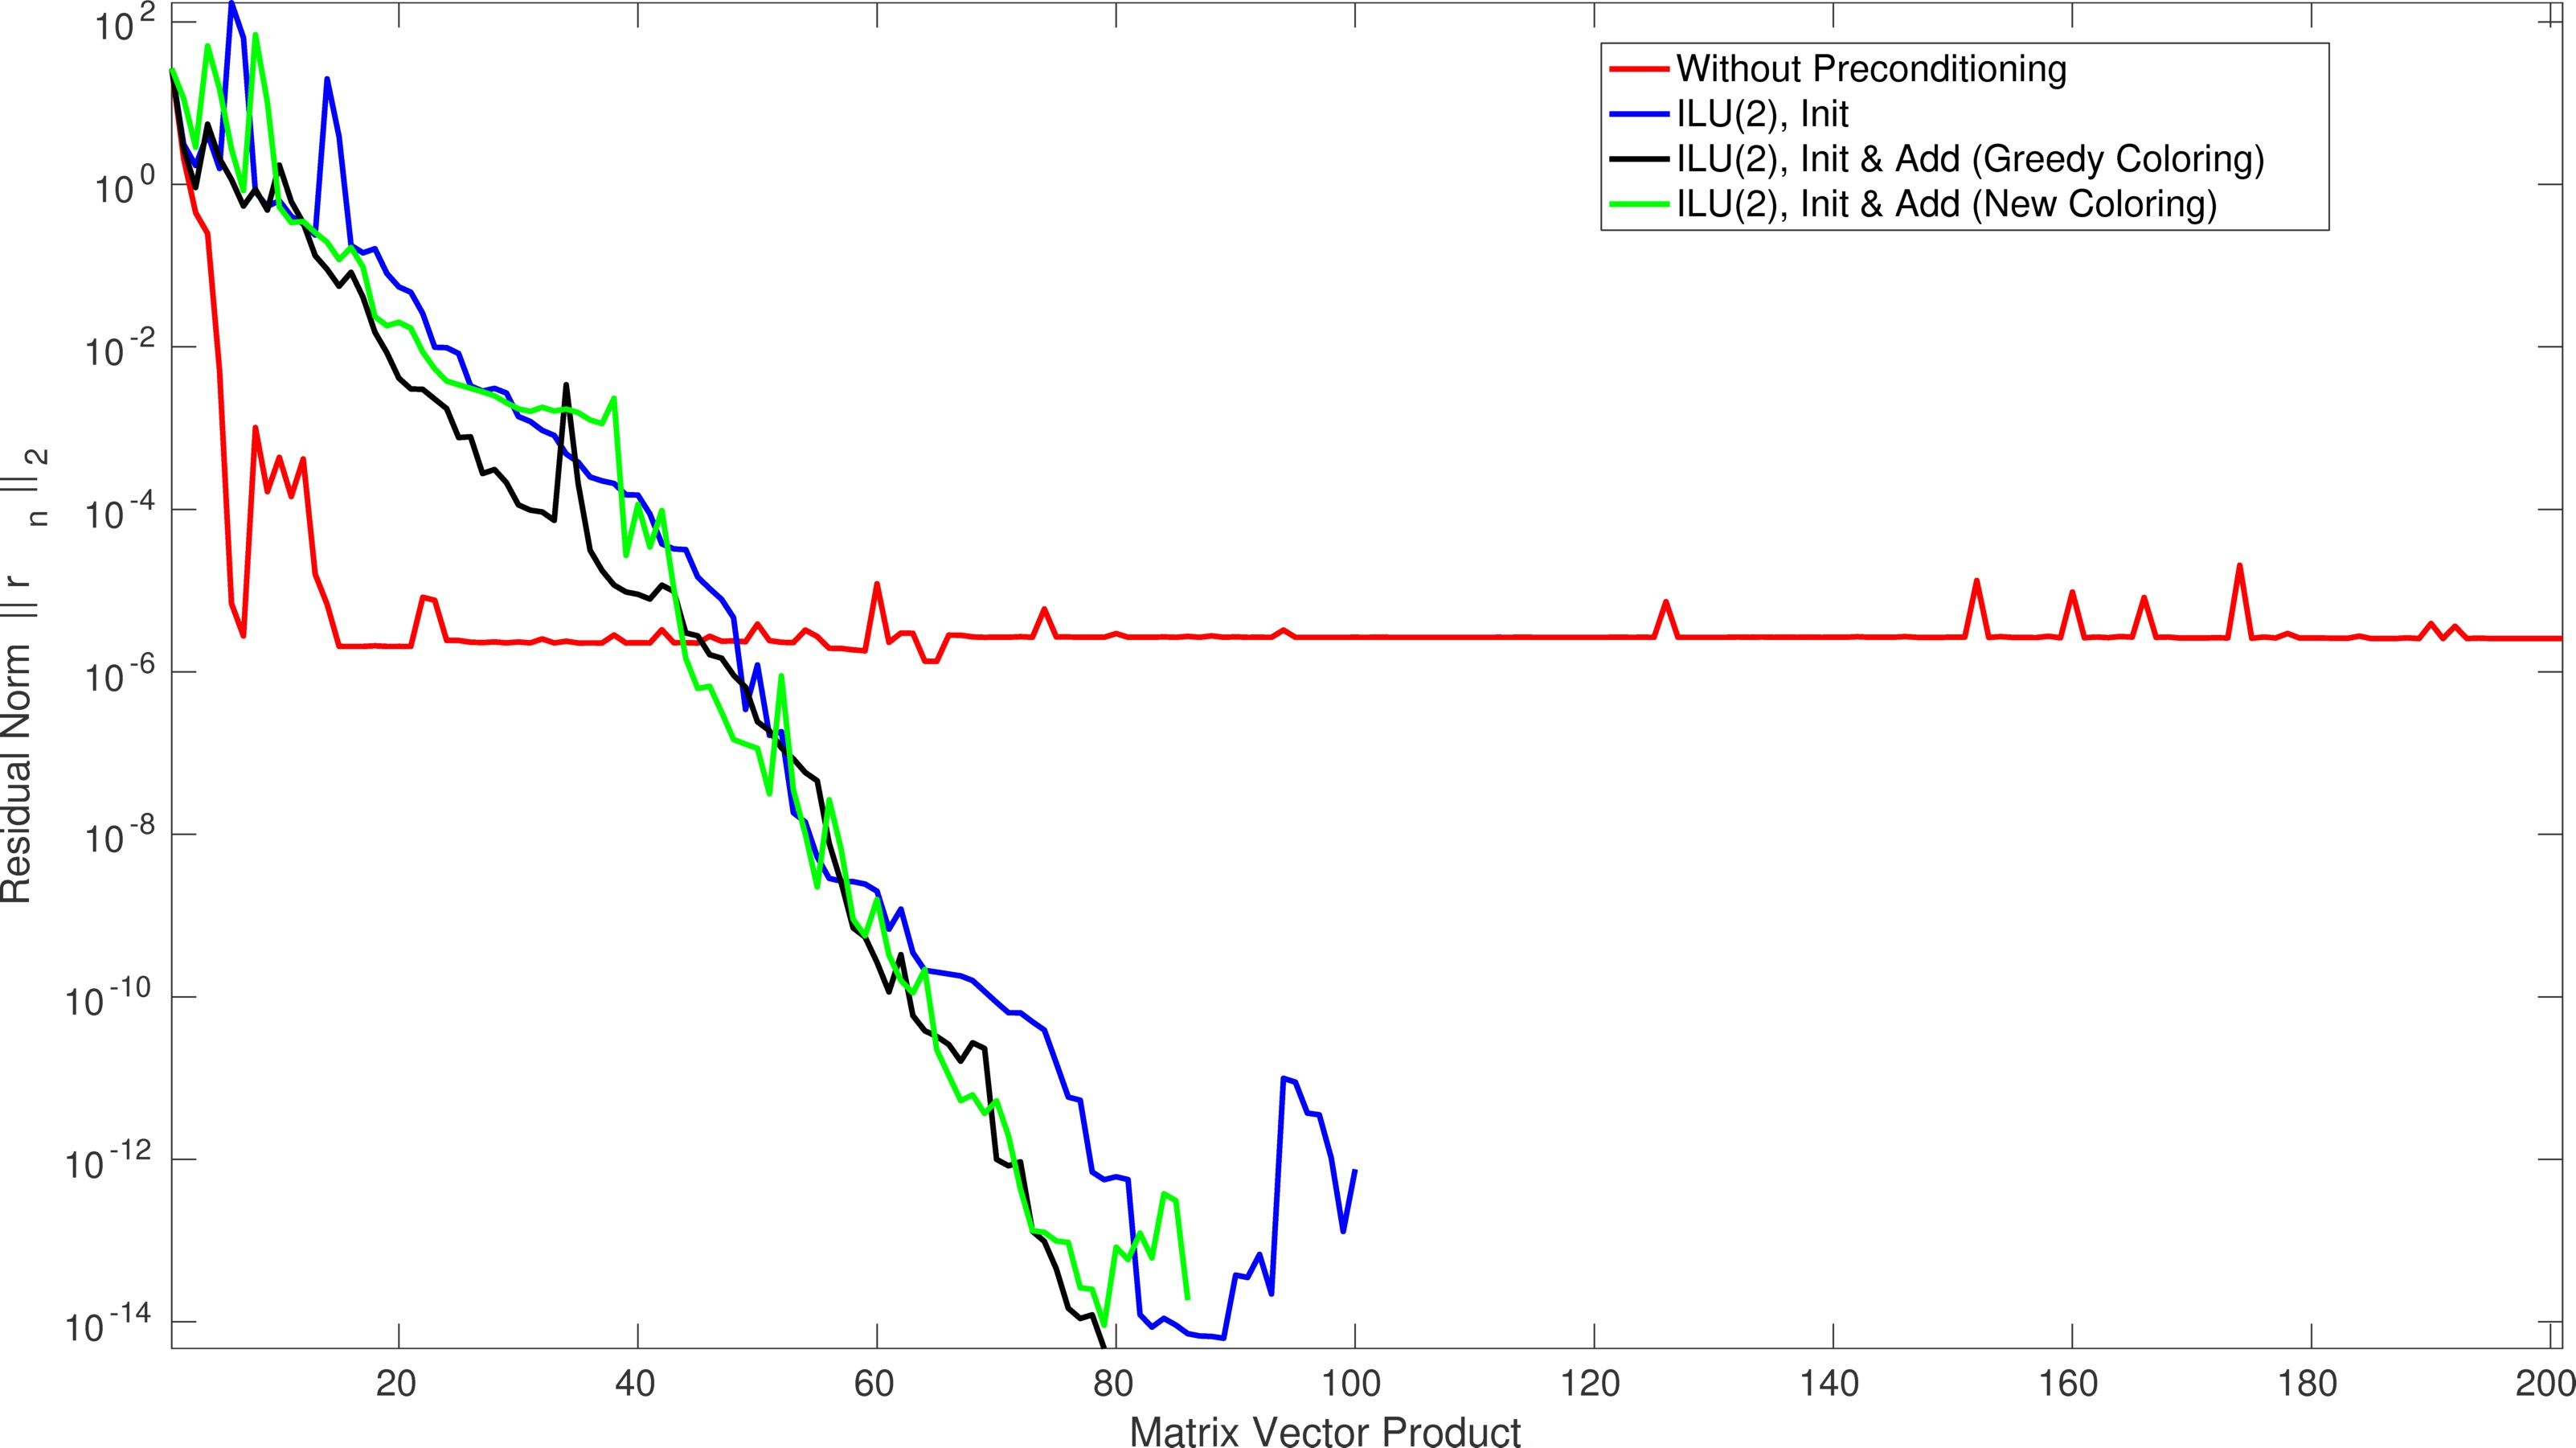
\includegraphics[width=0.8\linewidth]{jac_convergence_greedy_new_bl2.jpg}
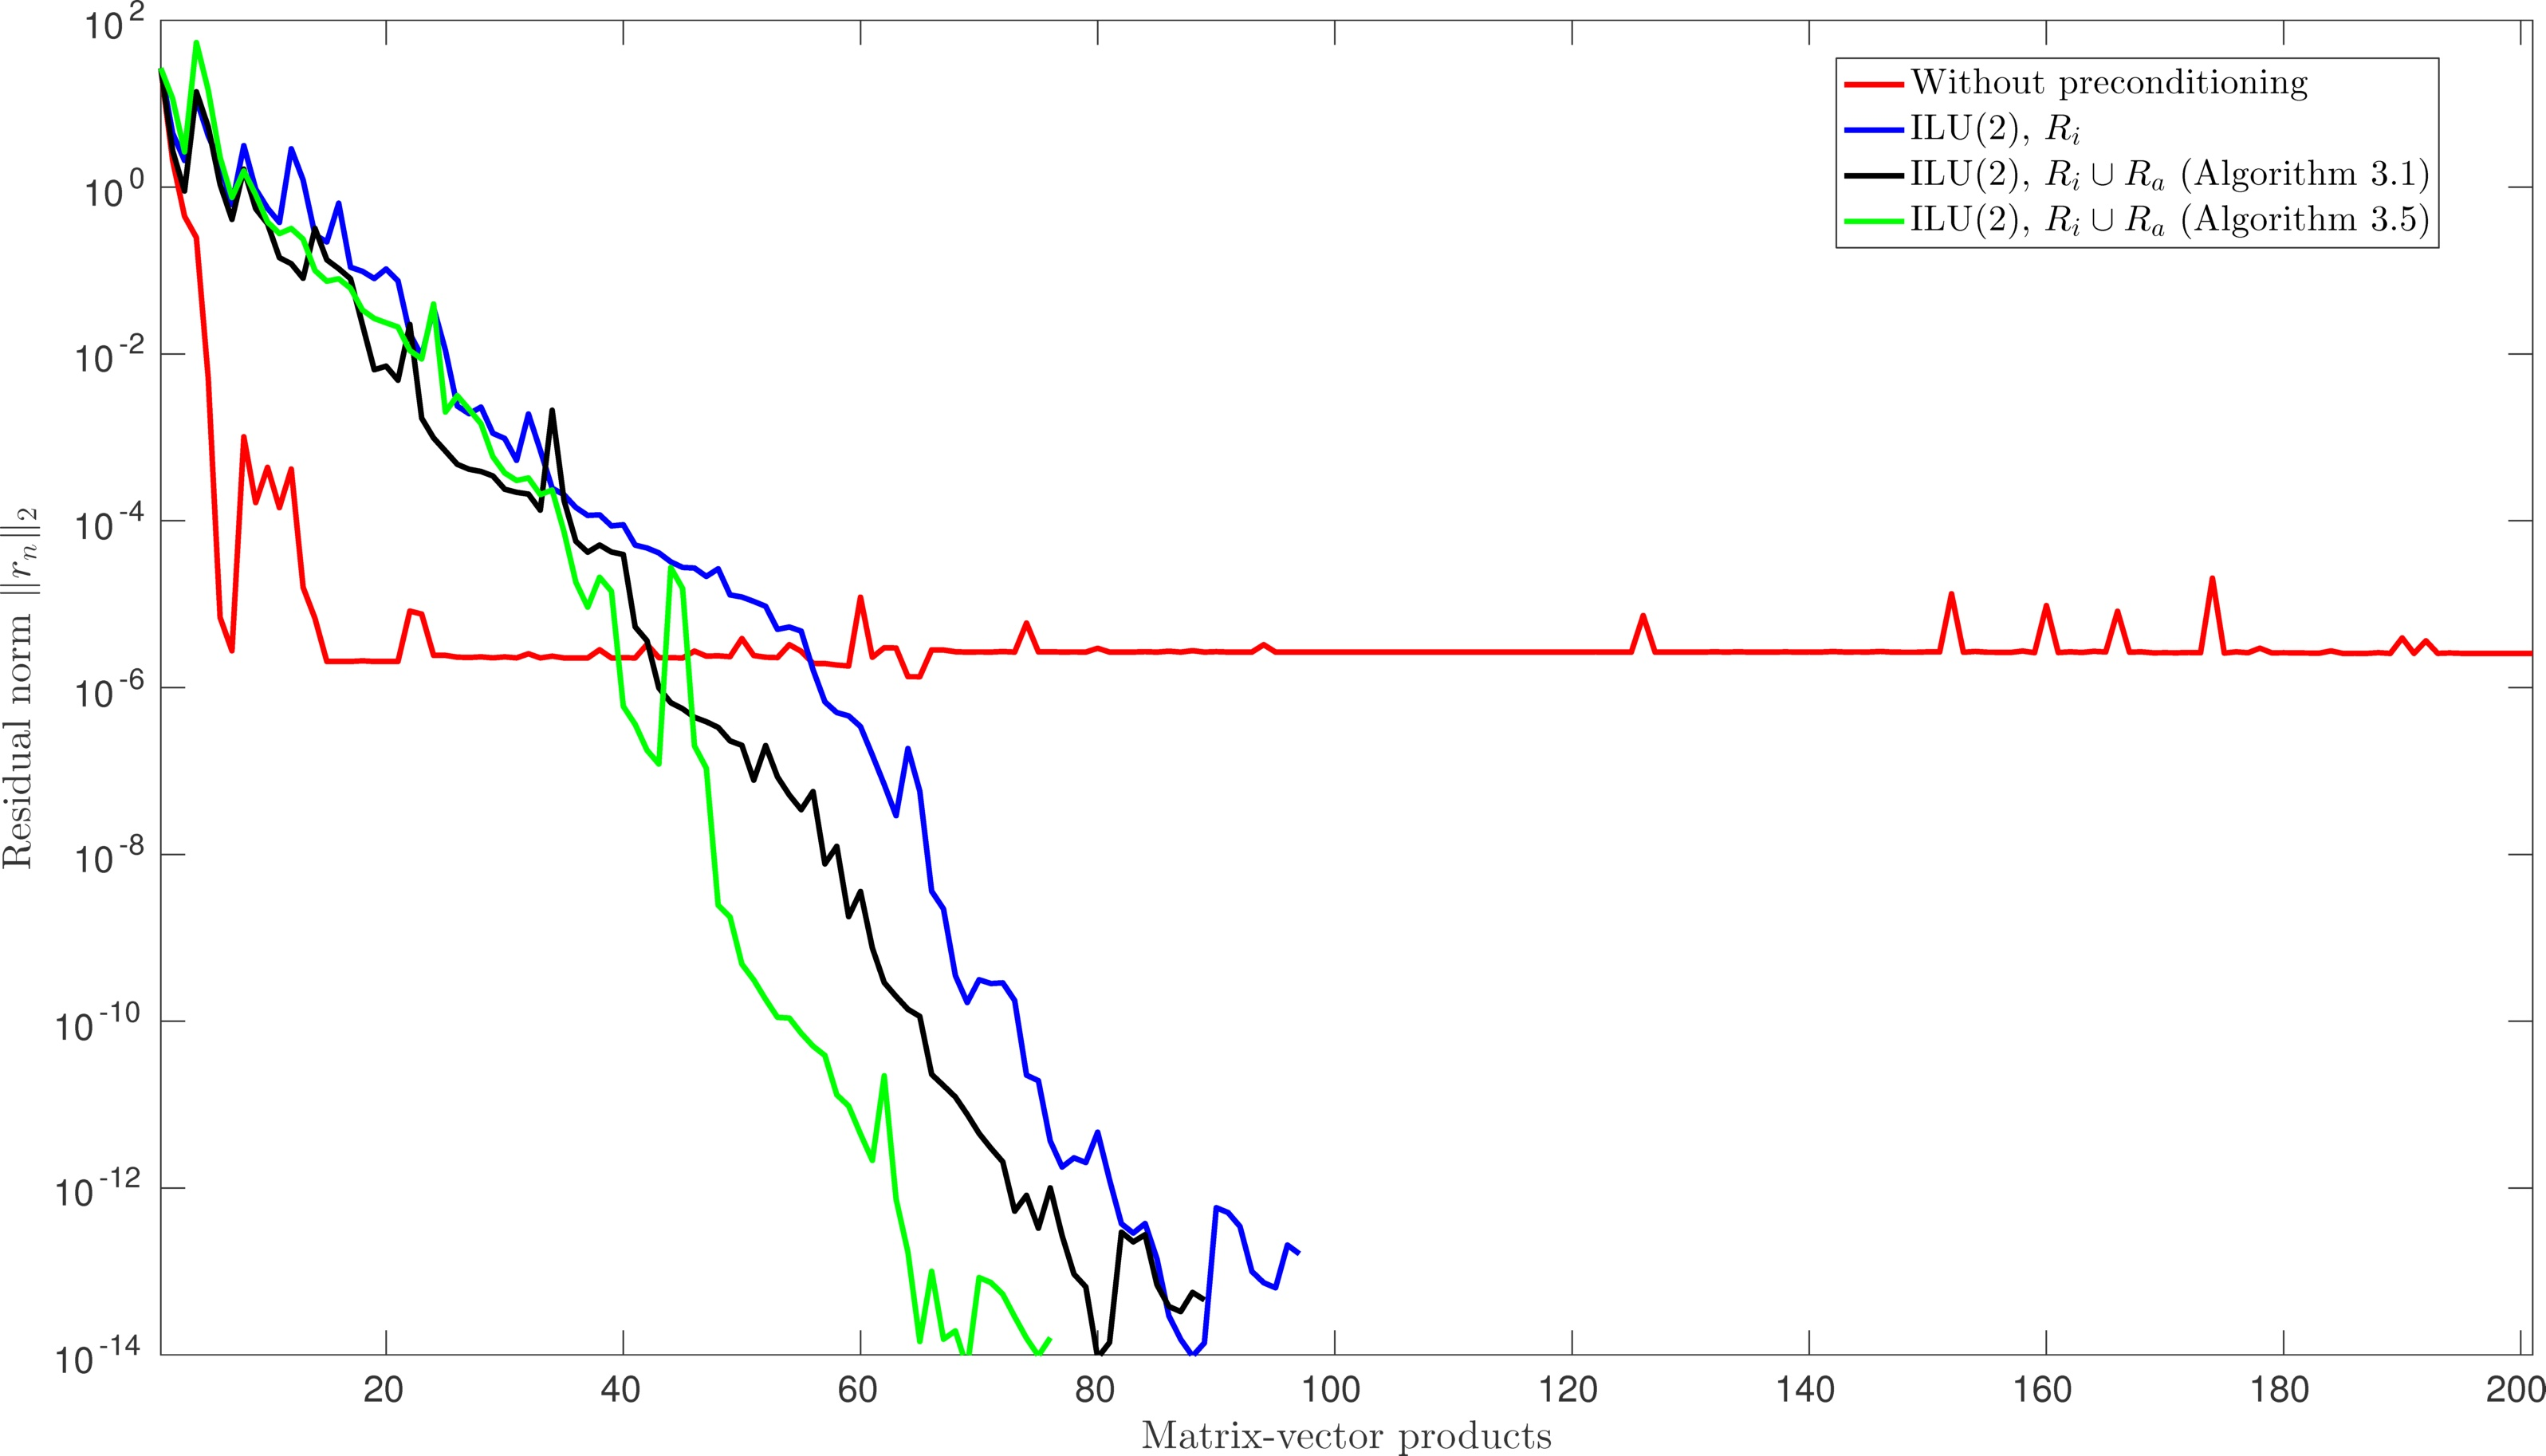
\includegraphics[width=\linewidth]{jac_convergence_greedy_new_15.jpg}
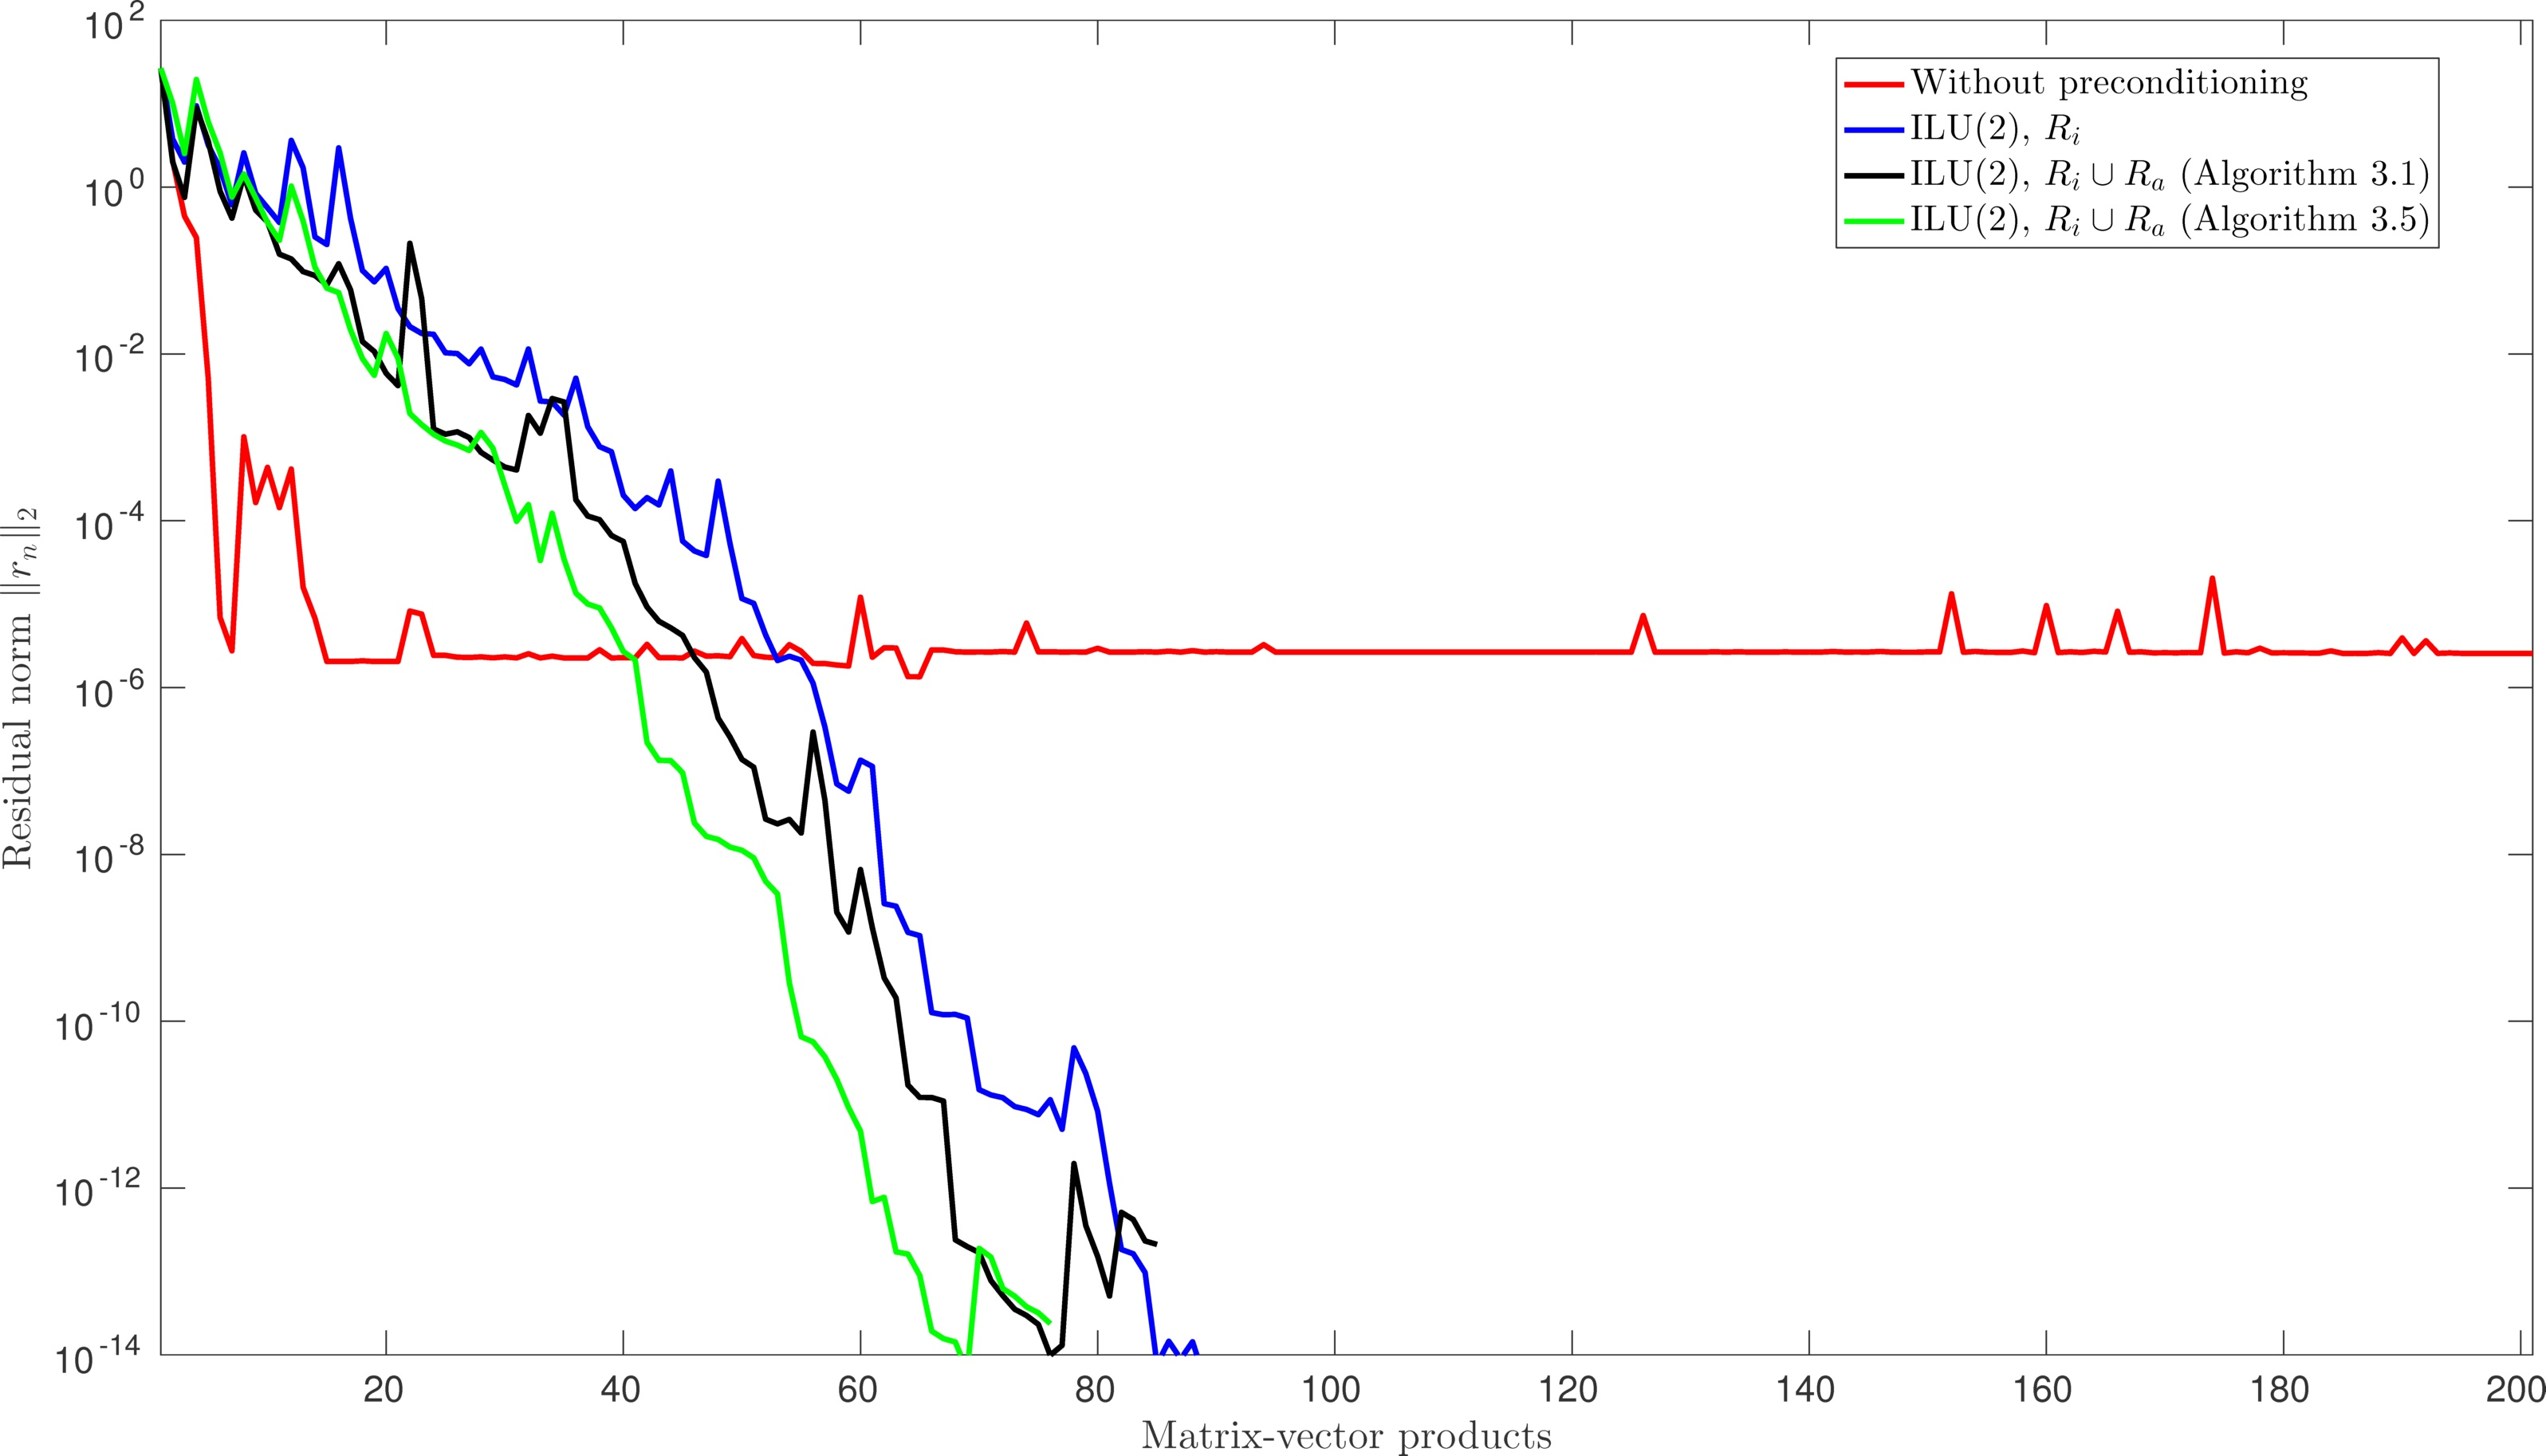
\includegraphics[width=\linewidth]{jac_convergence_greedy_new_20.jpg}
\caption{
The history of the residual norms is visualized based on
the number of matrix-vector products comparing four different methods:
without preconditioning (red color),
preconditioning with $S=R_i$ (blue color),
preconditioning with $S=R_i + R_a$ in which
the set $R_a$ is computed based on the greedy coloring (black color),
and preconditioning with $S=R_i + R_a$ in which
the set $R_a$ is computed based on \coderef{code.new.impr2} (green color).
The level parameter of the ILU preconditioning is $2$.
(Top) The block size is $15$.
(Bottom) The block size is $20$.
}
\label{f.convergence_greedy_new3}
\end{figure}

\begin{table}
\centering
\begin{tabular}{|c|c|c|c|c|c|c|}
\hline
Size & \multicolumn{3}{c|}{\coderef{code.greedy}} & \multicolumn{3}{c|}{\coderef{code.new.impr2}}\\\hline
{} & $|R_p|$ & $|R_a|$ & $|\Phi|$ & $|R_p|$ & $|R_a|$ & $|\Phi|$\\\hline
$1$ & $734$ & $724$ & $6$ & $1212$ & $786$ & $7$\\\hline
$2$ & $1670$ & $886$ & $11$ & $1730$ & $990$ & $10$\\\hline
$3$ & $1316$ & $776$ & $10$ & $1952$ & $1052$ & $14$\\\hline
$4$ & $1838$ & $1016$ & $13$ & $1952$ & $1070$ & $14$\\\hline
$5$ & $1524$ & $896$ & $13$ & $1976$ & $1070$ & $15$\\\hline
$6$ & $1456$ & $732$ & $13$ & $1828$ & $974$ & $13$\\\hline
$7$ & $1596$ & $852$ & $11$ & $1770$ & $942$ & $13$\\\hline
$8$ & $1758$ & $928$ & $13$ & $1880$ & $976$ & $13$\\\hline
$9$ & $1750$ & $912$ & $13$ & $1826$ & $966$ & $13$\\\hline
$10$ & $1704$ & $960$ & $13$ & $1826$ & $992$ & $13$\\\hline
$11$ & $1744$ & $904$ & $13$ & $1832$ & $940$ & $13$\\\hline
$12$ & $1738$ & $900$ & $13$ & $1760$ & $938$ & $13$\\\hline
$13$ & $1712$ & $874$ & $13$ & $1918$ & $1022$ & $13$\\\hline
$14$ & $1572$ & $782$ & $13$ & $1572$ & $848$ & $13$\\\hline
$15$ & $1728$ & $914$ & $13$ & $1836$ & $928$ & $13$\\\hline
$16$ & $1704$ & $870$ & $13$ & $1842$ & $956$ & $13$\\\hline
$17$ & $1702$ & $866$ & $13$ & $1812$ & $940$ & $14$\\\hline
$18$ & $1696$ & $858$ & $13$ & $1704$ & $874$ & $13$\\\hline
$19$ & $1694$ & $860$ & $13$ & $1784$ & $940$ & $13$\\\hline
$20$ & $1688$ & $854$ & $13$ & $1810$ & $956$ & $13$\\\hline
\end{tabular}
\caption{The comparison between the number of potentially and additionally required
elements and the number of colors computed with \coderef{code.greedy} and \coderef{code.new.impr2}.
The computation is carried out on the matrix $A$.
The block size is from $1$ to $20$. The ordering is the natural ordering.}
\label{bls.greedy.new.carbon}
\end{table}

\clearpage
%%%%%%%%%%%%%%%%%%%%%%%%%%%%%%%%%%%%%%%%%%%%%%%%%%%%%%%%%%%%%%%%%%%%%%%%%%%%%%%%%%%%%%%%%%%%%%
\section{Coloring restricted to diagonal elements}
\label{s.part.color.diag}
%%%%%%%%%%%%%%%%%%%%%%%%%%%%%%%%%%%%%%%%%%%%%%%%%%%%%%%%%%%%%%%%%%%%%%%%%%%%%%%%%%%%%%%%%%%%%%
Here, we look at a particular example in which the sparsity pattern is restricted to diagonal elements.
Lülfesmann~\cite{Lulfesmann2012Fap} shows that the minimum number of colors of
the star bicoloring restricted to diagonal elements $\chi_{sb}$ is equal to
the minimal number of colors of the distance-$2$ coloring restricted
to diagonal elements $\chi_{d2}$.
It means that the bidirectional compression restricting to diagonals is not better than
a distance-$2$ coloring restricted to diagonal elements.
This theorem can be written as two lemmas,
\begin{itemize}
\item Lemma 1: $\chi_{sb} \geq \chi_{d2}$
\item Lemma 2: $\chi_{sb} \leq \chi_{d2}$
\end{itemize}
The proof of Lemma 2 is clear since
a given distance-$2$ coloring with the fewest number of colors is also a star bicoloring.
The proof of Lemma 1 is more tricky. A sketch of the proof is as follow.
\begin{figure}
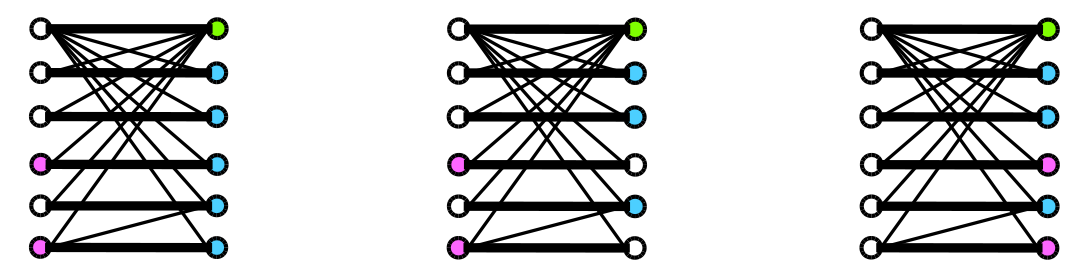
\includegraphics[width=\linewidth]{proof1.png}
\caption{
(Right) An example of a star bicoloring restricted to diagonal elements
transformed to a valid distance-$2$ coloring.}
\label{proof1}
\end{figure}


The idea is to transform a valid star bicoloring with the fewest number of colors $\Phi_{sb}$ to
a valid distance-$2$ coloring where the number of colors is not larger.
This transformation includes two steps:
\begin{enumerate}
\item The minimal star bicoloring $\Phi_{sb}$ is transformed
to the valid star bicoloring $\Phi_{sb}^{*}$
where exactly one of both incident vertices of each required edge is colored nonzero.
\item The valid coloring $\Phi_{sb}^{*}$ is transformed
to the valid star bicoloring $\Phi_{sb}^{'}$ where all row vertices are colored by zero.
This star bicoloring is also a distance-$2$ coloring.
\end{enumerate}
An example of this transformation can be seen in \figref{proof1}.
Looking at the proof of Lemma 3.8 of Lülfesmann~\cite{Lulfesmann2012Fap}, this lemma (and consequently Theorem 3.10 of Lülfesmann~\cite{Lulfesmann2012Fap})
can be generalized by considering any coloring instead of the optimal coloring.
Also, the set of diagonal elements in the theorem
can be replaced by any set of required elements
in which each column and row contain only one required nonzero element.
This property is nothing but a matching~\cite{bondy2008graph} in a graph.
Given a graph and the vertex and edge set $G=(V,E)$, a matching $M\subseteq E$ contains
a list of edges which do not have any vertex in common.
A maximum matching is a matching with a maximum possible number of edges.
Then, all diagonal elements for example in our bipartite graph is a maximum matching.

Now, we can formulate a new theorem on the comparison of unidirectional and
bidirectional coloring as follows.
\begin{theorem}
\label{t.matching}
Given the bipartite graph $G=(V_r\cup V_c,E)$ and a matching $M\subseteq E$ representing
the required elements, any valid star bicoloring restricted to $M$
with the number of colors $X_{sb}$
can be transformed to a valid distance-$2$ coloring restricted to $M$
with the number of colors $X_{d2}$ such that $X_{sb} \geq X_{d2}$.
These numbers of colors can be different from the minimal number of colors.
\end{theorem}
This theorem is a generalization of Lemma 3.8 of \cite{Lulfesmann2012Fap}.
This lemma discusses only the mapping with minimal coloring
and the coloring restricted to diagonal elements. We consider any coloring
restricted to a matching.
The proof for that lemma can be applied to this new theorem considering the two following points,
\begin{itemize}
\item The minimality of colorings is only used to show the equality in the number of colors which is not
the case in our theorem.
\item The property of being diagonal elements is used in the proof from \cite{Lulfesmann2012Fap} only to
make the required edges disjoint from each other which is the definition of a matching in a graph.
\end{itemize}

This generalization gives us an idea to find new heuristics for coloring in which
we color the column and row vertices simultaneously.
The motivation of this new heuristic is from the following observation.
Next we compare the number of colors computed by \coderef{code.greedy} and \coderef{orig.star.bicoloring}
in Table~\ref{table.starbic.d2.diag} for different matrices.
The better results are observed in \coderef{orig.star.bicoloring} for some matrices.
These examples also show that the inequality in Theorem~\ref{t.matching} can happen.
The second column of this table
shows the number of colors computed by \coderef{orig.star.bicoloring}.
The third column shows the minimum number of colors computed by the greedy coloring in~\coderef{code.greedy}
either for rows or columns.
It can be seen that even for a small matrix as the matrix \textit{cage3} which has only
$5$ rows and columns, the star bicoloring can produce a better result.

\begin{table}
\centering
\begin{tabular}{|c|c|c|}
\hline
Matrix & $\Phi_{sb}$ & min($\Phi_r$,$\Phi_c$)\\\hline
\textit{cage3} & $3$ & $4$\\\hline
\textit{cage4} & $3$ & $4$ \\\hline
\textit{cage5} & $5$ & $7$\\\hline
\textit{cage7} & $7$  & $8$\\\hline
\textit{cage8} & $8$  & $10$\\\hline
\textit{cage9} & $9$  & $11$\\\hline
\textit{cage10} & $10$ & $11$\\\hline
\textit{cage12} & $13$ &  $14$\\\hline
\end{tabular}
\hfill
\begin{tabular}{|c|c|c|}
\hline
Matrix & $\Phi_{sb}$ & $\min(\Phi_r,\Phi_c)$\\\hline
\textit{ex7} & $18$ & $22$ \\\hline
\textit{nos3} & $10$ & $10$ \\\hline
\textit{steam1} & $6$ & $6$ \\\hline
\textit{steam2} & $8$ & $8$ \\\hline
\textit{rajat01} & $8$ & $8$ \\\hline
\textit{gyro\_m} & $15$ & $15$\\\hline
\textit{ex33} & $12$ & $11$\\\hline
\textit{cavity16} & $20$ & $18$ \\\hline
\end{tabular}

\caption{The comparison of the number of colors in star bicoloring restricted to diagonals $\Phi_{sb}$
computed by \coderef{orig.star.bicoloring}
and in distance-$2$ coloring restricted to diagonals $\min(\Phi_r,\Phi_c)$ (either for rows or for columns) 
computed by \coderef{code.greedy}.
The ordering is the natural ordering of the matrix for both colorings.}
\label{table.starbic.d2.diag}
\end{table}

More clearly, the idea is that a heuristic for star bicoloring maybe
finds a better coloring than a distance-$2$ coloring because of the inequality in the theorem.
As the proof of the theorem proposes, every required nonzero element
can be determined by either a column or a row, but not both.
\coderef{star.diagonal} shows our new heuristic. This heuristic
iterates over the required edges.
In each iteration, we simultaneously execute a distance-$2$ coloring for both
incident vertices of the required edge. This greedy approach finds the minimum possible colors $c_1$ for columns
and $c_2$ for rows, each in a separate fashion.
Then, the recombination of these two separate distance-$2$ colorings into a star bicoloring is given by coloring the vertex with the corresponding smaller color.
In numerical experiments we observe that the number of colors computed by this new heuristic is equal to $\Phi_{sb}$
for the matrices from Table~\ref{table.starbic.d2.diag}.

\begin{figure}
\begin{lstlisting}[
caption=An improved star bicoloring restricted to diagonal elements.
As the theorem says this coloring generates an equivalent distance-$2$ coloring.,
label=star.diagonal,mathescape]
function star_diag($G=(V_r\cup V_c, E)$, $E_i\subseteq E$)
  $\Phi\leftarrow [0\ldots 0]$
  $forbiddenColors1\leftarrow [0\ldots 0]$
  $forbiddenColors2\leftarrow [0\ldots 0]$

  for $e=(v,u)\in E_i$ with $v \in V_c$ and $u \in V_r$
    $forbiddenColors1[0] = v$
    $forbiddenColors2[0] = u$

    for $n\in N_2(v,E_i)$ with $\Phi(n)\neq 0$
        $forbiddenColors1[\Phi(n)] = v$

    for $n\in N_2(u,E_i)$ with $\Phi(n)\neq 0$
        $forbiddenColors2[\Phi(n)] = u$

    $c_1 = \min(\{j>0: forbiddenColors1[j] \neq v\})$
    $c_2 = \min(\{j>0: forbiddenColors2[j] \neq u\})$

    if $c_1 < c_2$
      $\Phi(v) = c_1$
    else
      $\Phi(u) = c_2$

  return $\Phi$
\end{lstlisting}
\end{figure}


%%%%%%%%%%%%%%%%%%%%%%%%%%%%%%%%%%%%%%%%%%%%%%%%%%%%%%%%%%%%%%%%%%%%%%%%%%%%%
\clearpage
\section{Implementation details of PreCol}
\label{s.extend}
%%%%%%%%%%%%%%%%%%%%%%%%%%%%%%%%%%%%%%%%%%%%%%%%%%%%%%%%%%%%%%%%%%%%%%%%%%%%%
We develop a piece of software to implement our proposed heuristics.
Specifically, the software is designed employing concepts from object-oriented programming
such that it can be extended further with new coloring heuristics as well as preconditioning algorithms.
The developers can implement new extensions without going into the details of the core implementation.
Two main ingredients, coloring and orderings, can be implemented only by deriving an interface.
For example, a new coloring and ordering can be added as easy as the following code.
\begin{lstlisting}
class New_Ordering : public Ordering {
  void order(const Graph &G, vector<unsigned int> &ord, bool restricted) {...}
};

class New_Coloring : public ColAlg {
   vector<int> color() {...}
};
\end{lstlisting}
Here, the computed ordering is saved in the array \textit{ord} and the coloring is the output
of the function \textit{color}.

The developer needs to implement these new classes in an only-header fashion~\cite{headeronly}
since the goal is to write an extension with little effort. So, the developer should
move the new header file to the corresponding directory which is the \textit{ordering} directory
for this new ordering and the \textit{algs} directory for coloring algorithms.
Now, building the software will bring this new ordering into the software execution.

The input matrix is in the format of the matrix market~\cite{matrix-market}.
After reading this matrix, we convert it to the different graph models
like a column-intersection graph or a bipartite graph.
Any resulting matrix like the sparsified matrix will also be saved in this file format.

\textit{PreCol} is developed in \textit{C++} using STL (the standard library) and
the boost library~\cite{boost}.
Using concepts of functional programming
in the new C++ release (C++11 and C++14)~\cite{Sutherland2015},
we provide different functions which can be used
by a developer to work on graphs. For example, the iteration on vertices
or edges can be as easy as follows.
\begin{lstlisting}
for_each_v(G, f);
for_each_v(G, [&](Ver v) {...});
for_each_e(G, f);
for_each_e(G, [&](Edge e) {...});
\end{lstlisting}
in which the variable $f$ is a function which gets an input parameter of a vertex or an edge.
Also, the other syntax is the lambda function
from the new C++ functional programming to implement an unnamed function.

Following a unique solution, we implement all parts of our heuristics
with the use of the standard library of \textit{C++} which also improves the readability.
This strategy reduces the code length dramatically.
Also, the algorithms of the \textit{C++} standard library will automatically be parallel in \textit{C++17}~\cite{parallelcpp}.

As it is presented in \figref{f.structure}, the computations of coloring and ILU preconditioning
are in one package available in \textit{C++}. But, the computation of iterative solvers is carried out
in MATLAB.
%-----------------------------------------------------------------------------------------------
\begin{figure}
\centering
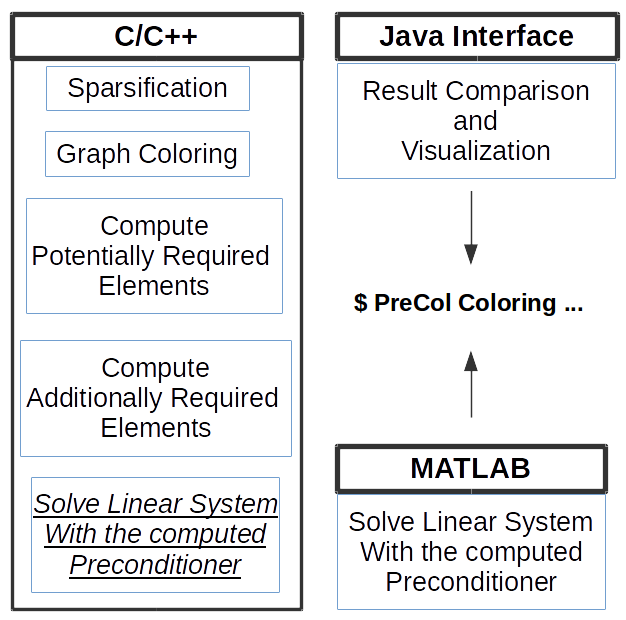
\includegraphics[width=0.52\textwidth]{new_struct}
\caption{
The software \textit{PreCol} and two user interfaces written in MATLAB and Java.}
\label{f.structure}
\end{figure}
%-----------------------------------------------------------------------------------------------

To use the software, the user can use a shell command.
So, the user needs to specify different
options for coloring algorithms, orderings, the block size, and so on.
These options can be entered directly in the terminal.
An example is as follows.
\begin{lstlisting}
precol PartialD2RestrictedColumns LFO_Nat BlockDiagonal 30 2 ex33.mtx
\end{lstlisting}
in which the \textit{PartialD2RestrictedColumns} is the coloring algorithm,
the string \textit{LFO\_Nat} containing
two strings \textit{LFO} and \textit{Nat} are for the coloring and ILU orderings.
The next parameter \textit{BlockDiagonal} specifies the sparsification method
which is followed by the size of the block. Here, the block size is $30$.
The next number $2$ specifies the level parameter of ILU.
The matrix name is the last parameter.

We develop two user interfaces for \textit{PreCol}.
So that it can be called from within MATLAB and GraphTea~\cite{2014:07,2014:15}.
These user interfaces help to evaluate our proposed heuristics.
Both interfaces execute the binaries of \textit{PreCol}
and process the output files generated by \textit{PreCol}.
The corresponding commands in both interfaces can be executed by the following parameters,
\begin{lstlisting}[mathescape]
function ($R_i$,$R_p$,$R_a$,$\Phi$) = precol(coloring,
  coloring_ordering,ilu_ordering,block_size,
  ILU_level_parameter,matrix_name,$\alpha$)
...
\end{lstlisting}
in which the input parameters are passed directly to \textit{PreCol}.

%%%%%%%%%%%%%%%%%%%%%%%%%%%%%%%%%%%%%%%%%%%%%%%%%%%%%%%%%%%%%%%%%%%%%%%%%%%%%%%%%%%%%
\chapter{Interactive educational modules}
\label{explain}
%%%%%%%%%%%%%%%%%%%%%%%%%%%%%%%%%%%%%%%%%%%%%%%%%%%%%%%%%%%%%%%%%%%%%%%%%%%%%%%%%%%%%
We develop an extensible collection of educational modules (\mbox{EXPLAIN})
to teach combinatorial scientific computing in classroom.
There is an increasing need for such educational tools since the connection
between the problems from scientific computing and the corresponding combinatorial
problem is tricky for the students. This chapter summarizes our previous publications
\cite{2013:05,2014:01,2014:02,2014:09,2015:3} and also provides some new features.

Since graphs are ubiquitous in computer science, mathematics, and a variety of other scientific
disciplines there are plenty of software tools for teaching graph-theoretical topics and graph
algorithms. However, to the best of the authors' knowledge, there is no other software than EXPLAIN
that provides the simultaneous visualization of a graph and a matrix next to each other. This
overall layout of EXPLAIN is crucial to better understand the relationship between the graph
problem and the corresponding matrix problem. These two different views of the same problem are
critical for establishing an understanding of the problem at hand.

Though there is no previous work directly related to that area, we shortly mention the Gato/CATBox
\cite{gato2002} software whose focus is on animation of graph algorithms. Similarly, the
CABRI-Graph \cite{CABRI96} software is mainly used for algorithm visualization. There are also many
software tools in the area of information visualization like
Tulip~\cite{auber:tulip3,tulippython2012} that visualize and analyze graphs. However, all these
graph software tools do not involve any aspects of scientific computing. On the other hand,
existing tools with a focus on scientific computing do not involve any aspects from graph theory.
Examples include the interactive Java applets devoted to the textbook by Heath~\cite{MH96SCAIS} and
the NCM software to be used in conjunction with the textbook by Moler~\cite{mol:num}.

During this chapter, we first look at the concept and design of the software in
\secref{s.concept}. Then, we apply the gamification ideas on the software in
\secref{s.game} to involve the students more into the usage of \mbox{EXPLAIN}.
After looking at the available modules in \secref{s.av.modules}, we look at
implementation details in \secref{s.impl.explain}.
\mbox{EXPLAIN} has two releases 1.0 and 2.0 which we will explain in more
detail in \secref{s.impl.explain}. Some of the modules
are only available in the new release. Both releases
are available now since they were developed on different technologies and have
pros and cons.
%However, the release 2.0 is an improved version and is developed .
%%%%%%%%%%%%%%%%%%%%%%%%%%%%%%%%%%%%%%%%%%%%%%%%%%%%%%%%%%%%%%%%%%%%%%%%%%%%%%%%%%%%%
\section{Concept and design}
\label{s.concept}
%%%%%%%%%%%%%%%%%%%%%%%%%%%%%%%%%%%%%%%%%%%%%%%%%%%%%%%%%%%%%%%%%%%%%%%%%%%%%%%%%%%%%
Throughout the design stage of \mbox{EXPLAIN}, our focus is on the following goals.
\mbox{EXPLAIN} is not a self-study tool.
Rather, the connection between the scientific computing
and combinatorial problems is explained by a teacher in classroom.
The students can follow the algorithm on the graph by either
clicking on the vertices or edges.
So, neither the matrix nor its nonzero elements are clickable.
Clicking vertices or edges results in modifications in both graph and matrix.
The available modifications on the graph and the matrix can be one or more actions
from the following list,
\begin{itemize}
\item Removing, adding, or coloring a vertex
\item Removing, adding, or coloring an edge
\item Changing the positions of vertices
\item Permuting matrix columns or rows or both.
\item Coloring any element, column, or row of the matrix
\end{itemize}

The input to the program is a sparse matrix in the format of the matrix market~\cite{matrix-market}.
We build the corresponding graph from the matrix.
The type of graph can be different based on the module and the algorithm.
A list of possible graph types is as follows.
\begin{itemize}
\item Simple graph: an undirected graph without self-loops considering
the given matrix with a symmetric pattern as an adjacency matrix of the graph.
\item Directed graph: a directed graph without self-loops considering
the given nonsymmetric matrix as an adjacency matrix of the graph.
\item Column-intersection graph: the graph model explained in \defref{d:cig}.
\item Bipartite graph: the bipartite graph model explained in \defref{d.bip.graph}.
\end{itemize}
The matrix and the corresponding graph are visualized side by side.
Based on our goal to visualize the connection of the algorithm on the matrix and graph sides simultaneously,
we design the software to have the four sections and a header as illustrated in \figref{explain-design} (Left).
The header contains the textual feedback to the user. For example, the completion of an algorithm is a textual feedback.
The four sections are the graph view, the matrix view, the control panel, and the feedback diagram.
The graph is drawn on the circular layout first. Other layouts can be selected later
in the control panel. The matrix is visualized also at the right side and
its nonzero elements are shown by the notation $\times$.
\figref{explain-design} (Right) shows an actual example of the implemented view of
the nested dissection module.

%%%%%%%%%%%%%%%%%%%%%%%%%%%%%%%%%%%%%%%%%%%%%%%%%%%%%%%%%%%%%%%%%%%%%%%%%%%%%%%%%%%%%%
\begin{figure}
\centering
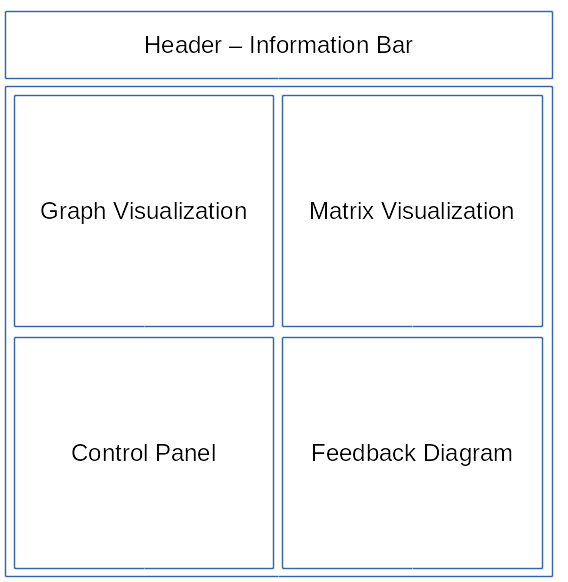
\includegraphics[width=0.44\textwidth]{explain-vis.png}
\hfill
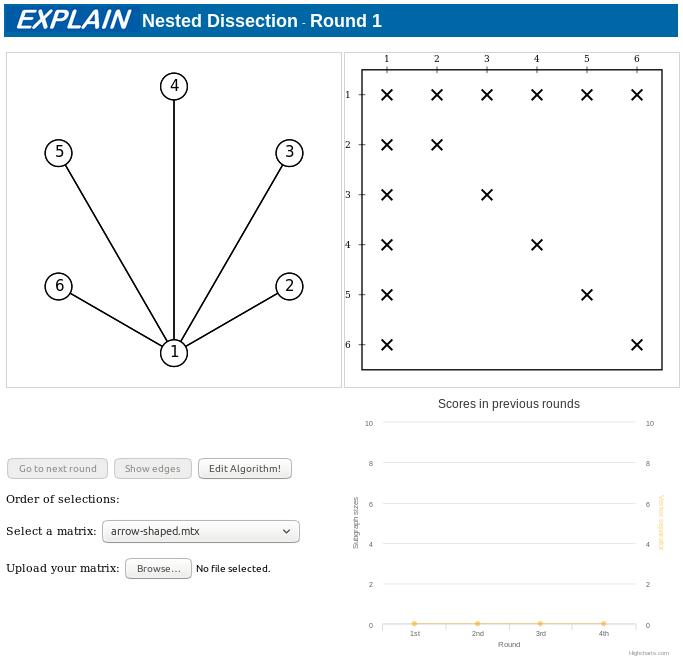
\includegraphics[width=0.48\textwidth]{explain2-init.png}
\caption{
(Left)~\mbox{EXPLAIN} has a fixed layout consists of four sections and a header.
(Right)~An example of the actual implemented view of \mbox{EXPLAIN}.}
\label{explain-design}
\end{figure}
%%%%%%%%%%%%%%%%%%%%%%%%%%%%%%%%%%%%%%%%%%%%%%%%%%%%%%%%%%%%%%%%%%%%%%%%%%%%%%%%%%%%%

We define a set of predefined colors which can be selected by
the corresponding numbers, for example
$\{1=\text{green}, 2=\text{turquoise}, 3=\text{orange}, 4=\text{violet},
5=\text{red}, 6=\text{yellow}, ...\}$.
These colors are selected such that they look perceptually distinct.
However, a user can define any new color by a function that specifies an \textbf{rgb} value.
Another aspect of the design is to use the same colors in the graph and matrix views
as well as in the feedback diagram.
This consistent use of colors in the graph
view, the matrix view, and in the feedback diagram makes it easier for the student to understand
the algorithm. We will see examples of this aspect in the different modules
which we explain in \secref{s.av.modules}.


%%%%%%%%%%%%%%%%%%%%%%%%%%%%%%%%%%%%%%%%%%%%%%%%%%%%%%%%%%%%%%%%%%%%%%%%%%%%%%%%%%%%%
\section{Gamification}
\label{s.game}
%%%%%%%%%%%%%%%%%%%%%%%%%%%%%%%%%%%%%%%%%%%%%%%%%%%%%%%%%%%%%%%%%%%%%%%%%%%%%%%%%%%%%
To engage the students more in the teaching process, we improved EXPLAIN such that the students get
more feedback from the software.
This concept is called gamification~\cite{deterding2011:gug,deterding2011}.
The use of elements from game design in the context of
computer science education is not new. In particular, programming assignments can involve
implementations of games. In \cite{la2007:gfa}, for instance, an introductory programming course is
taught under the common umbrella of two-dimensional game development. Similarly, a game project is
used in a course on software architecture~\cite{Wang2011:EEU}. Programming assignments can also
involve pieces of software that act as a player in an existing game. Rather than implementing a game, we are
interested in situations where students learn by playing a game.
A publication addressing this aspect of gamification is given in
\cite{Hakulinen2011:usg} where game-based learning is used to teach a course in data structures and
algorithms. A collaborative game is described in \cite{shl:bsc} that aims at improving the teaching
quality of a course on mathematical logic.

The gamification of \mbox{EXPLAIN} is based on finding a solution to a combinatorial scientific problem.
We interpret each solution to a problem instance as a \textit{round}.
The feedback diagram reports the results of previous rounds.
The idea of gamification is used to solve a combinatorial
minimization problem. For example, the gamification in the nested dissection ordering
consists of minimizing the size of the vertex separator while, at the same
time, balancing the sizes of the remaining components.


\section{Available modules}
\label{s.av.modules}
%%%%%%%%%%%%%%%%%%%%%%%%%%%%%%%%%%%%%%%%%%%%%%%%%%%%%%%%%%%%%%%%%%%%%%%%%%%%%%%%%%%%%
In \mbox{EXPLAIN}, we have already implemented several modules.
After discussing the module for the full unidirectional Jacobian compression using the column-intersection graph model,
we explain the modules for the full and partial bidirectional Jacobian computation.
Then, two other modules of nested dissection ordering and parallel matrix-vector
are presented to see other features of the software.
%%%%%%%%%%%%%%%%%%%%%%%%%%%%%%%%%%%%%%%%%%%%%%%%%%%%%%%%%%%%%%%%%%%%%%%%%%%%%%%%%%%%%
\subsection{Column compression}
\label{s.column-compression}
%%%%%%%%%%%%%%%%%%%%%%%%%%%%%%%%%%%%%%%%%%%%%%%%%%%%%%%%%%%%%%%%%%%%%%%%%%%%%%%%%%%%%
In \cite{2013:05,2014:01}, we presented a module of \mbox{EXPLAIN} which visualizes the
coloring algorithm for the column compression interactively.
\figurename~\ref{fig1} shows a screenshot of the column compression module.
The matrix and the corresponding column intersection graph are visualized beside each other.
In the bottom of the page, different preloaded matrices can be selected
or a new matrix can be uploaded from a file on the file system of the student's computer.
The tool provides an interactive interface for the student who can control the algorithm
such as returning to previous steps or loading different graphs and matrices.
Selecting the vertices in different orderings generates different colorings corresponding to different column compressions.

\begin{figure}
\centering
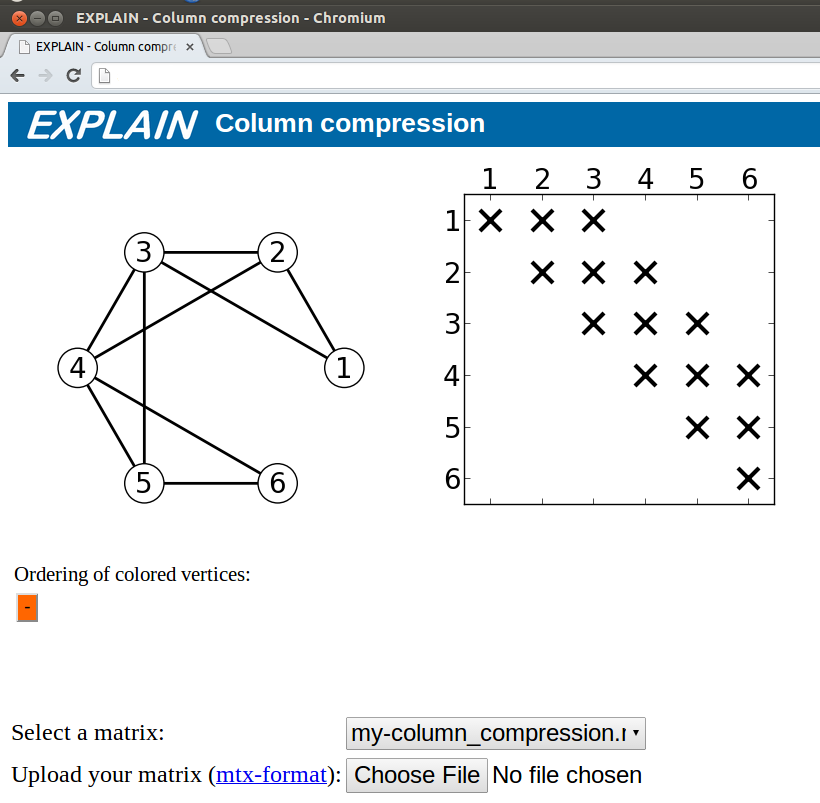
\includegraphics[width=0.5\textwidth]{fig1.png}
\caption{The initial layout of EXPLAIN for some given column compression problem.}
\label{fig1}
\end{figure}
The module allows to select and, thus, color the vertices of a given graph step by step. The order in which the vertices are colored is interactively selected by the student. In each step, when the student selects a vertex, the program checks all of its neighbors regarding the colors. A color of the current step is then greedily selected from the predefined list of colors such that it differs from the colors of those neighbors that are already colored.
%Recall that a group of columns corresponds to a set of vertices in the graph with the same color.
To indicate this, we do not color only the vertices in the graph but also the corresponding columns in the matrix.

Suppose a vertex is selected in the first step.
This vertex is then colored using the first color of the predefined list.
Continuing the process of vertex selection,
different colors are chosen and an ordered list of vertices is created
which is indicated in the subfigures of \figref{algorihtm} marked by ''Ordering of colored vertices.''
Each button of this list is clickable, causing \mbox{EXPLAIN} to return to that step of the algorithm.
The process continues until all vertices are colored.
The button labeled by the minus sign will go back to the first step.


\begin{figure}
\centering
\subfigure[Student selected $v_2$ and $v_6$ in that order.]{
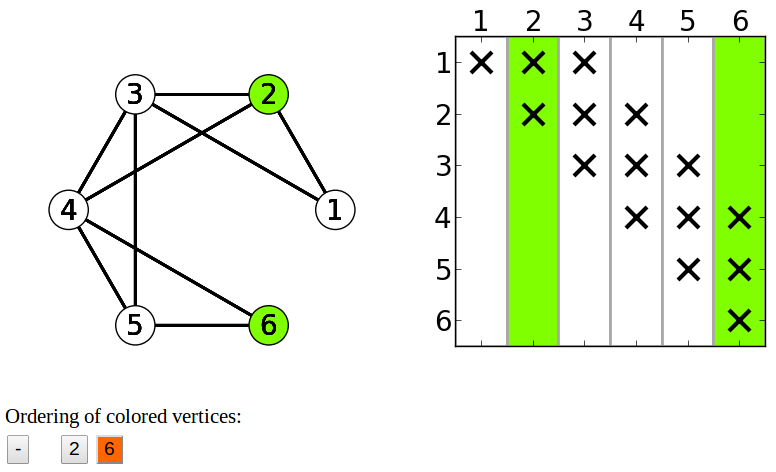
\includegraphics[width=0.47\textwidth]{fig2.png}
\label{fig2}
}
\centering
\subfigure[Student selected $v_2$, $v_6$, $v_3$, $v_5$, $v_1$, and $v_4$ in that order.]{
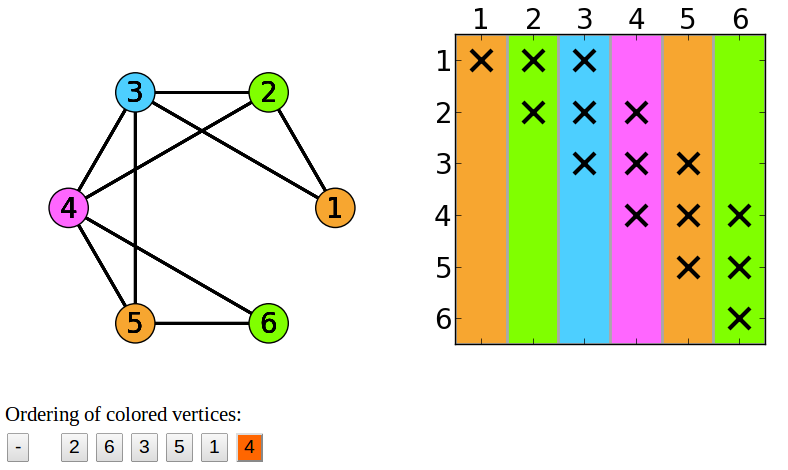
\includegraphics[width=0.47\textwidth]{fig3.png}
\label{fig3}
}
\centering
\subfigure[Student selected vertices as in \figurename~\protect\ref{fig3} and then jumped back to $v_2$.]{
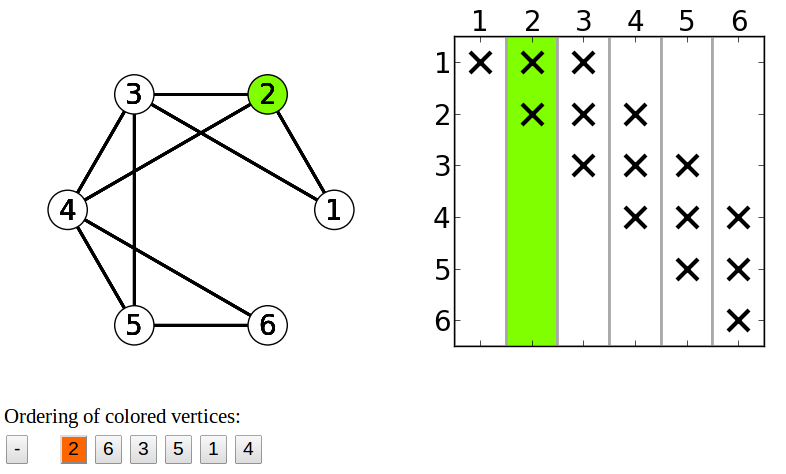
\includegraphics[width=0.47\textwidth]{fig4.png}
\label{fig4}
}
\centering
\subfigure[Student selected $v_2$, $v_1$, $v_3$, $v_4$, $v_5$, and $v_6$ in that order.]{
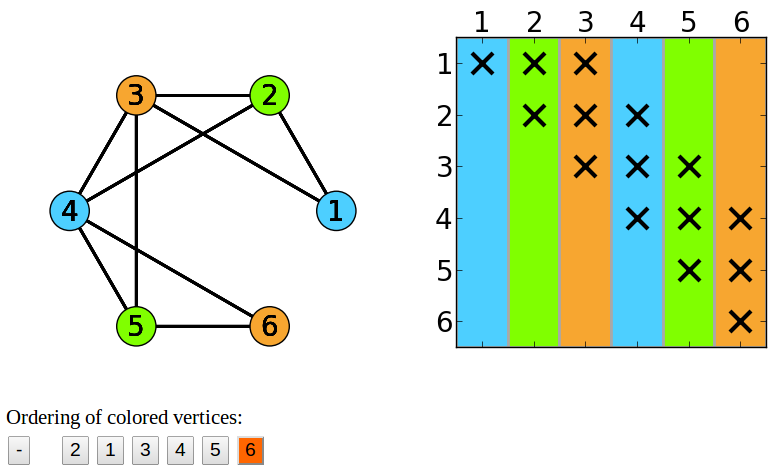
\includegraphics[width=0.47\textwidth]{fig5.png}
\label{fig5}
}
\caption{Display of various situations after interactively choosing vertices.}
\label{algorihtm}
\end{figure}
\figref{fig2} shows a representation of a nonzero pattern of the possible following matrix
\begin{equation}
\label{e:matrixJ}
J =
\begin{bmatrix}
1 & 2 & 3 & 0 & 0 & 0 \\
0 & 4 & 5 & 6 & 0 & 0 \\
0 & 0 & 7 & 8 & 9 & 0\\
0 & 0 & 0 & 10 & 11 & 12\\
0 & 0 & 0 & 0 & 13 & 14 \\
0 & 0 & 0 & 0 & 0 & 15
\end{bmatrix},
\end{equation}
and the related column-intersection graph in which the student has already selected the two vertices $v_2$ and $v_6$. Both vertices are colored with the same color since they are not connected by an edge. \figref{fig3} represents the final step which shows that four colors are needed when the vertices are selected in the order $(v_2, v_6, v_3, v_5, v_1, v_4)$ displayed in the vertex list. The group of columns with the same color is compressed to a single column in the seed matrix as follows.
\begin{equation}
\label{e:matrixS}
J \cdot S =
J \cdot
\begin{bmatrix}
 0  & 0 & 1 & 0 \\
 1  & 0 & 0 & 0 \\
 0  & 1 & 0 & 0 \\
 0  & 0 & 0 & 1 \\
 0  & 0 & 1 & 0 \\
 1  & 0 & 0 & 0
\end{bmatrix}
=
\begin{bmatrix}
2 & 3 & 1 & 0 \\
4 & 5 & 0 & 6 \\
0 & 7 & 9 & 8 \\
12 & 0 & 11 & 10\\
14 & 0 & 13 & 0 \\
15 & 0 & 0 & 0
\end{bmatrix}.
\end{equation}
Furthermore, the coloring of \figurename~\ref{fig3} is the one corresponding to that compressed Jacobian~\eqref{e:matrixS}.

Since we want to provide the possibility to return to some step of the algorithm, a history of the selection process is kept in the ordered vertex list. Now, suppose the student selects to return to the step $1$ where the vertex $v_2$ was selected, then the program returns to that step of the algorithm. The resulting state is depicted in \figref{fig4}. Notice that the program keeps the whole history and the student can click on any other buttons in the history list.

On the other hand, the student can select a completely new selection order from the current step which can generate a smaller or larger number of colors. Employing the different ordering $(v_2,v_1,v_3,v_4,v_5,v_6)$ shown in \figurename~\ref{fig5} leads to a reduction of one color compared to the first ordering given in \figurename~\ref{fig3}. In fact, this is the minimum number of colors needed to color this graph. The corresponding seed matrix is given by
$$
S =
\begin{pmatrix}
1 & 0 & 0 \\
0 & 1 & 0 \\
0 & 0 & 1 \\
1 & 0 & 0 \\
0 & 1 & 0 \\
0 & 0 & 1 \\
\end{pmatrix}.
$$
%%%%%%%%%%%%%%%%%%%%%%%%%%%%%%%%%%%%%%%%%%%%%%%%%%%%%%%%%%%%%%%%%%%%%%%%%%%%%%%%%%%%%
\subsection{Full and partial Jacobian computation}%Bidirectional compression}
\label{s.bidirectional}
%%%%%%%%%%%%%%%%%%%%%%%%%%%%%%%%%%%%%%%%%%%%%%%%%%%%%%%%%%%%%%%%%%%%%%%%%%%%%%%%%%%%%
In our publication~\cite{2014:09}, we design and implement an interactive module to
teach bidirectional compression and its connection to star bicoloring.
Figure~\ref{f.explain} shows an overview of the layout of the new module whose top and
bottom part are shown in~(a) and~(b), respectively. In the top part, a graph and a matrix
are visualized next to each other. Here, a matrix with a sparsity pattern in the form of
an arrow is taken as an example. The nonzero pattern of the matrix is shown right and the
corresponding bipartite graph is depicted left. A vertex $r_i$, which is placed on the
left part of the graph, represents the $i$th row of the matrix. Likewise, a vertex on the
right part of the graph labeled $c_i$ corresponds to the $i$th column of the matrix.

%------------------------------------------------------------------------------------------------
\begin{figure}
\centering
\subfigure[]{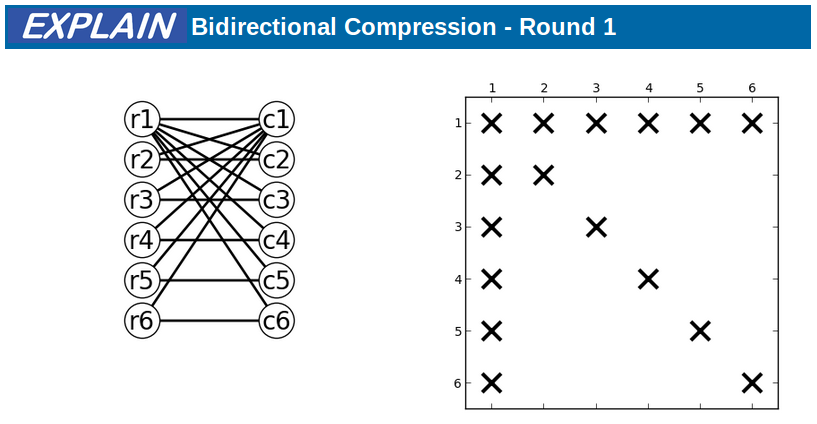
\includegraphics[width=0.43\textwidth]{init-bipartite}}
\hfill
\subfigure[]{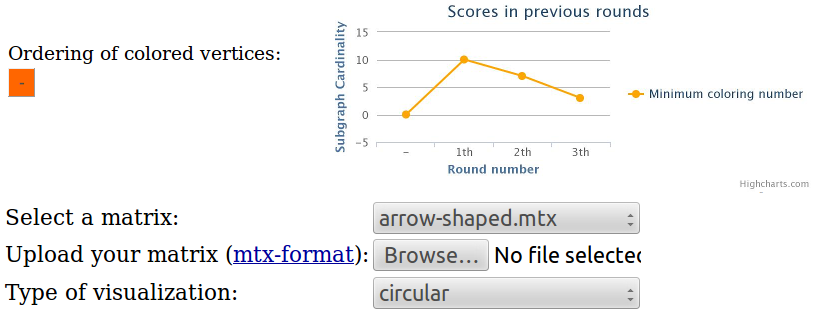
\includegraphics[width=0.55\textwidth]{explain_bottom}}
\caption{The general layout of the bidirectional compression module. (a) The top part
contains the visualization of the graph and its corresponding matrix. (b)
The bottom part contains the intermediate steps, the input, and the
history of selections.}
\label{f.explain}
\end{figure}
%------------------------------------------------------------------------------------------------


%------------------------------------------------------------------------------------------------
\begin{figure}
\centering
\subfigure[]{%
% Matrix C: after choosing 2 vertices
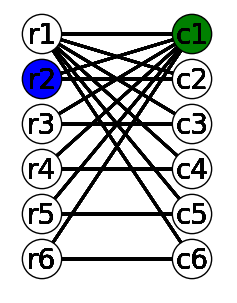
\includegraphics[width=0.18\textwidth]{arrow-shaped-bipartite-graph-twoselected}
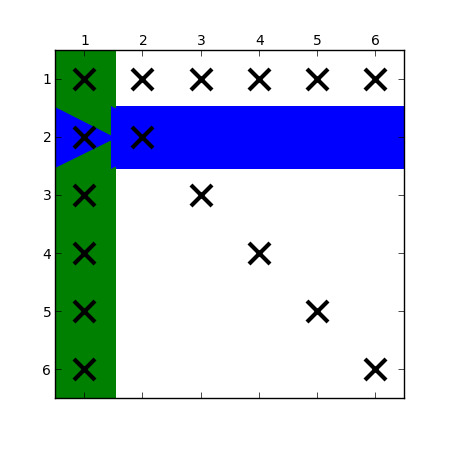
\includegraphics[width=0.26\textwidth]{arrow-shaped-matrix-twoselected}
}
\hfill
\subfigure[]{%
% Matrix C: after having completed the solution process
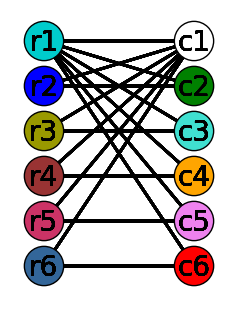
\includegraphics[width=0.18\textwidth]{arrow-shaped-almost-worst-coloring-graph}
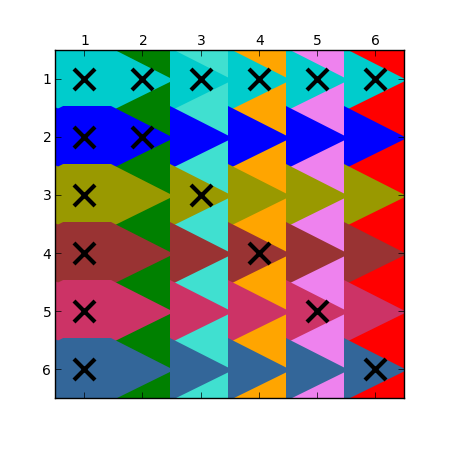
\includegraphics[width=0.26\textwidth]{arrow-shaped-almost-worst-coloring-matrix}
}%
\caption{The graph and the nonzero pattern (a) taken from Fig.~\protect\ref{f.explain}
after the student interactively selected the vertices $r_2$
and $c_1$. A star bicoloring (b) of that example after trying to solve
\MinStaBic\ interactively. This star bicoloring uses $11$ colors.}
\label{f.arrow-shaped2}
\end{figure}
%------------------------------------------------------------------------------------------------

Using any web browser, the student can interactively solve Problem~\ref{p.coloring}, \MinStaBic,
by clicking on
vertices of the bipartite graph. The selection of a vertex by a click refers to choosing
this vertex to be colored next. This coloring is visualized simultaneously in the graph
as well as in the matrix where the neutral color is the color white. By clicking on a row
vertex, the vertex itself and the corresponding row is colored. This color should obey
the rules specified in the definition of a star bicoloring. By clicking on a column
vertex, this vertex and the corresponding column are colored. Recall that a nonzero
element may be in both a colored column as well as in a colored row. In this case, we
divide the square surrounding this element into a triangle and the remaining part. The
triangle part is colored with the row color and the remaining part of the rectangle with
the column color.

%------------------------------------------------------------------------------------------------
\begin{figure}
\centering
\subfigure[]{%
% Matrix C: Minimal number of colors
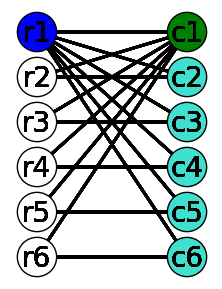
\includegraphics[width=0.18\textwidth]{arrow-shaped-best-coloring-graph}
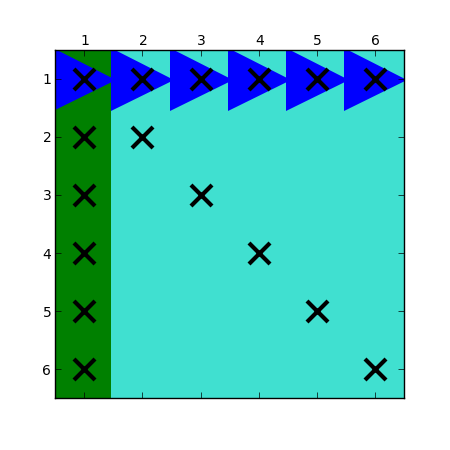
\includegraphics[width=0.26\textwidth]{arrowshaped-best-coloring-matrix}
}%
\hfill
\subfigure[]{%
% A different matrix : after having completed the solution process
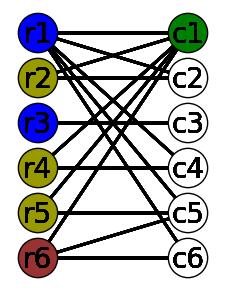
\includegraphics[width=0.18\textwidth]{arrow-shaped2-best-coloring-graph}
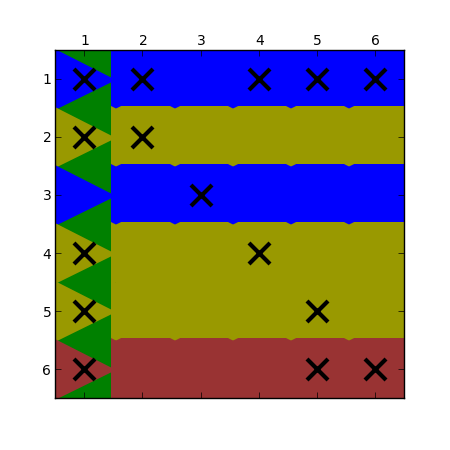
\includegraphics[width=0.26\textwidth]{arrow-shaped2-best-coloring-matrix}
}%
\caption{A star bicoloring (a) of the problem instance from
Fig.~\protect\ref{f.explain} also considered in Fig.~\protect\ref{f.arrow-shaped2}. This
star bicoloring uses $3$ colors and is an exact solution of \MinStaBic. A star bicoloring
(b) of a different problem instance using $4$ colors which is also an exact
solution of \MinStaBic} \label{f.arrow-shaped4}
\end{figure}
%------------------------------------------------------------------------------------------------

We now take the problem with the arrow-shaped nonzero pattern from Fig.~\ref{f.explain}
as an example. Here and in the following, we zoom into the graph and matrix view of the
layout. The student interactively selects a sequence of row and column vertices to solve
\MinStaBic. Figure \ref{f.arrow-shaped2} (a) shows the situation after the student
selected the vertices $r_2$ and $c_1$.
The interactive selection then goes back and forth until a correct star bicoloring is
found. Recall that the process of computing a solution of \MinStaBic\ is called a round.
The current round number is displayed at the top of the web page; see
Fig.~\ref{f.explain}~(a). When a coloring is found at round number $x$, the page shows
the message ``Round $x$ is completed!''

Selecting vertices in different orders will typically result in different star
bicolorings. A star bicoloring which is interactively chosen will not always have a
minimal number of colors. For example, the order of vertex selection visualized in
Fig.~\ref{f.arrow-shaped2}~(b) leads to a star bicoloring using $11$ colors, which is
obviously not the minimal number of colors. Here, all columns and rows are colored
differently. In contrast, Fig.~\ref{f.arrow-shaped4}~(a) illustrates an exact solution of
\MinStaBic\ for this problem instance using the minimal number of $3$ colors.

After completing a round, the student can solve the same problem instance once more. In
this case, the round number will be incremented, the colors will be removed, and another
round is started using the initial situation depicted in Fig.~\ref{f.explain}~(a). The
history of the number of non-neutral colors used in previous rounds is displayed below
the matrix in a score diagram as shown in Fig~\ref{f.explain}~(b).

The subtle issues in understanding the connection between bidirectional compression and
star bicoloring are more lucid when considering more irregularly-structured nonzero
patterns. Another problem instance with a different nonzero pattern is shown in
Fig.~\ref{f.arrow-shaped4}~(b). Here, it is more difficult to find out that this star
bicoloring with $4$ colors is indeed an exact solution to \MinStaBic.

%\subsection{Partial Jacobian computation}
We extend this module to support
the partial Jacobian computation. Here, the student should
first select the required elements which are edges in bipartite graphs.
So, when the student clicks on an edge, the color of this edge
as well as the color of the corresponding nonzero element will be changed to red.
These selected edges and nonzero elements are added to the required elements
as shown in Figure~\ref{partial_coloring_bad_coloring}.

As soon as the student starts to click the vertices, the required elements
become fixed, i.e., no new required element can be added.
The process of coloring is completely like the previous module.
Figure~\ref{partial_coloring_good_coloring} (a) shows a selection in which
the student selects only column vertices. The result is a star bicoloring
restricted to the red edges with $4$ colors.
A coloring with a smaller number of colors
is shown in Figure~\ref{partial_coloring_good_coloring} (b)
in which a row vertex is selected first.

\begin{figure}
\centering
\subfigure[]{
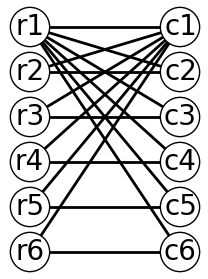
\includegraphics[width=0.18\textwidth]{arrow_shaped_partial_coloring_oneselect_graph}
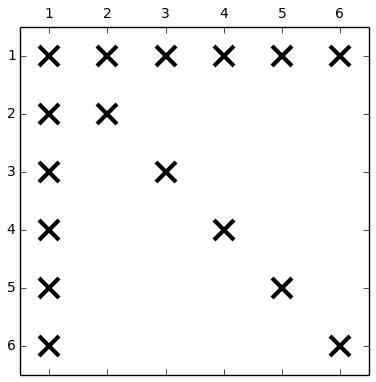
\includegraphics[width=0.26\textwidth]{arrow_shaped_partial_coloring_oneselect_matrix}}
\hfill
\subfigure[]{
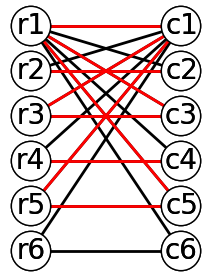
\includegraphics[width=0.18\textwidth]{arrow_shaped_partial_coloring_init_graph}
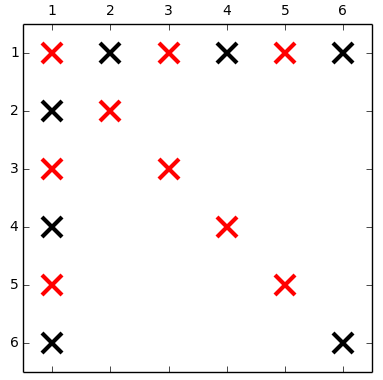
\includegraphics[width=0.26\textwidth]{arrow_shaped_partial_coloring_init_matrix}}
\caption{
(a) The initial view of the module when no required edges are selected.
(b) The user selects first the required edges. These required edges and the corresponding
nonzero elements get the red color.}
\label{partial_coloring_bad_coloring}
\end{figure}

\begin{figure}
\centering
\subfigure[]{
\includegraphics[width=0.18\textwidth]{arrow_shaped_partial_coloring_init_graph_bad_coloring}
\includegraphics[width=0.26\textwidth]{arrow_shaped_partial_coloring_init_matrix_bad_coloring}}
\hfill
\subfigure[]{
\includegraphics[width=0.18\textwidth]{arrow_shaped_partial_coloring_init_graph_good_coloring}
\includegraphics[width=0.26\textwidth]{arrow_shaped_partial_coloring_init_matrix_good_coloring}}
\caption{
(a) A graph coloring with four colors in which only column vertices are selected.
(b) A graph coloring with three colors in which the user colors a row vertex first.}
\label{partial_coloring_good_coloring}
\end{figure}

\subsection{Nested dissection ordering}
In our paper~\cite{2014:02}, we present the nested dissection module to
illustrate the connection between the following scientific computing and combinatorial problems,
\begin{problem}[Nested Dissection Ordering]
\label{p.nest.dissect}
Given a sparse symmetric positive
definite matrix $A$, find a symmetric permutation $P^T A P$ of~$A$ in the form of
\begin{equation}
\label{e.A}
A^{\prime} =
\begin{bmatrix}
A_1 & 0   & B_1^T \\[0.2em]
0   & A_2 & B_2^T \\[0.2em]
B_1 & B_2 & C
\end{bmatrix} ,
\end{equation}
such that the size of the block~$C$ is minimized while the sizes of the blocks $A_1$ and $A_2$ are
balanced.

\end{problem}
\begin{problem}[Small Vertex Separator]
\label{p.small.ver.sep} Given the graph $G$ associated with a sparse
matrix $A$, find a disjoint decomposition of the vertices $V = V_1 \cup V_2 \cup S$ with a vertex
separator $S$ such that the size of the vertex separator, $|S|$, is minimized while the sizes of
the two remaining components, $|V_1|$ and $|V_2|$, are balanced.
\end{problem}

The graph model of this problem has the simple graph layout considering the matrix
as the adjacency matrix of a graph.
The algorithm from~\cite{2014:02} searches for a vertex-separator set
corresponding to the block $C$ here. A vertex separator $S$ of the given graph $G$
is a subgraph of $G$ if the removal of $S$ and its adjacent edges from $G$ results in two
disconnected components $V_1$ and $V_2$ of $G$.
Suppose we move rows and columns corresponding to the vertex separator to the end of
the matrix and bring together
the corresponding columns of $V_1$ and $V_2$ by a permutation,
then a nested dissection would is visualized in the matrix by the block form (\ref{e.A}).

In this module representing a bisection, a round consists of finding a vertex separator.
Figure~\ref{initial_10} shows the initial layout of an example
and the selection of the vertex $v_{10}$ for the set of vertex separator.
The module moves the
column corresponding to the selected vertex to the end of the matrix
and both the vertex and its corresponding column get the orange color.
Additionally, the adjacent edges of the vertex are removed for a better visualization
(compare \figref{initial_10} (a) and \figref{initial_10} (b)).

\begin{figure}
\centering
\subfigure[]{
\includegraphics[width=0.23\textwidth]{graph_initial}
\includegraphics[width=0.23\textwidth]{matrix_initial}}
\hfill
\subfigure[]{
\includegraphics[width=0.23\textwidth]{graph_10_selected}
\includegraphics[width=0.23\textwidth]{matrix_10_selected}}
\caption{
(a) Two equivalent representations in terms of a graph and a matrix.
(b) Graph and matrix view after selecting the vertex number~10.
The decomposition into two blocks is still not shown as the graph is not yet
decomposed into two disconnected components.}
\label{initial_10}
\end{figure}

Figure~\ref{selected_4_10_8_10} shows two scenarios.
We have an unbalanced result in~\figref{selected_4_10_8_10}(a)
in which the vertex $v_4$ is selected after the initial selection of $v_{10}$.
However, \figref{selected_4_10_8_10}(b) results in a balanced result
by only selecting $v_8$ instead of $v_4$.
When a vertex separator is found,
the software performs the permutation
and colors the two disconnected components of the graph
as well as the distinct blocks on the diagonal with blue and red.

\begin{figure}
\centering
\subfigure[]{
\label{selected410}
\includegraphics[width=0.23\textwidth]{graph_4_10_selected}
\includegraphics[width=0.23\textwidth]{matrix_4_10_selected}}
\hfill
\subfigure[]{
\label{selected810}
\includegraphics[width=0.23\textwidth]{graph_8_10_selected}
\includegraphics[width=0.23\textwidth]{matrix_8_10_selected}}
\caption{
(a) Graph and matrix view after selecting the vertices number 10 and then 4.
The selection is not adequate as the sizes of blocks are not balanced.
(b) Graph and matrix view after selecting the vertices number 10 and then 8. The block sizes are balanced and the separator size is minimized.}
\label{selected_4_10_8_10}
\end{figure}

The feedback diagram from different rounds looks
like \figref{diagram}. Here, the blue and red curves should have
values close to each other since this indicates the balancing condition.
The orange curve should be as small as possible
because it represents the minimization of the separator size.
In in the last round of this figure, we see a balanced result with minimal separator size.
\begin{figure}
\centering
\includegraphics[width=0.47\textwidth]{diagram}
\caption{Score diagram resulting from four different rounds.}
\label{diagram}
\end{figure}

Based on the new features of \mbox{EXPLAIN 2.0}, we update the previous
bisection to a recursive bisection algorithm.
It contains the bisection itself. So, the student selects the vertex separator
as before until the graph becomes disconnected.
In this new version, the vertex separator is shown in orange on the bottom
of the graph. Also the two remaining components of the graph are shown separately
in two different colored circles at the top of this figure.
In Figure~\ref{bad_bisection}, the result of a selection is visualized which
is not balanced.
Figure~\ref{good_bisection} also shows the results of a more balanced selection.

\begin{figure}
\centering
\includegraphics[width=0.8\textwidth]{bad_bisection}
\caption{A selection results in an unbalanced bisection of graph.}
\label{bad_bisection}
\end{figure}

\begin{figure}
\centering
\includegraphics[width=0.8\textwidth]{good_bisection}
\caption{A selection results in a more balanced bisection of graph.}
\label{good_bisection}
\end{figure}

\begin{figure}
\centering
\includegraphics[width=0.8\textwidth]{bad_disection}
\caption{A complete nested dissection with an unbalanced result.}
\label{bad_disection}
\end{figure}


\begin{figure}
\centering
\includegraphics[width=0.8\textwidth]{good_disection}
\caption{A complete nested dissection with a better balanced result.}
\label{good_disection}
\end{figure}

\begin{figure}
\centering
\includegraphics[width=0.8\textwidth]{good_disection2}
\caption{A complete nested dissection with an even more balanced result.}
\label{good_disection2}
\end{figure}

Now, in contrast to the previous version, the student can click further
on the vertices of each component. This selection would trigger a recursive
bisection of the two components of the matrix as well. Again, this selection goes forward until
both graph components become disconnected. The vertex separators
are moved to the bottom of the graph components as well as the graph components
are shown separately.
Figure~\ref{bad_disection} and Figure~\ref{good_disection}
illustrate two unbalanced and better balanced results of nested dissection,
respectively. Figure~\ref{good_disection2} shows how the results can
get even more balanced.

The corresponding feedback diagram is modified such that
both the size of the vertex separator as well as the size of the four graph components
can be visualized. In this diagram, the separator size shows the sum of all
the vertex separators of all recursion levels.
Figure~\ref{barchart} shows a possible selection history.
The line chart shows the size history of the vertex separator
and four-bar chart grouped together shows the size history of the graph parts.
The colors are also the same colors used in the graph and matrix visualizations.
The goal here is to minimize the size of the vertex separator as well as balancing the
size of the subgraphs. We achieved a balanced results in the fourth round of selection.
\begin{figure}
\centering
\includegraphics[width=0.6\textwidth]{chart2}
\caption{The size of four subgraphs, shown as bar charts,
resulted from nested dissection compared in different rounds.
The colors of the bars are related to the colors of the corresponding subgraphs.
The curve in orange color shows the size of the vertex separator.}
\label{barchart}
\end{figure}

%%%%%%%%%%%%%%%%%%%%%%%%%%%%%%%%%%%%%%%%%%%%%%%%%%%%%%%%%%%%%%%%%%%%%%%%%%%%%%%%%%%%%%%%%%%%%%%%
\clearpage
\subsection{Parallel matrix-vector product}
%%%%%%%%%%%%%%%%%%%%%%%%%%%%%%%%%%%%%%%%%%%%%%%%%%%%%%%%%%%%%%%%%%%%%%%%%%%%%%%%%%%%%%%%%%%%%%%%
In our paper~\cite{2015:3}, we present a module for a parallel matrix-vector
product to illustrate the connection between the following scientific computing and combinatorial problems.
\begin{problem}[Data Distribution]
\label{p.par.mat.vec}
Given a large sparse matrix $A$ with a symmetric nonzero pattern and a dense
vector $x$. Suppose we want to compute the sparse matrix-vector product
$y \leftarrow Ax$ on a computer with distributed memory. Find a non-redundant
data distribution of the nonzero elements of $A$ in a row-wise fashion and a
consistent distribution of $x$ and $y$ such that the communication between
processes is minimized while the number of arithmetic operations is balanced
between the processes.
\end{problem}
\begin{problem}[Graph Partitioning]
\label{p.par.mat.vec.graph}
Given an undirected connected graph $G$, find a partition of the vertices $V$ into
nonempty disjoint subsets such that the number of edges with incident vertices
in different partitions is minimized while the number of vertices of the subsets
is balanced.
\end{problem}
These two problems are connected by letting a row $i$ of $A$ be represented by a vertex $v_i$
in $G$ and the nonzero elements in the positions $(i,j)$ and $(j,i)$ correspond to
an edge between vertices $v_i$ and $v_j$.
Let $P: V \rightarrow \{1, 2, \dots, p\}$ be the vertex partition to $p$ processes
that decomposes the set of nodes $V$ of the graph into~$p$ subsets $V_1$, $V_2$, \dots,
$V_p$ such that
$$
V = V_1 \cup V_2 \cup \dots \cup V_p
$$
with $V_i \cap V_j = \emptyset$ for~$i \neq j$. This decomposition of $V$ represents
the distribution of the rows of $A$ to $p$ processes.

Assuming that the number of nonzeros is roughly the same for each row of $A$, the
computation is evenly balanced among the $p$ processes if the partition $P$ is
$\varepsilon$-balanced defined as
\begin{equation}\label{e.bal}
\max_{1 \leq i \leq p} |V_i| \leq (1 + \varepsilon) \frac{|V|}{p} ,
\end{equation}
for some given $\varepsilon > 0$. The graph partitioning problem consists of minimizing
the number of edges with incident vertices in different partitions (the cut size)
of an $\varepsilon$-balanced partition. It is a hard combinatorial problem~\cite{gj:com}.


The parameter $\varepsilon$ introduced in~\eqref{e.bal} is used to quantify the degree of
imbalance allowed in a data distribution. If $\varepsilon = 0$ all processes are assigned
exactly $|V|/p$ rows of $A$, meaning that no imbalance is allowed at all. When
increasing $\varepsilon$ the load balancing condition~\eqref{e.bal} is relaxed. The
larger $\varepsilon$ is chosen, the larger is the allowed imbalance. Thus, in some way,
$\varepsilon$ quantifies the deviation from a perfect load balance. An equivalent form
of~\eqref{e.bal} is given by
\begin{equation}\label{e.bound}
\frac{p}{|V|} \max_{1 \leq i \leq p} |V_i| - 1 \leq \varepsilon ,
\end{equation}
which can be interpreted as follows. Suppose that you are not looking for an
$\varepsilon$-balanced partition $P$ for a given $\varepsilon$, but rather turn this
procedure around and ask: ``Given a partition $P$, how large need $\varepsilon$ at least
be so that this partition is $\varepsilon$-balanced?'' Then the left-hand side of the
inequality~\eqref{e.bound} which we call \emph{deviation bound} gives an answer to that
question. The extreme cases for the deviation bound are given by $0$ if the distribution is
perfectly balanced and $p-1$ if there is one process that gets all the data.

Figure~\ref{f.explain.matvec} shows the overall layout of this interactive
module for sparse matrix-vector multiplication.
The top of this figure visualizes
the representation of the problem regarding the graph~$G$ as well as in terms
of the matrix $A$ and the vector $x$. Below on the left, there is a panel of
colors representing different processes and another panel displaying the order of
selecting vertices of the graph. Next, on the right, there is a feedback diagram recording
values characterizing communication and load balancing.

%------------------------------------------------------------------------------------------
% Overall Layout of Module
\begin{figure}
\centering
\includegraphics[width=0.7\textwidth]{final}
\caption{Overall structure of the sparse matrix-vector multiplication module.}
\label{f.explain.matvec}
\end{figure}
%------------------------------------------------------------------------------------------

This figure gives an overall impression of the status of the module after a data
distribution is completed. Here, $p=4$ processes represented by the colors blue, green,
red, and yellow get data by interactive actions taken by the student.
Figure~\ref{f.beginning} now shows the status of the module in a phase that is more
related to the beginning of that interactive procedure. For a given matrix, the student
can distribute the data to the processes by first clicking on a color and then clicking
on an arbitrary number of vertices. That is, the distribution of vertices to a single
process is determined by first clicking on a color $j$ and then clicking on a particular
number of vertices such that these vertices are distributed to the process $j$.
Then, by clicking on the next color, this procedure can be repeated until
all vertices are interactively colored and, thus, the data distribution $P$ is finally
determined.

Figure~\ref{f.beginning} illustrates the situation after the student distributed
vertices~$\{ v_1, v_2, v_3 \}$ to the blue process
and the vertices~$\{ v_7, v_8, v_{10}\}$ to the green
process. By interactively assigning a vertex to a process, not only the vertex is colored
by the color representing this process, but also the row in the matrix as well as the
corresponding vector entry of $x$ are simultaneously colored with the same color.
This way, the data distribution is visualized in the graph and the matrix
simultaneously which emphasizes the connection between the matrix representation and the
graph representation of that problem. By inspection of the panel representing the order of selection
in~\figref{f.explain.matvec}, we find out that the status depicted in \figref{f.beginning} is an
intermediate step of the interactive session that led to the data distribution
in~\figref{f.explain.matvec}. Any box labeled with the number of the chosen vertex in that panel
is also clickable allowing the student to return to any intermediate state and start a
rearrangement of the data distribution from that state.

%------------------------------------------------------------------------------------------
% Interactive Selection of Vertices
\begin{figure}
\centering
\includegraphics[width=0.7\textwidth]{twoColors}
\caption{The intermediate state after the student selected six vertices.}
\label{f.beginning}
\end{figure}
%------------------------------------------------------------------------------------------

In this module, the problem consists of distributing all data needed to
compute the matrix-vector product to the processes. Equivalently, the distribution of all
vertices of the corresponding graph to the processes is a round. Suppose that round~2 is
completed as given in \figref{f.explain.matvec}. Then, the student can explore the data distribution in
more detail by clicking on a color in the panel labeled ``Color of processes.'' Suppose
that the student chooses the red process, then this action will modify the appearance of
the vector $x$ in the matrix representation to the state given
in~\figref{f.communication}. Here, all vector entries that need to be communicated to the
red process are now also colored red.
The background color in the vector still represents the process
that stores that vector entry.

%------------------------------------------------------------------------------------------
% Communication structure
\begin{figure}
\centering
\includegraphics[width=0.7\textwidth]{redComm}
\caption{All vector entries $x_i$ to be communicated to the red process are drawn in red.}
\label{f.communication}
\end{figure}
%------------------------------------------------------------------------------------------

After completion of a round, it is also instructive to focus on the quality of the data
distribution $P$. Recall that the graph partitioning problem aims at minimizing the cut
size of~$P$ while balancing the computational load evenly among the processes.
\figref{f.score} shows the feedback diagram. For each round, this diagram shows the cut size
using the label ``communication volume.''
In that feedback diagram, the student can attempt to minimize the communication volume over some rounds.

%------------------------------------------------------------------------------------------
% Score diagram
\begin{figure}
\centering
\includegraphics[width=0.8\textwidth]{chart}
\caption{The communication volume and the deviation bound versus various rounds.}
\label{f.score}
\end{figure}
%------------------------------------------------------------------------------------------
The feedback diagram also shows the value of the deviation bound for each round.
A low deviation bound
indicates a partition that balances the computational load evenly, whereas a large
deviation bound represents a significant imbalance of the load. The score diagram helps the
student to evaluate the quality of a single data distribution and to compare it with
distributions obtained in previous rounds. This feedback to the student is in
the spirit of computer games, where a score has only a low immediate relevance to the
current game. However, the idea is to achieve a ``high score'' and try to motivate the
player to beat that score in subsequent rounds, thus offering an extra challenge. For
this educational module, a ``high score'' would consist of a low communication value
together with a small deviation bound.

%%%%%%%%%%%%%%%%%%%%%%%%%%%%%%%%%%%%%%%%%%%%%%%%%%%%%%%%%%%%%%%%%%%%%%%%%%%%%%%%%%%%%%
\section{New features in EXPLAIN 2.0}
\label{s.alg.edit}
%%%%%%%%%%%%%%%%%%%%%%%%%%%%%%%%%%%%%%%%%%%%%%%%%%%%%%%%%%%%%%%%%%%%%%%%%%%%%%%%%%%%%%
EXPLAIN 2.0 has various features which are
discussed in the following paragraphs.
The new major feature is an algorithm editor.
In EXPLAIN 2.0, the student can see and edit the source code of an algorithm
beside the visualization of the graph and matrix.
There is a new button in the control button named as \textit{Edit Algorithm!}.
Clicking this button shows an editor with the source code of the corresponding module.
This source code is written in a simple scripting language.
Figure~\ref{f.custom_module} illustrates the column compression module.
As it can be seen, an editor with the corresponding source code of
the column compression module is shown in the right part of the figure.
Additionally, the student can see an animation of this algorithm
by first selecting and ordering and then clicking the button
named as \textit{animate}.
An animation goes through the vertices and executes each line of the algorithm
one by one to visualize the algorithm when it is executed.
The student can stop the algorithm and select the speed of execution.

Figure~\ref{f.bottom_new_explain} shows the control panel of EXPLAIN 2.0 for the
nested dissection module in the left figure and the column compression
module in the right figure.
Compared to EXPLAIN 1.0, we here have three new buttons for the three functionalities:
going to next round, doing a postprocessing, and editing an algorithm.
The first button named as \textit{Go to next round} goes to the next round even if
the current round is not completed. The second button is for a postprocessing
step. A postprocessing is an action which can be done when a round is completed.
It can be different for each module.
For example, Figure~\ref{f.bottom_new_explain} (Left) has the postprocessing named
as \textit{Show edges}. This shows the edges between the vertex separators
and the subgraphs which we remove during the selection.
Another example is Figure~\ref{f.bottom_new_explain} (Right) which does not have
any postprocessing. So, the button is disabled.
The third button is to show and hide the algorithm editor.
The label of the button is first \textit{Edit Algorithm!}
and changed to \textit{Finish Editing!} after clicking.

Another minor change is the reference to a publication which explains the
module. Figure~\ref{f.bottom_new_explain} (Left) and (Right) shows the two publications
\cite{2013:05} and \cite{2014:02} for the nested dissection and the column compression module
and the link to the publishers.
%------------------------------------------------------------------------------------------
% Custom Module
\begin{figure}
\centering
\includegraphics[width=\textwidth]{custom_module}
\caption{The code of the corresponding module is visualized beside
graph and matrix. This code is in a simple scripting language.
The user specifies the order and this code is executed based on that order.}
\label{f.custom_module}
\end{figure}
%------------------------------------------------------------------------------------------

%------------------------------------------------------------------------------------------
% Custom Module
\begin{figure}
\centering
\includegraphics[width=0.45\textwidth]{bottom_new_explain1}
\hfill
\includegraphics[width=0.45\textwidth]{bottom_new_explain}
\caption{The control panel of EXPLAIN 2.0 is visualized.
It has three new buttons for going to the next round,
doing a postprocessing step, and editing the algorithm.
Additionally, it has a new reference link to a publication
for this module.
(Left) The control panel is visualized for the nested dissection module.
Here, the postprocessing step is to show the missing edges which we remove
during the selection processes.
(Right) The control panel is visualized for the column compression module.
In this module, we do not have any postprocessing step. Hence, the button is disabled.}
\label{f.bottom_new_explain}
\end{figure}
%------------------------------------------------------------------------------------------
\section{Implementation details of EXPLAIN}
\label{s.impl.explain}
Lülfesmann et al.~\cite{Lulfesmann2010} first introduced an standalone version of EXPLAIN that
needed a client with administrator privileges to install Python libraries as well as the software itself.
Here, we introduce two new releases of EXPLAIN.
\subsection{Version 1.0}
\label{s.impl.explain1}
This section is a summary of the implementation details
of EXPLAIN 1.0 in our publication~\cite{2013:05}.
In EXPLAIN 1.0, the software is moved to the online platform which means the student needs just a web browser to work with the software.
EXPLAIN 1.0 combines several Python packages. More precisely, the graph data structure is handled by \textit{NetworkX} \cite{networkx2008}. It provides different operations like creation and deletion of vertices and edges. It also allows the programmer to access characteristic graph information such as the neighbor vertices and the number of vertices. Using this library together with \textit{matplotlib} \cite{matplotlib2007} covers the different aspects of visualization. This library produces different layouts of graphs as well as the properties of vertices and edges. The matrix manipulation and visualization are handled by \textit{Scipy}~\cite{scipy2001}, specifically the construction and the visual layout of sparse matrices.

The conversion from the standalone to the online version needs the Python library \textit{Mod\_python}~\cite{modpython2013}. It comes from the \textit{Apache} project including the Python interpreter in the given Apache web server. Using this library helps to keep the previous program structure as much as possible.

The library \textit{Mod\_python} assists to implement folder management, user interaction, cookie handling, and the web interface. Specifically, the \textit{Mod\_python} modules like \textit{Apache}, \textit{util}, and \textit{PSession} are used to migrate the previous version of \mbox{EXPLAIN} to a web version. As already mentioned, the Python interpreter is embedded into the web server by the \textit{Mod\_python} module.

In the standalone version, an event was handled by a local Python function but, in the new version, there are two sides: server and client. The web browser at the client side shows HTML websites with embedded Javascript source code while the server side is a Python server. Since the buttons are HTML buttons and the events are Javascript functions, a Javascript function submits a form to the server containing the execution request and parameters to the related Python function. Then, the called Python function writes the dynamically generated result as an HTML string to the Apache request. The server sends back the HTML string and the client shows the string as a web
page.

As an example,
the basic algorithm of coloring in the column compression module and
keeping the history is shown in the pseudo-codes given in \figurename~\ref{f:alg}. The first procedure represents what happens when a student clicks on a vertex. The second one shows how the history of matrix and graph images are loaded when the student clicks on one of the history buttons.

The first procedure, \textsc{VertexClicked}, takes the selected vertex $v$ as an input parameter. To color this vertex $v$, it finds the first color from the list $ColorList$ that is different from the colors of the neighbors of $v$. The coloring of the graph is then changed, shown, and saved as an image.
Also, the vertex $v$ is added to the ordered list, $Hist$, of selected vertices for the history.

The second procedure, \textsc{HistClicked}, takes the selected history $h$. This history will be used to find and plot the previously stored images of the matrix and the graph. Also, the variable $IsInHist$ specifies that the program is in the ``history mode'' which is important if the user selects a vertex different from the previous order. In this case, the program overwrites the current history and saves new images.

\begin{figure}
\centering
\begin{algorithmic}[1]
\State $ColorList \gets \{\text{green}, \text{turquoise}, \text{orange}, \text{violet}, ...\}$
\State $Hist \gets \{\}$\Comment{History of selected vertices.}
\State $WhereInHist \gets 0$\Comment{Where in history are we?}
\State $IsInHist \gets False$\Comment{Are we in history mode?}
\State
\Procedure{VertexClicked}{$v$}\Comment{User clicks vertex $v$.}
\State $ns\gets$ neighbors($v$)
\State $ColorIndex \gets 1$\Comment{Allowed color index}
\For{$i \gets 1$ \textbf{to} size$(ColorList)$}
\State $AllowedColor \gets True$
\For{$j \gets 1$ \textbf{to} size$(ns)$}
\If{$ColorList[i] =$ color$(ns[j])$}
\State $AllowedColor \gets False$
\EndIf
\EndFor
\If{$AllowedColor = True$}
\State $ColorIndex \gets i$
\State Break
\EndIf
\EndFor
\State Color $v$ with the color $ColorList[ColorIndex]$
\State
\If{graph and matrix images are not already saved}
\State SaveMatrix()\Comment{Using a specific name}
\State SaveGraph()\Comment{Using a specific name}
\EndIf
\If{$IsInHist = True$}
\For{$i\gets WhereInHist+1$ \textbf{to} size($Hist$)}
\State $Hist.removeElementAtPosition(i)$
\EndFor
\State $Hist$.add($v$)
\State $IsInHist \gets False$
\Else
\State $Hist$.add($v$)
\EndIf
\State Update($Hist$)\Comment Update history buttons
\EndProcedure
\State
\State
\Procedure{HistClicked}{$h$}\Comment{User clicks history $h$.}
\State OpenMatrix($h$)\Comment{Plot/load matrix with specific name}
\State OpenGraph($h$)\Comment{Plot/load graph with specific name}
\State $WhereInHist \gets find(Hist,h)$\Comment{The location of $h$}
\State $IsInHist \gets True$
\EndProcedure
\end{algorithmic}
\caption{Pseudocode of the event handling in EXPLAIN}
\label{f:alg}
\end{figure}


\subsection{Version 2.0}
\label{s.impl.explain2}
In EXPLAIN 2.0, we changed the code such that it becomes more efficient and easier to extend.
In the previous version, the module was mainly based on the Python libraries:
\textit{NetworkX} \cite{networkx2008} for the graph data structure,
\textit{matplotlib} \cite{matplotlib2007} for the visualization aspects,
\textit{Scipy}~\cite{scipy2001} for the sparse matrix computation, and
\textit{Mod\_python}~\cite{modpython2013} for the web-based version.

There were two problems with the previous implementation. First, the final visualization
of graph and matrix was always an image.
So, the time for saving and loading the image was always a problem.
Second, since the final result was HTML/JS code and the computation part was in Python,
an overhead of the server management for \textit{Mod\_python} is always added to the system.

In the new implementation, we replace all Python parts with the Javascript code.
We choose the Javascript library D3 (Data-Driven Documents)
because of its power of control and visualization.
Figure~\ref{f.graph-ds} shows an illustration
of the data structure of adjacency list for graph which is implemented in Javascript.
There is an the array representing the vertices.
Each cell of array this points to another array \textit{edges} which contains
the identity of the vertices which are neighbors of that vertex.
Here, we show that the data structure contains other properties like colors.
Using the object structure of Javascript,
it can be extended dynamically to include any other properties which may be necessary later. For example, two properties \textit{distance} and \textit{parent} are added
in the implementation of Breadth-First Search (BFS).

%-----------------------------------------------------------------------------------------------
\begin{figure}
\centering
\includegraphics[width=0.38\textwidth]{graph}
\caption{The graph data structure which is implemented in EXPLAIN 2.0.}
\label{f.graph-ds}
\end{figure}
%-----------------------------------------------------------------------------------------------
We consider a model-view-control (MVC) design pattern~\cite{osmani2012learning} for our implementation.
An important aspect of our design is the suitable connection of the
model and view. A practical approach enables the direct change in view while it keeps the
separation of the view and model.
So, we have unique ids for
edges and vertices. The unique ids for vertices are the concatenation of the
string “ver” and the actual id of the vertex. Similarly, the unique ids for edges are
defined as the concatenation of the four strings “edge”, the source vertex, “-“,
and the target vertex. The same idea applies to the matrix view. Each cell of the matrix
is accessible through a unique id combining the strings “cell”, the row index,
"-", and the column index.
Each nonzero of the matrix also gets the unique id that is built in a similar way
as the cell id, but replacing the string "cell" by the string "nnz".

The previous discussion of the view access enables us to select the
specific element and change its behavior and properties. For example, the following
code changes the color of the vertex with the id~\textit{i} to the red color
and the color of a matrix cell to the blue color,
\begin{lstlisting}
d3.select("#ver"+i).set_color(red);
d3.select("#cell"+i+"-"+j).set_color(blue);
\end{lstlisting}

Another aspect of the implementation is the order of drawing edges and
vertices. Since we do not want to draw the edges on the top of the vertices,
the edges should be drawn first. On the other hand, we draw an edge
only by getting the positions of its vertices. This direct connection helps to avoid
the several updates of view for drawing vertices and edges.
To solve this problem,
we draw the edges and vertices in order by using the grouping concepts of D3.

After the first design of the software, we then considered the actual interface
for the developer. Since we do not need all the functionality which the
programming language provides, we design a new scripting language which
has particular functions for working with matrix and graph.
Table~\ref{command-table} shows some of these functions.
\begin{table}
\begin{tabular}{ | c | c |}
\hline
neighbors($l_v$) & returns the neighbors of the list $l_v$ of vertices \\ \hline
color\_vertex($v$,$c$) & colors the vertex $v$ with the color $c$ \\\hline
color\_column($i$,$c$) & colors the column $i$ with the color $c$ \\\hline
color\_row($j$,$c$) & colors the row $j$ with the color $c$ \\\hline
min($l$) and max($l$) & finds minimum and maximum of the list of integers $l$ \\\hline
diff($A$,$B$) & finds $A - B$ \\\hline
get\_colors($l_v$) & return a list of colors of the list $l_v$ of vertices\\\hline
\end{tabular}
\caption{A list of functions available in the new scripting language.}
\label{command-table}
\end{table}

Having such scripting language empowers us to have a dynamic scripting editor
together with EXPLAIN which makes the creation of new modules efficient and fast.
The developer of a new module needs only to write the action command of the vertex
click and the global variables which he/she needs.
There are some predefined variables for required data.
As an example, the variable \textit{current} and \textit{colors}
represents the current vertex and the list of predefined colors, respectively.
The following code shows the code for the column compression
module as an example.
\begin{lstlisting}
var ns = neighbors(current);
var col_ns = get_colors(ns);
var new_col = min(diff(colors,col_ns));
color_column(current, new_col);
color_vertex(current,new_col);
\end{lstlisting}
Each module in EXPLAIN 2.0 consists of four functions with particular
name conventions. For example, the following list represents these functions
for the column compression module.
Here, all functions except the one which computes one step of the algorithm
have the ending made up from the first characters of the name of the module.
\begin{itemize}
\item column\_compression: The function which computes one step of the algorithm.
\item reference\_cc: This function defines two strings: a bibliography for a reference (\textit{reference\_text}) and the actual reference url (\textit{reference\_url}).
\item global\_cc: This function contains any global variable. Particularly, the user should define some required variables which we discuss in the following paragraph.
\item post\_processing\_cc: This is an action to a post processing button. As we discussed, the postprocessing shows the missing edges in the nested dissection module.
\end{itemize}

A sample source code showing the previous functions for the column compression algorithm is as follows.
\begin{lstlisting}
var reference_cc = function () {
    reference_text= "H. M. Buecker, M. A. Rostami, M. Luelfesmann : " +
        "An interactive educational module illustrating sparse matrix compression via graph coloring.";
    reference_url= "10.1109/ICL.2013.6644591";
};

var global_cc = function () {
    graph_format="cig";
    colors = range(0,22);
    chart_yaxis1_text = "Number of colors";
    chart_group5_text = 'Number of colors';
    start_matrix = "nestedDissection3.mtx";
    animation = true;
};

var column_compression = function() {
    var ns = neighbors(current);
    var col_ns = get_colors(ns);
    var new_col = min(diff(colors, col_ns));
    color_column(current, new_col);
    color_vertex(current, new_col);
    if (get_colored_vertices().length == currentg.vertices.length) {
     gather_round_data(min(diff(colors, get_colors(get_colored_vertices()))));
     round_completed();
    }
};

var post_processing_cc = function () {

};
\end{lstlisting}

\chapter{Conclusion and future work}
\label{conc}
This dissertation is to develop the new ideas in combinatorial scientific computing mixing AD and preconditioning which we explained in \secref{s.precond}.
In Chapter~\ref{package}, we introduce new coloring heuristics
to increase the number of potentially and additionally required elements
while the number of colors remains almost the same.
Additionally, in the same chapter,
we discussed a new heuristic for the coloring restricted to the diagonal elements.
%as well as the first ideas toward a new heuristic based on the exact coloring in the small subgraphs.
%We should do more evaluations and computations for these heuristics later.
We implemented all these heuristics in our software \textit{PreCol} which
is explained in \secref{s.extend}.

Inn \secref{explain}, we develop an interactive educational module
for teaching the concepts of combinatorial scientific computing.
In this chapter, we discussed our previous publications
\cite{2013:05,2014:01,2014:02,2014:09,2015:3} and also the new features which
we have not published yet. There is still room
for new ideas in this software. Beside developing new modules,
we need to improve the usability and extensibility of the software.
Also, we need an extensive evaluation of the software to find
the new ways of further developments.

Although we proposed different heuristics, many dimensions of the problem can be improved.
We considered only the ILU preconditioning. A future work is to replace ILU
with other preconditioning techniques.
For example, the approximate inverse preconditioning (AINV)~\cite{ainv98} might be a
suitable candidate which produces no fill-in.
Another future work is to consider blocks of submatrices for coloring instead of just a complete row or column? Steihaug and Hossain~\cite{Steihaug1997GCa} discuss this idea for blocks of rows and the same column intersection graph model as before and show it has advantages in the unidirectional coloring. A first improvement is to search for the similar approach in the bidirectional coloring and restricted coloring. Finally, a new area is to look at the same ideas for the hypergraph model for fine-grained coloring.

\bibliographystyle{IEEEtran}
\bibliography{refs}
\chapter*{Appendix}
\label{appendix}
\setcounter{chapter}{1}
\addcontentsline{toc}{chapter}{Appendix}
\renewcommand\thechapter{\Alph{chapter}}
%%%%%%%%%%%%%%%%%%%%%%%%%%%%%%%%%%%%%%%%%%%%%%%%%%%%%%%%%%%
\section{Comparing the computations of Algorithm 3.1 and Algorithm 3.2}
\label{app.compare.alg31.alg32}
%%%%%%%%%%%%%%%%%%%%%%%%%%%%%%%%%%%%%%%%%%%%%%%%%%%%%%%%%%%
Here, we illustrate the figures for the comparison of Algorithm 3.1 and Algorithm 3.2.
Each figure contains three computations: potentially required elements in the top figure,
additionally required elements in the middle figure, and the number of colors in the bottom figure.
\figref{ex33_alg31_alg32_bls_nat}, \figref{ex33_alg31_alg32_bls_lfo},
and \figref{ex33_alg31_alg32_bls_slo} are for the computation for the natural ordering,
the LFO ordering, and the SLO ordering, respectively.
Also, \figref{crystm01_alg31_alg32_bls_nat} shows this comparison for the matrix \textit{crystm01}
with the natural ordering.
\begin{figure}
\centering{
\includegraphics[width=0.75\linewidth]{ex33_alg31_alg32_bls_nat_pot}
\includegraphics[width=0.75\linewidth]{ex33_alg31_alg32_bls_nat_add}
\includegraphics[width=0.75\linewidth]{ex33_alg31_alg32_bls_nat_cols}
}
\caption{The computation carried out the matrix \textit{ex33} and for the natural ordering.}
\label{ex33_alg31_alg32_bls_nat}
\end{figure}

\begin{figure}
\centering
\includegraphics[width=0.75\linewidth]{ex33_alg31_alg32_bls_lfo_pot}
\includegraphics[width=0.75\linewidth]{ex33_alg31_alg32_bls_lfo_add}
\includegraphics[width=0.75\linewidth]{ex33_alg31_alg32_bls_lfo_cols}
\caption{The computation carried  out the matrix \textit{ex33} and for the LFO ordering.}
\label{ex33_alg31_alg32_bls_lfo}
\end{figure}

\begin{figure}
\centering
\includegraphics[width=0.75\linewidth]{ex33_alg31_alg32_bls_slo_pot}
\includegraphics[width=0.75\linewidth]{ex33_alg31_alg32_bls_slo_add}
\includegraphics[width=0.75\linewidth]{ex33_alg31_alg32_bls_slo_cols}
\caption{The computation carried  out the matrix \textit{ex33} and for the SLO ordering.}
\label{ex33_alg31_alg32_bls_slo}
\end{figure}

\begin{figure}
\centering
\includegraphics[width=0.75\linewidth]{crystm01_alg31_alg32_bls_nat_pot}
\includegraphics[width=0.75\linewidth]{crystm01_alg31_alg32_bls_nat_add}
\includegraphics[width=0.75\linewidth]{crystm01_alg31_alg32_bls_nat_cols}
\caption{The computation carried  out the matrix \textit{crystm01} and for the natural ordering.}
\label{crystm01_alg31_alg32_bls_nat}
\end{figure}

\clearpage
%%%%%%%%%%%%%%%%%%%%%%%%%%%%%%%%%%%%%%%%%%%%%%%%%%%%%%%%%%%
\section{Comparing the computations of Algorithm 3.2 and Algorithm 3.4}
\label{app.compare.alg32.alg34}
%%%%%%%%%%%%%%%%%%%%%%%%%%%%%%%%%%%%%%%%%%%%%%%%%%%%%%%%%%%
\begin{table}
\centering
\begin{tabular}{|c|c|c|c|c|c|c|}
\hline
Matrix (NAT) & \multicolumn{2}{c|}{$|R_a|$} & \multicolumn{2}{c|}{$|R_p|$} & \multicolumn{2}{c|}{$|\Phi|$}\\\hline
{} & Alg.\ref{code.new.d2.nreq}& Alg.\ref{code.new.impr1} & Alg.\ref{code.new.d2.nreq} & Alg.\ref{code.new.impr1}& Alg.\ref{code.new.d2.nreq} & Alg.\ref{code.new.impr1}\\\hline
\textit{steam1.mtx} & $630$ & $64$ & $786$ & $64$ & $10$ & $7$\\\hline
\textit{steam2.mtx} & $1400$ & $240$ & $1880$ & $240$ & $17$ & $9$\\\hline
\textit{nos3.mtx} & $4296$ & $1106$ & $6756$ & $1638$ & $19$ & $13$\\\hline
\textit{ex7.mtx} & $25054$ & $29174$ & $34954$ & $38554$ & $55$ & $56$\\\hline
\textit{ex33.mtx} & $5572$ & $4920$ & $8934$ & $7408$ & $18$ & $18$\\\hline
\textit{crystm01.mtx} & $28318$ & $10388$ & $47556$ & $17822$ & $22$ & $14$\\\hline
\textit{coater1.mtx} & $7448$ & $7684$ & $11558$ & $11722$ & $27$ & $28$\\\hline
\textit{pesa.mtx} & $33094$ & $31010$ & $41154$ & $36972$ & $13$ & $12$\\\hline
\end{tabular}
\vspace*{1cm}\newline
\begin{tabular}{|c|c|c|c|c|c|c|}
\hline
Matrix (LFO) & \multicolumn{2}{c|}{$|R_a|$} & \multicolumn{2}{c|}{$|R_p|$} & \multicolumn{2}{c|}{$|\Phi|$}\\\hline
{} & Alg.\ref{code.new.d2.nreq}& Alg.\ref{code.new.impr1} & Alg.\ref{code.new.d2.nreq} & Alg.\ref{code.new.impr1}& Alg.\ref{code.new.d2.nreq} & Alg.\ref{code.new.impr1}\\\hline
\textit{steam1.mtx} & $666$ & $64$ & $1048$ & $64$ & $12$ & $7$\\\hline
\textit{steam2.mtx} & $1248$ & $240$ & $2624$ & $240$ & $17$ & $9$\\\hline
\textit{nos3.mtx} & $4442$ & $1246$ & $6882$ & $1880$ & $21$ & $16$\\\hline
\textit{ex7.mtx} & $24060$ & $28904$ & $33426$ & $37080$ & $53$ & $59$\\\hline
\textit{ex33.mtx} & $6888$ & $7170$ & $10564$ & $10574$ & $18$ & $19$\\\hline
\textit{crystm01.mtx} & $21194$ & $12256$ & $36634$ & $20326$ & $17$ & $17$\\\hline
\textit{coater1.mtx} & $7536$ & $7410$ & $11512$ & $11312$ & $24$ & $24$\\\hline
\textit{pesa.mtx} & $31884$ & $31790$ & $41676$ & $42490$ & $11$ & $11$\\\hline
\end{tabular}
\vspace*{1cm}\newline
\begin{tabular}{|c|c|c|c|c|c|c|}
\hline
Matrix (SLO) & \multicolumn{2}{c|}{$|R_a|$} & \multicolumn{2}{c|}{$|R_p|$} & \multicolumn{2}{c|}{$|\Phi|$}\\\hline
{} & Alg.\ref{code.new.d2.nreq}& Alg.\ref{code.new.impr1} & Alg.\ref{code.new.d2.nreq} & Alg.\ref{code.new.impr1}& Alg.\ref{code.new.d2.nreq} & Alg.\ref{code.new.impr1}\\\hline
\textit{steam1.mtx} & $754$ & $64$ & $1294$ & $64$ & $14$ & $7$\\\hline
\textit{steam2.mtx} & $1912$ & $240$ & $3192$ & $240$ & $17$ & $9$\\\hline
\textit{nos3.mtx} & $4382$ & $1132$ & $6772$ & $1682$ & $21$ & $13$\\\hline
\textit{ex7.mtx} & $24164$ & $27044$ & $34448$ & $36486$ & $55$ & $51$\\\hline
\textit{ex33.mtx} & $7138$ & $5186$ & $10754$ & $8024$ & $20$ & $17$\\\hline
\textit{crystm01.mtx} & $26782$ & $14252$ & $45166$ & $24478$ & $20$ & $16$\\\hline
\textit{coater1.mtx} & $7878$ & $7004$ & $11702$ & $10476$ & $24$ & $21$\\\hline
\textit{pesa.mtx} & $34044$ & $29034$ & $44624$ & $39606$ & $13$ & $10$\\\hline
\end{tabular}

\caption{The comparison between the number of potentially and additionally required
elements as well as the number of colors computed with \coderef{code.new.impr1} and \ref{code.new.d2.nreq}.
The block size is fixed to $10$. The orderings for coloring are (Top) the natural ordering,
(Middle) LFO, and (Bottom) SLO.}
\label{mats.pot.add.modified.vs.nreq}
\end{table}

%%%%%%%%%%%%%%%%%%%%%%%%%%%%%%%%%%%%%%%%%%%%%%%%%%%%%%%%%%%
\clearpage
\section{Comparing the computations of Algorithm 3.5 with different block sizes}
\label{app.compare.alg35.alphas}
%%%%%%%%%%%%%%%%%%%%%%%%%%%%%%%%%%%%%%%%%%%%%%%%%%%%%%%%%%%
Here is the comparison of the number of colors and the number of additionally required elements
prodcued by Algorithm 3.5 with different values of $\alpha$ and the varying block sizes.

\begin{figure}
\centering
\includegraphics[width=0.9\linewidth]{ex33_alg35_alpha_0_2_6_10_bls_lfo_cols}
\caption{
The comparison of the number of colors in \coderef{code.new.impr2}
with $\alpha\in{0,2,6,10}$ and the LFO ordering.}
\label{ex33_alg35_alpha_0_2_6_10_bls_lfo_cols}
\end{figure}

\begin{figure}
\centering
\includegraphics[width=0.9\linewidth]{ex33_alg35_alpha_0_2_6_10_bls_lfo_adds}
\caption{
The comparison of the number of additionally required elements in \coderef{code.new.impr2}
with $\alpha\in{0,2,6,10}$ and the LFO ordering. }
\label{ex33_alg35_alpha_0_2_6_10_bls_lfo_adds}
\end{figure}

\end{document}
